% #############################################################################
% This is the MAIN DOCUMENT of the Thesis MSc TEMPLATE.
% The content for the Thesis MSc is to be written in separate documents
% located in the folder ./Chapters
%         Aknowledgments.tex
%         Abstract.tex
%         KeyWords.tex
%         Resumo.tex
%         PalavrasChave.tex
%         Acronyms.tex
%         Front_Cover.tex
%         Chapter_1.tex ....Chapter_2 .....
%         ApendixA.tex ... ApendixB.tex...
% -----------------------------------------------------------------------------
% The class "istulthesis" is based on the standard LaTeX 'report' class.
% It can be used for Instituto Superior Tecnico thesis, as it follows the 
% regulations published by the Scientific Council of IST.
% The class defines the document style. 
% IST requires the thesis to be written in Arial or similar. 
% Two arguments in '\documentclass' allow you to define the thesis font: 
% 'Helvetica' and 'AvantGarde', which transforms 
% the default LaTeX font into Helvetica or AvantGarde, respectively.
% #############################################################################
% The document is automatically set for english or portuguese by just selecting
% the MAIN LANGUAGE in file 'Thesis-MSc-Preamble_commands.tex' 
% #############################################################################
% Thesis-MSc
% Version 4, August 2022
% BY: Prof. Rui Santos Cruz, rui.s.cruz@tecnico.ulisboa.pt
% #############################################################################
% !TEX root = ./main.tex
% -----------------------------------------------------------------------------
%
%\documentclass[defaultstyle,10pt,Helvetica,oneside]{istulthesis}
\documentclass[defaultstyle,10pt,Helvetica]{istulthesis}
%
% -----------------------------------------------------------------------------
% The Preamble document contains all the necessary Packages for typesetting
% Modify it to suit your needs
% -----------------------------------------------------------------------------
% #############################################################################
% Preamble for Thesis-MSc in English or Portuguese
% Required Packages and commands
% --> Please Choose the MAIN LANGUAGE for the Thesis in package BABEL (below)
% !TEX root = ./main.tex
% #############################################################################
% Thesis-MSc
% Version 4, August 2022
% BY: Prof. Rui Santos Cruz, rui.s.cruz@tecnico.ulisboa.pt
% #############################################################################
%
% -----------------------------------------------------------------------------
% PACKAGES ucs, utf8x, babel, iflang:
% -----------------------------------------------------------------------------
% The 'ucs' package provides support for using UTF-8 in LaTeX documents. 
% However in most situations it is not required.
\usepackage{ucs}
% The 'utf8x' package contains support for using UTF-8 as input encoding. 
\usepackage[utf8x]{inputenc}
% The 'babel' package may correct some hyphenation issues of LaTeX. 
% Select your MAIN LANGUAGE for the Thesis with the 'main=' option.
\usepackage[main=english,portuguese]{babel}
% The 'iflang' package is used to help determine the language being used. 
\usepackage{iflang}

% -----------------------------------------------------------------------------
% PACKAGE scrbase:
% -----------------------------------------------------------------------------
% The 'scrbase' package is used to help redefining document structure.
\usepackage{scrbase}
% -----------------------------------------------------------------------------
% PACKAGE mathtools, amsmath, amsthm, amssymb, a\ac{MSF}onts, nicefrac:
% -----------------------------------------------------------------------------
% These packages are typically required. 
% Among many other things they add the possibility to put symbols in bold
% by using \boldsymbol (not \mathbf); defines additional fonts and symbols;
% adds the \eqref command for citing equations.
\usepackage{mathtools, amsmath, amsthm, amssymb, amsfonts, physics}
\usepackage{blkarray} % Required for blockarray environment
\usepackage{nicefrac}

\newtheorem{theorem}{Theorem}[section]
\newtheorem{remark}[theorem]{Remark}
\newtheorem{corollary}[theorem]{Corollary}
\newtheorem{proposition}[theorem]{Proposition}
\newtheorem{lemma}[theorem]{Lemma}
\newtheorem{definition}[theorem]{Definition}
\newtheorem{conjecture}[theorem]{Conjecture}
\newtheorem{example}[theorem]{Example}

\DeclareMathOperator{\Span}{span}
\DeclareMathOperator{\dom}{Dom}
\DeclareMathOperator\supp{supp}
\DeclareMathOperator\Div{div}
\DeclareMathOperator{\atantwo}{atan2}
%
% -----------------------------------------------------------------------------
% PACKAGE tikz:
% -----------------------------------------------------------------------------
% Tikz  for creating graphics programmatically.
\usepackage{tikz}
\usetikzlibrary{shapes.geometric, arrows, positioning, angles, quotes}
\usetikzlibrary{decorations.pathmorphing}
\usepackage{siunitx}
% -----------------------------------------------------------------------------
% PACKAGES array, booktabs, multirow, colortbl, spreadtab:
% -----------------------------------------------------------------------------
% These packages are most usefull for advanced tables. 
% 'multirow' allows to join rows throuhg the command \multirow which works
% similarly with the command \multicolumn.
% The 'colortbl' package allows to color the table (foreground and background)
% The package 'booktabs' provide some additional commands to enhance
% the quality of tables
% The 'longtable' package is only required when tables extend beyond the length
% of one page, which typically does not happen and should be avoided
\usepackage{array}
\usepackage{booktabs}
\usepackage{multirow}
\usepackage{colortbl}
\usepackage{spreadtab}
\usepackage{longtable}
\usepackage{pdflscape}
\usepackage{float}
\usepackage{flafter} 
%
% -----------------------------------------------------------------------------
% PACKAGES graphicx, subfigure:
% -----------------------------------------------------------------------------
% The package 'graphicx' supports formats PNG and JPG.
% Package 'subfigure' allows to place figures within figures with own caption. 
% For each of the subfigures use the command \subfigure.
\usepackage{graphicx}
\usepackage[hang,small,bf,tight]{subfigure}
% -----------------------------------------------------------------------------
% PACKAGE caption:
% -----------------------------------------------------------------------------
% The 'caption' package offers customization of captions in floating 
% environments such figure and table
% \usepackage[hang,small,bf]{caption}
\usepackage[format=hang,labelfont=bf,font=small]{caption} 
% the following customization adds vertical space between caption and the table
\captionsetup[table]{skip=10pt}
%
% -----------------------------------------------------------------------------
% PACKAGE algorithmic, algorithm, algorithm2e:
% -----------------------------------------------------------------------------
% These packages are required if you need to describe an algorithm.
% The preference is for using 'algorithm2e'
%\usepackage{algorithmic}
%\usepackage[chapter]{algorithm}
\usepackage[ruled,vlined,algochapter,norelsize,\languagename]{algorithm2e}
%
% -----------------------------------------------------------------------------
% PACKAGE listings
% -----------------------------------------------------------------------------
% These packages are required if you need to list code snippets.
\usepackage{listings}
% Nicely syntax highlighted m-code in LaTeX documents with stylefile mcode.sty
% http://www.mathworks.com/matlabcentral/fileexchange/8015-m-code-latex-package
\usepackage[numbered]{mcode}
%
% -----------------------------------------------------------------------------
% Re-define listings captions and titles based on language.
\newcaptionname{english}{\lstlistingname}{Listagem} % Listings CAPTIONS
\newcaptionname{english}{\lstlistlistingname}{Listagens} % LIST of LISTINGS
%
% -----------------------------------------------------------------------------
% PACKAGE csquotes
% -----------------------------------------------------------------------------
% Quotation helper package
% \usepackage{csquotes}
\usepackage{epigraph}
%
% -----------------------------------------------------------------------------
% PACKAGE todonotes
% -----------------------------------------------------------------------------
% Create TODO Notes in text
% The notes can be made invisible by just using the 'disable' option:
\usepackage[textwidth=2cm, textsize=small]{todonotes}
%\usepackage[textwidth=2cm, textsize=small, disable]{todonotes}
\setlength{\marginparwidth}{2cm}
%
% -----------------------------------------------------------------------------
% PACKAGE changes
% -----------------------------------------------------------------------------
% Track changes in document (changes in pdf preview).
%% Use "final" option to make all tracking markups invisible.
%\usepackage[authormarkup=superscript,authormarkuptext=id,markup=underlined,ulem={ULforem,normalbf},final]{changes}
\usepackage[authormarkup=superscript,authormarkuptext=id,markup=underlined,ulem={ULforem,normalbf}]{changes}
% commands:
% \added[id=xx]{text}
% \deleted[id=xx]{text}
% \replaced[id=xx]{deleted text}{added text}
% -----------------------------------------------------------------------------
% PACKAGES xcolor, color
% -----------------------------------------------------------------------------
% These packages are required for list code snippets.
\usepackage{xcolor}
\usepackage{color}
% The following special color definitions are used in the IST Thesis
\definecolor{forestgreen}{RGB}{34,139,34}
\definecolor{orangered}{RGB}{239,134,64}
\definecolor{lightred}{rgb}{1,0.4,0.5}
\definecolor{orange}{rgb}{1,0.45,0.13}	
\definecolor{darkblue}{rgb}{0.0,0.0,0.6}
\definecolor{lightblue}{rgb}{0.1,0.57,0.7}
\definecolor{gray}{rgb}{0.4,0.4,0.4}
\definecolor{lightgray}{rgb}{0.95, 0.95, 0.95}
\definecolor{darkgray}{rgb}{0.4, 0.4, 0.4}
\definecolor{editorGray}{rgb}{0.95, 0.95, 0.95}
\definecolor{editorOcher}{rgb}{1, 0.5, 0} % #FF7F00 -> rgb(239, 169, 0)
\definecolor{chaptergrey}{rgb}{0.6,0.6,0.6}
\definecolor{editorGreen}{rgb}{0, 0.5, 0} % #007C00 -> rgb(0, 124, 0)
\definecolor{olive}{rgb}{0.17,0.59,0.20}
\definecolor{brown}{rgb}{0.69,0.31,0.31}
\definecolor{purple}{rgb}{0.38,0.18,0.81}
%
% -----------------------------------------------------------------------------
% PACKAGE setspace:
% ----------------------------------------------------------------------------
% Provides support for setting the spacing between lines in a document. 
% Package options include single spacing, one half spacing, and double spacing. 
% Alternatively the spacing can be changed as required with:
% \singlespacing, \onehalfspacing, and \doublespacing commands
%\usepackage{setspace}
%
% -----------------------------------------------------------------------------
% PACKAGE paralist
% -----------------------------------------------------------------------------
% This package provides the 'inparaenum' environment for inline lists
\usepackage{paralist}
% usage:
% \begin{inparaenum}[(a)]
% \item bla
% \item bla, bla
% \end{inparaenum}
% -----------------------------------------------------------------------------
% PACKAGE cite:
% -----------------------------------------------------------------------------
% The 'cite' package will result in citation numbers being automatically
% sorted and properly "ranged". i.e.,
% [1], [2], [5]--[7], [9]
\usepackage{cite}
%
% -----------------------------------------------------------------------------
% PACKAGE acronym:
% -----------------------------------------------------------------------------
% The package 'acronym' garantees that all acronyms definitions are 
% given at the first usage. 
% IMPORTANT: do not use acronyms in titles/captions; otherwise the definition 
% will appear on the table of contents.
\usepackage[printonlyused]{acronym}
%
% -----------------------------------------------------------------------------
% PACKAGE hyperref
% -----------------------------------------------------------------------------
% Set links for references and citations in document
\usepackage{hyperref}
% pre-configuration of hyperref
\hypersetup{ colorlinks=true,
             citecolor=cyan,
             linkcolor=darkgray,
             urlcolor=teal,
             breaklinks=true,
             bookmarksnumbered=true,
             bookmarksopen=true,
}
%
% -----------------------------------------------------------------------------
% PACKAGE url:
% -----------------------------------------------------------------------------
% Provides better support for handling and breaking URLs.
\usepackage{url} 
%
% -----------------------------------------------------------------------------
% PACKAGE Cleveref:
% -----------------------------------------------------------------------------
% Clever Referencing of document parts
% use \Cref[], or \cref[] for referencing items (Figures, Tables, Algorythms, 
% Equations, Chapters, Sections, etc. No need to write the Name of the item. 
% Note: portuguese is supported through "brazilian" option
\usepackage[\IfLanguageName{english}{english}{brazilian}]{cleveref}
%
% -----------------------------------------------------------------------------
% PACKAGE enumitem:
% -----------------------------------------------------------------------------
%For enhanced enumeration of lists
%\usepackage{enumitem}
\usepackage[shortlabels]{enumitem}
\setlist[description]{leftmargin=\parindent,labelindent=\parindent,itemsep=1pt,parsep=0pt,topsep=0pt}
%
% -----------------------------------------------------------------------------
% PACKAGE glossaries-extra:
% -----------------------------------------------------------------------------
% Allows creating a list of terms with definitions for those terms
\usepackage[xindy,toc,nopostdot]{glossaries}
\usepackage{glossaries-extra} 

% Special style to print trailing dots before locations list
\makeatletter
\newglossarystyle{mystyle}{%
  \setglossarystyle{altlist}%
  \renewenvironment{theglossary}{%
  \begin{description}[style=standard,labelindent=0pt,itemsep=5pt]%
  }%
  {\end{description}}
  \renewcommand*{\glossentry}[2]{%
    \item[\glsentryitem{##1}%
      \glstarget{##1}{\glossentryname{##1}}]%
      \mbox{}\par\nobreak\@afterheading
      \glossentrydesc{##1}\glspostdescription
      {\def\hfill{\hskip 25pt plus 3fill}\dotfill\mbox{ ##2}}%
  }%
  \renewcommand{\glsgroupskip}{}%
}
\makeatother
\setglossarystyle{mystyle}

% \makeglossaries
% \newglossaryentry{Hahn-Banach Theorem}{
    name={Hahn-Banach Theorem},
    description={A fundamental result in functional analysis}
}
% #############################################################################
% GLOBAL FORMATTING OF THE THESIS DOCUMENT before using FANCY stuff
% Load Titlepage definition
\usepackage{./Thesis-MSc-cover-titlepage}

% Set paragraph counter to alphanumeric mode
% DO NOT CHANGE these lines, otherwise the document will not respect the Guide
\renewcommand{\theparagraph}{\Alph{paragraph}~--}
\hoffset 0in
\voffset 0in
\oddsidemargin 0 cm
\evensidemargin 0 cm
\marginparsep 0in
\topmargin -0.25cm
\textwidth 16 cm
\textheight 22.4 cm
\makeatletter
% package indentfirst says \let\@afterindentfalse\@afterindenttrue
% and we revert this modification, reinstating the original definitio
% of \@afterindentfalse
\def\@afterindentfalse{\let\if@afterindent\iffalse}
\makeatother
% -----------------------------------------------------------------------------
% PACKAGE fancyhdr:
% -----------------------------------------------------------------------------
% The fancyhdr macro package allows to customize page headers and footers.
\usepackage{fancyhdr}
\pagestyle{fancy}
\renewcommand{\chaptermark}[1]{\markboth{\thechapter.\ #1}{}}
\renewcommand{\sectionmark}[1]{\markright{\thesection\ #1}}
\fancyhf{}
%#########################################################
% Choose the positioning of the Page Number
% Only on the Center side [C]
\fancyfoot[C]{\bfseries\thepage}
% Only on the Right side [R]
%\fancyfoot[R]{\bfseries\thepage}
% In case of Double sided printing, numbers are printed on Left (even pages) and on Right (odd pages)
%\fancyfoot[LE,RO]{\bfseries\thepage}
%#########################################################
\renewcommand{\headrulewidth}{0.0pt}
\renewcommand{\footrulewidth}{0.0pt}
\addtolength{\headheight}{2pt} % make space for the rule

\fancypagestyle{plain}{%
   \renewcommand{\headrulewidth}{0pt} % and the line
   \renewcommand{\footrulewidth}{0pt}
}
\fancypagestyle{blank}{%
   \renewcommand{\headrulewidth}{0pt} % and the line
   \renewcommand{\footrulewidth}{0pt}
}
\fancypagestyle{abstract}{%
   \renewcommand{\headrulewidth}{0pt}
   \renewcommand{\footrulewidth}{0.0pt}
}
\fancypagestyle{document}{%
	\renewcommand{\headrulewidth}{0.5pt}
	\renewcommand{\footrulewidth}{0.5pt}
	\addtolength{\headheight}{2pt} % make space for the rule
}
\setcounter{secnumdepth} {5}
\setcounter{tocdepth} {5}
\renewcommand{\thesubsubsection}{\thesubsection.\Alph{subsubsection}}
\renewcommand{\subfigtopskip}{0.3 cm}
\renewcommand{\subfigbottomskip}{0.2 cm}
\renewcommand{\subfigcapskip}{0.3 cm}
\renewcommand{\subfigcapmargin}{0.2 cm}
%
% -----------------------------------------------------------------------------
% PACKAGE minitoc:
% -----------------------------------------------------------------------------
% Package 'minitoc' creates a mini-table of contents (a “minitoc”) at 
% the beginning of each chapter of a document.
% This packages are required for the \fancychapter configuration
\usepackage{minitoc}
\setcounter{minitocdepth}{2}
\setlength{\mtcindent}{24pt}
\renewcommand{\mtcfont}{\small\rm}
\renewcommand{\mtcSfont}{\small\bf}
\renewcommand*{\kernafterminitoc}{\kern0.\baselineskip\kern0.ex}
\mtcselectlanguage{\languagename} 
% Now prepare the MINITOC
\def\boxedverbatim{%
  \def\verbatim@processline{%
    {\setbox0=\hbox{\the\verbatim@line}%
    \hsize=\wd0 \the\verbatim@line\par}}%
  \@minipagetrue%%%DPC%%%
  \@tempswatrue%%%DPC%%%
  \setbox0=\vbox\bgroup\vspace*{0.2cm}\footnotesize\verbatim
}
\def\endboxedverbatim{%
  \endverbatim
  \unskip\setbox0=\lastbox %%%DPC%%%
  \hspace*{0.2cm}
  \vspace*{-0.2cm}
  \egroup
  \fbox{\box0}% <<<=== change here for centering,...
}
% Now prepare the CHAPTER Number
\newcommand*{\chapnumfont}{%
%   \usefont{T1}{\@defaultcnfont}{b}{n}\fontsize{100}{130}\selectfont%
  \usefont{T1}{pbk}{b}{n}
  \fontsize{150}{130}
  \selectfont
  \color{chaptergrey}
}
\makeatletter
\def\@makechapterhead#1{%
  \vspace*{50\p@}%
  {\parindent \z@ \raggedright \normalfont
    {\chapnumfont\ifnum \c@secnumdepth >\m@ne
%         \huge\bfseries \@chapapp\space \thechapter
        \raggedleft\bfseries \thechapter
        \par\nobreak
        \vskip 20\p@
    \fi}
    \interlinepenalty\@M
    {\raggedleft\Huge \bfseries #1\par\nobreak}
    \vskip 40\p@
  }}
\makeatother
% Now put it all together as a command \fancychapter
\newcommand{\fancychapter}[1]{\chapter{#1}\vfill\minitoc\pagebreak}
%
% #############################################################################
% ADDITIONAL COMMANDS AND CONFIGURATIONS
% #############################################################################
% This commmand allows to place horizontal lines with a custom width... 
% replaces the standard hline command
\newcommand{\hlinew}[1]{%
  \noalign{\ifnum0=`}\fi\hrule \@height #1 \futurelet
   \reserved@a\@xhline}
%   
% -----------------------------------------------------------------------------
% This command defines some marks... USEFUL FOR TABLES.
\def\Mark#1{\raisebox{0pt}[0pt][0pt]{\textsuperscript{\footnotesize\ensuremath{\ifcase#1\or *\or \dagger\or \ddagger\or%
    \mathsection\or \mathparagraph\or \|\or **\or \dagger\dagger%
    \or \ddagger\ddagger \else\textsuperscript{\expandafter\romannumeral#1}\fi}}}}
%


% ----------------------------------------------------------------------------
\lstdefinestyle{py} {%
	language=python,
	literate=%
	*{0}{{{\color{lightred}0}}}1
	{1}{{{\color{lightred}1}}}1
	{2}{{{\color{lightred}2}}}1
	{3}{{{\color{lightred}3}}}1
	{4}{{{\color{lightred}4}}}1
	{5}{{{\color{lightred}5}}}1
	{6}{{{\color{lightred}6}}}1
	{7}{{{\color{lightred}7}}}1
	{8}{{{\color{lightred}8}}}1
	{9}{{{\color{lightred}9}}}1,
	basicstyle=\small\ttfamily,
	numbers=left,
	% numberstyle=\tiny,
	% stepnumber=2,
	numbersep=5pt,
	tabsize=4,
	extendedchars=true,
	breaklines=true,
	keywordstyle=\color{blue}\bfseries,
	frame=b,
	commentstyle=\color{brown}\itshape,
	stringstyle=\color{editorOcher}\ttfamily,
	showspaces=false,
	showtabs=false,
	xleftmargin=17pt,
	framexleftmargin=17pt,
	framexrightmargin=5pt,
	framexbottommargin=4pt,
	backgroundcolor=\color{lightgray},
	showstringspaces=false,
}

%
% #############################################################################
% #############################################################################
\begin{document}
%
% Add PDF bookmark 
\pdfbookmark[0]{Titlepage}{Title}
% #############################################################################
% DEFINE THE Front Cover Page of Thesis-MSc
% !TEX root = ./main.tex
% #############################################################################
% Thesis-MSc
% Version 4, August 2022
% BY: Prof. Rui Santos Cruz, rui.s.cruz@tecnico.ulisboa.pt
% #############################################################################
%
% REQUIRED LOGO:
% The university logo image: arguments correspond to {left}{top} position. 
% IST rules determine the position to be be 2cm from top, left page edge
\univlogo{20mm}{20mm}{./Images/IST_A_RGB_POS}
% OPTIONAL IMAGE:
% The thesis image: arguments are the start position in the page.
% You can change the image for your thesis, replacing the image name.
% If no image is desired, just comment the command
\thesislogo{25mm}{50mm}{./Images/tecnico-lisboa}
%
% -----------------------------------------------------------------------------
% REQUIRED: Thesis TITLE
\title{A numerical study of the Dirac Spectrum and Transmission Problems employing the Method of Fundamental Solutions}
% OPTIONAL: Thesis SUBTITLE
% \subtitle{This is the Thesis Subtitle if Necessary}
%
% -----------------------------------------------------------------------------
% REQUIRED: Author
% Author full Name
\author{Francisco Alves Bento}
%
% -----------------------------------------------------------------------------
% The official name of the course/degree. Please chose portuguese or english
% un-comment the line corresponding to your degree.
% You can add a degree name using thie following construct:
%
\degree{Applied Mathematics and Computation}
%\degree{Engenharia Informática e de Computadores}
%\degree{Telecommunications and Informatics Engineering}
%\degree{Engenharia de Telecomunicações e Informática}
%
% -----------------------------------------------------------------------------
% REQUIRED: The SUPERVISOR(s) - maximum of two
\supervisor{Pedro Ricardo Simão Antunes}
% If no co-Supervisor comment the next line
\othersupervisor{Juha Hans Videman}
%
% -----------------------------------------------------------------------------
% REQUIRED: Date of examination
% Insert the Date of the Thesis discussion (format is MONTH and YEAR)
\date{September 2023}
%
% -----------------------------------------------------------------------------
% The following command define the author colors for Tracking Changes in doc in case you use Tracking
% the Two letters identify each author
\definechangesauthor[color=forestgreen]{MN}
\definechangesauthor[color=blue]{JO}
\definechangesauthor[color=red]{PT}

% -----------------------------------------------------------------------------
% Select 'false' when delivering the draft version of the thesis.
% The committee members should not be printed for the draft version. 
% Select 'true' after the Examination Committee has accepted the thesis as final
\finalthesis{true}
%\finalthesis{false}
%
% -----------------------------------------------------------------------------
% The members of the Examination Committee
% Normally there is only the "vogalone"
% Comment the other if not necessary
\chairperson{Prof. Pedro Lima}
\vogalone{Prof. Hugo Tavares}
\vogaltwo{Prof. Pedro Serranho}
% \vogalthree{Eng. Name of Third Committee Member}
%
% -----------------------------------------------------------------------------
% The second page should be white with the Copyright message.

% Print Titlepage (Cover)
\maketitle
\thispagestyle{empty} % the following page without header or footer
\cleardoublepage
%
% -----------------------------------------------------------------------------
% PAGE NUMBERING FOR INDEXING MATTER in ROMAN
\setcounter{page}{1} \pagenumbering{roman}
\baselineskip 18pt % line spacing: -12pt for single spacing
                   %               -18pt for 1 1/2 spacing
                   %               -24pt for double spacing
% -----------------------------------------------------------------------------
% THE ACKNOWLEGMENTS
\pdfbookmark[0]{Acknowledgments}{acknowledgments}
\begin{acknowledgments}
	% #############################################################################
% Agradecimentos / Acknowledgments
% !TEX root = ../main.tex
% #############################################################################

I would like to thank my parents for their friendship, encouragement and caring over all these years, for always being there for me through thick and thin and without whom this project would not be possible. I would also like to thank my grandparents, aunts, uncles and cousins for their understanding and support throughout all these years.

Quisque facilisis erat a dui. Nam malesuada ornare dolor. Cras gravida, diam sit amet rhoncus ornare, erat elit consectetuer erat, id egestas pede nibh eget odio. Proin tincidunt, velit vel porta elementum, magna diam molestie sapien, non aliquet massa pede eu diam. Aliquam iaculis. 

Fusce et ipsum et nulla tristique facilisis. Donec eget sem sit amet ligula viverra gravida. Etiam vehicula urna vel turpis. Suspendisse sagittis ante a urna. Morbi a est quis orci consequat rutrum. Nullam egestas feugiat felis. Integer adipiscing semper ligula. Nunc molestie, nisl sit amet cursus convallis, sapien lectus pretium metus, vitae pretium enim wisi id lectus. 

Donec vestibulum. Etiam vel nibh. Nulla facilisi. Mauris pharetra. Donec augue. Fusce ultrices, neque id dignissim ultrices, tellus mauris dictum elit, vel lacinia enim metus eu nunc.

I would also like to acknowledge my dissertation supervisors Prof. Some Name and Prof. Some Other Name for their insight, support and sharing of knowledge that has made this Thesis possible.

Last but not least, to all my friends and colleagues that helped me grow as a person and were always there for me during the good and bad times in my life. Thank you.

To each and every one of you -- Thank you.
\end{acknowledgments}
%
% -----------------------------------------------------------------------------
% THE ABSTRACT
\begin{abstract}
	% #############################################################################
% Abstract Text
% !TEX root = ../main.tex
% #############################################################################
% reset acronyms
\acresetall
% use \noindent in firts paragraph
\noindent

\end{abstract}
\begin{keywords}
	% #############################################################################
% English Keywords
% !TEX root = ../main.tex
% #############################################################################
% reset acronyms
\acresetall
% use \noindent in firts paragraph
\noindent
Meshless methods; Method of Fundamental Solutions; Dirac operator; Transmission problems; Numerical simulations; Singularity subtraction techniques.
\end{keywords}
%\clearpage
%\thispagestyle{empty}
%% If Printing on DOUBLE SIDED pages, the second page should be white.
%% Otherwise, comment the following command:
% \cleardoublepage
%
% -----------------------------------------------------------------------------
% O RESUMO
\begin{resumo}
	% #############################################################################
% RESUMO em Português
% !TEX root = ../main.tex
% #############################################################################
% use \noindent in firts paragraph
% reset acronyms
\acresetall
\noindent
Esta dissertação estuda a aplicação do Método das Soluções Fundamentais (MSF em português), um método sem malha, adereçando dois distintos problemas em Equações de Derivadas Parciais (EDPs). Os métodos sem malha são uma alternativa aos clássicos métodos com malha e são particularmente adequados a geometrias mais complexas. Este estudo centra-se em dois pontos principais: primeiramente, na análise espetral do operador de Dirac com condições de fronteira de massa infinita, que foi investigado usando simulações de larga escala; em segundo lugar, na resolução de problemas de transmissão que envolvem a equação de Poisson, tanto em domínios poligonais como curvos.

Sob a estrutura do MSF, o comportamento espetral do operador de Dirac é explorado sistematicamente, verificando conjeturas existentes e postulando novos resultados. Este estudo cobre também problemas de transmissão com a equação de Poisson, utilizando técnicas de subtração de singularidade que permitem melhorar a precisão do método.

Tendo seis capítulos, esta tese estabelece teoria basilar, introduz e implementa o MSF rigorosamente, incorporando estratégias que abordam as suas inerentes limitações. Os resultados apresentados sublinham a validade do método em resolver problemas de EDPs complicados, mostrando assim a eficácia de métodos sem malha.
\end{resumo}
\begin{palavraschave}
	% #############################################################################
% Portuguese Keywords
% !TEX root = ../main.tex
% #############################################################################
% reset acronyms
\acresetall
% use \noindent in firts paragraph

\noindent

\end{palavraschave}
%\clearpage
% \thispagestyle{empty}
%% If Printing on DOUBLE SIDED pages, the second page should be white.
%% Otherwise, comment the following command:
% \cleardoublepage
%
% -----------------------------------------------------------------------------
% This is required for the Fancy Chapters with minitoc
\dominitoc
\dominilof
\dominilot
% -----------------------------------------------------------------------------
% Lists of Contents
\renewcommand{\baselinestretch}{1}
\pdfbookmark[0]{Contents}{toc}
\tableofcontents
% If Printing on DOUBLE SIDED pages, the second page should be white.
% Otherwise, comment the following command:
%\cleardoublepage
% reposition baseline
\renewcommand{\baselinestretch}{1.5}
% -----------------------------------------------------------------------------
% List of Figures
\pdfbookmark[1]{List of Figures}{lof}
\listoffigures
%\cleardoublepage
% -----------------------------------------------------------------------------
\begingroup 
    % \let\clearpage\relax
    % \let\cleardoublepage\relax
    % \let\cleardoublepage\relax
% List of Tables
\pdfbookmark[1]{List of Tables}{lot}
%\listoftables
% If Printing on DOUBLE SIDED pages, the second page should be white.
% Otherwise, comment the following command:
%\let\cleardoublepage\relax
%\cleardoublepage
% -----------------------------------------------------------------------------
% List of Algorithms
% If not used, comments the lines!
% Requires packages algorithmic, algorithm
\pdfbookmark[1]{List of Algorithms}{loa}
\listofalgorithms
% If Printing on DOUBLE SIDED pages, the second page should be white.
\endgroup
% Otherwise, comment the following command:
%\cleardoublepage
% -----------------------------------------------------------------------------
% Listings
% If not used, comments the lines!
% Requires packages listings
\pdfbookmark[1]{Listings}{lol}
\lstlistoflistings
%\cleardoublepage
% -----------------------------------------------------------------------------
% % List of acronyms
\pdfbookmark[1]{Acronyms}{loac}
\chapter*{\tlangAcronyms}
% #############################################################################
% This is the ACRONYMS Definition
% !TEX root = ../main.tex
% #############################################################################
% Do not forget to reorder Alphabetically the ACRONYMS !!!
% If there are special cases for Plural form see example hereunder
\begin{acronym}[H.264/SVC]
	\acro{BFGS}{Broyden–Fletcher–Goldfarb–Shanno algorithm}
	\acro{BVP}{Boundary Value Problem}
	\acro{MSF}{Method of Fundamental Solutions}
	\acro{PDE}{Partial Differential Equation}
	\acro{RBF}{Radial Basis Function}
	\acro{RMSE}{Root Mean Squared Error}
\end{acronym}
% If Printing on DOUBLE SIDED pages, the second page should be white.
%\clearpage
% Otherwise, comment the following command:
%\cleardoublepage
% -----------------------------------------------------------------------------
% PAGE NUMBERING FOR DOCUMENT MATTER in ARABIC
% Pages number is starting with arabic style. Until here were on roman mode
\setcounter{page}{1} \pagenumbering{arabic}
\baselineskip 18pt
% -----------------------------------------------------------------------------
% This a suggestion for the Content of the Document
% Add more Chapters by duplicating a Chapter Block, pointing to the file
%Chapter 1
\acresetall
% #############################################################################
% This is Chapter 1
% !TEX root = ../main.tex
% #############################################################################
% Change the Name of the Chapter i the following line
\fancychapter{Introduction}
% \cleardoublepage
% The following line allows to ref this chapter
\label{chap:intro}
% \noindent \todo[color=green!40,author=Rui Cruz, inline]{The examples of techniques, tools, and packages along the document are for you to get familiarized with them. It is advisable to preserve those examples of usage, for reference, by moving the respective blocks of text to the last Chapter of this template (or to a Chapter file that you know you will not use), until you finish your document.}

% \textcolor{violet}{Example of using package} \verb:todo: \textcolor{violet}{for notes of authors.} \textcolor{violet}{In this case} \todo[color=yellow!40,author=Johnny, fancyline]{pointing out to the place} \textcolor{violet}{the author Johnny is calling the attention for something at the specific place in the text.}

% \textcolor{violet}{In this other case, another co-author is commenting on something inline.} \todo[color=orange!40,author=Manuel, inline]{Inline comment or Note. It can be an extract of some recommended text. ``Lorem ipsum dolor sit amet, consectetuer adipiscing elit. Morbi commodo, ipsum sed pharetra gravida, orci magna rhoncus neque, id pulvinar odio lorem non turpis. Nullam sit amet enim. Suspendisse id velit vitae ligula volutpat condimentum. Aliquam erat volutpat. Sed quis velit. Nulla facilisi. Nulla libero. Vivamus pharetra posuere sapien.''}

% \textcolor{violet}{In this other case, another co-author is making a note about the citation for missing some bibliographic record}~\cite{Apple:2011fk,AdobeHDS:ys,A.:qy}.
% \todo[color=red!40,author=Pete]{You should cite also Pellentesque:2014}

\section{On the applications of the Method of Fundamental Solutions}

Partial differential equations (\ac{PDE}) serve as fundamental tools for modeling a wide spectrum of physical phenomena across scientific disciplines, ranging from engineering and physics to biology and finance. Given the complexity and infeasibility of deriving analytical solutions for many cases, accurate numerical solutions have become imperative. While well-established methods like finite differences and finite elements are available for a wide range of \ac{PDE}, meshless methods offer an effective alternative, particularly for intricate geometries. This study delves into the \ac{MFS}, a meshless technique, investigating its applications in solving two distinctive problem domains: the spectral analysis of the Dirac operator under infinite mass boundary conditions, and transmission problems involving the Poisson equation within polygonal and curved domains.

Emerging in the latter part of the previous century, meshless methods provide an alternative to traditional mesh-based approaches, circumventing the challenges of mesh generation in complex geometries. Drawing inspiration from potential and integral equations theory, the more recent Method of Fundamental Solutions approximates solutions by exploiting the fundamental solutions of governing \ac{PDE}. It has garnered attention for solving eigenvalue problems, as seen in \cite{alves2013method}, \cite{reutskiy2006method}, and \cite{antunes2011inverse}. Its adaptability across diverse geometries renders it well-suited for handling intricate problem settings. Our aim is to uncover the \ac{MFS}'s capabilities in addressing various \ac{PDE} challenges, thereby providing valuable insights into the systems under examination.

The spectral analysis of the Dirac operator under infinite mass boundary conditions, a problem classified as pivotal in shape optimization theory by \cite{krejcirik_larson_lotoreichik_2019}, plays a critical role in our comprehension of quantum mechanics and quantum field theory. Our focus is centered on comprehending the spectral behavior of this operator. By employing the Method of Fundamental Solutions we strive to offer numerical insights that both validate existing conjectures and engender new ones.

Shifting our attention to transmission problems for the Poisson equation, which hold significance in fields like heat conduction, electromagnetism, and contact mechanics, we employ the \ac{MFS} to investigate solutions within polygonal and curved domains. This study delves into the complexities introduced by interfaces and compatibility conditions in such scenarios. In order to increase the precision of the method, we incorporate methodologies to enhance the \ac{MFS}, integrating singularity subtraction techniques to heighten accuracy, especially in proximity to domain corners. Importantly, this study marks the first instance of utilizing this technique with the Method of Fundamental Solutions for these specific problems.

In subsequent sections, comprising theoretical foundations and numerical methodologies, our objective is to present a straightforward perspective of the \ac{MFS}'s role in addressing complex \ac{PDE} problems. This study not only furthers our understanding of meshless approaches but also bridges the gap between numerical simulation and theoretical research, serving as a source of new and challenging problems.



% \textcolor{violet}{This is an example of Tracking} \replaced[id=JO]{Changes}{Xanges} (in this case a replacement) by different authors in the document. The Text can additionally be modified by \added[id=PT]{adding} new text or by deleting \deleted[id=MN]{wrong} inadequate text. Author can manipulate changes \replaced[id=PT]{introduced by each author\deleted[id=MN]{, as adequate}}{intrroduced by other authors}.

 %#############################################################################

% \textcolor{violet}{You can use in-paragraph lists with this construct for: 
% \begin{inparaenum}[(a)]
% \item first case;
% \item second case; and
% \item third case,
% \end{inparaenum}
% making the text organized and fluid.}

% #############################################################################
\section{Thesis Overview}

This thesis is structured into five distinct chapters, each organized as follows:
\begin{itemize}
\item Chapter \ref{chap:Preliminaries} introduces foundational concepts in Functional Analysis and Partial Differential Equations. While the majority of these results can be found in classical references and are often covered in graduate courses, they serve as crucial underpinnings for the subsequent chapters. Notably, Chapter \ref{chap:numerical} draws heavily upon these concepts to establish the theoretical framework of the Method of Fundamental Solutions. This chapter not only presents and explains the method but also employs some different theoretical approaches to enhance its rigor.
\item Chapter \ref{chap:problem_introduction} serves as an introduction to the problems investigated within this thesis and is divided into three distinct sections. The initial section delves into the analysis of the Laplace operator, presenting established results and conducting a literature review. Although not directly connected with the study of the Dirac operator, the similarities between the two lead to the conjecture that significant findings of the Laplace operator could extend to the Dirac problem with infinite mass boundary conditions. This section also serves as a ground for the formulation of new conjectures concerning the Dirac operator's spectrum.

The subsequent portion of this chapter focuses on the exploration of the Dirac Operator. It introduces the operator, elucidates some of its properties, and highlights its spectral characteristics. Additionally, a concise yet insightful proof demonstrates the absence of separable solutions in polar coordinates, extending what was previously known for cartesian coordinates. Recent conjectures postulated by field experts are presented, and novel conjectures, influenced by the prior analysis of the Laplace operator, are introduced. These conjectures subsequently become subjects of investigation using the \ac{MFS}, enabling a comprehensive exploration of their validity and implications.

Finally, the third section of this chapter centers on the Poisson transmission problem. It establishes the problem's context and its relationship with the Poisson equation when featuring a discontinuous source term. This section adopts a modern and rigorous approach, providing an analysis of the relationship between the transmission problem and the classical Poisson equation. This examination is important for the subsequent application of the \ac{MFS}, and it will be needed to theoretically justify the use of the method in Chapter \ref{chap:numerical}.
\item Chapter \ref{chap:numerical} introduces the Method of Fundamental Solutions, and presents the various density proofs which justify this numerical method for the various problems, improving both in the rigor and details. It also presents convergence and stability results, the advantages and disadvantages of the method, and different ways to address them, specifically an enrichment technique using particular (angular) solutions responsible for singularity subtraction, and the Subspace Angle Technique presented in \cite{betcke2005reviving} is explained. Finally, its numerical implementation and a direct search algorithm used to find the eigenvalues are presented.
\item In Chapter \ref{chap:implement}, we present our numerical findings, organized into two distinct sections. The initial section examines the Dirac operator with infinite mass boundary conditions, involving extensive large-scale simulations. Subsequently, outcomes for various domain shapes, including quadrilaterals, triangles, and smooth domains, are outlined, emphasizing the pertinent discoveries. This section concludes by addressing an unconstrained minimization problem aimed at identifying optimal shapes. The second section is dedicated to the transmission problem, focusing on achieved numerical errors and the utilization of enrichment techniques to enhance the method's accuracy in such scenarios. These results are enhanced with visual aids and concise tables summarizing our findings.
\item Finally, Chapter \ref{chap:conclusion} finish this work, presents the relevant conclusions of this thesis, and proposes some future work related to this research topic.
\end{itemize}

% \begin{align*}
%     \begin{cases}
%         x^2\\
%     \end{cases}
% \end{align*}

% \begin{equation*}
%     y-x
% \end{equation*}
% If Printing on DOUBLE SIDED pages, the second page should be white.
% Otherwise, comment the following command:
%\cleardoublepage
%
%Chapter Math Intro
%\acresetall
\fancychapter{Some Preliminary Results}
% \cleardoublepage
\label{chap:Preliminaries}
% #############################################################################
\section{Some concepts on Banach Spaces}
This section begins by introducing preliminary concepts on Banach Spaces, which play a crucial role in the subsequent numerical methods to be presented. For more details see \cite{rudin1991functional} or \cite{brezis2011functional}. Consider a field \(\mathbb{F}\) (\(\mathbb{R}\) or \(\mathbb{C}\)). We say that a vector space \(E\) is a \textit{normed space} if there exists a map \(\norm*{\cdot}\) (called a \textit{norm}) over \(\mathbb{F}\) such that
\begin{enumerate}
    \item \(\norm{\alpha x}= \abs{\alpha}\norm*{x}\), \(\alpha \in \mathbb{F}\), \(\forall x \in E\);
    \item \(\norm{x + y} \leq \norm*{x} + \norm*{y}\), \(\forall x, y \in E\);
    \item \(\norm*{x} \geq 0, \; \forall x \in E\);
    \item \(\norm*{x} = 0 \iff x=0\).
\end{enumerate}
In particular, a pivotal notion is of \textit{Banach spaces}, i.e., \(E\) is a Banach space if it is a complete normed space.
\begin{definition}\label{banach_op_def}
    Consider a linear operator \(T: E \rightarrow F\), where \(E\) and \(F\) are Banach spaces with the associated norms \(\norm*{\cdot}_E\) and \(\norm*{\cdot}_F\), respectively. Then
    \begin{enumerate}
        \item The \textbf{nullspace} (also called the \textbf{kernel}) of \(T\) is a subset of \(E\) such that
        \[
            N(T) = \{x \in E: Tx = 0\}.
        \]
        Accordingly, the \textbf{range} (also called the \textbf{image}) of \(T\) is a subset of \(F\) such that
        \[
            R(T) = \{y \in F: \text{ there exists some } x \in E \text{ such that } y = Tx\}.
        \]
        \item \(T\) is said to be \textbf{bounded} (continuous) if there exists \(C > 0\) such that \(\norm*{Tx}_F \leq C \norm*{x}_E\). We define the norm of the operator \(T\) as
        \[
            \norm{T} = \sup_{\substack{x \in E\\ x \neq 0}}\frac{\norm*{Tx}_F}{\norm*{x}_E}.
        \]
        In this case, we write \(T \in \mathcal{L}(E, F)\). If \(E=F\), we write \(T \in \mathcal{L}(E)\);

        \item The space of linear and continuous maps from \(E\) to \(\mathbb{R}\) is the \textbf{dual space} of \(E\) denoted by \(E^\star\). If \(S \in E^\star\), its norm (the dual norm) is defined in the same manner as the operator norm above, i.e.
        \[
            \norm{S} = \sup_{\substack{x \in E\\ x \neq 0}}\frac{\abs{\langle S, x \rangle}}{\norm*{x}}
        \]
        where \(\langle S, x \rangle_{E^\star, E} = Sx\) and denotes de \textit{duality pairing} between \(E^\star\) and \(E\). As we will see below, it generalizes the notion of inner product in inner product spaces. Whenever it is obvious what dual pairing is being considered we just write \(\langle \cdot, \cdot \rangle\);        
        \item Assuming that \(T\) is bounded, \(T\) is said to be \textbf{compact} if for any bounded sequence \((u_n)_{n \in \mathbb{N}} \subset E\) there exists a subsequence \((u_{n_k})_{k \in \mathbb{N}}\) such that \((T u_{n_k})_{k \in \mathbb{N}}\) converges in \(F\);
        \item Assume that the domain of \(T\), which we represent by \(\dom(T)\), is dense in \(E\). We say that the linear operator \(T^\star: \dom(T^\star) \subset F^\star \rightarrow E^\star\) is the \textbf{adjoint} of \(T\) if 
        \[
            \langle v, T u \rangle_{F^\star, F} = \langle T^\star v, u \rangle_{E^\star, E^\star}, \; \forall v \in \dom(T^\star),
        \]
        where the domain of \(T^\star\) is defined by
        \[
            \dom(T^\star) = \{v \in F^\star: \exists c \geq 0 \text{ such that } \abs{\langle v, T u \rangle_{F^\star, F}} \leq c \norm{u}, \; \forall u \in \dom(T)\}.
        \]
    \end{enumerate}
\end{definition}
The main result of this section concerns the dual of a normed space. In reality, we do not need to assume that \(E\) is a Banach space to present the next results. However, throughout this work, every normed space is also complete. We refer to Chapters 1 and 3 from \cite{brezis2011functional}.
\begin{definition}[Reflexive space]\label{reflexive_space}
    Let \(E\) be a normed space and denote its dual by \(E^\star\). The bidual space \(E^{**}\) is the dual of \(E^\star\) with the associated norm
    \[
        \norm{\xi} = \sup_{\substack{f \in E^\star\\ f \neq 0}}\frac{\abs{\langle \xi, f \rangle}}{\norm*{f}}.
    \]
    If the (canonical) map \(J: E \rightarrow E^{**}\) defined by
    \[
        \langle J x, f \rangle_{E^{**}, E^\star} = \langle f, x \rangle_{E^\star, E}, \; \forall x \in E, \forall f \in E^\star
    \]
    is surjective then \(E\) is said to be \textit{reflexive}.
\end{definition}
The definition above is an important detail in the justification of the Method of Fundamental Solutions. The main ingredient to justify this numerical method is the Hahn-Banach theorem.
% \gls{Hahn-Banach Theorem}
\begin{theorem}[Analytical form of Hahn-Banach Theorem]\label{hb_ana_form}
    Let \(E\) be a normed space and \(p: E \rightarrow \mathbb{R}\) a functional satisfying
    \begin{align*}
        &p (\lambda x) = \lambda p(x), \; \forall x \in E, \; \lambda >0\\
        &p(x+y) \leq p(x) + p(y)
    \end{align*}
    Let \(G \subset E\) be a linear subspace and \(g: G \rightarrow \mathbb{R}\) a linear functional such that
    \[
        g(x) \leq p(x), \; \forall x \in G.
    \]
    Then, there exists a linear functional \(f: E \rightarrow \mathbb{R}\) that extends \(g\) to \(E\), agrees with \(g\) on \(G\), i.e, \(f(x) = g(x), \; \forall x \in G\) and also satisfies
    \[
        f(x) \leq p(x) \; \forall x \in E.
    \]
\end{theorem}
\begin{remark}
    The theorem mentioned above holds particular significance in Functional Analysis as it demonstrates that the dual \(E^\star\) of a normed space \(E\) possesses interesting properties that warrant further study to gain a better understanding of the underlying space \(E\). It can even be utilized to identify, although not uniquely, elements in both \(E\) and its dual \(E^\star\) through duality pairing. This result bears a resemblance to the desirable properties exhibited by Hilbert spaces, which we will explore further in this work. It is beneficial to establish density when working with the dual pairing between a Banach space and its dual. However, it is important to note that the existence of the functional \(f\) is not explicitly provided, as the proof of Theorem \ref{hb_ana_form} relies on the Axiom of Choice (Zorn's Lemma).
\end{remark}
Under some conditions, an interesting consequence of Theorem \ref{hb_ana_form} is that two disjoint (and non-empty) convex sets can always be separated by a hyperplane in an infinite-dimensional space.
\begin{definition}
    Let \(E\) be a normed space, \(f\) a linear functional on \(E\), and \(c \in \mathbb{R}\). A hyperplane \(H\) is a subset of \(E\) of the form
    \[
        H = \{x \in E: \langle f, x \rangle = c\}.
    \]
\end{definition}
\begin{proposition}
    Let \(H\) be a hyperplane defined by the equation \(\langle f, x \rangle = c\), for some linear functional \(f\) and \(c \in \mathbb{R}\). Then, \(H\) is closed if and only if \(f\) is continuous.
\end{proposition}
Notice that if \(H\) is a closed hyperplane then the linear functional \(f\) that defines the hyperplane is an element of \(E^\star\).
\begin{definition}
    Let \(A\) and \(B\) be two subsets of \(E\). We say that a hyperplane \(H\) defined by the equation \(\langle f, x \rangle = c\), for some linear functional \(f\) and \(c \in \mathbb{R}\), \textit{strictly separates} \(A\) and \(B\) if
    \begin{align*}
        &\langle f, x \rangle < c, \; \forall x \in A,\\
        & \langle f, x \rangle > c, \; \forall x \in B
    \end{align*}
\end{definition}
\begin{theorem}[Second geometric form of Hahn-Banach Theorem]\label{hb_geo_form}
    Let \(A\) and \(B\) be two disjoint, non-empty, and convex subsets of \(E\) such that \(A\) is closed and \(B\) is compact. Then, there exists a closed hyperplane that strictly separates \(A\) and \(B\), i.e, there exists \(f \in E^\star\) and \(c \in \mathbb{R}\) such that for every \(a \in A\) and \(b \in B\)
    \[
        \langle f, a \rangle < c < \langle f, b \rangle.
    \]
\end{theorem}
The following Lemma is a consequence of Theorem \ref{hb_geo_form}, and it is a useful tool to prove that some linear subspace \(M \subset E\) is dense (in \(E\)). We start by introducing the notion of orthogonality in Banach spaces concerning duality pairing.
\begin{definition}\label{banach_ortho_def}
    Let \(E\) be a Banach Space and \(M\) be a linear subspace of \(E\). We define the orthogonal of \(M\) in \(E\) in respect to the duality pairing as
    \[
        M^\perp = \{\psi \in E^\star: \langle \psi, \varphi \rangle = 0, \; \forall \varphi \in M\}.
    \]
    Accordingly, if \(N \subset E^\star\) is a linear subspace, its orthogonal is defined as 
    \[
        N^\perp = \{\varphi \in E: \langle \psi, \varphi \rangle = 0, \; \forall \psi \in N\}
    \]
\end{definition}
\begin{lemma}\label{banach_ortho_lemma}
    Let \(M\) and \(N\) be in the same conditions as the definition above. Then
    \[
        (M^\perp)^\perp = \overline{M}
    \]
    and
    \[
        \overline{N} \subset (N^\perp)^\perp.
    \]
    In particular, if \(E\) is a reflexive Banach space then
    \[
        (N^\perp)^\perp = \overline{N}.
    \]
\end{lemma}
\begin{proof}
    Since \((M^\perp)^\perp \subset E\) and \((N^\perp)^\perp \subset E^\star\) are closed sets, by definition \(M \subset (M^\perp)^\perp\) and \(N \subset (N^\perp)^\perp\) the inclusions
    \[
        \overline{M} \subseteq (M^\perp)^\perp, \qquad \overline{N} \subseteq (N^\perp)^\perp
    \]
    follow. To check that \((M^\perp)^\perp \subseteq \overline{M}\) we argue by contradiction. Let \(x_0 \in (M^\perp)^\perp\) such that \(x_0 \not \in \overline{M}\). Then, by Theorem \ref{hb_geo_form} there exists a hyperplane with equation \(\langle f, x \rangle = c\) for some \(f \in E^\star\) and \(c \in \mathbb{R}\) that strictly separates the sets \(\{x_0\}\) and \(\overline{M}\) (both are obviously non-empty convex sets). In particular,
    \[
        \langle f, x \rangle_{E^\star, E} < c < \langle f, x_0 \rangle_{E^\star, E}, \; \forall x \in M.
    \]
    Since \(M\) is a linear subspace, then \(\langle f, x \rangle = 0, \; \forall x \in M\) since, otherwise, given any \(x \in M\) we would have that
    \[
        \alpha \langle f, x \rangle_{E^\star, E} = \langle f, \alpha x \rangle_{E^\star, E} < c, \; \forall \alpha \in \mathbb{R}
    \]
    which can only be possible if \(\langle f, x \rangle_{E^\star, E} = 0\). Therefore, \(f \in M^\perp\) and \(\langle f, x_0 \rangle_{E^\star, E} > 0\) but that is a contradiction since, by hypothesis, \(x_0 \in (M^\perp)^\perp\) and \(\langle f, x_0 \rangle_{E^\star, E} = 0, \; \forall f \in M^\perp\).

    To prove that \((N^\perp)^\perp = \overline{N}\), we use the same type of argument. Let \(f_0 \in (N^\perp)^\perp\) such that \(f_0 \not \in \overline{N}\). Once again, there exists a hyperplane with equation \(\langle \xi, f \rangle = c\) for some \(\xi \in E^{**}\) and \(c \in \mathbb{R}\) that strictly separates \(\{f_0\}\) and \(\overline{N}\), that is
    \[
        \langle \xi, f \rangle < c < \langle \xi, f_0 \rangle, \; \forall f \in N.
    \]
    Since \(N\) is a linear subspace we can also conclude that \(\langle \xi, f \rangle = 0, \forall f \in N\) and \(\langle \xi, f_0 \rangle > 0\). In order to get a contradiction, like in the case above, since \(E\) is a reflexive space, then the canonical map \(J\) defined in \eqref{reflexive_space} is surjective, and we can write
    \[
        \langle \xi, f_0 \rangle_{E^{**}, E^\star} = \langle J x_0, f_0 \rangle_{E^{**}, E^\star} = \langle f_0, x_0 \rangle_{E^\star, E}
    \]
    for some \(x_0 \in E\). If we can prove that \(\langle f_0, x_0 \rangle_{E^\star, E} = 0\), then the contradiction follows. Since \(f_0 \in (N^\perp)^\perp\), then \(\langle f_0, x_0 \rangle_{E^\star, E} = 0\) if \(x_0 \in N^\perp\), i.e, \(\langle f, x_0 \rangle_{E^\star, E} = 0, \forall f \in N\). Let \(f \in N\). Then, by reflexivity,
    \[
        \langle f, x_0 \rangle_{E^\star, E} = \langle J x_0, f \rangle_{E^{**}, E^\star} = \langle \xi, f \rangle_{E^{**}, E^\star} = 0, \; \forall f \in N
    \]
    as we saw above (\(N\) is a linear subspace).
    The desired result follows.
\end{proof}
\begin{remark}
    The result above will be useful to justify the Method of Fundamental Solutions. To prove that some subset \(N\) of a Banach Space \(E\) is dense it will suffice to show that its orthogonal \(N^\perp\) only contains the trivial element, which belongs to both \(E\) and \(E^\star\).
\end{remark}

\section{Some concepts on Hilbert Spaces}
% For more details c.f \cite{rudin1991functional}, \cite{brezis2011functional}, \cite{arendt2010partielle}.
In this section, we introduce some complementary results in Hilbert spaces. Once again, for more details, see \cite{rudin1991functional}, \cite{brezis2011functional}, or \cite{arendt2010partielle}. Consider the field \(\mathbb{F}\) (\(\mathbb{R}\) or \(\mathbb{C}\)). We say that a vector space \(H\) is an \textit{inner product space} (or a Pre-Hilbert space) if there exists a map \((\cdot,\cdot)\) (called an \textit{inner product}) over \(\mathbb{F}\) such that
\begin{enumerate}
    \item \((x, y) = \overline{(y, x)}\) (The bar denotes complex conjugation if \(\mathbb{F} = \mathbb{C}\));
    \item \((x+y,z) = (x,z)+(y+z)\);
    \item \((\alpha x, y)=\alpha(x, y)\), \(\alpha \in \mathbb{F}\);
    \item \((x, x) \geq 0, \; \forall x \in H\);
    \item \((x, x) = 0 \iff x=0\).
\end{enumerate}
Given \(x, y \in H\), we say that \(x\) and \(y\) are orthogonal (denoted by \(x \perp y\)) if \((x, y) = 0\). Accordingly, given \(E, F \subset H\), if \(x\perp y\) for every \(x \in E, y \in F\) then we say that \(E\) and \(F\) are orthogonal, \(E \perp F\). We also denote by \(E^\perp\) the set of all \(y \in H\) that are orthogonal to every \(x \in E\), i.e, \(E^\perp = \{y \in H: (x, y)=0, \; \forall x \in E\}\) which we call the orthogonal complement of \(E\). We recall that every inner product space is also a normed space, where the inner product induces the norm
\[
\norm*{x} = \sqrt{(x, x)}   
\]
satisfying the Cauchy-Schwarz inequality
\[
\abs{(x, y)} \leq \norm*{x}\norm*{y}, \; x, y \in H.
\]
Finally, if the normed space is complete for the induced norm, then we say that it is a Hilbert space. In what follows, \(H\) will always denote a Hilbert space.
\begin{example}
    A very classical Hilbert space, which is going to be used throughout all of this work, is the space of square-integrable real-valued functions in an open and bounded subset \(\Omega\) of \(\mathbb{R}^d\), which is denoted by \(L^2(\Omega)\) with the inner product given by
    \[
    (f, g)_{L^2(\Omega)} = \int_\Omega f(x)g(x) dx.
    \]
    If considering complex-valued functions, the inner product is given by
    \[
        (f, g)_{L^2(\Omega)} = \int_\Omega f(x)\overline{g}(x) dx,
    \]
    where a bar over an expression represents the complex conjugate of the scalar (function).
\end{example}
While working within the framework of Hilbert spaces, proving the density of a subspace \(M \subset H\) is more intuitive and can be derived straightforwardly. It may be of interest to the reader to compare the following results with Definition \eqref{banach_ortho_def} and Lemma \ref{banach_ortho_lemma}.
\begin{theorem}\label{hilb_decomp}
    Consider a closed subspace \(M \subset H\). Then,
    \[
    H = M \oplus M^\perp.
    \]
    In other words, every \(u \in H\) admits a unique decomposition \(u = v + w\), where \(v \in M\) and \(w \in M^\perp\).
\end{theorem}
\begin{corollary}\label{hilb_dense}
    Consider a subspace \(M \subset H\). Then \(M\) is dense in \(H\) if and only if \(M^\perp = \{0\}\).
\end{corollary}
\begin{proof}
    Let \(T = \overline{M}\). We want to prove that \(T = H\). Using Theorem \ref{hilb_decomp}, it suffices to check that \(T^\perp = \{0\}\). Since the inner product is continuous, then \(T^\perp = M^\perp = \{0\}\).
    
    On the other hand, since by definition \(T\) is closed, by Theorem \ref*{hilb_decomp} we have that \(H = T \oplus T^\perp = T \oplus \{0\} = T\) as we wished.
\end{proof}
A surprising property in Hilbert spaces is the fact that every linear and continuous function \(T: H \rightarrow \mathbb{F}\) can be \textit{represented} by some unique element in \(H\). In what follows we assume that \(\mathbb{F} = \mathbb{R}\).
\begin{theorem}[Riesz Representation Theorem]\label{riesz}
    Let \(T: H \rightarrow \mathbb{R}\) be a linear and continuous functional. Then, there exists a unique \(u \in H\) such that
    \[
        T v = (u, v), \; \forall v \in H.
    \]
    Moreover, let \(H^\star\) be the dual space of \(H\), that is, the space of all linear and continuous functions from \(H\) to \(\mathbb{R}\). Then the map \(H^\star \mapsto H\) is an isometric isomorphism (which we denote by \(\approxeq\)) where
    \[
        \norm*{u}_H = \norm*{T}_{H^\star}.
    \]
\end{theorem} 
\begin{remark}
    Notice how the inner product in Hilbert spaces has replaced the duality pairing defined for Banach spaces. In fact, in a certain sense, Riesz Representation Theorem \ref{riesz} allows us to make a stronger statement regarding the dual spaces of Hilbert spaces and work in a more natural framework without ever resorting to the Hahn-Banach Theorem \ref{hb_ana_form}. For example, it is interesting to observe that the definition of orthogonality and orthogonal subspaces in Hilbert spaces (via the inner product) and Banach spaces (via the duality pairing) are essentially the same, with the distinction being an isomorphism between the Hilbert space and its dual. However, in certain cases, working with the definition of orthogonality in Banach spaces can be more useful as it allows for better generalization, such as when proving the density of a closed subspace.
\end{remark}
A more general and useful result in our work is the Lax-Milgram Theorem.
\begin{definition}
    We say that a bilinear form \(a: H \times H \rightarrow \mathbb{R}\) is continuous and coercive if
    \begin{itemize}
        \item \(\abs{a(u,v)} \leq C \norm*{u}\norm*{v}, \; \forall u, v \in H\)
        \item \(a(u,u) \geq \alpha \norm*{u}^2, \; \forall u \in H\)
    \end{itemize}
    respectively.
\end{definition}
\begin{theorem}[Lax-Milgram Theorem]\label{lax-milgram}
    Let \(a(u,v)\) be a bilinear, continuous, and coercive bilinear form on \(H\). If \(T\) is a linear and continuous functional in \(H\), then there exists a unique \(u \in H\) such that
    \[
        a(u, v) = T(v), \; \forall v \in H.
    \]
\end{theorem}
In this section, the well-known \textit{Spectral Theorem} is presented. With this in mind, we will now present key results and concepts (without proof) that will provide the necessary foundation for stating the theorems.
\begin{definition}
    A sequence \((e_n)_{n \in \mathbb{N}} \in H\) is a Hilbert basis of \(H\) if
    \begin{enumerate}
        \item \((e_n, e_m) = \begin{cases}
            1, & n=m\\
            0, & n \neq m
        \end{cases}\);
        \item \(\overline{\Span\{(e_n)_{n \in \mathbb{N}}\}} = H\).
    \end{enumerate}
\end{definition}
In a sense, a Hilbert basis resembles a basis in a finite-dimensional vector space.
\begin{proposition}\label{hilb_basis}
    Let $(e_n)_{n \in \mathbb{N}}$ be a Hilbert basis of $H$. Then, for every $u \in H$, we can write
    \[
        u = \sum_{k \in \mathbb{N}} (u, e_k)e_k \quad \text{and} \quad \|u\|^2 = \sum_{k \in \mathbb{N}} |(u, e_k)|.
    \]
    The last equality is known as \textit{Parseval's identity}.
\end{proposition}
The proposition above is particularly interesting because it allows us to express every element of \(H\) in terms of a countable basis. The following result guarantees the existence of a Hilbert basis if certain conditions are met.
\begin{definition}
    We say that \(H\) is a separable Hilbert space if there exists a countable subset \(M \subset H\) such that \(\overline{M} = H\).
\end{definition}
\begin{theorem}
    Every separable Hilbert space admits an orthonormal Hilbert basis.
\end{theorem}

We now present some properties that our operators must satisfy in order to state the Spectral Theorem.
\begin{definition}
    Consider a linear operator \(T: H_1 \rightarrow H_2\), where \(H_1\) and \(H_2\) are Hilbert spaces.
    \begin{enumerate}
        \item Assume that \(H = H_1=H_2\) and \(T \in \mathcal{L}(H)\). We say that \(T^\star\) is the \textbf{adjoint} of \(T\) if
        \[
        (y, T x) = (T^\star y, x), \; \forall x, y \in H;
        \]
        If \(T=T^\star\), i.e, if \(T\) and \(T^\star\) domains (and their image) coincide we say that \(T\) is \textbf{self-adjoint}.\footnote{The existence and uniqueness of \(T^\star\) may not be obvious, but if follows from Riesz Representation Theorem \ref{riesz}. In any case, notice the similarities between this definition and the one given in Definition \eqref{banach_op_def}. In fact, in Banach spaces, the existence of the adjoint also comes from the Hahn-Banach Theorem \ref{hb_ana_form}!}
        \item As above, let \(T \in \mathcal{L}(H)\). We say that \(\lambda\) is an \textbf{eigenvalue} of \(T\) if \(N(T - \lambda I) \neq \{0\}\). In that case, we say that \(\lambda \in \sigma(T)\) where \(\sigma(T)\) is called the \textbf{spectrum} of \(T\)\footnote{Remarkably, in the infinite-dimensional case, the set of eigenvalues \(EV(T)\) may not coincide with the spectrum \(\sigma(T)\). \(T - \lambda I\) may fail to be invertible even if \(T - \lambda I\) is injective.}. We also say that \(u\) is an \textbf{eigenvector} associated with the eigenvalue \(\lambda\) if \(u \in N(T-\lambda I)\setminus \{0\}\).
    \end{enumerate}
\end{definition}
We can derive some important properties regarding the spectrum of a compact operator and the spectrum of self-adjoint operators.
\begin{proposition}
    Let \(H\) be a Hilbert space and consider a compact operator \(T \in \mathcal{L}(H)\). Then,
    \begin{itemize}
        \item \(0 \in \sigma(T)\);
        \item one of the following holds:
        \begin{itemize}
            \item \(\sigma(T) = \{0\}\);
            \item \(\sigma(T)\setminus\{0\}\) is a finite set;
            \item \(\sigma(T)\setminus\{0\}\) is a sequence converging to \(0\).
        \end{itemize} 
    \end{itemize}
\end{proposition}
\begin{proposition}
    Let \(H\) be a Hilbert space and consider a self-adjoint operator \(T\in \mathcal{L}(H)\). In these conditions, \(\sigma(T)\) is real and eigenvectors corresponding to distinct eigenvalues are orthogonal.
\end{proposition}
It is now possible to state one of the main results of this section.
\begin{theorem}[Spectral Theorem for compact and self-adjoint operators]\label{spectral_theorem}
    Let \(H\) be a separable Hilbert space of infinite dimension and let \(T \in \mathcal{L}(H)\) be a compact self-adjoint operator. Then, \(H\) admits a Hilbert basis \((e_n)_{n \in \mathbb{N}}\) such that
    \[
        T e_n = \lambda_n e_n
    \]
    for \(\lambda_n \in \mathbb{R}\), \(\lambda_n \rightarrow 0\) as \(n \rightarrow \infty\), where \(\lambda_n\) can be assumed to be a decreasing sequence.
\end{theorem}\label{fredholm_alt}
% Besides Theorem \ref{spectral_theorem}, equations of the type \((I-T)u = f\), where \(T\) is a bounded compact operator and \(f \in H\), can be studied with the help of Fredholm alternative that we now state.
% \begin{theorem}[Fredholm Alternative]
%     Let \(T\) be a compact operator from \(H\) to \(H\). Then
%     \begin{enumerate}
%         \item \(N(I-T)\) has finite dimension;
%         \item \(R(I-T)\) is closed and \(R(I-T)=N(I-T^\star)^\perp\);
%         \item \(N(I-T) = \{0\} \iff R(I-T) = E\);
%         \item \(\dim N(I-T) = \dim N(I-T^\star)\).
%     \end{enumerate}
% \end{theorem}
% \begin{remark}
%     In fact, the Theorem above is even true for a general Banach space \(E\). Observe that it gives an \textit{alternative} regarding the solvability of the equation \((I-T)u = f\). To be more precise,
%     \begin{itemize}
%         \item or \((I-T)u = f\) as a unique solution for every \(f \in H\),
%         \item or \(n = N(I-T) > 0\) and \((I-T)u = 0\) admits \(n\) linearly independent solutions.
%     \end{itemize}
%     Particularly, under the conditions of the Theorem \ref{spectral_theorem}, if \(\lambda\) is not an eigenvalue of \(T\), then the equation \(\frac{T}{\lambda}u = u\) must have a unique solution. This result is particularly useful when studying the Laplace operator in the next chapters.
% \end{remark}

\section{Lebesgue and Sobolev Spaces}\label{lebesgue_and_sobolev_preliminaries}
% For more details c.f \cite{brezis2011functional}, \cite{borthwick2020spectral}, \cite{lions2012non} and \cite{evans2022partial}.
In this section, we apply the results and concepts from the previous ones. Besides the usual references already presented, we recommend \cite{lions2012non} and \cite{evans2022partial}. The lecture notes \cite{huguinho} were also used. Let $\Omega \subset \mathbb{R}^d$ be an open set. Consider a \textit{multi-index} $\alpha = (\alpha_1, \dots, \alpha_d) \in \mathbb{N}_0^d$, where $|\alpha| = \alpha_1 + \dots + \alpha_d$. Given a function defined in $\Omega$, we denote its partial derivatives of order $\alpha$ by
\[
D^\alpha = \frac{\partial^{|\alpha|}}{\partial x_1^{\alpha_1}\dots\partial x_d^{\alpha_d}}.   
\]
As usual, we denote the space of test functions with compact support in $\Omega$ by
\[
\mathcal{D}(\Omega) = C_0^\infty(\Omega) = \{\varphi \in C^\infty(\Omega) : \supp\varphi \text{ is compact in }\Omega\}.
\]

\begin{definition}[Lebesgue spaces]
    Let \(1 \leq p \leq \infty\). We define the Lebesgue space (\(L^p\) space)
    \[
        L^p(\Omega) = \Big\{u: \Omega \rightarrow \mathbb{R}: u \text{ is measurable and } \int_\Omega \abs*{f}^p < \infty\Big\}
    \]
    with the associated norm
    \[
        \norm*{f}_{L^p(\Omega)} = \Biggl(\int_\Omega \abs*{f}^p\Biggr)^{\frac{1}{p}}.
    \]
    If \(p=\infty\) we set
    \[
        L^\infty(\Omega) = \Big\{u: \Omega \rightarrow \mathbb{R}: u \text{ is measurable and } \exists C > 0: \abs*{f(x)} \leq C \text{ a.e on } \Omega \Big\}
    \]
    with the associated norm
    \[
        \norm*{f}_{L^\infty(\Omega)} = \inf \{C: \abs*{f(x)} \leq C \text{ a.e on } \Omega\}
    \]
\end{definition}

\begin{definition}
    We say that \(f \in L^1_{\text{loc}}(\Omega)\) if \(f\) is integrable in every compact \(K \subset \Omega\), i.e.
    \[
        f \chi _K \in L^1(\Omega), \; \forall K \subset \Omega \text{ compact}.
    \]
    This definition can be extended accordingly to every \(L^p (\Omega)\) space, with \(1 \leq p \leq \infty\).
\end{definition}
Before introducing the notion of weak derivative in Sobolev spaces, it will be useful to dive into some Distribution theory. Consider the space of test functions \(\mathcal{D}(\Omega)\) above.
While we are not interested to define a topology in this space, we want to define linear and continuous functionals acting on \(\mathcal{D}(\Omega)\). For now, it suffices to define (sequential) convergence in \(\mathcal{D}(\Omega)\).
\begin{definition}
    Let \((\varphi_n)_n \in \mathcal{D}(\Omega)\) and \(\varphi \in \mathcal{D}(\Omega)\). If 
    \begin{enumerate}
        \item   \(\forall n \in \mathbb{N}\) there exists a compact \(K \subseteq \Omega\) such \(\supp \varphi_k \subseteq K\);
        \item \(\forall \alpha \in \mathbb{N}_0^d\, \; \lim_n \norm*{D^\alpha \varphi_n - D^\alpha \varphi}_{L^\infty(\Omega)} = 0\)
    \end{enumerate}
    then we say that \(\varphi_n\) converges to \(\varphi\) in \(\mathcal{D}(\Omega)\).
\end{definition}
\begin{definition}[Space of distributions]
    The dual space of \(D(\Omega)\), denoted by \(\mathcal{D}^\star(\Omega)\), is called the space of distributions, and we say that \(T \in \mathcal{D}^\star\) is a distribution.
\end{definition}
A very illustrative example, with consequences when defining the duality pairing in Sobolev spaces, is that any locally integrable function \(u \in L^1_{\text{loc}}(\Omega)\) defines a distribution. It is easy to prove that the operator \(T_u\) defined by
\begin{align*}
    T_u: \mathcal{D}(\Omega) &\rightarrow \mathbb{R}\\
    \varphi &\mapsto \int_\Omega u \varphi
\end{align*}
is linear and continuous. Therefore, one can give meaning to the action of a distribution over a test function, whenever the distribution is induced by a locally integrable function \(u\). In this case, we can write
\[
    \langle u, \varphi \rangle_{D^\star(\Omega), D(\Omega)} = \int_\Omega u \varphi
\]
where the duality pairing \( \langle \cdot , \cdot \rangle_{D^\star(\Omega), D(\Omega)}\) can be seen as a generalization of the \(L^2(\Omega)\) inner product.

\begin{definition}[Sobolev Spaces]
    For \(k \in \mathbb{N}\) and \(1 \leq p \leq \infty\) we define the Sobolev space
    \[
    W^{k,p}(\Omega) = \{u \in L^p(\Omega): D^\alpha u \in L^p(\Omega), \forall \alpha \in \mathbb{N}_0^d: \abs{\alpha} \leq k\}
    \]
    with the associated norms
    \begin{itemize}
        \item \(1 \leq p < \infty\),
            \[
            \norm*{u}_{W^{k,p}(\Omega)} \coloneqq \Bigl(\sum_{\abs{\alpha} \leq k} \norm{D^\alpha u}_{L^p(\Omega)}^p\Bigr)^{\frac{1}{p}};
            \]
            \item \(p = \infty\),
            \[
            \norm*{u}_{W^{k,p}(\Omega)} \coloneqq \max_{\abs{\alpha} \leq k} \norm{D^\alpha u}_{L^\infty(\Omega)}.
            \]
    \end{itemize}

\end{definition}
We say that \(D^\alpha u\) is the weak derivative of order \(\alpha\) of \(u \in L^p(\Omega)\) if \(D^\alpha u \in L^p(\Omega)\). The operator \(D^\alpha\) is well-defined as a distribution and satisfies
\[
    \int_\Omega D^\alpha u \varphi = (-1)^\abs{\alpha} \int_\Omega u D^\alpha \varphi, \; \forall \varphi \in \mathcal{D}(\Omega).
\] 
Throughout this work, we are mostly concerned with Sobolev spaces with \(p=2\). In this case, we set \(H^k(\Omega) \coloneqq W^{k, 2}(\Omega)\) which is a Hilbert space for the inner product\footnote{Observe that if \(k=0\) then \(H^0(\Omega) = L^2(\Omega)\)}
\[
 (u, v) \coloneqq \sum_{\abs{\alpha} \leq k} (D^\alpha u, D^\alpha v)_{L^2(\Omega)}.
\]
One of the main tools used in the last section of this chapter is the following embedding theorem that relates the topologies of \(H^1(\Omega)\) and \(L^2(\Omega)\).
\begin{theorem}[Rellich Theorem]\label{rellich}
    Assume that \(\Omega\) is a bounded Lipschitz domain. Then, the embedding \(H^1(\Omega) \rightarrow L^2(\Omega)\) is compact, i.e, given the bounded sequence \((u_n)_{n \in \mathbb{N}} \subset H^1(\Omega)\) there exists a convergent subsequence \((u_{n_k})_{k \in \mathbb{N}} \subset L^2(\Omega)\).
\end{theorem}
While we have only defined Sobolev spaces for \(k \in \mathbb{N}\), it is possible to define fractional Sobolev spaces with a real exponent \(s \in \mathbb{R}_0^+\). In particular, such a generalization can be made using Fourier Transforms if \(p=2\). Below we give an equivalent definition for a function \(u \in H^k(\mathbb{R}^d)\).
\begin{lemma}
    Let \(u \in L^2(\mathbb{R}^d)\). Then
    \[
    u \in H^k(\mathbb{R}^d) \iff (1+ \abs{\xi}^k)\hat{u} \in L^2(\mathbb{R}^d)
    \]
    where \(\hat{u} = \mathcal{F}u\) denotes the Fourier Transform of \(u\), given by \(\mathcal{F}u(\xi) = \hat{u}(\xi) = \int_{\mathbb{R}^d} e^{-2 \pi x \xi} u(x) d\xi\).
\end{lemma}
The above characterization of the \(H^k(\mathbb{R}^d)\) space motivate the following definition
\begin{definition}
    Let \(s \in \mathbb{R}\). We define
    \[
    H^s(\mathbb{R}^d) = \{u \in L^2(\mathbb{R}^d): (1+ \abs{\xi}^2)^\frac{s}{2}\hat{u} \in L^2(\mathbb{R}^d)\} 
    \]
    with the norm
    \[
        \norm*{u}_{H^s(\mathbb{R}^d)} = \norm*{(1+ \abs{\xi}^2)^\frac{s}{2} \hat{u}}_{L^2(\mathbb{R}^2)}.
    \]
\end{definition}
The definition above only holds for Sobolev spaces defined over the whole space \(\mathbb{R}^d\). In this work, we are mostly concerned with the behavior over a bounded set \(\Omega \subset \mathbb{R}^d\). Unfortunately, there are multiple definitions of fractional Sobolev spaces over a bounded set that may not agree between themselves if the boundary of \(\Omega\) is not smooth enough (if the boundary fails to be parameterized by a continuous function). In any case, the following definition suffices for this work, see \cite{bogomolny1985fundamental}, \cite{chandler2017sobolev} or \cite{hewett2017note}.  
\begin{definition}
    Let \(\Omega \subset \mathbb{R}^d\) be a bounded set with a Lipschitz boundary. We define
    \[
        \mathring{H}^s(\Omega) = \{v \in H^d(\mathbb{R}^d): \supp v \subset \overline{\Omega}\}
    \]
    and
    \[
        H^s(\Omega) = H^s(\mathbb{R}^d)\setminus \mathring{H}^s(\mathbb{R}^d\setminus\Omega).
    \]
    The norm of a function \(u \in H^s(\Omega)\) is given by
    \[
        \norm*{u}_{H^s(\Omega)} = \inf \{\norm*{\Tilde{u}}_{H^s(\mathbb{R}^d)}: \Tilde{u} \in H^s(\mathbb{R}^d), \; \Tilde{u}_{|\Omega} = u\}.
    \]
\end{definition}

Fractional Sobolev spaces are important for our study because they are deeply related to the boundary behavior of a given function. For example, if \(u \in H^1(\Omega)\) and \(\Omega\) is bounded and a Lipschitz domain, then \(u_{|\partial\Omega} \in H^\frac{1}{2}(\partial\Omega)\). However, the statement above must be defined rigorously: not only \(u\) is only defined in the open set \(\Omega\), but \(u\) is only defined \textit{almost everywhere} and the Lebesgue measure of \(\partial\Omega\) is zero. Intuitively, we consider the continuous extension of functions from \(\Omega\) to the boundary \(\partial\Omega\) which is only possible if the domain is regular \textit{enough}. This is done in the context of trace theory, c.f \cite{geymonat2007trace}, \cite{necas2011direct} or \cite{adams2003sobolev}.
\begin{theorem}\label{frac_theo}
    Let \(\Omega\) be a bounded set with a Lipschitz boundary. Then, there exists a linear and continuous mapping called the trace operator
    \[
    \gamma_0: H^1(\Omega) \rightarrow H^{\frac{1}{2}}(\partial\Omega)    
    \]
    that admits a bounded right inverse represented by \(\gamma_0^{-1}\).

    In particular, if \(u \in H^2(\Omega)\), then \(\frac{\partial u}{\partial x_j} \in H^1(\Omega)\) for \(j=1,\dots,d\) and the operator
    \begin{align*}
        \gamma_1: H^2(\Omega) &\rightarrow L^2(\partial\Omega)\\
        u &\mapsto \frac{\partial u}{\partial n} = \gamma_0(\nabla u)\cdot n
    \end{align*}
    is linear and continuous\footnote{We take \(\gamma_0\) as an element wise operator, where \(\gamma_0(\nabla u) = \Big(\gamma_0(\frac{\partial u}{\partial x_1}),\dots,\gamma_0(\frac{\partial u}{\partial x_d})\)\Big).}.  
\end{theorem}
The result above is stated in a very weak form since we are working in Lipschitz domains. If $\Omega$ is a smooth domain, then $\gamma_1: H^2(\Omega) \rightarrow H^{\frac{1}{2}}(\partial\Omega)$, c.f \cite{lions2012non}. However, it should be noted that the normal derivative operator $\gamma_1$ cannot be defined if we only assume that $u \in H^1(\Omega)$. If such a continuous operator $\mathcal{N}$ existed, then $\mathcal{N}\varphi = 0$ for every $\varphi \in \mathcal{D}(\Omega)$. By continuity, this would imply $\mathcal{N}u=0$ for all $u \in H^1(\Omega)$, leading to a contradiction.

An important (closed) subspace of \(H^1(\Omega)\) is the kernel of the trace operator \(\gamma_0\),
\[
    \ker \gamma_0 = \{u \in H^1(\Omega): \gamma_0 u = 0\} \eqqcolon H^1_0(\Omega)
\] 
which can be equivalently defined as the closure of \(\overline{\mathcal{D}(\Omega)}\) in the \(H^1(\Omega)\) norm, i.e,  \(H^1_0(\Omega) \coloneqq \overline{\mathcal{D}(\Omega)}^{H^1(\Omega)}\). \(H^1_0(\Omega)\) is of major importance in the Dirichlet Laplacian problem, since the functions in \(H^1_0(\Omega)\) "vanish" on \(\partial\Omega\). Next, we state an important result to be used when studying the spectrum of the Dirichlet Laplacian.
\begin{theorem}[Poincaré inequality]
    Let \(\Omega\) be a bounded set. Define \(W^{1, p}_0(\Omega) \coloneqq \overline{\mathcal{D}(\Omega)}^{W^{1, p}(\Omega)}\). Then, there exists \(C > 0\) such that
    \[
        \norm*{u}_{L^p(\Omega)} \leq C \norm*{\nabla u}_{L^p(\Omega)}, \; \forall u \in W^{1, p}(\Omega).
    \]
\end{theorem}

Finally, we shed some light on the dual space of Sobolev spaces (with fractional exponent). When working over the whole space \(\mathbb{R}^d\) one can prove the following result, c.f \cite{chen2010boundary} or \cite{hormander2015analysis}.
\begin{theorem}
    Let \(s \in \mathbb{R}\) and \(u \in H^s(\mathbb{R}^d)\). Then, any linear and continuous functional \(T \in (H^s(\mathbb{R}^d))^\star\) that acts in \(H^s(\mathbb{R}^d)\) can be uniquely represented by some \(v \in H^{-s}(\mathbb{R}^d)\) and the duality pairing is given by
    \[
        \langle T, u \rangle_{(H^s(\mathbb{R}^d))^\star, H^s(\mathbb{R}^d)} = \int_{\mathbb{R}^d} \hat{u}\hat{v} = \int_{\mathbb{R}^d} (1+ \abs{\xi}^2)^{\frac{s}{2}}\hat{u}(1+ \abs{\xi}^{2})^{-\frac{s}{2}}\hat{v} \leq \norm*{u}_{H^s(\Omega)}\norm*{v}_{H^{-s}(\Omega)}
    \]
    where \(\hat{u}\) and \(\hat{v}\) represents the Fourier Transform of \(u\) and \(v\), respectively. In particular, the dual of \(H^s(\mathbb{R}^d)\) is isomorphic to \(H^{-s}(\mathbb{R}^d)\).
\end{theorem}
\begin{remark}
    Considering the inclusion \(\mathcal{D}(\Omega) \subset H^s(\Omega)\), it is straightforward to observe that \((H^s(\Omega))^\star \subset D^\star(\Omega)\) which implies that \(L^2(\Omega) \subset (H^{s}(\Omega))^\star \approxeq H^{-s}(\Omega)\). Consequently, based on the preceding theorem, we note that Sobolev spaces with negative exponent \(s\) can be regarded as spaces of distributions with the following inclusions:
    \[
        H^{s}(\Omega) \subset L^2(\Omega) \subset H^{-s}(\Omega)
    \]
    In this case, one can consider \(L^2(\Omega)\) as a \textit{pivot} space, and by virtue of the identification of \(L^2(\Omega)\) with its dual, the duality pairing \(\langle \cdot, \cdot \rangle_{H^{-s}(\Omega), H^s(\Omega)}\) and the \(L^2(\Omega)\) inner product coincide for every \(u \in H^s(\Omega)\) and
    \[
        \langle v, u \rangle_{H^{-s}(\Omega), H^s(\Omega)} = \int_{\Omega} u v
    \]
    whenever it makes sense, i.e, when \(v \in L^2(\Omega)\).
     %\rangle_{H^{-s}(\Omega), H^s(\Omega)} = \int_{\Omega} u v
\end{remark}

Theorem \ref{frac_theo} allows to give some meaning to space \(H^{-\frac{1}{2}}(\Omega)\). Let \(u \in H^2(\Omega)\) and \(v \in H^\frac{1}{2}(\partial\Omega)\). Then, \(\gamma_0^{-1}v \in H^1(\Omega)\) and using Green's formula (see in the section below)
\[
    \langle \gamma_1 u, v \rangle_{H^{-\frac{1}{2}}(\partial\Omega), H^{\frac{1}{2}}(\partial\Omega)} = \int_\Omega \Delta u \gamma_0^{-1}v + \int_\Omega \nabla u \cdot \nabla \gamma_0^{-1}v
\]
we have \(\gamma_1 u \in H^{-\frac{1}{2}}(\Omega)\).

%\section{Spectral Decomposition of the Laplace operator}\label{div_theo}
% In this section, we make a brief study regarding the Laplace operator \(-\Delta = -\sum_{n=1}^{d} \frac{\partial^2}{\partial x_n^2}\) in a bounded domain \(\Omega \subset \mathbb{R}^d\) with Lipschitz boundary. Firstly, we recall the Divergence Theorem, e.g. \cite{evans2015measure}.
% \begin{theorem}[Divergence Theorem]
%     Let \(\Omega \subset \mathbb{R}^d\) defined as above. Then,
%     \[
%       \int_\Omega \Div \phi dx = \int_{\partial\Omega} \phi \cdot \mathbf{n} d\sigma,
%     \]
%     where \(\mathbf{n}\) denotes the exterior unitary normal.
% \end{theorem}
% A main consequence of the Divergence Theorem are the well-known \textit{Green's Formulas}, with major importance in this work.
% \begin{corollary}[Green's Formulas]
%     In this same conditions of the Theorem \ref{div_theo}, let \(u, v \in H^2(U)\). Then,
%     \begin{enumerate}
%         \item \(\int_\Omega \Delta u dx = \int_{\partial \Omega} \frac{\partial u}{\partial n} d\sigma\);
%         \item \(\int_\Omega \Delta u v dx = -\int_\Omega \nabla u \cdot \nabla v dx + \int_{\partial \Omega} \frac{\partial u}{\partial n}v d\sigma\);
%         \item \(\int_\Omega \Delta u v - u \Delta v dx= \int_{\partial \Omega} \frac{\partial u}{\partial n}v - \frac{\partial v}{\partial n}u d\sigma\).
%     \end{enumerate}
% \end{corollary}

% The study of the spectrum of the following equation is of major importance throughout this work and will be studied in the following chapter. For now, we will only state and prove a classical result which can also be found in numerous textbooks, see \cite{brezis2011functional} \cite{arendt2010partielle}, \cite{courant2008methods} or \cite{borthwick2020spectral}. While we assume null Dirichlet boundary conditions, we notice that the Neumann case is analogous.

% \begin{definition}\label{eig_def}
%     Consider the Helmholtz equation with null Dirichlet boundary conditions
%     \begin{equation}\label{eig_helm_eq}
%         \begin{cases}
%             -\Delta u(x) = \lambda u(x), & x \in \Omega, \\
%             u(x) = 0, & x \in \partial \Omega,
%         \end{cases}
%     \end{equation}
%     where $\Delta=\sum_{i=0}^{d}\frac{\partial^2 }{\partial x_i^2}$. Then, \(\lambda \in \mathbb{C}\) is an eigenvalue of the equation \eqref{eig_helm_eq} if there exists an eigenfunction \(u \neq 0\) belonging to the function spaces \(C^2(\Omega) \cap C(\overline{\Omega})\).
% \end{definition}

% \begin{theorem}\label{spec_lap_pre}
%     There exists a Hilbert basis \((u_n)_{n \in \mathbb{N}}\) of \(L^2(\Omega)\) consisting of eigenfunctions \(u_n\) of \(-\Delta\), i.e, for each \(n \in \mathbb{N}\) there exists a pair eigenvalue/eigenfunction \((\lambda_n, u_n)\) such that
%     \[
%         -\Delta u_n = \lambda_n u_n
%     \]
%     where the sequence of eigenvalues can be ordered in increasing order and \(\lambda_n \rightarrow \infty, \; n \rightarrow \infty\). In particular, define \(E_n = \Span\{u_1, \dots, u_n\}\) and the Rayleigh Quotient
%     \[
%         R(u) = \frac{\norm*{\nabla u}^2_{L^2(\Omega)}}{\norm*{u}^2_{L^2(\Omega)}}.
%     \]
%     Then,
%     \[
%     \lambda_n = \min_{\substack{u \in E^\perp_{n-1} \\ u \neq 0}} R(u) = \max_{\substack{u \in E_n \\ u \neq 0}} R(u).
%     \]
% \end{theorem}
% \begin{proof}
%     For each \(f \in L^2(\Omega)\), we consider the problem
%     \[
%         \begin{cases}
%             -\Delta u(x) = f, & \text{ in } \Omega\\
%             u = 0, & \text{ on } \partial \Omega
%         \end{cases} 
%     \]
%     with the associated variational form
%     \[
%         \int_\Omega \nabla u \cdot \nabla v = \int_\Omega f v, \; \forall v \in H^1_0(\Omega).
%     \]
%     Using Lax-Milgram Theorem \ref{lax-milgram}, it is straightforward to prove that the variational form above admits a unique weak solution \(u \in H^1_0(\Omega)\) and the operator
%     \begin{align*}
%         T: L^2(\Omega) &\rightarrow L^2(\Omega)\\
%         f &\mapsto u
%     \end{align*}
%     is well-defined. To prove that \(T\) is a compact operator, we use Poincaré and Cauchy-Schwarz inequalities and notice that
%     \[
%         \alpha\norm*{u}_{H^1(\Omega)}^2 \leq \int_\Omega \abs{\nabla u}^2 = \int_\Omega f u \leq \norm*{f}_{L^2(\Omega)}\norm*{u}_{L^2(\Omega)} \leq \norm*{f}_{L^2(\Omega)}\norm*{u}_{H^1(\Omega)} \implies \norm*{u}_{H^1(\Omega)} \leq C \norm*{f}_{L^2(\Omega)}
%     \]
%     where \(\alpha, C > 0\). The above result can be written as
%     \[
%         \norm*{Tf}_{H^1(\Omega)} \leq C \norm*{f}_{L^2(\Omega)}, \; \forall f \in L^2(\Omega)
%     \]
%     and by Theorem \ref{rellich} \(T\) is a compact operator. To check that \(T\) is self-adjoint it suffices to consider the weak variational form of the null Dirichlet boundary problems
%     \[
%         -\Delta u = f \qquad -\Delta v = g
%     \]
%     for \(f,g \in L^2(\Omega)\) and apply Green's formulas. It is also easy to see that \((Tf, f)_{L^2(\Omega)} \geq 0, \forall f \in L^2(\Omega)\) since 
%     \[
%         \int_\Omega (Tf) f = \int_\Omega u f = \norm{\nabla u}_{L^2(\Omega)}^2 \geq 0.
%     \]
%     Applying the Spectral Theorem \ref{spectral_theorem} to \(T\), there exists a Hilbert basis \((u_n)_{n \in \mathbb{N}}\) such that
%     \[
%         T u_n = \mu_n u_n
%     \]
%     for \(\mu_n \in \mathbb{R}\), \(\mu_n \rightarrow 0\) as \(n \rightarrow \infty\). In particular, taking \(f = \lambda_n u_n\), where \(\lambda_n = \frac{1}{\mu_n}\), one can write
%     \[
%         -\Delta u_n = \lambda_n u_n,
%     \]
%     or in the integral form
%     \[
%         \int_\Omega \abs*{\nabla u}^2 = \lambda_n \int_\Omega u^2,
%     \]
%     with \(\lambda_1 \leq \lambda_2 \leq \dots \rightarrow \infty\). To check the variational form of the eigenvalues \(\lambda_n\), let \(u \in E_{n-1}^\perp\). Then,
%     \begin{align*}
%         \norm*{\nabla u}_{L^2(\Omega)}^2 = (\nabla u, \nabla u)_{L^2(\Omega)}^2 &= \Big(\sum_{m\geq n} (u, u_m)_{L^2(\Omega)} \nabla u_m, \nabla u \Big)_{L^2(\Omega)}\\
%         &=\sum_{m\geq n} (u, u_m)_{L^2(\Omega)} (\nabla u_m, \nabla u)_{L^2(\Omega)}\\
%         &=\sum_{m\geq n} \lambda_m (u, u_m)_{L^2(\Omega)} (u_m, u)_{L^2(\Omega)}\\
%         & \geq \lambda_n \sum_{m\geq n} \abs{(u, u_m)_{L^2(\Omega)}}^2\\
%         &= \lambda_n \norm*{u}_{L^2(\Omega)}^2
%     \end{align*}
%     where we used the bilinearity of the inner product, the fact that the sequence \(\lambda_n\) is non-decreasing, and Parseval's identity. It is easy to check that the equality is only attained if and only if \(u\) is in the eigenspace of \(\lambda_k\). This proves that
%     \[
%         \lambda_n = \min_{\substack{u \in E^\perp_{n-1} \\ u \neq 0}} R(u). 
%     \]
%     The other case is analogous.
% \end{proof}
% \begin{remark}
%     Observe that \eqref{spec_lap_pre} only guarantees that the eigenfunctions \(u_n\) belong to \(H^1_0(\Omega)\). In order to achieve the regularity stated in Definition \eqref{eig_def}, some conditions on \(\Omega\) should be imposed: for example, if \(\Omega\) is an open set of class \(C^2\). If \(\Omega\) is smooth, then \(u_n \in C^\infty(\overline{\Omega})\).
% \end{remark}

% \begin{corollary}[Homogeneity]\label{lap_homo}
%     Let \(\alpha > 0\). Consider the set
%     \[
%         \alpha \Omega = \{\alpha x \in \mathbb{R}^d: x \in \Omega\},
%     \]
%     i.e, \(\alpha \Omega\) is a dilation of \(\Omega\) by a factor of scale \(\alpha\).  
%     Then, for all \(n \in \mathbb{N}\),
%     \[
%         \alpha^2 \lambda_n(\alpha \Omega) = \lambda_n(\Omega),
%     \]
%     where \(\lambda_n(\alpha \Omega)\) is the \(n\)-esim eigenvalue of \eqref{eig_helm_eq} on the domain \(\alpha \Omega\) (and analogously for \(\lambda_n(\Omega)\)).
% \end{corollary}

% \begin{proof}
%     The proof is an easy consequence of the variational description above. Let \(\varphi(x) = \alpha x\) and \(\alpha \Omega = \phi(\Omega)\). Then,
%     \begin{equation*}
%         \lambda_n(\alpha \Omega) = \min_{\substack{u \in E^\perp_{n-1} \\ u \neq 0}}  \frac{\int_{\varphi(\Omega)} \abs{\nabla u(x)}^2 dx}{\int_{\varphi(\Omega)} u(x)^2 dx} = \min_{\substack{u \in E^\perp_{n-1} \\ u \neq 0}} \frac{\int_{\Omega} \abs{\nabla u(\alpha x)}^2 dx}{\int_{\Omega} u(\alpha x)^2 dx},
%     \end{equation*}
%     via a change of variables. Let \(v(x) = u(\alpha x)\). Then,
%     \[
%         \nabla v(x) = \alpha \nabla u (\alpha x)
%     \]
%     and
%     \begin{equation*}
%         \alpha^2\lambda_n(\alpha \Omega) = \min_{\substack{u \in E^\perp_{n-1} \\ u \neq 0}} \frac{\int_{\Omega} \abs{\alpha\nabla u(\alpha x)}^2 dx}{\int_{\Omega} u(\alpha x)^2 dx} = \min_{\substack{u \in E^\perp_{n-1} \\ u \neq 0}} \frac{\int_{\Omega} \abs{\nabla v(x)}^2 dx}{\int_{\Omega} v(x)^2 dx} = \lambda_n(\Omega).
%     \end{equation*}
    
% \end{proof}


% If Printing on DOUBLE SIDED pages, the second page should be white.
% Otherwise, comment the following command:
%\cleardoublepage
%
%Chapter 2
% #############################################################################
% This is Chapter 2
% !TEX root = ../main.tex
% #############################################################################
% Change the Name of the Chapter i the following line
\fancychapter{From Spectral Theory to Geometry and Shape Optimization}
% \cleardoublepage
% The following line allows to ref this chapter
\label{chap:back}

% #############################################################################
Until otherwise indicated, let \(\Omega \subset \mathbb{R}^d\) be an open and bounded domain with \(C^2\) boundary, with $d \geq 2$.

We start by introducing the definition of a fundamental solution of a differential operator:
\begin{definition}
    Consider the polynomial $p(\partial) = \sum_{i=0}^{d} c_i \frac{\partial}{\partial x_i}$, $c_i \in \mathbb{R}$ for each $i$. We say that the distribution $\Phi \in \mathcal{D}(\mathbb{R}^n)$ is the fundamental solution of the partial differential operator $p(\partial)$ if
    \[p(\partial) \Phi = \delta,
        \]
    where $\delta$ is the Dirac Delta.
\end{definition}

In particular, given $\Phi$ in the above conditions we have that $p(\partial)\Phi(x) = 0$, for $x \in \mathbb{R}^d\setminus \{0\}$. An important result in this context is Malgrange-Ehrenpreis theorem:

\begin{theorem}[Malgrange-Ehrenpreis]\label{malgrange-ehrenpreis}
    Every constant partial differential operator $p(\partial)$, has a fundamental solution $\Phi \in \mathcal{D}(\mathbb{R}^d)$.
\end{theorem}

\begin{proof}
    See \cite{reed1975ii}.
\end{proof}
Below we present the fundamental solution of Laplace differential operator and some major results concerning Laplace and Helmholtz equations. 

\section{The Laplace Operator}
\label{section:laplace_op}

In the following, we are going to study the Laplace operator (\(-\Delta\) where $\Delta=\sum_{i=0}^{d}\frac{\partial^2 }{\partial x_i^2}$) associated with the well-known Laplace equation
\begin{equation} \label{laplace_equation}
    -\Delta u = 0.
\end{equation}
Throughout this first part we are mostly concerned about its spectrum which is associated with the Helmholtz equation
\begin{equation} \label{helmholtz_equation}
    -(\Delta+\lambda) u = 0 \iff -\Delta u = \lambda u
\end{equation}
when subject to Dirichlet, Neumann or Robin boundary conditions.

By Theorem \ref{malgrange-ehrenpreis} we know that both equations \eqref{laplace_equation} and \eqref{helmholtz_equation} admit a fundamental solution that are given below.

\begin{proposition}
    The function \(\Phi: \mathbb{R}^d \setminus \{0\} \rightarrow \mathbb{R}\) given by
    \[
    \Phi(x) = \begin{cases}
        -\frac{1}{2 \pi} \log \abs*{x}, \; d=2\\
        \frac{1}{(n-2)\abs{\partial B_1}}\frac{1}{\abs*{x}^{d-2}}, \; d > 2
    \end{cases}    
    \]
    is the fundamental solution of equation \eqref{laplace_equation}, where \(\abs{\partial B_1}\) denotes the boundary measure of the unitary ball.
\end{proposition}
\begin{proposition}\label{helm_fund_sol}
    The function \(\Phi_k: \mathbb{R}^d \setminus \{0\} \rightarrow \mathbb{R}\) given by
    \[
    \Phi_k(x) = \begin{cases}
        \frac{i}{4} H_0^{(1)}(\sqrt{\lambda} \norm*{x}), \; d=2\\
        \frac{e^{i \sqrt{\lambda} \norm*{x}}}{4 \pi \norm*{x}}, \; d > 2
    \end{cases}    
    \]
    is the fundamental solution of equation \eqref{helmholtz_equation}, where \(H_0^{(1)}\) is the Hankel function of first kind and order 0.
\end{proposition}

\begin{remark}
    We note that the fundamental solutions presented above are not unique. Given the linearity of the Laplace operator, if \(\Phi(x)\) is a fundamental solution of Equation \ref*{laplace_equation} then, \(\Phi(x)+v(x)\) is also a fundamental solution of Laplace equation assuming that \(v(x)\) is harmonic. However, we choose the fundamental solutions above since they present a radial behavior which is important to the numerical method to be presented in Chapter \ref*{chap:numerical}
\end{remark}

% Before presenting some major results concerning the Helmholtz equation, we introduce some important properties regarding the spectrum of this operator, when subject to Dirichlet boundary conditions (although similar results can be derived for Neumann or Robin boundary conditions).
\begin{definition}\label{eig_def}
    We say that \(\lambda \in \mathbb{C}\) is an eigenvalue of equation \eqref{helmholtz_equation} if there exists an eigenfunction function \(u \not\equiv 0 \in C^2(\Omega) \cap C(\overline{\Omega}) \ \) such that
    \[
    \begin{cases}
        -\Delta u(x) = \lambda u(x), \; x \in \Omega\\
        u(x) = 0, \; x \in \partial \Omega 
    \end{cases}
    \]
\end{definition}
\begin{remark}
    We note that, in some literature, it is common to write Equation \ref*{helmholtz_equation} as \(-\Delta u = \kappa^2 u\), where \(\kappa\) is known as an eigenfrequency and \(\kappa^2 = \lambda\). This is a consequence of the fact that Equation \ref*{helmholtz_equation} can be derived from the wave Equation where we also use some constant in the form \(c^2, \; c \in \mathbb{R}\). As such, if using eigenfrequencies, the fundamental solution in Proposition \ref*{helm_fund_sol} would change accordingly the consideration above.
\end{remark}

% As usual, more properties regarding the eigenvalues and the eigenfunctions of Equation \eqref{helmholtz_equation} can be derived when working in the variational weak form. Not only it allows for  By working in an appropriate Hilbert space can be derived from Definition \ref*{eig_def}. As a direct consequence, using some form of the spectral theorem for Hilbert spaces (see \cite{arendt2010partielle} or \cite{brezis2011functional}), we can conclude the result below.
% \begin{theorem}\label{properties_helm}
%     The eigenvalues and eigenfunctions of equation \eqref{helmholtz_equation} have the following properties:
%     \begin{itemize}
%         \item The eigenvalues are real and the spectrum of the Helmholtz operator is discrete. Also, the eigenvalues can be ordered such that
%         \[
%         0 < \lambda_1 < \lambda_2 \leq \lambda_3 \leq \dots \rightarrow \infty;
%         \]
%         \item We can describe the eigenvalues using the variational form
%         \[
%         \lambda_n = \min_{\substack{M \subset H^1_0(\Omega) \\ \dim M =n}} \max_{0 \neq u \in M}\frac{\norm*{\nabla u}_2^2}{\norm{u}_2^2}\quad \text{(min-max principle)};
%         \]
%         \item The eigenfunctions are mutually orthogonal.
%     \end{itemize}
% \end{theorem}

\subsection*{Some shape optimization results}

In this chapter we present some important results regarding shape optimization. More precisely, we're interested in problems of the form
\begin{equation}\label{shape_prob}
    \min\{F(\lambda_1(\Omega),\dots, \lambda_k(\Omega)): \abs{\Omega} = c\},
\end{equation}
where \(F\) is a function of the first \(k\) eigenvalues of the Helmholtz equation \eqref{helmholtz_equation} and \(c > 0\).

\begin{theorem}[Faber-Krahn inequality]\label{faber-krahn}
    The ball of volume \(c\) minimizes the first eigenvalue \(\lambda_1\) of \eqref{helmholtz_equation} over all open and bounded domains \(\Omega \subset \mathbb{R}^d\), that is
    \[
    \min\{\lambda_1(\Omega): \abs{\Omega} = c\}.
    \]
    In particular, it can be shown that
    \[
    \lambda_1 \geq \frac{\pi j_{\frac{d}{2}-1,1}^2}{c}    
    \]
    where \(j_{n, k}\) is the \(k\)-th zero of the Bessel function \(J_n\).
\end{theorem}

Theorem \ref*{faber-krahn} is a classic form of an isoperimetric inequality, conjectured for the first time by Lord Rayleigh. More recently, a reverse of the Faber-Krahn inequality was proven in \cite{freitas2008sharp},
\begin{theorem}\label{reverse_faber-krahn}
    Let \(\Omega\) be a bounded convex domain of \(\mathbb{R}^d\) and denote the inradius of \(\Omega\) (radius of the largest ball contained within the domain) by \(\rho_\Omega\). Then,
    \[
    \lambda(\Omega) \leq \frac{\abs{\partial \Omega}}{d \rho_\Omega \abs{\Omega}} \lambda(\mathbb{D})
    \]
\end{theorem}   

While Faber-Krahn inequality deals with the first eigenvalue of the Helmholtz equation, other results have been uncovered for the second and third eigenvalues:

\begin{theorem}[Krahn-Szeg\H{o}]
    The domain that minimizes the quantity
    \[
    \min\{\lambda_2(\Omega): \abs{\Omega} = c\}
    \]
    consists of two equal and disjoint balls of volume \(\frac{c}{2}\).
\end{theorem}

\begin{theorem}[Bucur-Henrot]
    There exists a domain \(\Omega\) that minimizes the quantity
    \[
    \min\{\lambda_3(\Omega): \abs{\Omega} = c\}.
    \]
\end{theorem}

More recently, Bucur (see \cite{bucur2012minimization}) was able to assert the existence of, at least, one solution to problem \eqref{shape_prob}. More specifically we can state the following theorem:
\begin{theorem}[Bucur]
    For every \(k \in \mathbb{N}\) problem
    \[
    \min\{\lambda_k(\Omega): \abs{\Omega} = c\}
    \]
    as at least one solution. Moreover, every solution is bounded and has finite perimeter.
\end{theorem}

In this work we are also interested in the study of the eigenvalues of polygonal domains like triangles and quadrilaterals. An important property of these domains is the fact that they allow for the so-called \textit{Steiner symmetrization} which preserves the area of these polygons while decreasing the perimeter and the first eigenvalue. This type of transformation allow us to state the following result:
\begin{theorem}[Pólya-Szég\H{o}]
    The quantity \(\lambda_1 \abs{\Omega}\) is minimized for equilateral triangles among every triangle where the inequality
    \[
    \frac{4 \pi^2}{\sqrt{3}} \leq  \lambda_1(T)
    \]
    holds for every triangle \(T\) of area \(1\).
    Analogously, \(\lambda_1 \abs{\Omega}\) is minimized for the square among every quadrilateral.
\end{theorem}

Related to triangles, we can also cite the recent work of Serrano and Orriols (\cite{gomez2021any}) based on a previous work of Antunes and Freitas (\cite{antunes2011inverse}) conjectured that the three first eigenvalues define the shape of a triangle (such result resembles a lot the famous Marc Kac question (\cite{kac1966can}) if one can "hear the shape of a drum", that is, if given the frequencies produced by a drum one could identify the drum's shape, which has proven to be false (see \cite{gordon1992isospectral})). In any case, Serano and Orriols were able to show that not any three eigenvalues suffice to fully characterize the shape of a triangle:
\begin{theorem}[Serrano-Orriols]
    There exist two triangles \(T_A\) and \(T_B\) not isometric to each other such that \(\lambda_i(T_A) = \lambda_i(T_B)\), for \(i=1, 2, 4\).    
\end{theorem}

Other important results in this area are related with the racio and gap between the first eigenvalues.
\begin{theorem}[Ashbaugh-Benguria]
    The solution of the maximization problem
    \[
    \max \Big\{\frac{\lambda_2(\Omega)}{\lambda_1(\Omega)}: \abs{\Omega} < \infty \Big\}
    \]
    is the ball. In particular, it can be shown that
    \[
    \frac{\lambda_2(\Omega)}{\lambda_1(\Omega)}  \leq \frac{j_{\frac{n}{2},1}^2}{j_{\frac{n}{2}-1,1}^2}.
    \]
\end{theorem}

\begin{remark}
    Note that in theorem above we do not make any constraint regarding the volume of our domain (except finite measure). This easily follows from the variational form given in Theorem \ref*{properties_helm} and the fact that we are now considering a ratio between two eigenvalues in the same domain.
\end{remark}


% #############################################################################
\section{The Dirac Operator}
 
Motivated by recent advancements in nuclear, molecular physics and the discovery of very interesting electrical, mechanical and thermal properties, Dirac materials have resurged a lot of attention in the Dirac equation. Discovered by Paul Dirac in 1928 (\cite{dirac1928quantum}), Dirac equation was able to successfully merge the famous Schr\"{o}dinger equation with special relativity, while explaining the weird phenomena that today is known as \textit{spin}.
Capable of describe the relativistic dynamics of spin-$\frac{1}{2}$ particles (like the electron), one can determine the energy states by studying the spectrum of the Hamiltonian (Dirac) operator \(\hat{H}\) in \(L^2(\Omega, \mathbb{C}^2)\)
\begin{equation}\label{dirac_eq}
    \hat{H} u = E u \quad \text{with} \quad \hat{H}=c \, \mathbf{a} \cdot \mathbf{p} + m c^2 \beta + V(x)\mathbb{I}_4,\footnote{In the following, we will be using natural units, with \(c=1\).}
\end{equation}
where \(\mathbf{p} = -i \nabla\) is the momentum operator, \(c\) is the speed of light, \(m\) is the electron mass, \(E\) is the electron energy, \(V(x)\) is the vector potential and \(u \in L^2(\Omega, \mathbb{C}^2)\) is a four-spinor. One of the major problems regarding the study of Dirac's equation is the fact that, unlike Schr\"{o}dinger equation, it has a matrix structure that is given by Pauli matrices
\[
\sigma_x = \begin{bmatrix}
    0 & 1\\
    1 & 0
\end{bmatrix} \qquad \sigma_y = \begin{bmatrix}
    0 & -i\\
    i & 0
\end{bmatrix} \qquad
\sigma_z = \begin{bmatrix}
    1 & 0\\
    0 & -1
\end{bmatrix}
\]
which can be found incorporated in the \(4 \times 4\) matrices \(\mathbf{a}\) and \(\beta\):
\[
a_i = \begin{bmatrix}
    0 & \sigma_i\\
    \sigma_i & 0
\end{bmatrix} \qquad
\beta = \begin{bmatrix}
    \mathbb{I}_2 & 0\\
    0 & \mathbb{I}_2
\end{bmatrix}.
\]

Setting the potential \(V(x)=0\) and considering \(\Omega \subset \mathbb{R}^2\) be a bounded and open domain with \(C^3\) boundary, we can rewrite equation \eqref{dirac_eq} in the form    
\begin{equation}\label{dirac}
    \begin{bmatrix}
        m & -i(\partial_1 - i \partial_2)\\
        -i(\partial_1 + i \partial_2) & m
    \end{bmatrix}
    \begin{bmatrix}
        u_1(x)\\
        u_2(x)
    \end{bmatrix}
    =E
    \begin{bmatrix}
    u_1(x)\\
    u_2(x)
    \end{bmatrix}
\end{equation}
where we let \(u(x)=\begin{bmatrix}
    u_1(x)\\
    u_2(x)
    \end{bmatrix}\).
In particular, we are interested in studying the so-called \textit{infinite-mass boundary conditions} which are implemented through the operator domain
\[
D(\hat{H}) = \{u \in H^1(\Omega, \mathbb{C}^2): u_2 = i(n_1+i n_2)u_1 \text{ on } \Omega\}.
\]
For a point \(x \in \partial \Omega\), we denote by \(n(x) = \begin{pmatrix}
    n_1(x), n_2(x)
\end{pmatrix}^T\) the outward unit vector to \(\Omega\) and \(\tau(x) = \begin{pmatrix}
    n_2(x), -n_1(x)
\end{pmatrix}^T\) the unit tangent such that \((\tau(x), n(x))\) is a positively-oriented orthonormal basis of \(\mathbb{R}^2\). Considering the arc-length parametrization of \(\partial \Omega\) given by the map
\[
s: [0, L) \rightarrow \mathbb{R}^2, \quad s(t) = \int_0^t \norm{r'(\sigma)} d\sigma
\]
where \(L\) represents the arc-length of \(\partial \Omega\) and \(r\) is a parametrization of \(\partial\Omega\), we denote by \(\kappa:\partial\Omega \rightarrow \mathbb{R}\) the signed curvature of \(\partial\Omega\) where the \textit{Frenet-Serret} formula (we dropped the dependency of \(s\) in the parameter \(t\))
\[
    \frac{\partial\tau}{\partial s}=\kappa(s)n(s)
\]
holds. Just like the Helmholtz operator above, we start by stating some major properties regarding Dirac Operator.

\begin{proposition}
    The eigenvalues and eigenfunctions of equation \eqref{dirac} have the following properties:
    \begin{itemize}
        \item The eigenvalues are real and the spectrum of the Dirac operator is discrete. Also, the spectrum is symmetric with respect to zero and the eigenvalues can be arranged as follows
        \[
        -\infty \leftarrow \dots \leq -\lambda_3 \leq -\lambda_2 \leq -\lambda_1 < 0 < \lambda_1 \leq \lambda_2 \leq \lambda_3 \leq \dots \rightarrow \infty;
        \]
        \item The principal (first) eigenvalue can be described using the variational form
        \[
        \lambda_1^2 = \min_{0 \neq u \in D(\hat{H})}\frac{\norm*{\nabla u}_2^2 + m^2 \norm{u}_2^2 + m \norm{\gamma u}_2^2}{\norm{u}_2^2}
        \]
        where \(\gamma: H^1(\Omega, \mathbb{C}^2) \rightarrow L^2(\partial\Omega, \mathbb{C}^2)\) denotes the trace of \(u\).
        \item Assuming \(m=0\) and \(\Omega = \mathbb{D}\), we have that the first eigenvalue is the solution to the equation
        \[
        J_0(\lambda) = J_1(\lambda)
        \]
        and the associated eigenfunction is (in polar coordinates)
        \[
        u(r, \theta) = \begin{pmatrix}
            J_0(\lambda r)\\
            i e^{i \theta}J_1(\lambda r)
        \end{pmatrix}.    
        \]
        For future comparison, the numerical approximation of \(\lambda\) is \(\lambda \approx 1.434696\).
    \end{itemize}
\end{proposition}

The following proposition regarding the lack of separable solutions of the Dirac operator will have important consequences in the numerical approach to solve Dirac equation. However, we start by stating and proving the following auxiliary lemma:

\begin{lemma}\label{lemma_sep_norm}
    Let \(u \in H^2(\Omega)\) a solution of \eqref{dirac} and \(u \in D(\hat{H})\). Then we have
    \begin{equation}\label{sep_norm}
        \norm*{\hat{H}u}_{L^2(\Omega)}^2 = \norm*{\nabla u }_{L^2(\Omega)}^2 + m^2 \norm*{u}_{L^2(\Omega)}^2 + m \norm*{\gamma u}_{L^2(\partial\Omega)}^2 -\frac{1}{2}\int_{\partial\Omega}\kappa \abs{u}^2 d\sigma
    \end{equation}
\end{lemma}
\begin{proof}
    Recalling the \(L^2(\Omega)\) inner product for complex functions
    \[
    (f, g)_{L^2(\partial\Omega)} = \int_\Omega f \bar{g} dx,
    \]
    \eqref{sep_norm} can be rewritten as 
    \begin{align}
        \norm*{\hat{H}u}_{L^2(\Omega)}^2 &= m^2 \norm*{u_1}_{L^2(\Omega)} + m^2 \norm*{u_2}_{L^2(\Omega)} \label{sep_norm_1}\\ 
        & + i m \int_\Omega u_1(\partial_1 + i \partial_2)\bar{u}_2dx - i m \int_\Omega \bar{u}_1(\partial_1 - i \partial_2)u_2 dx \label{sep_norm_2}\\ 
        & + i m \int_\Omega \bar{u}_2(\partial_1 + i \partial_2)u_1 dx - i m \int_\Omega u_2(\partial_1 - i \partial_2)\bar{u}_1 dx \label{sep_norm_3}\\ 
        & +\norm*{(\partial_1 - i \partial_2)u_2}_{L^2(\Omega)}^2 + \norm*{(\partial_1 + i \partial_1)u_1}_{L^2(\Omega)}^2. \label{sep_norm_4}
    \end{align}
    We now address each line of the expression above individually:
    \begin{itemize}
        \item For \eqref{sep_norm_1} we directly have
                \[
                m^2 \norm*{u}_{L^2(\Omega)}.
                \]
        \item For \eqref{sep_norm_2} we integrate by parts the first part:
                \[
                \int_\Omega u_1(\partial_1 + i \partial_2)\bar{u}_2dx = \int_{\partial\Omega} u_1\bar{u}_2(1+i)d\sigma - \int_\Omega \bar{u}_2(\partial_1 + i \partial_2)u_1dx
                \]
            where the last part cancels with the first part of \eqref{sep_norm_3}.
        \item Analogously, for \eqref{sep_norm_3} we obtain a similar result for the last part
                \[
                \int_\Omega u_2(\partial_1 - i \partial_2)\bar{u}_1dx = \int_{\partial\Omega} u_2\bar{u}_1(1-i)d\sigma - \int_\Omega \bar{u}_1(\partial_1 - i \partial_2)u_2dx 
                \]
                where the last part cancels with the last part of \eqref{sep_norm_2}.
        \item For \eqref{sep_norm_4} we firstly deduced the following property:
                \[
                \Im \Big(\int_\Omega \partial_1 v \partial_2 \bar{v}dx\Big) = \frac{1}{2 i} \int_{\partial\Omega} \bar{v} \partial_\tau v d \sigma, \; \forall v \in H^2(\Omega),
                \]
                where \(\partial_\tau v= \tau \cdot \nabla v\), which can be obtained using integration by parts.
                Then, for each part we have
                \begin{align*}
                \norm*{(\partial_1 - i \partial_2)u_2}_{L^2(\Omega)}^2 &= \norm*{\nabla u_2}_{L^2(\Omega)}^2 + i \Big(\int_\Omega \partial_1 u_2 \partial_2 \bar{u}_2dx - \int_\Omega \partial_2 u_2 \partial_1 \bar{u}_2dx\Big)\\
                & = \norm*{\nabla u_2}_{L^2(\Omega)}^2 + i\int_{\partial\Omega} \bar{u}_2 \partial_\tau u_2 d \sigma
                \end{align*}
                \vspace*{-1cm}
                \begin{align*}
                \norm*{(\partial_1 + i \partial_2)u_1}_{L^2(\Omega)}^2 &= \norm*{\nabla u_1}_{L^2(\Omega)}^2 - i \Big(\int_\Omega \partial_1 u_1 \partial_2 \bar{u}_1dx - \int_\Omega \partial_2 u_1 \partial_1 \bar{u}_1dx\Big)\\
                & = \norm*{\nabla u_1}_{L^2(\Omega)}^2 - i\int_{\partial\Omega} \bar{u}_1 \partial_\tau u_1 d \sigma
                \end{align*}
                where we used the property above.
    \end{itemize}
    As such, we can write everything as
    \begin{align*}
        \norm*{\hat{H}u}_{L^2(\Omega)}^2 &= m^2 \norm*{u}_{L^2(\Omega)} + i m \Big(\int_{\partial\Omega} u_1\bar{u}_2(1+i)d\sigma - \int_{\partial\Omega} u_2\bar{u}_1(1-i)d\sigma \Big)\\
        & + \norm*{\nabla u}_{L^2(\Omega)} + i\Big( \int_{\partial\Omega} \bar{u}_2 \partial_\tau u_2 d \sigma -  \int_{\partial\Omega} \bar{u}_1 \partial_\tau u_1 d \sigma \Big).
    \end{align*}
    Finally, using the boundary conditions \(u_2 = i(n_1 + i n_2)u_1\), we conclude that
    \begin{align*}
    i m \Big(\int_{\partial\Omega} u_1\bar{u}_2(1+i)d\sigma - \int_{\partial\Omega} u_2\bar{u}_1(1-i)d\sigma \Big) = \norm*{\gamma u}_{L^2(\partial\Omega)}^2
    \end{align*}
    while
    \begin{align*}
    i\int_{\partial\Omega} \bar{u}_2 \partial_\tau u_2 d \sigma -  i\int_{\partial\Omega} \bar{u}_1 \partial_\tau u_1 d \sigma = -\frac{1}{2}\int_{\partial\Omega}\kappa \abs{u}^2 d\sigma
    \end{align*}
    where we used the Frenet-Serret formula above and the fact that at \(\partial\Omega\) we have \(\abs{u_1}^2=\abs{u_2}^2\).
\end{proof}

\begin{proposition}\label{dirac_not_polar}
    Let \(u \in H^2(\Omega)\) a solution of \eqref{dirac} and \(u \in D(\hat{H})\). Then \(u\) cannot be written using separable solutions.
\end{proposition}
\begin{proof}
    We start by showing that \(\abs*{\lambda}>m\) for any eigenvalue \(\lambda\) if \(\kappa = 0\) a.e. Assuming that there exists an eigenvalue \(\lambda\) associated with an eigenfunction \(u\) such that \(\abs{\lambda} \leq m\), by using Lemma \ref*{lemma_sep_norm} we get that 
    \[
    \norm*{\nabla u }_{L^2(\Omega)}^2 + m \norm*{\gamma u}_{L^2(\partial\Omega)}^2 \leq 0 \implies \norm*{\nabla u }_{L^2(\Omega)} = 0 \land m \norm*{\gamma u}_{L^2(\partial\Omega)} = 0
    \]
    and \(u\) must be a constant, which does not satisfy the boundary conditions.

    Since \(u \in H^2(\Omega)\), using \eqref{dirac}, we can express \(u_2\) as
    \[
    u_2 = \frac{-i (\partial_1 + i\partial_2)u_1}{\lambda + m}    
    \]
    allowing us to rewrite Dirac equation \eqref{dirac} using the Helmholtz equation with Cauchy–Riemann oblique boundary conditions:
    \begin{equation}\label{helm_system}
        \begin{cases}
            &-\Delta u_1 = (\lambda^2 - m^2)u_1, \; \text{ in } \Omega\\
            & i (\partial_1 + i\partial_2)u_1 + (\lambda + m)i(n_1 + i n_2)u_1 = 0, \; \text{ on } \Omega.
        \end{cases}      
    \end{equation}
    The rest of the proof will have in consideration two domain types: triangular (on a wedge) and rectangular.
    \begin{enumerate}
    %     \item \(\Omega = \mathbb{D}\):
        
    %     In order to prove the lack of separable solutions in a disk, we convert the system \eqref{helm_system} to polar coordinates, where we use the fact that \(n =\begin{pmatrix}
    %         \cos \theta\\
    %         \sin \theta
    %     \end{pmatrix}\):    
    % \begin{equation}\label{helm_polar_disk}
    %     \begin{cases}
    %         &\Big(\partial_r^2 + \frac{1}{r}\partial_r +\frac{1}{r^2}\partial_\theta^2 \Big)u_1 = (\lambda^2 - m^2)u_1, \; \text{ in } \Omega\\
    %         & i (\cos \theta\partial_r -\frac{1}{r}\sin \theta \partial_\theta + i(\sin \theta\partial_r +\frac{1}{r}\cos \theta \partial_\theta))u_1 + (\lambda + m)i(\cos \theta + i \sin \theta)u_1 = 0, \; \text{ on } \partial\Omega
    %     \end{cases}.      
    % \end{equation}
    % Assuming that there exists a separable solution \(u_1(r, \theta) = R(r)T(\theta)\) of \eqref{helm_polar_disk}, one finds the following equation:
    % \[
    %     \frac{e^{i \theta}(i R(r)T'(\theta) + rT(\theta)((m+\lambda)R(r)+R'(r)))}{r}=0
    % \]
    % which can be rewritten as
    % \[
    % \frac{T'(\theta)}{T(\theta)}=-\frac{r(m R(r)+ \lambda R(r) + R'(r))}{i R(r)}= -k^2    
    % \]
    % for some \(k \in \mathbb{R}\setminus\{0\}\) (otherwise \(T(\theta)=0 \implies u_1(r,\theta) = 0\)). Solving the equations above one finds the family of solutions which satisfies the boundary condition
    % \[
    % u_1(r,\theta) = A e^{-\frac{\theta}{k^2}}e^{-r(m+\lambda)}r^{\frac{i}{k^2}}, \; A \in \mathbb{R}\setminus\{0\}.
    % \]
    % Substituting the family of solutions above in the polar Helmholtz equation we find that
    % \[
    %     \frac{A r^{-1+\frac{i}{k^2}} (\lambda +m) \left(k^2 (2 \lambda  r-1)-2 i\right) e^{-\frac{\theta }{k^2}-r (\lambda +m)}}{k}=0  \implies \lambda = -m
    % \]
    % a contradiction.

    \item Consider \(\Omega\) to be a wedge domain with angle \(\theta\) (see Figure \ref*{wedge}):
    
    \begin{figure}[H]
    \centering
    \begin{tikzpicture}
        % Coordinates of the triangle vertices
        \coordinate[label=left:O] (O) at (0,0);
        \coordinate[label=right:A] (A) at (3,0);
        \coordinate[label=above:B] (B) at (1.5,2.5);
        
        % Drawing the triangle
        \draw (O) -- (A);
        \draw (O) -- (B);
        % Labeling the angle
        \draw (0.6,0) arc (0:60:0.6);
        \node at (0.8,0.3) {$\theta$};
    \end{tikzpicture}
    \caption{A wedge domain with an interior angle \(\theta\).}\label{wedge}
    \end{figure}
    In this case, since the outward unit normal on \(\overline{OA}\) is \(n =\begin{pmatrix}
        0\\
        -1
    \end{pmatrix}\) and on \(\overline{OB}\) is \(n =\begin{pmatrix}
        -\sin \theta\\
        \cos \theta
    \end{pmatrix}\), using polar coordinates system \eqref{helm_system} transforms into
    \begin{equation}\label{helm_polar_wedge}
        \begin{cases}
            &\Big(\partial_r^2 + \frac{1}{r}\partial_r +\frac{1}{r^2}\partial_\theta^2 \Big)u_1 = (\lambda^2 - m^2)u_1, \; \text{ in } \Omega\\
            & i (\cos \theta\partial_r -\frac{1}{r}\sin \theta \partial_\theta + i(\sin \theta\partial_r +\frac{1}{r}\cos \theta \partial_\theta))u_1 + (\lambda + m)u_1 = 0, \; \text{ on } \overline{OA}\\
            & i (\cos \theta\partial_r -\frac{1}{r}\sin \theta \partial_\theta + i(\sin \theta\partial_r +\frac{1}{r}\cos \theta \partial_\theta))u_1 + (\lambda + m)i(-\sin \theta + i \cos \theta)u_1 = 0, \; \text{ on } \overline{OB}
        \end{cases}.      
    \end{equation}
    As such, assuming that exists a solution \(u_1(r, \theta)=\phi(r)T(\theta)\) of the system \eqref{helm_polar_wedge}, from the boundary condition of \(\overline{OB}\) one finds the equation
    \[
        \frac{e^{i \theta } \left(\phi (r) T'(\theta )+r T(\theta ) \left((\lambda +m) \phi (r)-i \phi '(r)\right)\right)}{r}=0
    \]
    which can be rewritten as
    \[
    \frac{T(\theta )}{T'(\theta )} = -\frac{\phi (r)}{r \left(m \phi (r)+\lambda  \phi (r)-i \phi '(r)\right)} = -k^2  
    \]
    for some \(k \in \mathbb{R}\). Solving the equations above we find that
    \[
    u_1(r,\theta) = A e^{-\frac{\theta }{k^2}} r^{\frac{i}{k^2}} e^{-i r (\lambda +m)}, \; A \in \mathbb{R}\setminus{\{0\}}.
    \]
    Substituting in the boundary condition for \(\overline{OA}\) we obtain
    \[
        A \left(1+e^{i \theta }\right) r^{\frac{i}{k^2}} (\lambda +m) e^{-\frac{\theta }{k^2}-i r (\lambda +m)}=0    
    \] where we conclude that \(\lambda=-m\) (since if \(\theta=\pi\) we would have a degenerate wedge), a contradiction.

    \item For rectangular domains, we point the proof in \cite{briet2022spectral}.
    \end{enumerate}     
\end{proof}

\begin{remark}
    A careful reader will note that two important details are being overlooked: triangular domains or quadrilaterals do not have the required smoothness to obtain the formula \eqref{sep_norm} (and signed curvature is not defined everywhere, only on each edge where \(\kappa=0\)), neither \(u\) has enough regularity to be integrated by parts while expanding \eqref{sep_norm_4}. We point to \cite{vu2023spectral}, where such details can be found for triangles, but are analogous for quadrilaterals.
\end{remark}

We now present some open conjectures that we try numerically address in this work:

\begin{conjecture}[A Faber-Krahn type inequality]
    Let \(m \geq 0\) and \(\Omega \subset \mathbb{R}^2\) an open and Lipschitz domain. Then,
    \[
    \lambda_1(\Omega) \geq \lambda_1(\Omega^\ast)
    \]
    where \(\Omega^\ast\) is the disk of the same area or perimeter as \(\Omega\).
\end{conjecture}
Conjecture above is regarded as a hot open problem in spectral geometry \cite{krejcirik_larson_lotoreichik_2019}. In \cite{benguria2017spectral} a geometric lower bound for the first (non-negative) eigenvalue was found, while in \cite{lotoreichik2019sharp} a sharp upper bound (a reverse Faber-Krahn type inequality, like in Theorem \ref*{reverse_faber-krahn}) was proved to hold for convex domains with \(C^3\) boundary. However, due to the difficulty of the problem, simpler versions with domain restrictions to triangles and rectangles are being studied. For example, in \cite{briet2022spectral} a study for rectangles was conducted, where the conjectures below were proved under some extra hypothesis:
\begin{conjecture}[Shape optimization in rectangles]
    Given \(m \geq 0\), let \(\lambda_1(a, b) = \lambda_1(\Omega_{a, b})\) denote the first eigenvalue of the Dirac Operator with infinite-mass boundary conditions in a rectangle with sides \(a\) and \(b\). Then,
    \begin{enumerate}
        \item \textit{Area constraint: } \(\lambda_1(a, \frac{1}{a}) \geq \lambda_1(1, 1), \; \forall a>0 \);
        \item \textit{Perimeter constraint: } \(\lambda_1(a, 2-a) \geq \lambda_1(1, 1), \; \forall a\in (0, 2)\).
    \end{enumerate}
\end{conjecture}
In the same vain, in \cite{vu2023spectral} very similar results were proven for triangles:
\begin{conjecture}[Shape optimization in triangles]
    Consider the triangle \(\Omega_{a, b}\) defined by the points \(O=(0, 0), A=(a, 0), B=(0, b)\) for \(a, b>0\). Then, given any \(m \geq 0\),
    \begin{enumerate}
        \item \textit{Area constraint: } \(\lambda_1(a, b) \geq \lambda(k, k),\; \forall a, b, k >0\) such that \(ab=k^2\);
        \item \textit{Perimeter constraint: } \(\lambda_1(a, b) \geq \lambda(k, k),\; \forall a \in (0, (2+\sqrt(2)k))\) and \(\forall b, k > 0\) such that \(a+b+\sqrt{a^2+b^2}=(2+\sqrt{2})k\).
    \end{enumerate}
\end{conjecture}

\section{A domain decomposition problem}

We now consider the polygonal domain \(\Omega \subset \mathbb{R}^2\) which we divide into two non-overlapping regions \(\Omega_1\) and \(\Omega_2\) such that \(\overline{\Omega} = \overline{\Omega_1} \cup \overline{\Omega_2}\). We denote their common boundary by \(\gamma = \partial\Omega_1 \cap \partial\Omega_2\) and denote by \(\Gamma_i = \partial\Omega_1\setminus{\gamma}\) the boundary of each domain \(\Omega_1\) minus the common boundary. The problem we address this section is to find functions \(u_1, u_2\) such that
\begin{align}\label{decomp_prob}
    \begin{split}
    - \nabla k_i \nabla u_i &= f_i, \; \text{in }\Omega_i\\
    u_1 - u_2 &= 0, \; \text{on }\gamma\\
    k_1 \frac{\partial u_1}{\partial n_1} + k_2 \frac{\partial u_2}{\partial n_2} &= 0, \; \text{on }\gamma\\
    u_i &= 0, \; \text{on }\Gamma_i
    \end{split}
\end{align}
where \(k_1 \geq k_2 > 0\) are constants, \(f_i \in L^2(\Omega_i)\) is a source function on each domain and \(n_i\) is the (normalized) outward normal to each domain subdomain \(\Omega_i, i=1, 2\). Finally, we will write \(n=n_1=-n_2\) when we are restricted to the interface.

In what follows we mainly used the reference \cite{quarteroni1999domain}. Equations \eqref{decomp_prob} can be used to study a system of two bodies with different material parameters (contact resistance or thermal conductivity) connected by an interface \(\gamma\). If we set
\[
f = \begin{cases}
    \frac{f_1}{k_1},\; \Omega_1\\
    \frac{f_2}{k_2},\; \Omega_2
\end{cases},   
\]
then the problem above can be seen as a natural reformulation of the Poisson equation
\begin{align}\label{decomp_poisson}
    \begin{split}
        -\Delta u = f, \; \text{in }\Omega \\
        u = 0, \; \text{on } \partial\Omega
    \end{split}
\end{align}
where \(f\) is (possibly) discontinuous on the interface \(\gamma\). In order to keep the equivalence between both problems, we enforce some transmission conditions in Equations \eqref{decomp_prob} using the continuity of the solutions and the continuity of their normal derivative on \(\gamma\). To establish the equivalence between both problems we write the variational weak form associated with them. For \eqref{decomp_poisson} it's an easy process: we multiply the equation in \(\Omega\) by a test function \(v \in C^\infty_0(\Omega)\) and using Green's Identity we find that
\[
a(u,v)=\int_\Omega \nabla u \cdot \nabla v = \int_\Omega f v
\]
where \(a\) is the associated bilinear form. As such, enlarging our functional space to the Hilbert Space \(V^0=H^1_0(\Omega)\), our problem can be rewritten as
\begin{equation}\label{weak_poisson}
    \text{find } u \in V^0: a(u,v) = (f, v), \; \forall v \in V^0   
\end{equation}
which has a unique solution in \(V^0\) by virtue of Lax-Milgram lemma. In fact, by regularity results (see Section 6.3.1 of \cite{evans2022partial}), we're looking for \(u \in V^0 \cap H^2_{\text{loc}}(\Omega'), \; \forall \Omega' \Subset \Omega\)\footnote{We say that \(A \Subset B\) when \(\overline{A}\) is compact and \(\overline{A} \subset B\).}. 

For \eqref{decomp_prob} the process is not so direct. For the first equation, for the subdomain \(\Omega_1\), we multiply it with a test function in \(v_1 \in C^\infty_0(\Omega_1)\) and integrate by parts where we get 
\[
a(u_1,v_1) = \int_{\Omega_1} \nabla u_1 \cdot \nabla v_1 = \Big(\frac{f_1}{k_1}, v_1\Big)    
\]
and analogously, for the subdomain \(\Omega_2\), considering \(v_2 \in C^\infty_0(\Omega_2)\) we find
\[
a(u_2,v_2) = \int_{\Omega_2} \nabla u_2 \cdot \nabla v_2 = \Big(\frac{f_2}{k_2}, v_2\Big).        
\]
To add the interface condition on the normal derivative we notice that if we take \(v \in C^\infty_0(\Omega)\), we can define \(v_1 = v_{\Omega_1}\) and \(v_2 = v_{\Omega_2}\), where \(v_i \in C^\infty(\Omega_i)\) and \(v_i(x)=0, \; \forall x \in \Gamma_i\) for \(i=1, 2\). This allows us to write that
\begin{align*}
    -\int_{\Omega_1} k_1 \Delta u_1 v_1 -\int_{\Omega_2} k_2 \Delta u_2 v_2 &= \int_{\Omega_1} k_1\nabla u_1 \cdot \nabla v_1 + \int_{\Omega_2} k_2\nabla u_2 \cdot \nabla v_2\\
    &- k_1 \int_\gamma \frac{\partial u_1}{\partial n_1}v_1 - k_2 \int_\gamma \frac{\partial u_2}{\partial n_2}v_2
\end{align*}
We observe that if \(v_{1_|\gamma} = v_{2_|\gamma} = \eta\), then using the condition on the normal derivative we would find that 
\[
\int_{\Omega_1} k_1\nabla u_1 \cdot \nabla v_1 + \int_{\Omega_2} k_2\nabla u_2 \cdot \nabla v_2 = (f_1, v_1) + (f_2, v_2).
\]
As such, we consider the continuous extension operator \(P_i\) from the interface to each domain \(\Omega_i\) such that \((P_i \eta)_{|\gamma} = \eta\). In that case, given a function \(\mu\) defined in \(\gamma\)\footnote{A description of such function will be given below, when we formalize the weak form of the problem. For now assume that such extension has the regularity that we need.}, the identity above holds if we rewrite it in the form
\[
\int_{\Omega_1} k_1\nabla u_1 \cdot \nabla P_1 \mu + \int_{\Omega_2} k_2\nabla u_2 \cdot \nabla P_2 \mu = (f_1, P_1 \mu) + (f_2, P_2 \mu).  
\]
Finally, for the continuity on the interface we just enforce that \(u_1 = u_2\) on \(\gamma\). The process above allow us to state the weak form of problem \eqref{decomp_prob} in the result below.
\begin{proposition}
    Consider the set of equations \eqref{decomp_prob} and the bilinear form \(a_i = (w_i, v_i) = (\nabla w_i, \nabla v_i)\). Let
    \begin{align*}
        &V_i = \{v_i \in H^1(\Omega_i): v_{i_{|\partial \Omega \cap \partial {\Omega_i}}=0\}};\\
        &V_i^0 = H^1_0(\Omega_i)\\
        &\Lambda = \{\eta \in H^\frac{1}{2}(\gamma): \eta = v_{|\gamma} \text{ for some } v \in V^0\} 
    \end{align*}
    where \(V^0 = H^1_0(\Omega)\) as above.
    Then the weak formulation of \eqref{decomp_prob} reads as
    \begin{equation}\label{weak_decomp}
        \text{find } u_1\in V_1, u_2 \in V_2 \text{ such that }
        \begin{cases}
            a_1(u_1, v_1) = (\frac{f_1}{k_1}, v_1), \; \forall v_1 \in V_1^0\\
            a_2(u_2, v_2) = (\frac{f_2}{k_2}, v_1), \; \forall v_2 \in V_2^0\\
            u_1 = u_2, \; \text{ on } \gamma\\
            a_1(k_1 u_1, P_1 \mu) + a_2(k_2 u_2, P_2 \mu) = (f_1, P_1 \mu) + (f_2, P_2 \mu), \; \forall \mu \in \Lambda
        \end{cases}
    \end{equation}
    where the operator \(P_i: \Lambda \rightarrow V_i\) is continuous for \(i=1, 2\).
\end{proposition}

\begin{remark}
    The existence of the (continuous) extension operators \(P_1\) and \(P_2\) is not obvious. See \cite{adams2003sobolev} or \cite{lions2012non} for the existence of such operator. 
\end{remark}

We are now ready to prove the equivalence between both problems:
\begin{theorem}
    Problem \eqref{weak_poisson} is equivalent to \eqref{weak_decomp}.
\end{theorem}
\begin{proof}
    \((\implies):\)

    Let \(u \in V^0\) be a solution of problem \eqref{weak_poisson}. We start by defining \(u_1 = u_{\Omega_1}\) and \(u_2 = u_{\Omega_2}\). It's clear that \(u_1\) and \(u_2\) satisfy equations 1 and 2 of \eqref{weak_decomp}. 
    
    For equation 3, we use the fact that \(u \in H^1(\Omega)\) and therefore \(u \in H^2_{\text{loc}}(\Omega)\). Given \(\Omega'\) such that \(\Omega' \Subset \Omega\) and \(\gamma \subset \Omega'\), we have that \(u \in H^2(\Omega')\) and \(u \in C^{0,\lambda}(\overline{\Omega'})\) (\(u\) is in the H\"{o}lder Space of exponent \(\lambda\); see Theorem 4.12 of \cite{adams2003sobolev} for more details.) As such, \(u\) is continuous on the interface and \(u_1=u_2\) on \(\gamma\).

    Finally, given \(\mu \in \Lambda\), we can define the function
    \[
        P \mu =
    \begin{cases}
        P_1 \mu\\
        P_2 \mu
    \end{cases}
    \]
    which satisfies \(P \mu \in V^0\) and the equality 4 in \eqref{weak_decomp}.

    \vspace*{0.5cm}
    \((\impliedby):\)

    Let \(u_1 \in V_1^0, u_2 \in V_2^0\) be the two solutions of problem \eqref{weak_poisson}. We now set
    \[
    u=\begin{cases}
        u_1, \text{ in } \Omega_1\\
        u_2, \text{ in } \Omega_2
    \end{cases}.
    \]
    In this case, we again notice that for \(i=1, 2\) we have \(u_i \in H^2_{\text{loc}}\) which implies that \(u_1\) and \(u_2\) is H\"{o}lder continuous and therefore \(u\) is also H\"{o}lder continuous since \(u_1 = u_2\) on the interface, by assumption. Therefore, we also have that \(u \in V^0\). 
    
    Defining \(P \mu\) like above, we take \(\mu \in \Lambda\) for some \(v \in V\) such that \(\mu = v_{|\gamma}\). As such, we have that the difference \((v_{|\Omega_i} - P_i \mu) \in V^0_i\) for each \(i=1, 2\) and
    \begin{align*}
        a(k u, v) &= \Big[a_1(k_1 u_1, v_{|\Omega_1} - P_1 \mu) + a_1(k_1 u_1, P_1\mu)\Big] + \Big[a_2(k_2 u_2, v_{|\Omega_2} - P_2 \mu) + a_2(k_2 u_2, P_2\mu)\Big]\\
        &=\Big[(f_1, v_{|\Omega_1} - P_1 \mu) + (f_1, P_1 \mu) \Big] + \Big[(f_2, v_{|\Omega_2} - P_2 \mu) + (f_2, P_2 \mu) \Big]\\
        &=(\Tilde{f}, v), \implies a(u, v) = (f, v)
    \end{align*}
    where we take \(\Tilde{f} = \begin{cases}
        f_1, \text{ in } \Omega_1\\
        f_2, \text{ in } \Omega_2
    \end{cases}\)
    as an auxiliary function and used the assumptions 1, 2 and 4 of equations \eqref{weak_decomp}.
\end{proof}

\begin{remark}
    The above result is important because, as we will see, the Method of Fundamental Solutions only addresses the solution of each subdomain \(\Omega_i\) independently (for which we have density and convergence results for functions in \(H^1\)) while enforcing the interface conditions. By the result above we're, in fact, in the conditions of our numerical method since each function belongs to a closed subspace of \(H^1(\Omega_i)\) for \(i=1, 2\).
\end{remark}

\textit{Posteriori estimate}:

We now look to prove that the error obtained in the numerical approximation using the MFS only depends on the boundary and interface error. With that in mind, we start by introducing some auxiliary results and concepts that we need. See \cite{salsa2016partial}, \cite{evans2022partial} or \cite{huguinho}.
\begin{lemma}\label{rep_c2}
    Let \(\Omega \subset \mathbb{R}^d\) be a smooth, bounded domain and \(u \in C^2(\overline{\Omega})\). Then, for every \(x \in \Omega\),
    \[
    u(x) = -\int_\Omega \Phi(x-y)\Delta u(y) dy + \int_{\partial \Omega} \Phi(x-y)\frac{\partial u}{\partial n}(y) - u(y) \frac{\partial \Phi}{\partial n}(x-y) d\sigma(y)
    \]
\end{lemma}
\begin{proof}
    See Theorem 3.11 in \cite{sauvigny2012partial}.\footnote{The proof given in the reference assumes weaker assumptions than the ones listed here. This lemma can be proven just assuming that \(u \in C^2(\Omega)\cap C^1(\overline{\Omega})\), \(\Omega\) is a \textit{normal} domain (like rectangles), and we are in the conditions of the Divergence Theorem.}
\end{proof}
\begin{lemma}\label{phi}
    Consider \(u \in C^2(\overline{\Omega})\) in the same conditions as in Lemma \ref{rep_c2}. Assume that there exists \(\varphi(x, \cdot) \in C^2(\overline{\Omega})\) such that
    \[
    \begin{cases}
        \Delta_y \varphi = 0, \; y \in \Omega\\
        \varphi(x, y) = \Phi(x-y), \; y \in \partial \Omega 
    \end{cases}    
    \]
    for every \(x \in \Omega\). Then 
    \[
    \int_{\partial\Omega} \Phi(x-y)\frac{\partial u}{\partial n}(y) d\sigma(y) = \int_\Omega \varphi(x, y)\Delta u(y) dy  + \int_{\partial\Omega} \frac{\partial \varphi}{\partial n_y}(x,y) u(y) d\sigma(y).
    \]
\end{lemma}
\begin{proof}
    Using Green's third identity we find that
    \begin{align*}
    \int_\Omega \underbrace{\Delta_y \varphi(x, y) u(y)}_{=0} - \varphi(x, y)\Delta u(y)dy &= \int_{\partial\Omega} \frac{\partial \varphi}{\partial n_y}(x,y) u(y) - \varphi(x, y)\frac{\partial u}{\partial n}(y)  d\sigma(y)\\
    &\int_{\partial\Omega} \frac{\partial \Phi}{\partial n_y}(x-y) u(y) - \Phi(x-y)\frac{\partial u}{\partial n}(y)  d\sigma(y)
\end{align*}
as we wanted.
\end{proof}
\begin{definition}[Green's function]
    With the same assumptions as in Lemma \ref{phi}, we define the Green's function of \(\Omega\) as
    \[
    G(x, y) = \Phi(x-y) - \phi(x, y), \; \forall x \in \Omega, y \in \overline{\Omega}, x \neq y   
    \]
    which satisfies 
    \[
        \begin{cases}
            \Delta_y G(x,y) = \delta_x, \; y \in \Omega\\
            G(x, y) = 0, \; y \in \partial \Omega 
        \end{cases}.
    \]
    We say that the fundamental solution \(\Phi(x-y)\) is the singular part of \(G\) and \(\varphi(x,y)\) is the regular part.
\end{definition}
\begin{remark}\label{remarck_green}
    The existence of the Green function for a general domain \(\Omega\) depends on the solvability of the problem 
    \[
        \begin{cases}
            \Delta_y \varphi = 0, \; y \in \Omega\\
            \varphi(x, y) = \Phi(x-y), \; y \in \partial \Omega 
        \end{cases}       
    \]
    which can be asserted for a Lipschitz domain. See Theorem 3.8 in \cite{salsa2016partial}\footnote{Observe that \(\forall y \in \partial \Omega, \; \phi(x, y) = \Phi(x-y)\) is never singular since \(x \in \Omega\)}.

    Assuming that the domain admits a Green function, then we can improve on Lemma \ref{rep_c2}. Given \(u \in C^2(\Omega)\cap C^1(\overline{\Omega})\) we can represent it as
    \[
        u(x) =  \int_{\Omega} G(x, y)\Delta u(y) \sigma(y) -\int_{\partial\Omega} \frac{\partial G}{\partial n_y}(x, y) u(y) \sigma(y).
    \]
    In particular, if \(u\) satisfies the Poisson equation with Dirichlet boundary conditions, then
    \[
        u(x) =  \int_{\Omega} G(x, y) f(y) \sigma(y) -\int_{\partial\Omega} \frac{\partial G}{\partial n_y}(x, y) g(y) \sigma(y).
    \]

\end{remark}

\begin{lemma}\label{super_lemma}
    Let \(\Omega\) be a smooth, open and bounded set. Then \(\forall x \in \Omega, y \in \partial \Omega\)
    \begin{align*}
        &\frac{\partial G}{\partial n_y}(x, y) < 0\\ 
        &\frac{\partial \Phi}{\partial n_y}(x-y) < 0.
    \end{align*}
\end{lemma}
\begin{proof}
    Let \(u \in C^2(\Omega)\cap C^1(\overline{\Omega})\) be a solution of 
    \[
    \begin{cases}
        \Delta u(x) = 0, x \in \Omega\\
        u(x) = g(x), x \in \partial \Omega
    \end{cases}
    \]
    where \(g\) is a nonnegative and arbitrary continuous function (it is known that such \(u\) exists). By the maximum principle (applied to \(-u\)) we know that \(u(x) > 0\). Since \(u\) can be represented by
    \[
    u(x) = -\int_{\partial\Omega} \frac{\partial G}{\partial n_y}(x, y)g(y) \sigma(y)
    \]
    we find that the integral above is negative, which implies that \(\frac{\partial G}{\partial n_y}(x, y)\) must also be negative because \(g\) is arbitrary.
    To prove that
    \[
        \frac{\partial \Phi}{\partial n_y}(x-y) < 0    
    \]
    it suffices to notice that \(\Phi\) is radially symmetric and \(\Phi(x) = \Phi(r)\), with \(r \in \mathbb{R}_0^+\) and \(\Phi'(r) = -\frac{1}{2 \pi r} < 0\).
\end{proof}
Let \(u = (u_1, u_2)\) be the solution of \eqref{decomp_prob} and \(\Tilde{u} = (\Tilde{u}_1, \Tilde{u}_2)\) the numerical approximation given by the method of fundamental solutions. Then, we have that
\begin{align}
    \begin{split}
        \begin{cases}
            -\Delta u_i &= 0, \; \text{in }\Omega_i\\
            u_1 &= u_2, \; \text{on }\gamma\\
            \frac{\partial u_1}{\partial n} &= \frac{\partial u_2}{\partial n}, \; \text{on }\gamma\\
            u_i &= 0, \; \text{on }\Gamma_i
        \end{cases}
    \end{split}
    \quad
    \begin{split}
        \begin{cases}
            -\Delta \Tilde{u}_i &= 0, \; \text{in }\Omega_i\\
            \Tilde{u}_1 &= \Tilde{u}_2 + \Tilde{g}_1, \; \text{on }\gamma\\
            \frac{\partial \Tilde{u}_1}{\partial n} &= \frac{\partial \Tilde{u}_2}{\partial n} + \Tilde{g}_2, \; \text{on }\gamma\\
            \Tilde{u}_i &=  \Tilde{h}_i, \; \text{on }\Gamma_i
        \end{cases}
    \end{split}
\end{align}
where \(\Tilde{g}_i \in L^\infty(\gamma), \Tilde{h}_1 \in L^\infty(\Gamma_i)\) are the numerical approximation at \(\gamma\) and \(\Gamma_i\) (we recall that our numerical approximation satisfies \eqref{decomp_poisson} in the interior of each \(\Omega_i\) by construction).

We now state and prove the desired \textit{Posteriori} estimate.
\begin{theorem}
    Consider \(u\) and \(\Tilde{u}\) defined as above and assume that \(\Omega\) is a smooth and bounded domain of \(\mathbb{R}^2\). Then, there exists a constant \(C > 0\) that only depends on the domains \(\Omega_1\) and \(\Omega_2\) such that
    \[
    \norm*{u-\Tilde{u}} \leq C(\norm*{\Tilde{g}_1} + \norm*{\Tilde{g}_2} + \norm*{\Tilde{h}_1} + \norm*{\Tilde{h}_2})
    \]
\end{theorem}
\begin{proof}
    Using the representation Lemma \ref{rep_c2} we find that
    \begin{align*}
        &u_1(x) = \int_{\Gamma_1} \Phi(x-y)\frac{\partial u_1}{\partial n_1}(y) d\sigma(y)+\int_{\gamma} \Phi(x-y)\frac{\partial u_1}{\partial n}(y) - u_1(y) \frac{\partial \Phi}{\partial n}(x-y) d\sigma(y)\\
        &u_2(x) = \int_{\Gamma_2} \Phi(x-y)\frac{\partial u_2}{\partial n_2}(y) d\sigma(y)-\Big(\int_{\gamma} \Phi(x-y)\frac{\partial u_2}{\partial n}(y) - u_2(y) \frac{\partial \Phi}{\partial n}(x-y) d\sigma(y)\Big)
    \end{align*}
    where we used the fact that \(u_1\) and \(u_2\) vanish on the boundaries \(\Gamma_1\) and \(\Gamma_2\), respectively, and \(\frac{\partial u_2}{\partial n_2} = -\frac{\partial u_2}{\partial n}\) since \(n = n_1 = n_2\) on the interface.
    Analogously, we can represent \(\Tilde{u}_1\) and \(\Tilde{u}_2\) in the integral form
    \begin{align*}
        &\Tilde{u}_1(x) =  \int_{\Gamma_1} \Phi(x-y)\frac{\partial \Tilde{u}_1}{\partial n_1}(y) - \Tilde{h}_1(y) \frac{\partial \Phi}{\partial n_1}(x-y) d\sigma(y) + \int_{\gamma} \Phi(x-y)\frac{\partial \Tilde{u}_1}{\partial n}(y) - \Tilde{u}_1(y) \frac{\partial \Phi}{\partial n}(x-y) d\sigma(y)\\
        &\Tilde{u}_2(x) = \int_{\Gamma_2} \Phi(x-y)\frac{\partial \Tilde{u}_2}{\partial n_2}(y) - \Tilde{h}_2(y) \frac{\partial \Phi}{\partial n_2}(x-y) d\sigma(y) -\Big(\int_{\gamma} \Phi(x-y)\frac{\partial \Tilde{u}_2}{\partial n}(y) - \Tilde{u}_2(y) \frac{\partial \Phi}{\partial n}(x-y) d\sigma(y)\Big)
    \end{align*}

    \begin{align*}
        (u_1-\Tilde{u}_1)(x) &= \int_{\Gamma_1} \Phi(x-y)\Big(\frac{\partial u_1}{\partial n_1}(y)-\frac{\partial \Tilde{u}_1}{\partial n_1}(y)\Big)d\sigma(y) + \int_{\Gamma_1}\Tilde{h}_1(y) \frac{\partial \Phi}{\partial n_1}(x-y) d\sigma(y)\\
        &+ \int_{\gamma} \Phi(x-y)\Big(\frac{\partial u_1}{\partial n}(y)-\frac{\partial \Tilde{u}_1}{\partial n}(y)\Big) - \Big(u_1(y)-\Tilde{u}_1(y)\Big) \frac{\partial \Phi}{\partial n}(x-y) d\sigma(y)
    \end{align*}
    \begin{align*}
        (u_2-\Tilde{u}_2)(x) &= \int_{\Gamma_2} \Phi(x-y)\Big(\frac{\partial u_2}{\partial n_2}(y)-\frac{\partial \Tilde{u}_2}{\partial n_2}(y)\Big)d\sigma(y) + \int_{\Gamma_2}\Tilde{h}_2(y) \frac{\partial \Phi}{\partial n_2}(x-y) d\sigma(y)\\
        &+\int_{\gamma} -\Phi(x-y)\Big(\frac{\partial u_2}{\partial n}(y)-\frac{\partial \Tilde{u}_2}{\partial n}(y)\Big) + \Big(u_2(y)-\Tilde{u}_2(y)\Big) \frac{\partial \Phi}{\partial n}(x-y) d\sigma(y)
    \end{align*}
    Since,
    \[
        (u-\Tilde{u})(x) = \chi_{\Omega_1}(u_1-\Tilde{u}_1)(x) + \chi_{\Omega_2}(u_2-\Tilde{u}_2)(x) 
    \]
    and writing
    \[
    \Tilde{h}(x) = \begin{cases}
        \Tilde{h}_1(x), \Gamma_1\\
        \Tilde{h}_2(x), \Gamma_2
    \end{cases}  
    \]
    \begin{align*}
        (u-\Tilde{u})(x) &= \int_{\partial\Omega} \Phi(x-y)\Big(\frac{\partial u}{\partial n}(y)-\frac{\partial \Tilde{u}}{\partial n}(y)\Big)d\sigma(y) + \int_{\partial\Omega}\Tilde{h}(y) \frac{\partial \Phi}{\partial n}(x-y) d\sigma(y)\\
        &-\int_{\gamma} \Phi(x-y)\Tilde{g}_2 - \Tilde{g}_1\frac{\partial \Phi}{\partial n}(x-y) d\sigma(y)
    \end{align*}


    % where we used the fact that \(\Tilde{u}_i = \Tilde{h}_i\) on \(\Gamma_i\).  To deal with the boundary term \(\int_{\Gamma_i} \Phi(x-y)\frac{\partial \Tilde{u}_i}{\partial n_i}(y) d\sigma(y)\), we make use of Lemma \ref{phi} which allow us to rewrite
    % \begin{align*}
    %     &\Tilde{u}_1(x) = -\int_{\Gamma_1} \frac{\partial G_1}{\partial n_1}(x,y)\Tilde{h}_1(y) d\sigma(y) + \int_{\gamma} \Phi(x-y)\frac{\partial \Tilde{u}_1}{\partial n}(y) - \Tilde{u}_1(y) \frac{\partial \Phi}{\partial n}(x-y) d\sigma(y)\\
    %     &\Tilde{u}_2(x) = -\int_{\Gamma_2} \frac{\partial G_2}{\partial n_2}(x,y)\Tilde{h}_2(y) d\sigma(y) -\Big(\int_{\gamma} \Phi(x-y)\frac{\partial \Tilde{u}_2}{\partial n}(y) - \Tilde{u}_2(y) \frac{\partial \Phi}{\partial n}(x-y) d\sigma(y)\Big)
    % \end{align*}
    % using the Green's function \(G_i\) for each domain \(\Omega_i\).
    % Computing the error function \(u_i - \Tilde{u}_i\) for each domain \(\Omega_i\) holds
    % \begin{equation*}
    %     (u_1-\Tilde{u}_1)(x) = \int_{\gamma} \Phi(x-y)\Big(\frac{\partial u_1}{\partial n}-\frac{\partial \Tilde{u}_1}{\partial n}\Big)(y) - (u_1 - \Tilde{u}_1)(y) \frac{\partial \Phi}{\partial n}(x-y) d\sigma(y) + \int_{\Gamma_1} \frac{\partial G_1}{\partial n_1}(x,y)\Tilde{h}_1(y) d\sigma(y)
    % \end{equation*}
    % \begin{align*}
    %     (u_2-\Tilde{u}_2)(x) =& -\Bigg(\int_{\gamma} \Phi(x-y)\Big(\frac{\partial u_2}{\partial n}-\frac{\partial \Tilde{u}_2}{\partial n}\Big)(y) - (u_2 - \Tilde{u}_1)(y) \frac{\partial \Phi}{\partial n}(x-y) d\sigma(y)\Bigg)\\
    %     & \qquad + \int_{\Gamma_2} \frac{\partial G_2}{\partial n_2}(x,y)\Tilde{h}_2(y) d\sigma(y)\\
    %     &= -\Bigg(\int_{\gamma} \Phi(x-y)\Big[\Big(\frac{\partial u_1}{\partial n}-\frac{\partial \Tilde{u}_1}{\partial n}\Big)(y) + \Tilde{g}_2(y)\Big] - \Big[(u_1 - \Tilde{u}_1)(y)+\Tilde{g}_1(y)\Big] \frac{\partial \Phi}{\partial n}(x-y) d\sigma(y)\Bigg)\\
    %     & \qquad +\int_{\Gamma_2} \frac{\partial G_2}{\partial n_2}(x,y)\Tilde{h}_2(y) d\sigma(y)
    % \end{align*}
    % Summing both expressions we find that
    % \begin{align*}
    %     (u-\Tilde{u})(x) &= (u_1-\Tilde{u}_1)(x) + (u_2-\Tilde{u}_2)(x)\\
    %     & = -\int_{\gamma} \Phi(x-y)\Tilde{g}_2(y) - \Tilde{g}_1(y)\frac{\partial \Phi}{\partial n}(x-y) d\sigma(y)\\
    %     & \quad + \int_{\Gamma_1} \frac{\partial G_1}{\partial n_1}(x,y)\Tilde{h}_1(y) d\sigma(y)\\
    %     & \quad +\int_{\Gamma_2} \frac{\partial G_2}{\partial n_2}(x,y)\Tilde{h}_2(y) d\sigma(y)
    % \end{align*}
    % Applying the absolute value in the identity above in conjunction with the triangle inequality we get
    % \begin{align*}
    % \abs{(u-\Tilde{u})(x)} &\leq \int_{\gamma} \abs{\Phi(x-y)\Tilde{g}_2(y)}d\sigma(y) + \int_{\gamma} \abs{\frac{\partial \Phi}{\partial n}(x-y)\Tilde{g}_1(y)}d\sigma(y)\\
    % & \; + \int_{\Gamma_1} \abs{\frac{\partial G_1}{\partial n_1}(x,y)\Tilde{h}_1(y)} d\sigma(y) + \int_{\Gamma2} \abs{\frac{\partial G2}{\partial n_2}(x,y)\Tilde{h}_2(y)} d\sigma(y)\\
    % & \leq \abs{\int_{\partial \Omega} \abs{\Phi(x-y)}d\sigma(y)} \norm*{\Tilde{g}_2}_{L^\infty(\gamma)} + \abs{\int_{\partial \Omega} \abs{\frac{\partial \Phi}{\partial n}(x-y)}d\sigma(y) \norm*{\Tilde{g}_1}_{L^\infty(\gamma)}}\\
    % & \; + \abs{\int_{\partial \Omega_1} \abs{\frac{\partial G_1}{\partial n_1}(x,y)}d\sigma(y)}\norm*{\Tilde{h}_1}_{L^\infty(\Gamma_1)} + \abs{\int_{\partial \Omega_2} \abs{\frac{\partial G_2}{\partial n_2}(x,y)}d\sigma(y)} \norm*{\Tilde{h}_2}_{L^\infty(\Gamma_2)}
    % \end{align*}
    % where we extended the integral to the boundary of the domain since the integrand is positive.
    % Since \(\Phi \in L^1_{\text{loc}}(\mathbb{R}^2)\) and by Lemma \ref{super_lemma} we find that
    % \begin{align*}
    %     \abs{(u-\Tilde{u})(x)} &\leq C\norm*{\Tilde{g}_2}_{L^\infty(\gamma)} + \abs{\int_{\partial \Omega} \frac{\partial \Phi}{\partial n}(x-y)d\sigma(y)} \norm*{\Tilde{g}_1}_{L^\infty(\gamma)}\\
    %     & \; + \abs{\int_{\partial \Omega_1} \frac{\partial G_1}{\partial n_1}(x,y)d\sigma(y)} \norm*{\Tilde{h}_1}_{L^\infty(\Gamma_1)} + \abs{\int_{\partial \Omega_2} \frac{\partial G_2}{\partial n_2}(x,y)d\sigma(y)} \norm*{\Tilde{h}_2}_{L^\infty(\Gamma_2)}.
    % \end{align*}
    % % Using Divergence Theorem one can find that
    % % \[
    % % \int_\Omega \Delta u(x) dx = \int_\partial_Omega \frac{\partial u}{\partial n}(x) d\sigma(x)
    % % \]
    % From Divergence Theorem and 
    % \[
    %     \int_{\partial \Omega} \frac{\partial \Phi}{\partial n}(x-y)d\sigma(y) = -1
    % \]
    % we can write
    % \begin{align*}
    %     \abs{(u-\Tilde{u})(x)} &\leq C\norm*{\Tilde{g}_2}_{L^\infty(\gamma)} + \norm*{\Tilde{g}_1}_{L^\infty(\gamma)}\\
    %     & \; + \abs{\int_{\Omega_1} \Delta G_1(x,y) dy} \norm*{\Tilde{h}_1}_{L^\infty(\Gamma_1)} + \abs{\int_{\Omega_2} \Delta G_2(x,y) dy} \norm*{\Tilde{h}_2}_{L^\infty(\Gamma_2)}\\
    %     & = C\norm*{\Tilde{g}_2}_{L^\infty(\gamma)} + \norm*{\Tilde{g}_1}_{L^\infty(\gamma)} + \norm*{\Tilde{h}_1}_{L^\infty(\Gamma_1)} + \norm*{\Tilde{h}_2}_{L^\infty(\Gamma_2)}
    % \end{align*}
    % given that \(\Delta G(x,y) = \delta_x\).
    % Finally, choosing \(M = \max\{C, 1\}\) and since the inequality above holds for any \(x \in \Omega\) we conclude that
    % \[
    %     \norm{(u-\Tilde{u})(x)}_{L^\infty(\Omega)} \leq M(\norm*{\Tilde{g}_2}_{L^\infty(\gamma)} + \norm*{\Tilde{g}_1}_{L^\infty(\gamma)} + \norm*{\Tilde{h}_1}_{L^\infty(\Gamma_1)} + \norm*{\Tilde{h}_2}_{L^\infty(\Gamma_2)}).
    % \]
\end{proof}
% If Printing on DOUBLE SIDED pages, the second page should be white.
% Otherwise, comment the following command:
%\cleardoublepage
%
%Chapter 3
% #############################################################################
% This is Chapter 3
% !TEX root = ../main.tex
% #############################################################################
% Change the Name of the Chapter i the following line
\fancychapter{The Method of Fundamental Solutions}
% \cleardoublepage
% The following line allows to ref this chapter
\label{chap:numerical}
% #############################################################################

\section{Density and linear independence results}

The method of Fundamental Solutions is the base method to be implemented throughout this work. As a meshless method, it does not involve any kind of domain discretization (into some mesh) like in finite differences or finite elements methods. Instead, the problem is now of point placement. Since the mesh creation is one of the most computational expensive parts of the methods above, one of the main advantages of the MFS is exactly the lack of it. 

As the name implies, MFS is based on the fundamental solutions of a previously known PDE. Consider the Elliptic linear differential operator \(\mathcal{L}\) with fundamental solution \(\Phi\) such that \(\mathcal{L}\Phi(x) = \delta, \; \forall x \in \mathbb{R}^d\). Intuitively, we can consider the approximation
\[
\Tilde{u}(x) = \sum_{j=1}^{N}\alpha_j \Phi(x-y_j)
\]
to the partial differential equation with a linear boundary operator \(\mathcal{B}\)
\[
\begin{cases}
    \mathcal{L}u(x) = 0, x \in \Omega\\
    \mathcal{B}u(x) = 0, x \in \partial\Omega
\end{cases}. 
\]
By definition and using the linearity of the operator \(\mathcal{L}\), \(\tilde{u}\) satisfies the equation in \(\Omega\), and the coefficients \(\alpha_j\) can be determined by imposing the boundary conditions
\[
    \mathcal{B}\tilde{u}(x)=\sum_{j=1}^{N}\alpha_j \mathcal{B}\Phi(x-y_j)=0,
\]
where \(y_j \in \hat{\Gamma} \subset \mathbb{R}^d\setminus \overline{\Omega}\) with \(j=1,\dots,N\), are the so-called source points to be chosen. We chose them to be outside our domain since, by translation, the Fundamental Solution \(\Phi\) has a singularity at each \(y_j\) because, otherwise, it would render our approximation full of singularities inside \(\Omega\). 
\begin{remark}
    While the motivation above might seem far-fetched, one can observe that the approximation \(\Tilde{u}\) resembles a convolution between some density function \(\alpha(x)\) and the fundamental solution \(\Phi\). As we will see below, it can be proven that the fundamental solutions of the operator \(\mathcal{L}\) are dense in the functional space defined in \(\partial\Omega\) (which is enough since, as we already saw, the interior condition is satisfied by construction). For example, considering Dirichlet boundary conditions, one can use the single layer potential (which is going to be presented and studied in the next pages) that allow, through a discretization argument, to give a numerical approximation to the BVP and
    \begin{equation}\label{mfs_approx_disc}
        u(x) = \int_{\Gamma}\Phi(x-y)\varphi(y)d\sigma(y) \approx \sum_{j=1}^{N}w_j \varphi(y_j) \Phi(x-y_j) = \Tilde{u}(x), 
    \end{equation}
    where \(\varphi(y)\) is a layer density to be determined and \(y_j \in \hat{\Gamma}\) and \(w_j\) are the nodes and weights of some quadrature, respectively. Setting \(\mathcal{B} = I\) and \(\alpha_j = w_j \varphi(y_j)\), we recover the approximation given above.
\end{remark}
First, we introduce the notion of \textit{artificial boundary} (or \textit{pseudo-boundary}), which is analyzed in \cite{alves2009choice}.
\begin{definition}
    A source set \(\hat{\Gamma}\) is said to be admissible if
    \begin{enumerate}
        \item \(\hat{\Gamma} \subset \mathbb{R}^d\setminus \overline{\Omega}\) is an open set with components in each external part of \(\Omega\);
        \item \(\hat{\Gamma} = \partial \hat{\Omega}\) is the boundary of \(\hat{\Omega}\), where \(\hat{\Omega} \subset \mathbb{R}^d\setminus\overline{\Omega}\) is an open set with components in each external part of \(\Omega\). Note that the problem must be well posed in \(\hat{\Omega}\);
        \item \(\hat{\Gamma} \subset \partial \hat{\Omega}\), when \(\partial \hat{\Omega}\) is an analytical boundary set verifying (2.) and \(\hat{\Gamma}\) is open in the \(\partial \hat{\Omega}\) topology. 
    \end{enumerate}
    We denote the set of chosen source points by \(\mathcal{Y} = \{y_j \in \hat{\Gamma}: j=1,\dots,N\}\).
\end{definition}
Throughout this work, the adopted source set will always be the second option since it provides better numerical results. However, notice that the density results below still hold when considering different types of admissible source sets.

Assume that \(\mathcal{L} = -\Delta\) and \(\Phi\) is the fundamental solution of the Laplace equation. Until further notice, we are working with Dirichlet boundary conditions. Of course, the results stated below are also valid with different boundary conditions. In the appropriate functional space and given an admissible source set \(\hat{\Gamma}\), consider the approximation space
\[
    \mathcal{S}(\Gamma, \hat{\Gamma}) = \Span\{\Phi(x-y)_{|x \in \Gamma} : y \in \hat{\Gamma}\}.
\]
Some preliminary results are going to be needed in order to present the desired density proofs.
% We notice that every result below has its own counterpart if we consider \(\mathcal{L} = -(\Delta + k^2)\) and \(\Phi_k\) to be fundamental solution of the Helmholtz equation.
We start by introducing the concept of analytic continuation. For further details see \cite{narasimhan2012complex}.
\begin{definition}
    Let \(f\) be a complex valued function defined on \(\Omega \subset \mathbb{C}\). We say that \(f\) is holomorphic on \(\Omega\) if for every \(a \in \Omega\), there exists a neighborhood \(U\) of \(a\) and \((c_n)_{n \in \mathbb{N}} \subset \mathbb{C}\) such that the power series
    \[
        \sum_{n=0}^{\infty} c_n(z-a)^n
    \]
    converges to \(f(z)\) for every \(z \in U\).
\end{definition}
\begin{theorem}[Analytic continuation]\label{ana_cont}
    Let \(f\) be a holomorphic function in the connected subset \(\Omega \subset \mathbb{C}\). If there exists a non-empty \(U \subset \Omega\) such that \(f = 0\) in \(U\), then \(f = 0\) in \(\Omega\).
\end{theorem}
As seen in the above remark, the study of layer potentials plays an important role in the Method of Fundamental Solutions, which are now formalized, and some results are stated. Since this is by itself a large topic see \cite{chen2010boundary}, \cite{kress2013linear} and \cite{colton2013integral} for more details.
\begin{definition}
    Let \(\Omega\) be a bounded domain of class \(C^2\) and \(\varphi \in H^\frac{1}{2}(\Omega)\). The functions
    \[
        S\varphi(x) = \int_{\partial\Omega} \Phi(x-y)\varphi(y) d\sigma(y)
    \]
    and
    \[
        M\varphi(x) = \int_{\partial\Omega} \frac{\partial \Phi(x-y)}{\partial n}\varphi(y) d\sigma(y)
    \]
    are called the single and double layer potentials with density \(\varphi\), respectively.
\end{definition}
\begin{proposition}\label{sl_jump}
    Let \(\Omega\) be a bounded domain of class \(C^2\) and \(\varphi \in H^\frac{1}{2}(\Omega)\). Then the single layer potential is harmonic in \(\mathbb{R}^d\setminus \overline{\partial\Omega}\), continuous across \(\partial\Omega\), and for every \(x \in \partial\Omega\) we have the following jump relations for the normal derivative:
    \[
        \lim_{z \rightarrow x} \frac{\partial S\varphi}{\partial n^-}(z) = \int_{\partial\Omega} \frac{\partial\Phi(x-y)}{\partial n}\varphi(y) d\sigma(y) - \frac{1}{2}\varphi(x), \quad z \in \mathbb{R}^d \setminus \ \overline{\Omega}
    \]
    and
    \[
        \lim_{z \rightarrow x} \frac{\partial S\varphi}{\partial n^+}(z) = \int_{\partial\Omega} \frac{\partial\Phi(x-y)}{\partial n}\varphi(y) d\sigma(y) + \frac{1}{2}\varphi(x), \quad z \in \Omega.
    \]
    In particular, we have
    \[
        \varphi(x) = \frac{\partial S\varphi}{\partial n^+}(x)-\frac{\partial S\varphi}{\partial n^-}(x), \; \forall x \in \partial\Omega.
    \]
    Analogously, the double layer potential is harmonic in \(\mathbb{R}^d\setminus \overline{\partial\Omega}\), its normal derivative is continuous across \(\partial\Omega\), and for every \(x \in \partial\Omega\) we have the following jump relations:
    \[
        \lim_{z \rightarrow x} M^+\varphi(z) = \int_{\partial\Omega} \frac{\partial\Phi(x-y)}{\partial n}\varphi(y) d\sigma(y) + \frac{1}{2}\varphi(x), \quad z \in \mathbb{R}^2\setminus\overline{\Omega}
    \]
    and
    \[
        \lim_{z \rightarrow x} M^-\varphi(z) = \int_{\partial\Omega} \frac{\partial\Phi(x-y)}{\partial n}\varphi(y) d\sigma(y) - \frac{1}{2}\varphi(x), \quad z \in \Omega
    \]
    In particular, we have
    \[
        \varphi(x) = M^+\varphi(x)-M^-\varphi(x), \; \forall x \in \partial\Omega.
    \]
\end{proposition}
Lastly, it will be useful to study the well-posedness of the exterior Dirichlet problem for the Laplace Equation, c.f \cite{salsa2016partial}.
\begin{theorem}[Well-Posedness of the Exterior Dirichlet problem]
    Let \(\Omega\) be a bounded and open subset of \(\mathbb{R}^2\). Then, there exists a unique solution \(u \in C^2(\Omega^c) \cap C(\overline{\Omega^c})\) of the exterior Dirichlet Laplacian problem given by
    \[
        \begin{cases}
            \Delta u = 0, \text{ in } \; \mathbb{R}^2\setminus \overline{\Omega}\\
            u = 0, \text{ on } \; \partial \Omega\\
            u(x) = \mathcal{O}(1), \text{ for } \; \abs{x} \rightarrow \infty.
        \end{cases}
    \]
\end{theorem}
\begin{remark}
    Notice that the condition at infinity must be enforced to have uniqueness. Otherwise, one could easily find a family of solutions up to a multiplicative constant (if \(u(x)\) is a solution, then \(\alpha u(x)\) would also be a solution for any \(\alpha \in \mathbb{R}\)).
\end{remark}
The main result which justifies the MFS for the Laplace equation is now stated. The proof given here is slightly different from the ones in \cite{bogomolny1985fundamental}, \cite{alves2009choice}. It is also influenced by the proofs in \cite{svilen_phd}.
\begin{theorem}\label{mfs_lap_dense}
    Let \(\Omega\) be an open and bounded set with \(C^2\) boundary \(\Gamma = \partial \Omega\) such that \(\overline{\Omega} \subset \hat{\Omega} \subset \mathbb{R}^2\), where \(\hat{\Omega}\) is an open and bounded set and \(\hat{\Gamma} = \partial \hat{\Omega}\) is an admissible source set. Then, \(\mathcal{S}(\Gamma, \hat{\Gamma}) \oplus \mathbb{R}\) is dense in \(H^\frac{1}{2}(\Gamma)\) and in \(H^{-\frac{1}{2}}(\Gamma)\).
\end{theorem}
\begin{proof}
    In view of Lemma \eqref{banach_ortho_lemma} we start by fixing some notation. Let \(E = H^\frac{1}{2}(\Gamma)\). For every (fixed) \(y \in \hat{\Gamma}\), the maps
    \begin{align*}
        &\Phi(\cdot-y): \varphi \mapsto \int_\Gamma \Phi(x-y)\varphi(x) d\sigma(x)\\
        &1: \varphi \mapsto \int_\Gamma \varphi (x) d\sigma(x)
    \end{align*}
    are linear and continuous in \(H^\frac{1}{2}(\Gamma)\), and \(1, \Phi(\cdot-y) \in H^{-\frac{1}{2}}(\Gamma)\) (notice that \(1, \Phi(\cdot-y) \in L^1_{\text{loc}}(\mathbb{R}^2)\) and \(1, \Phi(\cdot-y) \in L^2(\hat{\Gamma})\)).
    
    Observe that \(\mathcal{S}(\Gamma, \hat{\Gamma}) \oplus \mathbb{R} = \Span\{1, \Phi\}\) and let \(N = \Span\{1, \Phi\} \subset H^{-\frac{1}{2}}(\Gamma)\). Using the Definition \eqref{banach_ortho_def},
    \[
        N^\perp = \{\varphi \in H^{\frac{1}{2}}(\Gamma): \langle \psi, \varphi \rangle = 0, \; \forall \psi \in N\}
    \]
    our goal is to prove that \(N^\perp = \{0\}\). Let \(\varphi \in N^\perp\) and consider \(w(y) = \int_\Gamma\Phi(x-y)\varphi(x) d\sigma(x), \; y \in \mathbb{R}^2\). Then, 
    \begin{equation}\label{dens_ext_lap_bound}
        \int_\Gamma\Phi(x-y)\varphi(x) d\sigma(x) = 0, \; \forall y \in \hat{\Gamma}\\
    \end{equation}
    and
    \begin{equation}\label{dens_ext_lap}
        \int_\Gamma \varphi (x) d\sigma(x) = 0.
    \end{equation}
    In order to verify that \(w(y)\) satisfies the exterior Laplace problem with Dirichlet boundary conditions, one can use the fact that \(w\) exhibits the asymptotic behavior
    \[
        w(y) = -\frac{1}{2 \pi} \int_\Gamma \varphi (x) d\sigma(x) \log \abs{y} + \mathcal{O}(1), \; \abs{y} \rightarrow \infty
    \]
    and condition \eqref{dens_ext_lap}, to check that \(w\) is bounded at infinity. Therefore, by condition \eqref{dens_ext_lap_bound}
    \[
        \begin{cases}
            \Delta w = 0, \text{ in } \mathbb{R}^2\setminus \hat{\Omega}\\
            w(y) = 0, \text{ on } \hat{\Gamma}\\
            w(y) = \mathcal{O}(1), \abs{y} \rightarrow \infty.
        \end{cases}
    \]
    Since the problem above is well-posed, its unique solution is \(w(y) = 0, \; \forall y \in \mathbb{R}^2\setminus\overline{\hat{\Omega}}\). By (a unique) analytic continuation (see Theorem \eqref{ana_cont}), we can extend \(w\) by zero in \(\mathbb{R}^2\setminus\overline{\Omega}\). Since \(w\) is a single layer potential over \(\Gamma\), \(w\) is continuous on \(\Gamma\) and therefore, by continuity, \(w = 0\) on \(\Gamma\). Once again, using the fact that the single layer potential is harmonic in \(\Omega\), \(w\) satisfies the (inner) Laplace problem
    \[
        \begin{cases}
            \Delta w = 0, \text{ in } \Omega\\
            w(y) = 0, \text{ on } \Gamma
        \end{cases}
    \]
    which, by uniqueness, implies that \(w = 0\) in \(\hat{\Omega}\). Finally, we can conclude that \(\varphi = 0\) in \(\Gamma\) by Proposition \eqref{sl_jump} since the normal derivate jump is zero.

    Therefore, we can write \(N^\perp = \{0\}\) and by Lemma \eqref{banach_ortho_lemma}
    \[
        \mathcal{S}(\Gamma, \hat{\Gamma}) \oplus \mathbb{R} = \overline{\Span\{1, \Phi\}} = \{0\}^\perp
    \]
    given the fact that \(H^\frac{1}{2}(\Omega)\) is reflexive. Since \(0 \in H^\frac{1}{2}(\Gamma)\) (and \(0 \in H^{-\frac{1}{2}}(\Gamma)\)) then \(\mathcal{S}(\Gamma, \hat{\Gamma}) \oplus \mathbb{R}\) is dense in \(H^\frac{1}{2}(\Gamma)\) and in \(H^{-\frac{1}{2}}(\Gamma)\) (this is to be expected since \(H^{s}(\Omega)\) is dense in \(H^{-s}(\Omega)\) for \(s > 0\)).
\end{proof}
\begin{remark}
    The proof above guarantees the existence of a sequence of density layers \(\{\varphi_n\} \subset H^{\frac{1}{2}}(\Gamma)\) and a sequence of constants \(\{c_n\} \subset \mathbb{R}\) such that the modified single layer potential
    \[
        \hat{\mathcal{S}}\varphi_n(y) = \int_{\hat{\Gamma}} \Phi(x-y)\varphi_n(x) d\sigma(x) + c_n
    \]
    converges to the Dirichlet boundary data \(g(y)\) in \(H^\frac{1}{2}(\Gamma)\), i.e,
    \[
        \norm{{\hat{\mathcal{S}}\varphi_n}_{|\Gamma} - g}_{H^\frac{1}{2}(\Gamma)} \rightarrow 0, \; n \rightarrow \infty.
    \]
    Since \(\hat{\mathcal{S}}\varphi_n\) is harmonic for each \(n \in \mathbb{N}\), every interior Dirichlet BVP can be approximated using the modified single layer potential. Conversely, any \(\varphi \in H^\frac{1}{2}(\Gamma)\) and \(c \in \mathbb{R}\) define a BVP whose solution is given by the associated modified single layer potential \(\hat{\mathcal{S}}\varphi(y)\), with boundary data given by its restriction to \(\Gamma\).
\end{remark}

Finally, the discretization argument to be presented follows from the fact that, given a set of source points \(\mathcal{Y} = \{y_1,\dots, y_N\} \subset \mathbb{R}^2\setminus\overline{\Omega}\), the fundamental solutions \(\Phi(\cdot-y_1),\dots,\Phi(\cdot-y_N)\) are linearly independent on \(\partial \Omega\) and therefore in \(\Omega\).
\begin{theorem}\label{lapl_li}
    Let \(\mathcal{Y}\) be a set of source points, as defined above. Then, the restriction of the functions \(\Phi(\cdot-y_1),\dots,\Phi(\cdot-y_N)\) to \(\partial\Omega\) are linearly independent.
\end{theorem}
\begin{proof}
    Assume that \(\tilde{u}(x) = \sum_{j=1}^{N}\alpha_j \Phi(x-y_j) = 0, \; \forall x \in \partial\Omega\). We prove that \(\alpha_1=\dots=\alpha_N = 0\). Since, by construction, \(\tilde{u}\) satisfies the Laplace equation and by assumption \(\tilde{u}(x) = 0, \; \forall x \in \partial\Omega\), by the well-posedness of the interior Dirichlet problem, \(\tilde{u} = 0\) in \(\overline{\Omega}\). Again, by analytic continuation, \(\tilde{u} = 0\) in \(\mathbb{R}^2\setminus\mathcal{Y}\). Applying the Laplace operator to \(\tilde{u}\), by linearity
    \[
        \sum_{j=1}^{N}\alpha_j \delta{y_j} = 0
    \]
    which implies that \(\alpha_1=\dots=\alpha_N = 0\) by the linear independence of the Dirac deltas.
\end{proof}

Consider now the operator \(\mathcal{L} = -(\Delta + k^2)\), and assume that \(k\) is \textbf{not} an eigenfrequency of the Helmholtz equation. The results presented for the fundamental solution of the Laplace Equation still hold for the fundamental solution of the Helmholtz equation. However, a different type of infinity conditions must be considered, the so-called \textit{Sommerfeld Radiation Conditions}, c.f \cite{colton2013integral}. 
\begin{theorem}[Well-Posedness of the Exterior Dirichlet problem of the Helmholtz Equation]
    Let \(\Omega\) be a bounded and open subset of \(\mathbb{R}^2\). Then, there exists a unique solution \(u \in C^2(\Omega^c) \cap C(\overline{\Omega^c})\) of the exterior Dirichlet Helmholtz problem given by
    \[
        \begin{cases}
            -\Delta u = k^2 u, \text{ in } \; \mathbb{R}^2\setminus \overline{\Omega}\\
            u = 0, \text{ on } \; \partial \Omega\\
            \abs{x} \left(\frac{x}{\abs{x}}\nabla u(x) - i k\right)u(x) = 0, \text{ for } \; \abs{x} \rightarrow \infty.
        \end{cases}
    \]
\end{theorem}
\begin{remark}
    Just like the exterior Dirichlet problem for the Laplace Equation, the Well-Posedness of the exterior Helmholtz Problem depends on the conditions at infinity. In this case, they are known as \textit{Sommerfeld Radiation Conditions} and are of the form
    \[
        \abs{x}^\frac{d-1}{2} \left(\frac{x}{\abs{x}}\nabla u(x) - i k \right)u(x) = 0, \text{ for } \; \abs{x} \rightarrow \infty,
    \]
    where \(d\) stands for the space dimension. We also notice that the single layer potential given by
    \[
        \int_\Gamma \Phi_k(x-y) \varphi(x) d\sigma(x)
    \]
    satisfies the Sommerfeld Radiation Condition, when \(\abs{y} \rightarrow \infty\).
\end{remark}
Analogously to the Laplace problem, consider the space
\[
    \mathcal{S}(\Gamma, \hat{\Gamma}) = \Span\{\Phi_k(x-y)_{|x \in \Gamma} : y \in \hat{\Gamma}\}.
\]
Again, like in Theorem \eqref{mfs_lap_dense}, we point the reader to \cite{alves2009choice}, \cite{svilen_phd} and \cite{alves2005new}, where slightly different proofs are stated.
\begin{theorem}
    Let \(\Omega\) be an open and bounded set with \(C^2\) boundary \(\Gamma = \partial \Omega\) such that \(\overline{\Omega} \subset \hat{\Omega} \subset \mathbb{R}^2\), where \(\hat{\Omega}\) is an open and bounded set and \(\hat{\Gamma} = \partial \hat{\Omega}\) is an admissible source set. Then, \(\mathcal{S}(\Gamma, \hat{\Gamma})\) is dense in \(H^\frac{1}{2}(\Gamma)\) and in \(H^{-\frac{1}{2}}(\Gamma)\).
\end{theorem}\label{mfs_helm_dense}
\begin{proof}
    This proof follows the same steps as in the proof of Theorem \eqref{mfs_lap_dense}. Let \(E = H^\frac{1}{2}(\Gamma)\). For every (fixed) \(y \in \hat{\Gamma}\), the map
    \[
        \Phi_k(\cdot-y): \varphi \mapsto \int_\Gamma \Phi_k(x-y)\varphi(x)d\sigma(x)
    \]
    is linear and continuous in \(H^\frac{1}{2}(\Gamma)\) and \(\Phi_k(\cdot-y) \in H^{-\frac{1}{2}}(\Gamma)\). Let \(N = \Span\{\Phi_k(\cdot-y)\}\) and
    \[
        N^\perp = \{\varphi \in H^\frac{1}{2}(\Gamma): \langle \psi, \varphi \rangle = 0, \psi \in N\}.
    \]
    Once again, we prove that \(N^\perp = \{0\}\), i.e, it suffices to prove that given \(\varphi \in H^\frac{1}{2}(\Gamma)\) the implication
    \[
        \forall y \in \hat{\Gamma}, \, \int_\Omega \Phi_k(x-y)\varphi(x)d\sigma(x) = 0 \implies \varphi(x) = 0, \; \forall x \in \mathbb{R}^2
    \]
    holds. Define
    \[
        w(y) = \int_\Gamma \Phi_k(x-y)\varphi(x)d\sigma(x).
    \]
    Given that \(w\) satisfies the Sommerfeld Radiation Conditions and, by assumption, \(w(y) = 0\) in \(\hat{\Gamma}\), then \(w = 0\) in \(\Omega\) is the unique solution of the exterior Dirichlet problem of the Helmholtz equation
    \[
        \begin{cases}
            -\Delta w = k^2 w, \text{ in } \; \mathbb{R}^2\setminus \overline{\Omega}\\
            w = 0, \text{ on } \; \partial \Omega\\
            \abs{y} (\frac{y}{\abs{x}}\nabla w(y) - i k)u(x) = 0, \text{ for } \; \abs{y} \rightarrow \infty,
        \end{cases}
    \]
    since \(k\) is not an eigenfrequency. By analytic continuation, we can extend \(w\) by zero to \(\mathbb{R}^2\setminus \overline{\Omega}\). The rest of the proof is the same as in the Theorem \eqref{mfs_lap_dense}, using the fact that \(k\) is not an eigenfrequency and the interior Dirichlet problem is well posed.
\end{proof}
\begin{remark}
    Both in Theorem \eqref{mfs_lap_dense} and Theorem \eqref{mfs_helm_dense} the density proof can generalize to \(H^s(\Gamma)\), for \(s \geq \frac{1}{2}\). However, in applications, we are only interested in the case \(s=\frac{1}{2}\). Notice that if \(s=0\), it is not required to invoke the Hahn-Banach Theorem since \(H^0(\Gamma)=L^2(\Gamma)\) which is a Hilbert Space, and it would suffice to use Corollary \eqref{hilb_dense}. For general boundary conditions, the proofs above follow the same argument, where one should consider the appropriate approximating set \(\mathcal{S}(\Gamma, \hat{\Gamma})\) and the appropriate integral operator (for example, for Neumann boundary conditions, one should consider the set
    \[
        \mathcal{S}(\Gamma, \hat{\Gamma}) = \Span\{\partial_n \Phi(x-y)_{|x \in \Gamma} : y \in \hat{\Gamma}\}
    \]
    and the double layer potential \(M\varphi\), and recall that \(\partial_n u = g \in H^{-\frac{1}{2}}(\Gamma)\)).
\end{remark}
Once again, the discretization argument follows from the linear independence of the functions \(\Phi_k(\cdot-y_1),\dots,\Phi_k(\cdot-y_1)\), where \(y_1,\dots,y_N \in \mathbb{R}^2\setminus\overline{\Omega}\) are distinct source points. The proof is identical to the one presented in Theorem \eqref{lapl_li}, where we use the fact that \(k\) is not an eigenfrequency.

Before stating some results regarding the convergence and the stability of the MFS for the Laplace and Helmholtz equations, we address the problem of the source points placement. Although different methods can be considered, e.g. \cite{alves2009choice}, throughout this work we place the artificial boundary \(\hat{\Gamma}\) over the boundary of \(\Omega\). To be more precise, consider \(\Gamma = \partial \Omega\) and the (equally spaced) colocation points \(x_1,\dots,x_M \in \Gamma\). Then, we approximate the (outward) normal vector \(\tilde{n}_i\) to the point \(x_i\), which is given by
\[
    \tilde{\mathbf{n}}_i = \frac{(x_i - x_{i-1})^\perp }{2} + \frac{(xx_{i+1}-x_i)^\perp }{2},
\]
with the orthogonal notation \(z^\perp = (-z_2,z_1)\). This way, one can approximate the unit normal vector by \(\mathbf{n} = \frac{\tilde{\mathbf{n}}}{\abs{\tilde{\mathbf{n}}}}\) and define the source point \(y_i\) by
\[
    y_i = x_i + \eta \mathbf{n},
\]
where \(\eta>0\) is some small coefficient which controls the distance from each point in \(\Gamma\) and \(\hat{\Gamma}\). As we shall see below, this coefficient has an important impact on the convergence of the MFS, where bigger values of \(\eta\) produce better approximations. However, this is only feasible for simple geometries, because it also increases the condition number of matrix \(A\), denoted by \(\kappa(A)\).

\section{Numerical approach for the Laplace Equation}\label{n_a_mfs_lap}
Given the results above, it is possible to numerically solve the Laplace and Helmholtz equations for any boundary data \(g(x)\) if we are able to find the coefficients in the discretization of the single layer potential. For simplicity, we still assume Dirichlet boundary conditions. Let \(N\) be the number of source points and \(M\) the number of colocation points on the boundary, denoted by \(x_1,\dots,x_i,\dots,x_M\) with \(i=1,\dots,M\). Then, we solve the discretized equation
\[
    \tilde{u}(x_i) = \sum_{j=1}^{N} \alpha_j \Phi(x-y_j) + \alpha_{N+1} = g(x_i)    
\]
with respect to the coefficients \(\alpha_j\). Defining \(g_i \coloneq g(x_i), \, i=1,\dots,M\), notice that the equation above can be rewritten in the matricial form
\begin{equation}\label{mfs_m_system}
    {\underbrace{\begin{bmatrix}
        \Phi(x_1, y_1) & \cdots & \Phi(x_1, y_N) & 1 \\
        \vdots & \ddots & \vdots & \vdots\\
        \Phi(x_M, y_1) & \cdots & \Phi(x_M, y_N) & 1
    \end{bmatrix}}_{A}}_{M\times (N+1)}
    {\underbrace{\begin{bmatrix}
        \alpha_1\\
        \vdots\\
        \alpha_N\\
        \alpha_{N+1}
    \end{bmatrix}}_\alpha}_{(N+1)\times 1}
    =
    {\underbrace{\begin{bmatrix}
        g_1\\
        \vdots\\
        g_M
    \end{bmatrix}}_g}_{M\times 1}
\end{equation}
This problem can be framed in two different ways:
\begin{itemize}
    \item if \(N+1=M\), then we are faced with an interpolation problem, where we solve a linear system of \(N\) equations and \(N\) unknowns;
    \item if \(M > N+1\), then we must solve a least-squares problem. Observe that the case \(M < N+1\) is an under determined system of equations and therefore the number of colocation points must be greater that the number of source points. In any case, every numerical linear algebra software is able to solve this type of problem efficiently. This is the method used in this work, since it avoids interpolation instabilities, forces the boundary condition to hold at some specific points and is particularly robust when dealing with non-regular boundary data.  After several numerical experiments, e.g. \cite{alves2009choice}, it was concluded that \(N=2M\) is a good choice for the number of source points.
\end{itemize}

Notice that different boundary conditions can be considered: for example, if solving the Laplace equation with Neumann boundary conditions, one should replace the entries \(\Phi(x_i,y_j)\) with \(\partial_{n_x}\Phi(x_i,y_j) = \nabla_x\Phi(x_i,y_j)\cdot n\), where \(n\) is the unit normal vector to the boundary in the point \(x_i\).

We now state some results regarding the convergence and the stability of the MFS for the Laplace equation with Dirichlet boundary conditions. Here, we state this results when the domain \(\Omega\) is a disk and the artificial boundary \(\hat{\Gamma} = \partial \hat{\Omega}\) that involves \(\Omega\) is also a circle. Let \(\rho\) be the radius of \(\Omega\), \(R\) the radius of \(\hat{\Omega}\) and assume that \(N=M\).
\begin{theorem}\label{mfs_lap_conv}
    Assume that \(R^N - \rho^N \neq 1\). Then,
    \begin{enumerate}
        \item the matrix \(A\) is non-singular;
        \item if \(R \neq 1\) and the boundary data \(g\) is real and analytic we can also prove that the exact solution \(u\) of the Laplace equation admits a harmonic extension to some neighborhood of \(\overline{\Omega}\). Therefore, we may assume that \(u\) is harmonic in \(0 \leq r \leq r_0\) for some \(r_0 \geq \rho\). In this case, there exists \(C > 0\) and \(c \in (0, 1)\) which are independent of \(N\) and \(u\) such that
        \[
            \sup_{\substack{x \in \overline{\Omega}}} \abs{u(x) - \tilde{u}(x)} \leq C c^N \sup_{\substack{\abs{x}\leq r_0}}\abs{u(x)}.
        \]
    \end{enumerate}
\end{theorem}
The Theorem above provides some important insights regarding the MFS. First, we cannot fail to notice that this method displays \textit{exponential convergence} in the number of source points, which is quite remarkable. In fact, the term \(c\) depends on the distance between \(\Gamma\) and the artificial boundary \(\hat{\Gamma}\), which is controlled by the coefficient \(\eta\), and
\[
    c = \begin{cases}
        \frac{\rho}{R}, \text{ if } r_0 > \frac{R^2}{\rho}\\
        \sqrt{\frac{\rho}{R}}, \text{ if } r_0 < \frac{R^2}{\rho}.
    \end{cases}
\]
Unfortunately, one of the main drawbacks of the MFS is the ill-condition of the matrix \(A\) and the fact that the matrix \(A\) is very dense, and we cannot use optimized sparse software solvers on the system \eqref{mfs_m_system}. In particular, while bigger values of the parameter \(\eta\) allows for better numerical approximations it also implies an exponential growth of the condition number \(\kappa(A)\), see \cite{christiansen1981condition}, \cite{kitagawa1988numerical} and \cite{kitagawa1991asymptotic}.
\begin{theorem}
    In the conditions of the Theorem \eqref{mfs_lap_conv}, the condition number can be estimated by
    \[
        \kappa(A) \sim \frac{\log R}{2}N \left(\frac{R}{\rho}\right)^{\frac{N}{2}}.
    \]
\end{theorem}
Another interesting remark, is the condition \(R \neq 1\), which is in direct connection with the space \(\mathcal{S}(\Gamma, \hat{\Gamma}) \oplus \mathbb{R}\) that was proven to be dense in \(H^\frac{1}{2}(\Gamma)\) in Theorem \eqref{mfs_lap_dense}. Assume that \(R=1\) and \(\hat{\Omega}\) is a disk with radius \(R\) that contains the origin. Then, if one does not consider the constant basis function \(1\),
\[
    \tilde{u}(0) = \sum_{j=1}^{N}\alpha_j \Phi(0-y_j) = -\frac{1}{2\pi}\sum_{j=1}^{N}\alpha_j \log(R) = 0,
\]
no matter the choice of the source points over \(\hat{\Gamma}\). Therefore, it is impossible to approximate any harmonic function which does not vanish on the origin. However, this is not the case if we add the basis function \(1\), which was used to prove the density result. While this almost never interferes with the numerical approximations in the next chapters, it will be considered nevertheless by a reason of coherence. This is the reason why a column of ones was added in the matrix \(A\).

\subsection{An enrichment technique}

Before diving into the numerical approach for the Helmholtz equation, we introduce some modifications to the classical MFS method presented above. There is another drawback in our method: our basis functions are analytical and might lose precision when approximating functions which display singularities, for example near a corner if the domain is not smooth. In what follows we introduce an enrichment technique which allows for singularity treatment. In the same vein as in the Proposition \eqref{dirac_not_polar}, we reintroduce the notion of a wedge domain and consider some wedge like domain with interior angle \(\Theta\).
    
\begin{figure}[H]
\centering
\begin{tikzpicture}
    % Coordinates of the triangle vertices
    \coordinate[label=left:O] (O) at (0,0);
    \coordinate[label=right:A] (A) at (3,0);
    \coordinate[label=above:B] (B) at (1.5,2.5);
    
    % Drawing the triangle
    \draw (O) -- (A);
    \draw (O) -- (B);
    % Labeling the angle
    \draw (0.6,0) arc (0:60:0.6);
    \node at (0.8,0.3) {$\Theta$};
\end{tikzpicture}
\caption{A wedge domain with an interior angle \(\Theta\).}\label{wedge}
\end{figure}
Consider the Laplace equation in polar coordinates, given by
\begin{equation}\label{lap_polar}
    \left(\partial_r^2 + \frac{1}{r} \partial_r +\frac{1}{r^2}\partial_\theta^2\right)u(r,\theta) = 0, \quad r>0, \; 0 \leq \theta \leq \Theta.
\end{equation}
Then, by separation of variables \(u(r, \theta) = R(r) T(\theta)\), one can find two different families of particular solutions given by,
\[
    u(r,\theta) = \left(c_1 r^\alpha + c_2 r^{-\alpha}\right) \times \left(c_3 \cos(\alpha \theta) + c_4 \sin(\alpha \theta)\right), \; \alpha >0
\]
and
\[
    u(r,\theta) = \left(c_1 \log (r) + c_2 \right) \times \left(c_3 \cos(\alpha \theta) + c_4 \sin(\alpha \theta)\right), \; \alpha =0
\]
where \(c_1, c_2, c_3, c_4 \in \mathbb{C}\). In order to find \(\alpha\), one must consider the amplitude of the angle \(\Theta\) and the boundary conditions at each segment \(\overrightarrow{OA}\) and \(\overrightarrow{OB}\). Below we summarize the asymptotic harmonic solutions of \eqref{lap_polar}. For more details we point the reader to \cite{li2000singularities}.
\begin{itemize}
    \item For Dirichlet-Dirichlet boundary conditions given by \(u(r, 0) = A, u(r, \Theta) = B\), then \(\alpha_k = \frac{k \pi}{\Theta}\) and
    \[
        u(r, \theta) = A (B-A)\frac{\theta}{\Theta} + \sum_{k=0}^{\infty}\alpha_k r^{\alpha_k}\sin(\alpha_k \theta);
    \]
    \item For Dirichlet-Neumann boundary conditions given by \(u(r, 0) = A, \partial_n u(r, \Theta) = B\), then \(\alpha_k = \frac{\left(k+\frac{1}{2}\right) \pi}{\Theta}\) and
    \begin{itemize}
        \item If \(\Theta \neq \frac{\pi}{2}, \frac{3 \pi}{2}\),
        \[
            u(r, \theta) = A + \frac{B}{\cos(\Theta)} r \sin (\theta) + \sum_{k=0}^{\infty}\alpha_k r^{\alpha_k}\sin(\alpha_k \theta);
        \]
        \item If \(\Theta = \frac{\pi}{2}, \frac{3 \pi}{2}\),
        \[
            u(r, \theta) = A + (-1)^{l+1}\frac{B r}{\Theta}\left(\log(r) \sin(\theta) + \theta \cos(\theta) \right) + \sum_{k=0}^{\infty}\alpha_k r^{\alpha_k}\sin(\alpha_k \theta),
        \]
        with \(l = 0\) if \(\Theta = \frac{\pi}{2}\) and \(l = 1\) if \(\Theta = \frac{3\pi}{2}\);
    \end{itemize}
    \item For Neumann-Dirichlet boundary conditions given by \(\partial_n u(r, 0) = A, u(r, \Theta) = B\), then \(\alpha_k = \frac{\left(k+\frac{1}{2}\right) \pi}{\Theta}\) and
    \begin{itemize}
        \item If \(\Theta \neq \frac{\pi}{2}, \frac{3 \pi}{2}\),
        \[
            u(r, \theta) = B - A r \sin(\theta) + \frac{A \sin (\Theta)}{\cos(\Theta)}r \cos(\theta) + \sum_{k=0}^{\infty}\alpha_k r^{\alpha_k}\cos(\alpha_k \theta);
        \]
        \item If \(\Theta = \frac{\pi}{2}, \frac{3 \pi}{2}\),
        \[
            u(r, \theta) = B - \frac{A r}{\Theta}\left(\log(r) \cos(\theta) - \theta \sin(\theta) \right) - A r \sin(\theta) + \sum_{k=0}^{\infty}\alpha_k r^{\alpha_k}\cos(\alpha_k \theta);
        \]
    \end{itemize}
    \item For Neumann-Neumann boundary conditions given by \(\partial_n u(r, 0) = A, \partial_n u(r, \Theta) = B\), then \(\alpha_k = \frac{k \pi}{\Theta}\) and
    \begin{itemize}
        \item If \(\Theta \neq \pi, 2\pi\),
        \[
            u(r, \theta) = -A r \sin(\theta) - \frac{B + A \cos (\Theta)}{\sin(\Theta)}r \cos(\theta) + \sum_{k=0}^{\infty}\alpha_k r^{\alpha_k}\cos(\alpha_k \theta);
        \]
        \item If \(\Theta = \pi, 2\pi\),
        \[
            u(r, \theta) = -A r \sin(\theta) + \frac{(-1)^l B - A}{\Theta} r \left(\log(r) \cos(\theta) - \theta \sin(\theta) \right) + \sum_{k=0}^{\infty}\alpha_k r^{\alpha_k}\cos(\alpha_k \theta);
        \]
        with \(l = 0\) if \(\Theta = \pi\) and \(l = 1\) if \(\Theta = 2\pi\).
    \end{itemize}
\end{itemize}

\begin{remark}
    Observe that if the wedge domain is rotated by some angle \(\theta_1\) (see Figure \eqref{rotated_wedge}) one can consider the translation \(\theta^\star = \theta - \theta_1\), where \(\theta^\star\) is the angle on the "correct" wedge domain, see Figure \eqref{wedge}. 
    \begin{figure}[H]
        \centering
        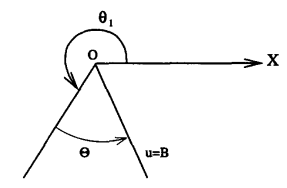
\includegraphics[scale=0.5]{Images/rotated_wedge.png}
        \caption{Rotation of the wedge domain. Image taken from \cite{li2000singularities}.}
        \label{rotated_wedge}
    \end{figure}
    In applications, we are mostly concerned with Dirichlet-Dirichlet, Dirichlet-Neumann and Neumann-Dirichlet boundary conditions. Just like stated above, some of these boundary conditions have different expansions for the angles \(\Theta=\frac{\pi}{2}\) and \(\Theta=\frac{3\pi}{2}\). However, we are only concerned with the expansion
    \[
        v(r,\theta) = \sum_{k=0}^{\infty}\alpha_k r^{\alpha_k}\psi(\alpha_k \theta)
    \]
    where \(\psi=\sin\) or \(\psi = \cos\). In these cases, if we neglect the other terms, for the special angle \(\Theta = \frac{\pi}{2}\) above we would find that \(\alpha_k \in \mathbb{N}\). Without going in dept in singularity analysis, then its partial derivative \(\partial_r v(r,\theta)\) would be of the form 
    \[
        \partial_r v(r,\theta) = \sum_{k=0}^{\infty}\alpha_k^2 r^{\alpha_k-1}\psi(\alpha_k \theta)
    \]
    where \(\alpha_k-1 \in \mathbb{N}\). In general, if \(\alpha_k \in \mathbb{N}\) for some angle \(\Theta\) then all of its derivatives are continuous and \(v(r,\theta)\) is analytical. More precisely, there is no singularity in these cases. Therefore, one does not need to enrich the set of basis functions since the fundamental solutions correctly reproduce the behavior near the corner's tip. Such corners are called \textit{regular}. On the other hand, corners which present singularities are called \textit{singular} and are the ones which we are interested to better approximate. 

    Also notice that, in the expansions above, the term \(r^{-\alpha_k}\) does not appear. This has to do with the fact we are dealing with an interior problem: when considering the exterior problem, the terms \(r^{\alpha_k}\) are replaced with \(r^{-\alpha_k}\) (observe that it satisfies the asymptotic conditions prescribed in order to have well-posedness!).
\end{remark}

To incorporate the singular behavior near a singular corner, first assume, without loss of generality, that the domain \(\Omega\) has just one corner and that the solution of our BVP can be decomposed in regular and singular parts,
\[
    u(x) = u_R(x) + u_S(x), \; x \in \overline{\Omega},
\]
where \(u_R\) is the regular part is approximated by the MFS basis functions, and the singular part \(u_S\) is approximated by the expansions above, having the boundary conditions into account. Let \(\phi_s(r, \theta)\) be one of those expansions centered at the corner's tip, where \(s\) is the order of the expansion. Then, the numerical approximation can be written as
\begin{equation}
    \tilde{u}(x) = \sum_{j=1}^{N}\alpha_j \Phi(x-y_j) + \alpha_{N+1} + \sum_{s=1}^{p} \beta_s \phi_s(r(x),\theta(x)), \; x \in \overline{\Omega}.
\end{equation}
Considering the collocation points \(x_1,\dots,x_M \in \partial \Omega\), the linear system of equations \eqref{mfs_m_system} can be generalized to
\begin{equation}
    {\underbrace{\bigg[ \begin{array}{c | c}
        A_1 & B_1 \\
    \end{array} \bigg]}_{A}}_{M\times(N+1+P)}
    \begin{bmatrix}
        \alpha\\
        \beta
    \end{bmatrix}_{(N+1+P)\times 1}
    =
    \bigg[ \begin{array}{c}
        g \\
    \end{array} \bigg]_{M\times 1},
\end{equation}
where the block matrix \(A_1\) is the matrix \(A\) in \eqref{mfs_m_system} and the \(B_1\) block matrix is given by
\[
    B_1=\begin{bmatrix}
        \phi_1(r(x_1), \theta(x_1)) & \cdots & \phi_p(r(x_1), \theta(x_1)) \\
        \vdots & \ddots & \vdots\\
        \phi_1(r(x_M), \theta(x_M)) & \cdots & \phi_p(r(x_M), \theta(x_M)).
    \end{bmatrix}
\]


\section{Numerical approach for the Helmholtz Equation}
For the Helmholtz equation, the MFS convergence and stability results resemble the previous ones for the Laplace equation with Dirichlet boundary conditions. Once again, the results are stated for identical geometries as before, where \(\Omega\) is the unit disk and the radius of \(\hat{\Omega}\) is \(R>1\). Here is assumed that the boundary data \(g\) can be analytically extended to the annulus \(\{z \in \mathbb{C}: \frac{1}{\rho}< \abs{z} < \rho\}\), where \(\rho > 1\). The following result is due to \cite{barnett2008stability}.
\begin{theorem}
    Let \(R > 1\) and \(N\) be an even number. Then the minimum boundary error achieved by the MFS in the unit disk satisfies
    \[
        \norm{g - \tilde{u}_{|\Gamma}}_{L^2(\Gamma)} \leq 
        \begin{cases}
            C \rho^{-\frac{N}{2}}, \text{ if } \rho < R^2\\
            C \sqrt{N} R^{-N}, \text{ if } \rho = R^2\\
            C R^{-N}, \text{ if } \rho > R^2\\
        \end{cases}
    \]
    where \(C\) is a constant that not depends on \(N\).
\end{theorem}
To solve the Helmholtz equation with the MFS, one must start by computing the eigenvalues \(\lambda\) (or the eigenfrequencies \(k\), with \(\lambda = k^2\)) first. In order to achieve that, recall that the Helmholtz equation
\[
    \begin{cases}
        -\Delta u = \lambda u, \text{ in } \Omega\\
        u = 0, \text{ on } \partial \Omega
    \end{cases}
\]
is well-posed when \(\lambda\) is not an eigenvalue, and in that case the nullspace of the single layer potential operator
\[
    S_k \varphi(y) = \int_{\hat{\Gamma}} \Phi_k(x-y)\varphi(x) d\sigma(x) 
\]
is trivial. More precisely, one can prove the following result, e.g. \cite{alves2005method}.
\begin{theorem}\label{mfs_helm_null_kern}
    If \(k\) is not an eigenfrequency of the interior Dirichlet problem, then \(\dim \left(N(S_k)\right)=0\).
\end{theorem}
\begin{proof}
    If \(k\) is not an eigenfrequency, then the interior problem is well posed which implies that \(\varphi(x) = 0, \; x \in \overline{\Omega}\). By analytical continuation, \(\varphi(x) = 0, \; x \in \hat{\Omega}\). Since the single layer potential is continuous, then \(\varphi(x) = 0, \; x \in \hat{\Gamma}\). By the well-posedness of the exterior problem (notice that the single layer potential satisfies the Sommerfeld radiation conditions), then \(\varphi(x) = 0, \; \forall x \in \mathbb{R}^2\).
\end{proof}

This theorem can be used to search for the eigenvalues/eigenfrequencies of the Laplace operator. By virtue of the discretization of the single layer potential \eqref{mfs_approx_disc}, one should find the values \(k\) such that the nullspace of the matrix \(A(k) = \begin{bmatrix}
    \Phi_k(x_i - y_j)
\end{bmatrix}_{M \times N}\) is not trivial. Like it was discussed in the previous section \ref{n_a_mfs_lap}, that can be done in two different ways:
\begin{enumerate}
    \item if \(A(k)\) is a square matrix (with \(M=N\)), one can compute the determinant of \(A(k)\). Since the components of \(A(k)\) are complex numbers, then its determinant is also a complex number, and we consider its absolute value. In any case, instead of working with \(\abs{\determinant A(k)}\), since this value is very small, one must work with its logarithm and consider the function \(d(k) = \log \abs{\determinant A(k)}\);
    \item if \(A(k)\) is an \(M\times N\) rectangular matrix, with \(M > N\), one considers the smallest singular value, which we denote by \(\sigma_N(k)\), where the singular values of \(A(k)\) are assumed to be in decreasing order \(\sigma_1(k) \geq \dots \geq \sigma_N(k)\). We emphasize that we only work with this case.
\end{enumerate}
Therefore, in order to find the eigenvalues/eigenfrequencies of the Laplace operator, one must find the singularities of the functions \(d(k)\) or \(\sigma_N(k)\) for the first and second cases above, respectively.

\subsection{The Subspace Angle Technique}

Again, one of the drawbacks of this method is the ill-conditioning of the system. In this subsection we introduce the so-called \textit{Subspace Angle Technique}, first presented in \cite{betcke2005reviving}. Intuitively, there are two problems at play: firstly, while the MFS only needs the boundary data to approximate the solution of the BVP, the exponential growth of the condition number against the exponential convergence can be seen has the lack of information given by the collocation points on the boundary, which is not enough to decide if an approximate eigenfunction is spurious; secondly, while we proved the linear independence of the basis functions, in practice the columns of the matrix \(A(k)\) are almost linear dependent if its number is too large (in fact, this is, once again, associated with the distance from the boundary to the artificial boundary).

To solve the first problem, we add additional interior points in order to over determine the system; and for the second problem we construct an orthonormal basis of the column space of \(A(k)\), denoted by \(\mathcal{C}(A(k))\), using the \(QR\) factorization of \(A(k)\). Let \(M_B\) be the number of boundary points and \(M_I\) the number of interior points, such that \(M=M_B+M_I\). Then, by adding some interior points the matrix \(A(k)\) can be extended to
\[
    A(k) = \begin{bmatrix}
        A_B(k)\\
        A_I(k)
    \end{bmatrix},
\]
where the indices \(B\) and \(I\) correspond to the block matrices with the boundary and interior collocation points, respectively. To generate an orthonormal basis of the column space of \(A(k)\), consider the \(QR\) factorization of \(A(k)\), given by \(A(k)=Q(k)R\), where \(Q(k)\) is a unitary complex matrix (i.e., \(Q^\dagger(k) = Q^{-1}(k)\)) and \(R\) is an upper triangular matrix. By partitioning \(Q(k)\) in the boundary and interior collocation points we also have
\begin{equation*}
    Q(k) = \begin{bmatrix}
        Q_B(k)\\
        Q_I(k)
    \end{bmatrix},
\end{equation*}
and each unit vector \(u \in \mathcal{C}(A(k))\) has the form
\begin{equation}\label{sat_qr}
    u = \begin{bmatrix}
        u_B\\
        u_I
    \end{bmatrix} = Q(k)v = \begin{bmatrix}
        Q_B(k)\\
        Q_I(k)
    \end{bmatrix}v
\end{equation}
for some \(v \in \mathbb{R}^2\), \(\norm*{v} = 1\). Assuming homogeneous Dirichlet boundary conditions, we are interested in non-trivial solutions \(v \in \mathbb{R}^2\) to the above problem when \(u \approx 0\) at the boundary, i.e, to solve the constrained minimization problem
\[
    \min_{v \in \mathbb{R}^2, \norm*{v}=1} \norm*{Q_B(k) v}. 
\]
The above problem is easy to solve and has a closed form solution which can be found using Lagrange multipliers. The solution \(\check{v}\) is the right singular vector associated with the smallest singular value \(\sigma_N\) and
\[
    \sigma_N(k) = \norm*{Q_B(k) \check{v}}.
\]
Let \(\check{u} = Q(k) \check{v}\). Taking the norm on both sides of equation \eqref{sat_qr}, one can write
\begin{equation}\label{sat_eq}
    1 = \norm{\check{u}}^2 = \norm{\begin{bmatrix}
        Q_B(k)\\
        Q_I(k)
    \end{bmatrix}\check{v}}^2 = \sigma_N^2(k) + \norm*{Q_I(k) \check{v}}^2.
\end{equation}
Notice how equation \eqref{sat_eq} can be used to eliminate spurious solutions: since \(0 < \sigma_N < 1\), if \(\sigma_N \approx 1\), then \(Q_I(k) \check{v} \approx 0 \implies u_I \approx 0\) which is an incorrect solution (is zero on the interior and does not satisfy the boundary constraints); on the other hand, if \(\sigma_N \approx 0\), then we found an eigenfunction which is small on the boundary points and whose interior is not null.

The name Subspace Angle Technique comes from the fact that \(\sigma_N\) is related with the angle between the subspaces \(\mathcal{C}(A(k))\) and \(\mathcal{G}_0\), the space of vectors that are zero at boundary points\footnote{\(\mathcal{G}_0\) can be seen as the discretization of the functions which satisfy the boundary conditions but not the Helmholtz equation.}. The angle \(\phi(k)=\angle (\mathcal{C}(A(k)), \mathcal{G}_0)\) between both subspaces is defined by
\[
    \cos \phi(k) = \sup_{\substack{u \in \mathcal{C}(A(k)), \, \norm{u}=1 \\ v \in \mathcal{G}_0, \, \norm*{v} = 1}} (u, v),
\]
and one can prove (c.f. \cite{betcke2005reviving}) that
\[
    \sigma_N = \sin \phi(k).
\]
Therefore, the discrete problem has a non-trivial solution (i.e. \(\lambda\) is an eigenvalue of the Laplace Operator) if and only if \(\mathcal{C}(A(k))\) and \(\mathcal{G}_0\) have a non-trivial intersection (i.e. \(\phi(k) = l \pi, \, l \in \mathbb{Z}\)).

\begin{remark}
    While the construction above assumed homogeneous Dirichlet boundary conditions, it can be easily generalized to any type of homogeneous boundary conditions \(\mathcal{B}\) by considering the appropriate \(A\) matrix.
\end{remark}

\begin{remark}
    Neither the enrichment technique nor the Subspace Angle Technique are specific methods only applicable to the Laplace equation and the Helmholtz equation, respectively. They can be used for both equations and at the same time. For example, in \cite{antunes2010meshfree}, both methods were used to study the spectrum of the Laplace operator in domains with corners and cracks.
\end{remark}

% If Printing on DOUBLE SIDED pages, the second page should be white.
% Otherwise, comment the following command:
%\cleardoublepage
%
%Chapter 4
% #############################################################################
% This is Chapter 4
% !TEX root = ../main.tex
% #############################################################################
\fancychapter{Conducted Numerical Simulations}
% \cleardoublepage
\label{chap:implement}

\section{Dirac equation simulations}\label{dirac_equation_simulations}

Recall the system of equations given in \eqref{dirac}
\begin{equation}
    \begin{bmatrix}
        m & -i(\partial_1 - i \partial_2)\\
        -i(\partial_1 + i \partial_2) & -m
    \end{bmatrix}
    \begin{bmatrix}
        u_1(x)\\
        u_2(x)
    \end{bmatrix}
    =\lambda
    \begin{bmatrix}
    u_1(x)\\
    u_2(x)
    \end{bmatrix},
\end{equation}
which can be reduced to the Helmholtz equation with Cauchy-Riemann oblique boundary conditions
\begin{equation*}
    \begin{cases}
        &-\Delta u_1 = (\lambda^2 - m^2)u_1, \; \text{ in } \Omega\\
        & i (\partial_1 + i\partial_2)u_1 + (\lambda + m)i(n_1 + i n_2)u_1 = 0, \; \text{ on } \Gamma,
    \end{cases}      
\end{equation*}
where \(\Gamma = \partial\Omega\) as usual, and the function \(u_2\) depends on the function \(u_1\) by the following equality
\[
    u_2 = \frac{-i (\partial_1 + i\partial_2)u_1}{\lambda + m}.    
\]
\subsection{Numerical validation of the method}

In order to validate the MFS for the Dirac equation with infinite mass boundary conditions, we start by testing it for the unit disk. If \(m=0\), then its value is known like stated in Proposition \ref{dirac_properties}, where \(\lambda_1(\mathbb{D})= 1.434695650819\) is the solution of the equation
\[
    J_0(\lambda_1(\mathbb{D})) = J_1(\lambda_1(\mathbb{D})).
\]

In the numerical simulations presented below, 158 inner collocation points for the subspace angle technique were considered and the number of source points \(N\) is always half of the number of boundary points. Figure \ref{dirak_disk_col_m0} shows the configuration used. The method described at the end of the subchapter \ref{density_proofs_section} was used to place the source points, where \(\eta=0.5\) was used. 

\begin{figure}[!htb]
    \centering
    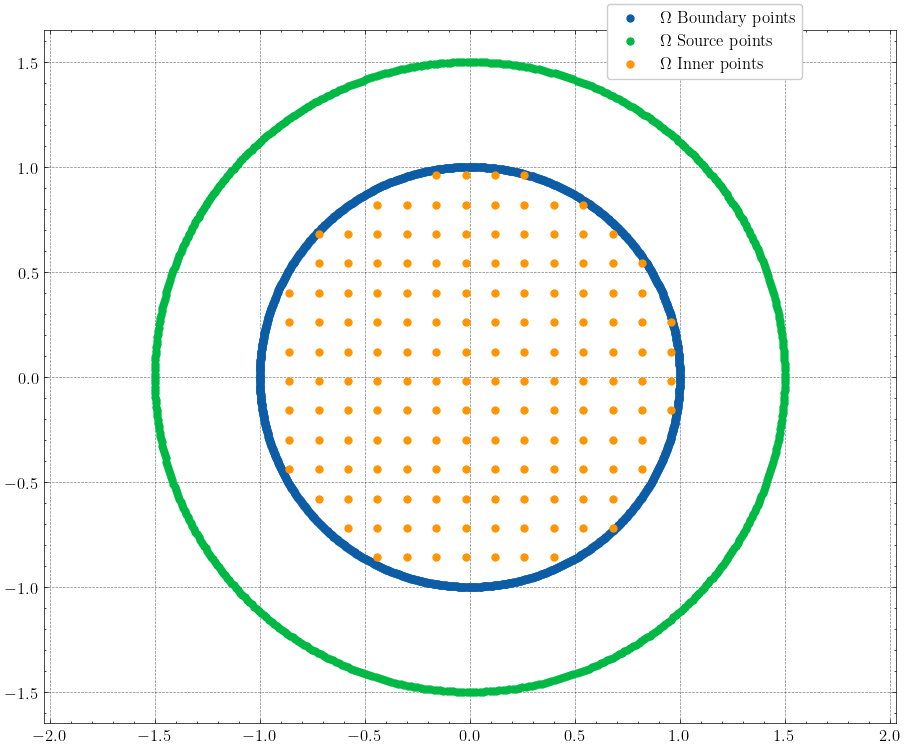
\includegraphics[width=0.5\linewidth]{Images/Dirac/circle_m_0_col_points_158_inner_eta_05.png}
    \captionof{figure}{Configuration of the boundary, source, and inner points. The number of boundary collocation points used is 1200.}
    \label{dirak_disk_col_m0}
\end{figure}

While in the other numerical simulations to be presented more eigenvalues are studied, in Table \ref{tab:eigenvalues_disk_val} only the first three eigenvalues are shown for the sake of brevity.

\begin{table}[htbp]
    \centering
    \begin{tabular}{cccc}
        \toprule
        \textbf{Eigenvalues} & \textbf{N=1200} & \textbf{N=1000} & \textbf{N=800} \\
        \midrule
        \(\tilde{\lambda}_1(\mathbb{D})\) & $1.4346956515$ & $1.4346956481$ & $1.4346956367$ \\
        \(\tilde{\lambda}_2(\mathbb{D})\) & $2.6298741163$ & $2.6298741147$ & $2.6298741276$ \\
        \(\tilde{\lambda}_3(\mathbb{D})\) & $3.1128644920$ & $3.1128645083$ & $3.1128645008$ \\
        \midrule
        \textbf{Absolute error: } \(\abs{\lambda_1(\mathbb{D}) - \tilde{\lambda}_1(\mathbb{D})}\) & $6,877\times 10^{-10}$ & $2,693\times 10^{-9}$ & $1,413\times 10^{-8}$ \\
        \bottomrule
    \end{tabular}
    \caption{Eigenvalues for different values of \(N\) and the measured absolute error.}
    \label{tab:eigenvalues_disk_val}
\end{table}

The plot of the bracketing algorithm \ref{direct_bracketing_algorithm} is shown in Figure \ref{dirac_disk_alg_m0}. For future reference, the first eigenfunction on the disk with \(m=0\) is also shown in Figure \ref{dirac_disk_plots_m0}, where the real and imaginary parts of the spinors \(u_1\) and \(u_2\) are presented. The plots are also normalized, i.e, \(\norm*{\mathbf{u}}_{L^2(\mathbb{D})}=1\).

\begin{figure}[!htb]
    \centering
    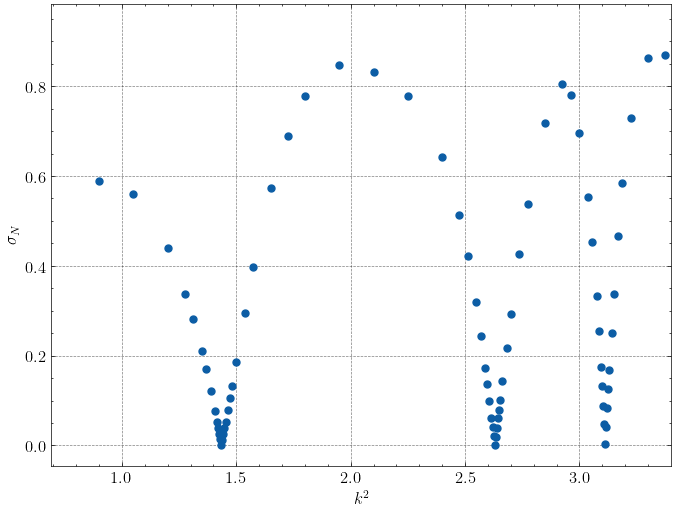
\includegraphics[width=0.5\linewidth]{Images/Dirac/circle_m_0_alg_points_158_inner_eta_05.png}
    \captionof{figure}{Direct search algorithm for the first three eigenvalues of the disk with \(m=0\). Empirically, better approximations are obtained when smaller values of \(\sigma_N\) are found in each singularity.}
    \label{dirac_disk_alg_m0}
\end{figure}

\begin{figure}[!htb]
    \centering
    \begin{minipage}[b]{0.45\textwidth}
        \centering
        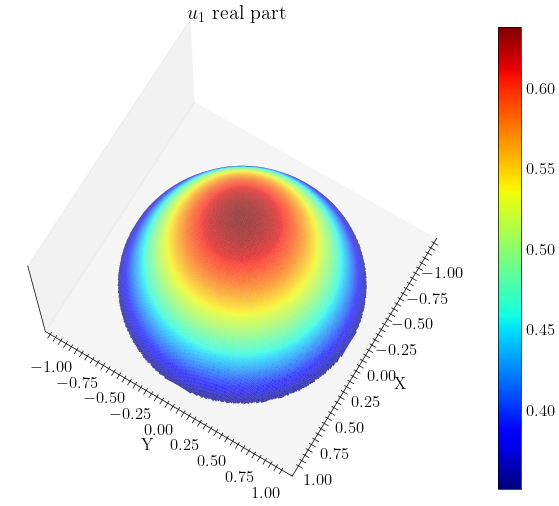
\includegraphics[width=0.8\textwidth]{Images/Dirac/circle_m_0_u1_re_points_158_inner_eta_05.png}
%\caption{Network 1}
    \end{minipage}
    \hfill
    \begin{minipage}[b]{0.45\textwidth}
        \centering
        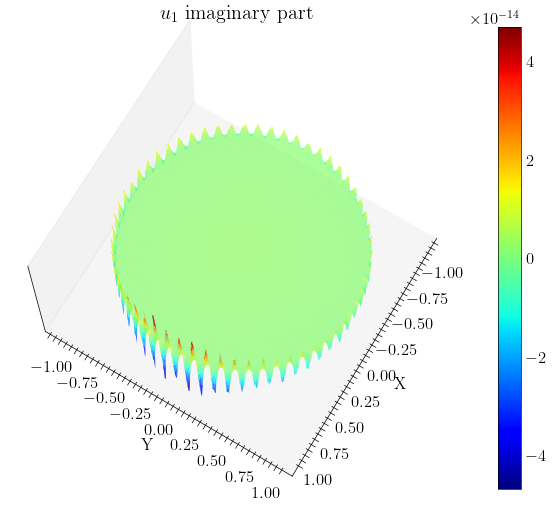
\includegraphics[width=0.8\textwidth]{Images/Dirac/circle_m_0_u1_im_points_158_inner_eta_05.png}
%\caption{Network 2}
    \end{minipage}

    \vspace{0.5cm}

    \begin{minipage}[b]{0.45\textwidth}
        \centering
        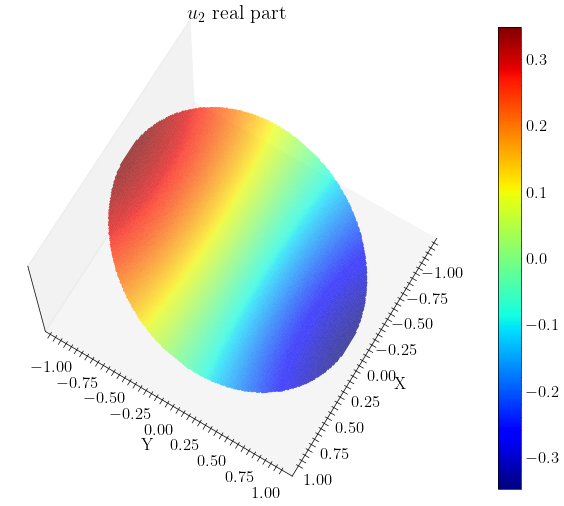
\includegraphics[width=0.8\textwidth]{Images/Dirac/circle_m_0_u2_re_points_158_inner_eta_05.png}
%\caption{Network 3}
    \end{minipage}
    \hfill
    \begin{minipage}[b]{0.45\textwidth}
        \centering
        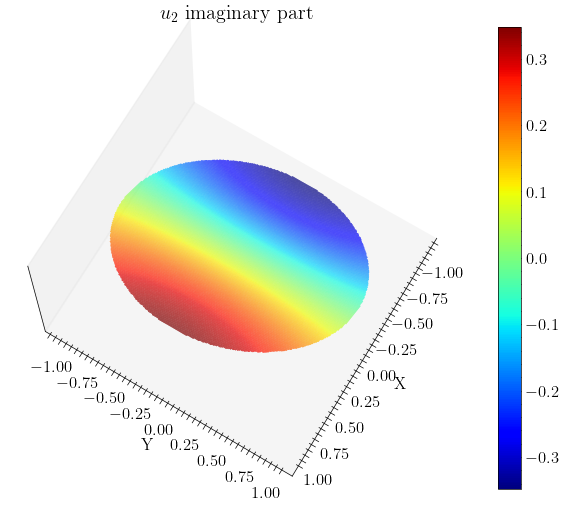
\includegraphics[width=0.8\textwidth]{Images/Dirac/circle_m_0_u2_im_points_158_inner_eta_05.png}
%\caption{Network 4}
    \end{minipage}
    \caption{Plots of the real and imaginary parts of \(u_1\) and \(u_2\) of the first eigenfunction \(\mathbf{u}=\begin{bmatrix} u_1\\ u_2 \end{bmatrix}\). Observe that the imaginary part of \(u_1\) is zero and the artifacts presented are due to precision lost.}
    \label{dirac_disk_plots_m0}
\end{figure}



\subsection{Quadrilateral results}

In this subchapter, several numerical results regarding quadrilateral polygons are shown and discussed. First, numerical evidence for the Conjecture \ref{david_conjectures} is presented both for \(m=1\) and \(m=5\). Then, some simulations show that the conjectured Ashbaugh-Benguria Theorem \ref{conjecture_benguria} also holds for the Dirac operator with infinite-mass boundary conditions. Finally, we will also show that some disagreement between the spectrum of both operators is already evident for the third eigenvalue, whose optimal shape is not the disk, contrary to what is conjectured for the Laplacian (which is still an open problem).

Consider a rectangle with a width \(a > 0\) and unitary area, where the sides are \(a\) and \(\frac{1}{a}\). Figures \ref{eigenvalues_rectangle_width_m_1} and \ref{eigenvalues_rectangle_width_m_5} illustrate the behavior of the first 5 eigenvalues for \(m=1\) and \(m=5\), respectively. Several interesting observations can be made:

\begin{itemize}
  \item The behavior of the spectrum remains qualitatively consistent for different values of \(m\). Notably, the most prominent difference lies in the decreasing gap between the numerical eigenvalues and \(m\) as \(m\) increases. While this trend is discernible, it becomes more apparent as \(m\) takes on even larger values. However, it is important to notice that the third eigenvalue is not globally minimized in the square for \(m=1\), but for some rectangle with width \(a \approx 2.2\). It appears that there exists some critical mass \(m_{\text{crit}}\) between 1 and 5 where that bifurcation occurs. 
  
  \item Starting from the third eigenvalue and beyond, certain spikes become evident in the plot. These spikes correspond to rectangular domains where the eigenvalue has a multiplicity of two. For instance, between the values 1 and 1.5, the third and fourth eigenvalues appear to converge. This behavior becomes more frequent as the order of the eigenvalues increases. However, only multiplicity 2 is observed which is not consistent with the behavior seen in the Laplace operator, where multiplicity 3 is already achieved in the third eigenvalue and only the first eigenvalue is simple;
  
  \item By varying the parameter \(a\), linear growth in the eigenvalues is observed, with no change in their multiplicity. As \(a\) increases, the eigenvalues approach one another, as expected. This phenomenon occurs because the rectangle transforms into an unbounded line, resulting in a non-discrete spectrum.
\end{itemize}

\begin{figure}[!htb]
    \centering
    \begin{minipage}{.5\textwidth}
      \centering
      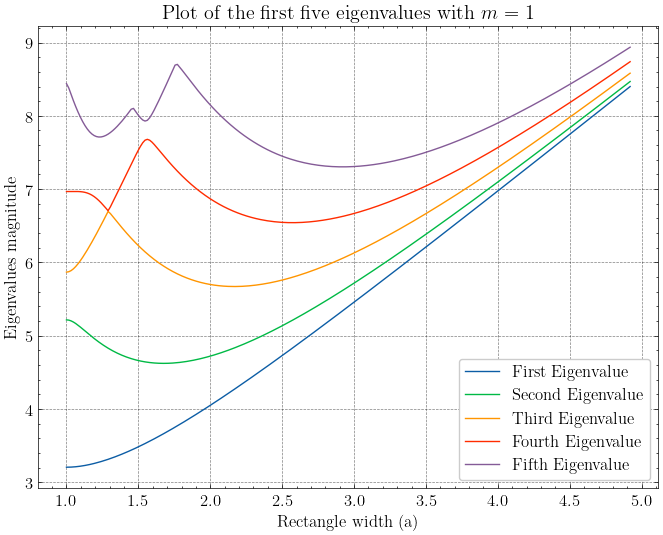
\includegraphics[width=\linewidth]{Images/Dirac/quad/eigenvalues_rectangle_width_m_1.png}
      \captionsetup{width=0.9\linewidth} % Adjust the width of the caption
      \captionof{figure}{Behavior of the first five eigenvalues for rectangles with unit area, width \(a\) and \(m=1\).}
      \label{eigenvalues_rectangle_width_m_1}
    \end{minipage}%
    %\hspace{0.5cm} % Add some horizontal space between the figures
    \begin{minipage}{.5\textwidth}
      \centering
      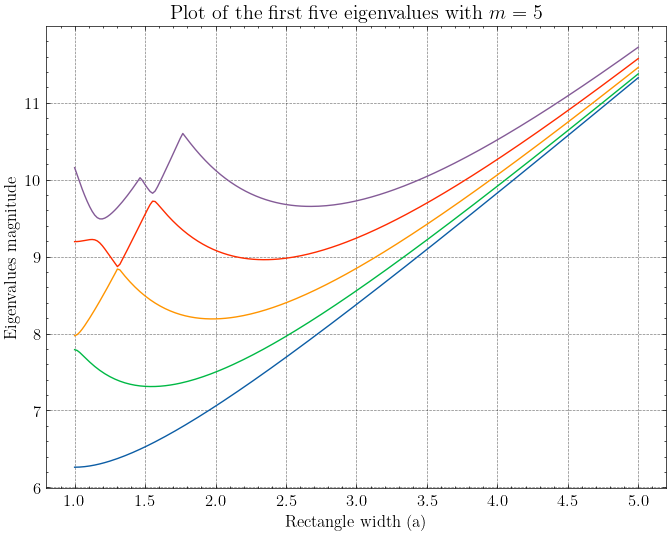
\includegraphics[width=1\linewidth]{Images/Dirac/quad/eigenvalues_rectangle_width_m_5.png}
      \captionsetup{width=0.9\linewidth} % Adjust the width of the caption
      \captionof{figure}{Behavior of the first five eigenvalues for rectangles with unit area, width \(a\) and \(m=5\).}
      \label{eigenvalues_rectangle_width_m_5}
    \end{minipage}
\end{figure}

In Figures \ref{eigenvalues_rectangle_perimeter_width_m_1} and \ref{eigenvalues_rectangle_perimeter_width_m_5} the results for the perimeter are shown. While Conjecture \ref{david_conjectures} is framed for \(a \in (0, 2)\) observe that is enough to consider \(a \in (0, 1)\) given the symmetry of the problem. Here, one considers the perimeter to be 4, and by varying the rectangle width the area is not constant. The conclusions presented earlier are still valid.

\begin{figure}[!htb]
    \centering
    \begin{minipage}{.5\textwidth}
      \centering
      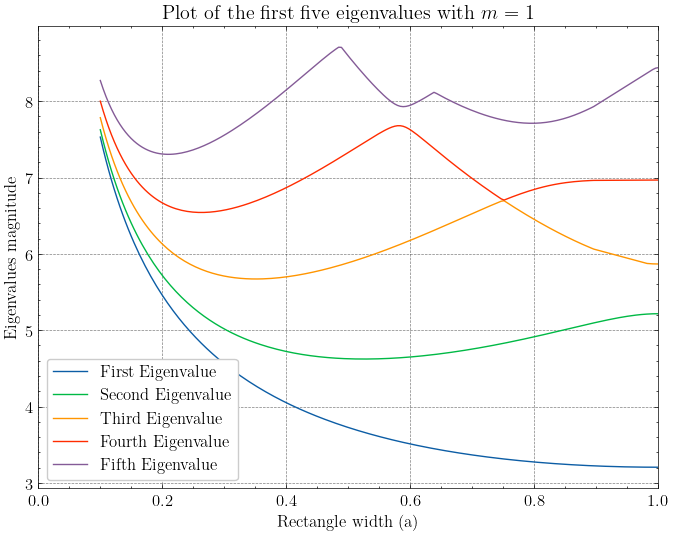
\includegraphics[width=\linewidth]{Images/Dirac/quad/eigenvalues_rectangle_perimeter_width_m_1.png}
      \captionsetup{width=0.9\linewidth} % Adjust the width of the caption
      \captionof{figure}{Behavior of the first five eigenvalues for rectangles with unit area, width \(a\) and \(m=1\).}
      \label{eigenvalues_rectangle_perimeter_width_m_1}
    \end{minipage}%
    %\hspace{0.5cm} % Add some horizontal space between the figures
    \begin{minipage}{.5\textwidth}
      \centering
      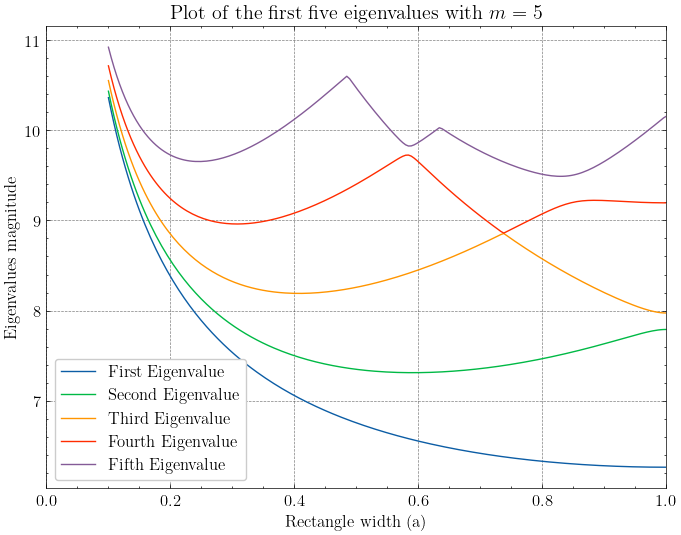
\includegraphics[width=1\linewidth]{Images/Dirac/quad/eigenvalues_rectangle_perimeter_width_m_5.png}
      \captionsetup{width=0.9\linewidth} % Adjust the width of the caption
      \captionof{figure}{Behavior of the first five eigenvalues for rectangles with unit area, width \(a\) and \(m=5\).}
      \label{eigenvalues_rectangle_perimeter_width_m_5}
    \end{minipage}
\end{figure}

Given the results for rectangles with fixed area or perimeter, it is possible to state that the Conjecture \ref{david_conjectures} should hold, although it is still not possible to ascertain that the results presented here hold for every \(m\) (as we saw before, the value of \(m\) has some discernible influence on the spectrum, which can already be seen for the third eigenvalue, although no difference was found for the first and second eigenvalues). In any case, it is known that the eigenvalues are continuous with domain perturbations (here these perturbations can be seen as stretching the rectangles), exactly what has been found in these numerical simulations.

To finish this subchapter, we present the results for general quadrilaterals. Since no (practical) parameterization can describe every quadrilateral, we have resorted to a random sampling of quadrilaterals and studied the results against rectangles and rhombuses. Figure \ref{dirac_first_three_eigenvalues_quad_m_1} presents the results of the numerical simulations for \(m=1\). Notice how the rectangles and rhombuses clearly define a region of ``acceptable'' quadrilaterals and this appears to be particularly true for the first eigenvalue. For the second and third eigenvalues some quadrilaterals behave differently, and it is already possible to find some domains whose third eigenvalue is smaller than the eigenvalue of the unit disk. In Figures \ref{dirac_benguria_quad} and \ref{dirac_generalized_benguria_quad} the ratio between the first eigenvalues is studied, where the version of the Ashbaugh-Benguria Theorem \ref{conjecture_benguria} appears to hold.

\begin{figure}[!htb]
    \centering
    \begin{minipage}[c]{0.8\textwidth}
        \centering
        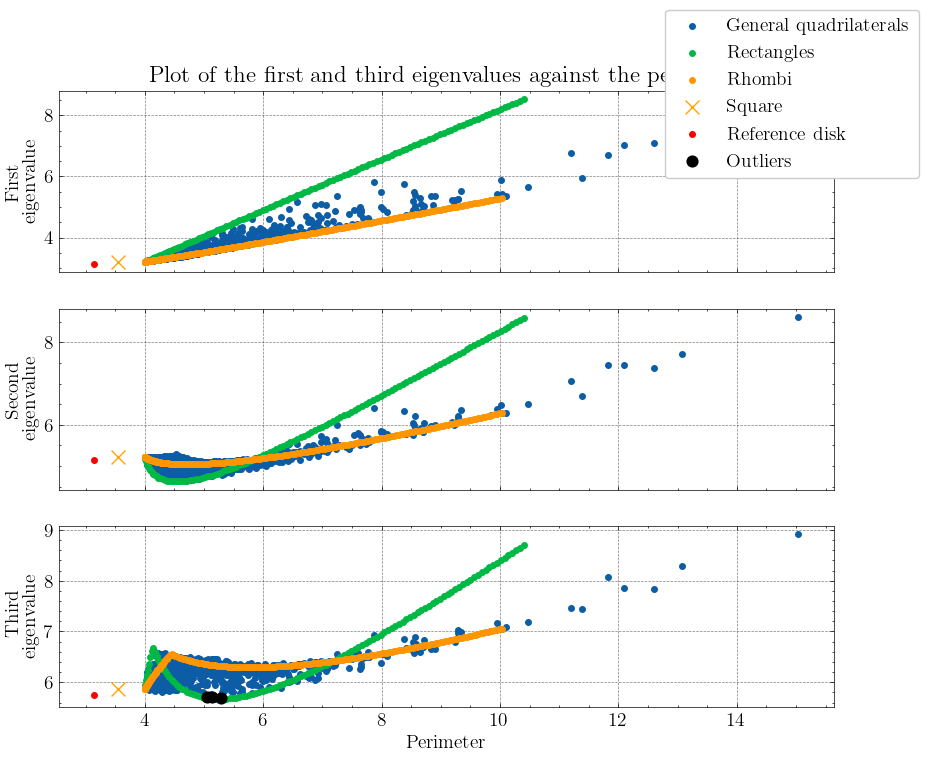
\includegraphics[width=0.8\textwidth]{Images/Dirac/quad/first_three_eigenvalues_quad_m_1.png}
        \caption{Plot of the first three eigenvalues against the perimeter. The ``outliers'' marked in black represent the domains in which the third eigenvalue is less than the third eigenvalue of the disk.}
        \label{dirac_first_three_eigenvalues_quad_m_1}
    \end{minipage}

    \vspace{0.5cm}

    \begin{minipage}[c]{0.45\textwidth}
        \centering
        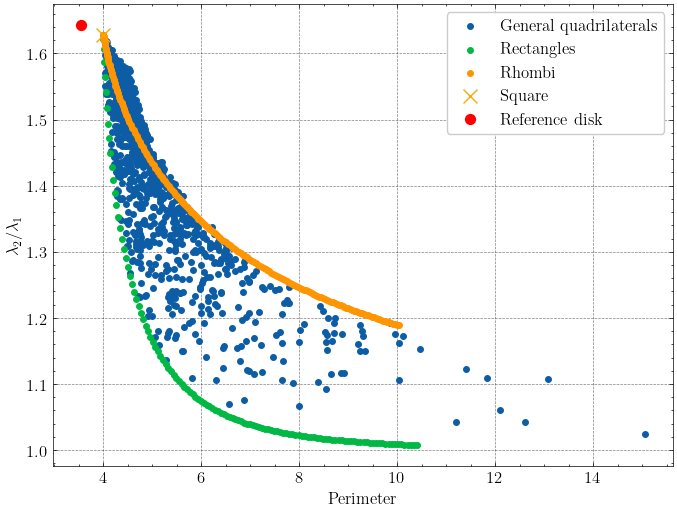
\includegraphics[width=\textwidth]{Images/Dirac/quad/benguria_quad.png}
        \captionsetup{width=0.8\linewidth} % Adjust the width of the caption
        \caption{Ratio between the first two eigenvalues \(\frac{\lambda_2}{\lambda_1}\).}
        \label{dirac_benguria_quad}
    \end{minipage}
    \hfill
    \begin{minipage}[c]{0.45\textwidth}
        \centering
        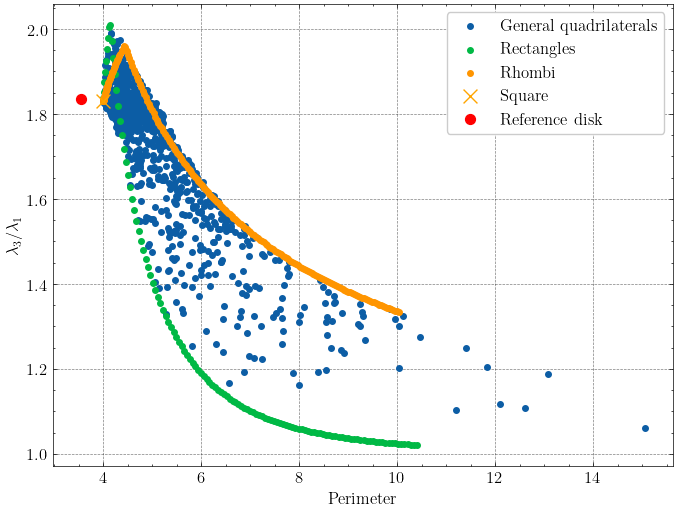
\includegraphics[width=\textwidth]{Images/Dirac/quad/generalized_benguria_quad.png}
        \captionsetup{width=0.8\linewidth} % Adjust the width of the caption
        \caption{Ratio between the third and first eigenvalues \(\frac{\lambda_3}{\lambda_1}\).}
        \label{dirac_generalized_benguria_quad}
    \end{minipage}
    \vspace{0.5cm}
\end{figure}

\subsection{Triangle results}

In this subchapter, we tackle the Conjectures \ref{triangle_conjectures} stated on \cite{vu2023spectral}. Instead of considering random triangles, its study can be done systematically given that, up to congruence, three parameters completely define every triangle. The approach presented here is based on the work of Antunes \& Freitas \cite{antunes2011inverse}. Consider the region \(R\) defined by
\[
    R = \{(x, y) \in \mathbb{R}^2: x \geq 0, y > 0, (x+1)^2 + y^2 \leq 4\},
\]
and its piecewise boundary \(\partial R = \Gamma_0 \cup \Gamma_1 \cup \Gamma_2\), where
\begin{align*}
    \Gamma_0 &= \{(x,y) \in \mathbb{R}^2: 0 \leq x \leq 1, y=0\}\\
    \Gamma_1 &= \{(x,y) \in \mathbb{R}^2: 0 \leq x < 1, y=\sqrt{4-(x+1)^2}\}\\
    \Gamma_2 &= \{(x,y) \in \mathbb{R}^2: x=0, 0 < y < \sqrt{3}\}.
\end{align*}
A triangle \(T\) is said to be \textit{admissible} if its basis vertices are \((0, 0)\) and \((1, 0)\), and the other vertex coordinates\footnote{Of course, one does not need to enforce such constraints to the triangle: as said before, every triangle is unique up to congruence. Here, we just emphasize that is enough to consider triangles defined using the region \(R\). Observe that this is just a model to numerically exhaust all possible triangles up to congruence, one still needs to normalize them to have a unitary area.} are \((x,y)\) such that \((x,y) \in \overline{R}\). A triangle \(T\) is said to be \textit{subequilateral} if \((x, y) \in \Gamma_1\) and \textit{superequilateral} if \((x, y) \in \Gamma_2\); if \((x, y) = (0, \sqrt{3})\) then it is equilateral (obviously). The plot of the region \(R\) and its boundary \(\partial R\) is in Figure \ref{dirac_triangle_model}.
\begin{figure}[!htb]
    \centering
    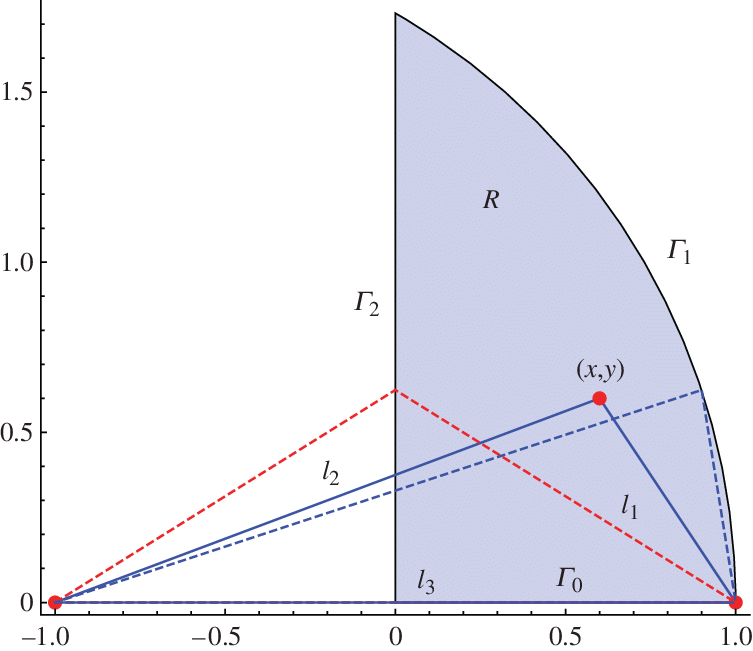
\includegraphics[width=0.5\linewidth]{Images/Dirac/model_triangle.png}
    \captionof{figure}{Configuration space of the admissible triangles. In a dashed red line is a superequilateral triangle; in a dashed blue line a subequilateral triangle is also represented.}
    \label{dirac_triangle_model}
\end{figure}
In Figure \ref{dirac_smooth_first_eigenvalues} we present numerical evidence for Conjecture \ref{triangle_conjectures} with \(m=1\). Notice how the eigenvalues of the superequilateral and subequilateral triangles define a region that includes every other triangle whose \((x, y)\) vertex belongs to \(R\). In Figure \ref{dirac_triangle_benguria} a version of the Ashbaugh-Benguria (see Conjecture \ref{conjecture_benguria}) inequality is presented and in Figure \ref{dirac_triangle_3d_lambda1} a 3D plot of the first eigenvalue for every admissible triangle considered against the coordinates \((x,y)\) of the vertex in \(\overline{R}\).

\begin{figure}[!htb]
    \centering
    \begin{minipage}[c]{0.8\textwidth}
        \centering
        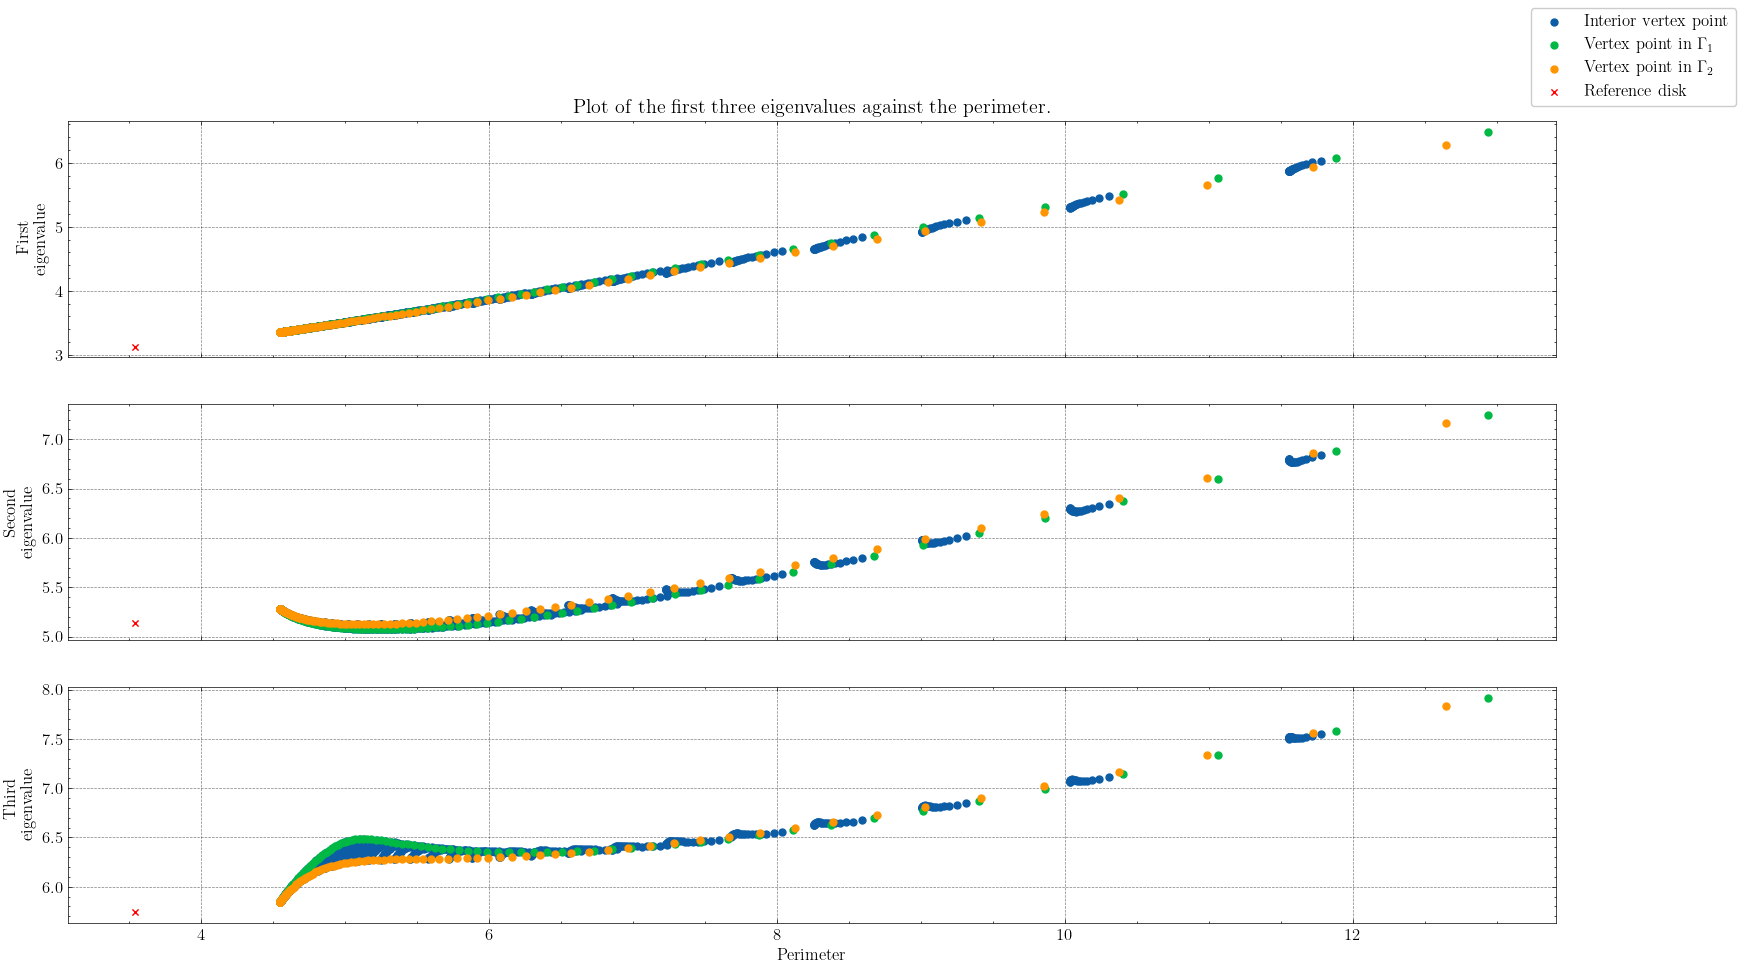
\includegraphics[width=\textwidth]{Images/Dirac/triangles/triangle_first_eigenvalues.png}
        \caption{Plot of the first three eigenvalues against the perimeter. The ``outliers'' marked in black represent the domains in which the third eigenvalue is less than the third eigenvalue of the disk.}
        \label{dirac_smooth_first_eigenvalues}
    \end{minipage}

    \vspace{0.5cm}

    \begin{minipage}[c]{0.41\textwidth}
        \centering
        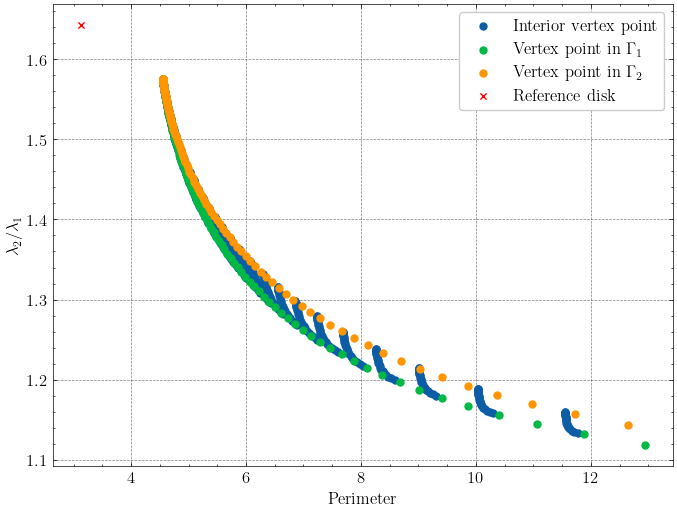
\includegraphics[width=\textwidth]{Images/Dirac/triangles/triangle_benguria.png}
        \captionsetup{width=0.8\linewidth} % Adjust the width of the caption
        \caption{Ratio between the first two eigenvalues \(\frac{\lambda_2}{\lambda_1}\).}
        \label{dirac_triangle_benguria}
    \end{minipage}
    \hfill
    \begin{minipage}[c]{0.50\textwidth}
        \centering
        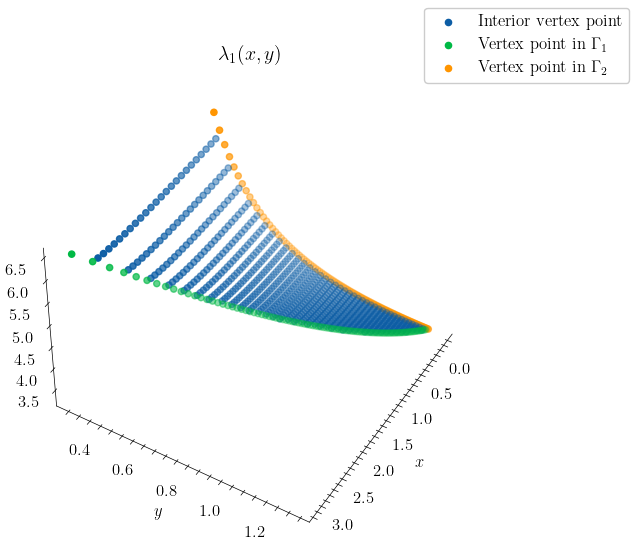
\includegraphics[width=\textwidth]{Images/Dirac/triangles/triangle_3d_lambda1.png}
        \captionsetup{width=0.8\linewidth} % Adjust the width of the caption
        \caption{Ratio between the third and first eigenvalues \(\frac{\lambda_2}{\lambda_1}\).}
        \label{dirac_triangle_3d_lambda1}
    \end{minipage}
    \vspace{0.5cm}
\end{figure}

While in the previous results for quadrilaterals (and for smooth domains in the next subchapter) random domains were considered, it is remarkable that for the triangle problem, one can consider \textit{every} type of triangle just by varying \((x,y)\) in \(\overline{R}\). Since the eigenvalues are continuous when considering domain perturbations, it means that it is very unlikely that the conjectures studied for triangles do not hold, otherwise some jump would probably be found, for example in Figure \ref{dirac_triangle_3d_lambda1}. 


\subsection{Smooth domain results}

In this last subchapter, the behavior of the spectrum for smooth (connected) domains with unit area is studied. Here, we fix \(m=1\). The objective of this study is twofold: first, these type of domains is studied since the numerical approximations are more reliable, and it allows for the study of arbitrary domains; second, one can use them to also study the domain which minimizes the third eigenvalue.

In order to generate random smooth domains, periodic B-spline interpolation for each component of an \(\mathbb{R}^2\) vector was used. One starts by generating five random points (using a uniform distribution), fitting a periodic B-spline in each component, drawing the two-dimensional B-spline, and checking for auto-intersections. If it does not auto-intersect, then it is a valid domain. Figure \ref{dirac_smooth_random_domain} presents one of these domains.

\begin{figure}[!htb]
    \centering
    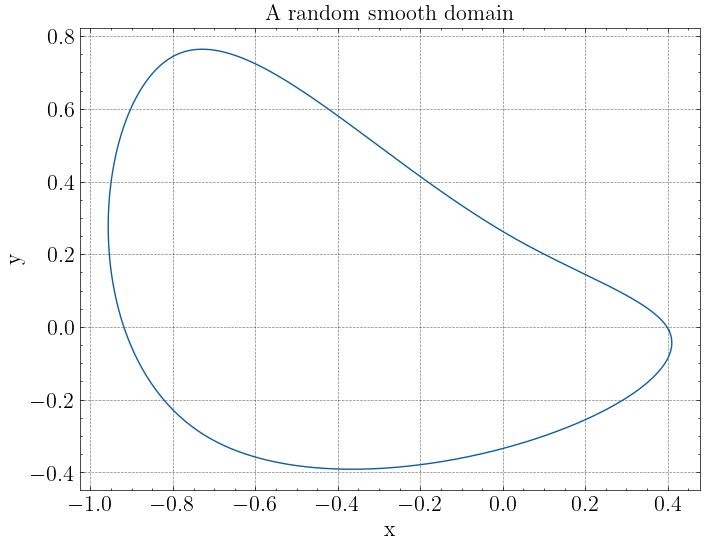
\includegraphics[width=0.55\linewidth]{Images/Dirac/smooth/random_smooth_domain.png}
    \captionof{figure}{Some smooth domain generated by B-splines.}
    \label{dirac_smooth_random_domain}
\end{figure}

The figures below are analogous to the ones presented before. In Figure \ref{dirac_smooth_domains_scatter_all_eigs} a scatter plot of the first three eigenvalues as a function of the perimeter. Once again, analogously to the Laplacian, a Faber-Krahn type result appears to hold for the Dirac operator with infinite-mass boundary conditions. As we saw before, some ``outlier'' domains have a third eigenvalue that is smaller than the third eigenvalue on the disk, which contradicts the conjecture for the Laplace operator.
Figures \ref{dirac_smooth_domains_scatter_benguria} and \ref{dirac_smooth_domains_scatter_benguria_third} are related to the ratio of the first eigenvalues and the spectral gap between them. An analogous to the Ashbaugh-Benguria Theorem for the Laplacian also seems to hold for the Dirac operator, as well its generalization for the ratio \(\frac{\lambda_3}{\lambda_1}\).

\begin{figure}[!htb]
    \centering
    \begin{minipage}[c]{0.8\textwidth}
        \centering
        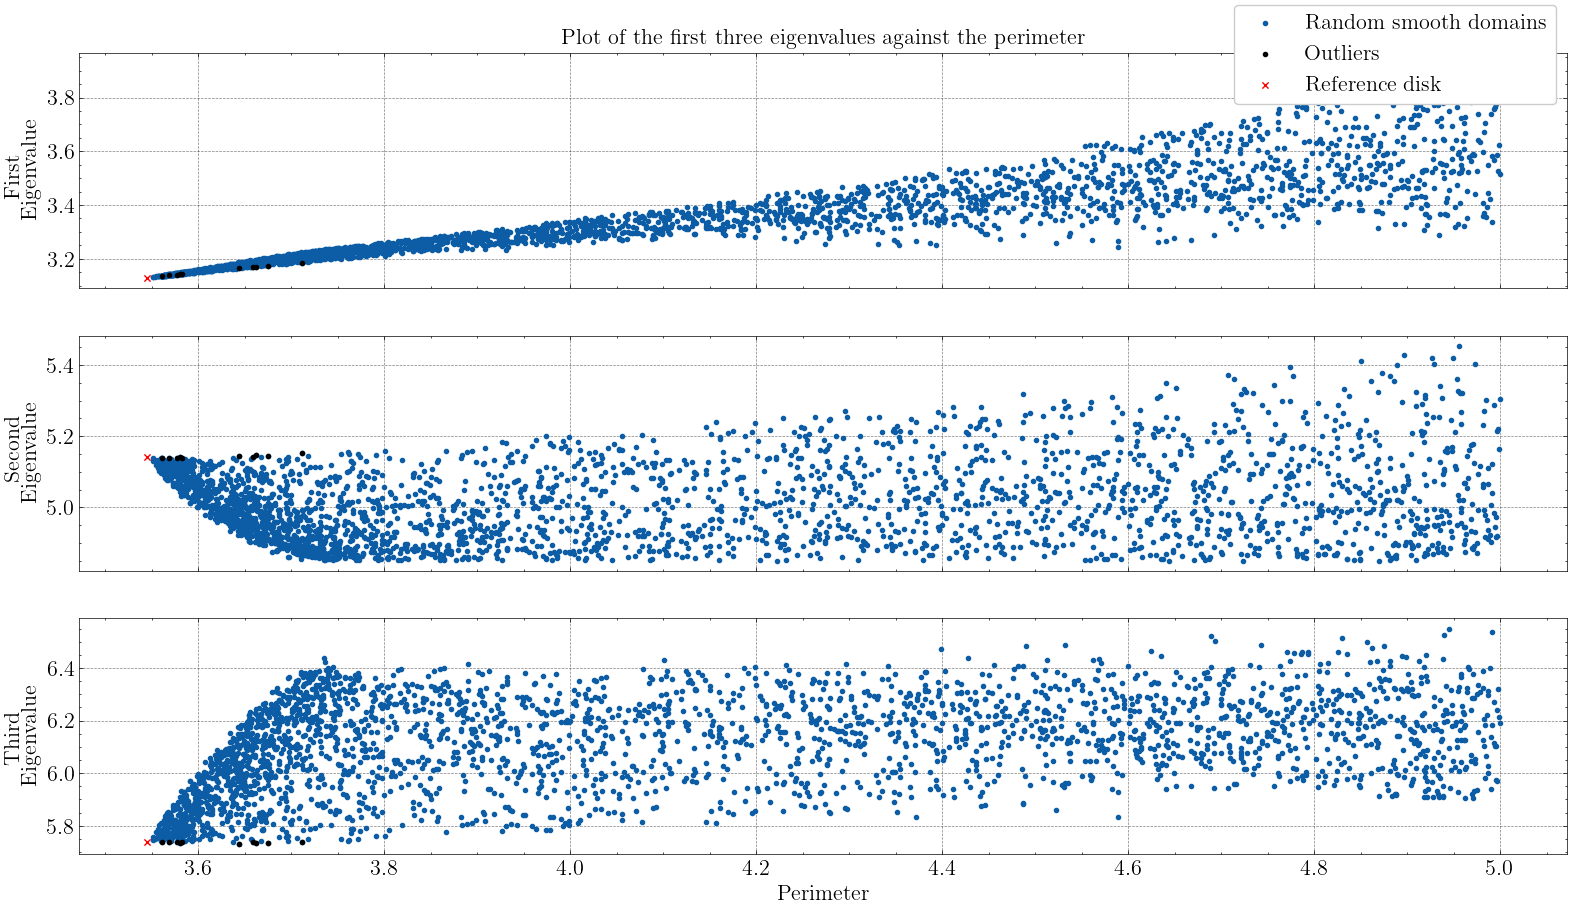
\includegraphics[width=\textwidth]{Images/Dirac/smooth/smooth_domains_scatter_all_eigs_.png}
        \caption{Plot of the first three eigenvalues against the perimeter. The ``outliers'' marked in black represent the domains in which the third eigenvalue is less than the third eigenvalue of the disk.}
        \label{dirac_smooth_domains_scatter_all_eigs}
    \end{minipage}

    \vspace{0.5cm}

    \begin{minipage}[c]{0.45\textwidth}
        \centering
        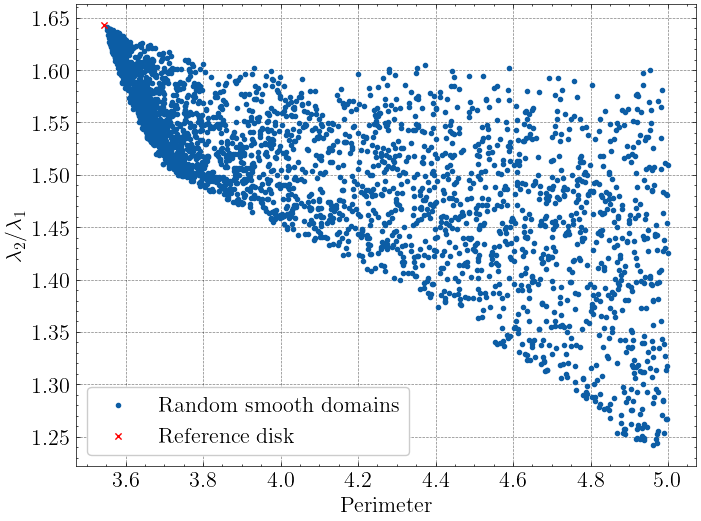
\includegraphics[width=\textwidth]{Images/Dirac/smooth/smooth_domains_scatter_benguria.png}
        \caption{Ratio between the first two eigenvalues \(\frac{\lambda_2}{\lambda_1}\).}
        \label{dirac_smooth_domains_scatter_benguria}
    \end{minipage}
    \hfill
    % \begin{minipage}[c]{0.32\textwidth}
    %     \centering
    %     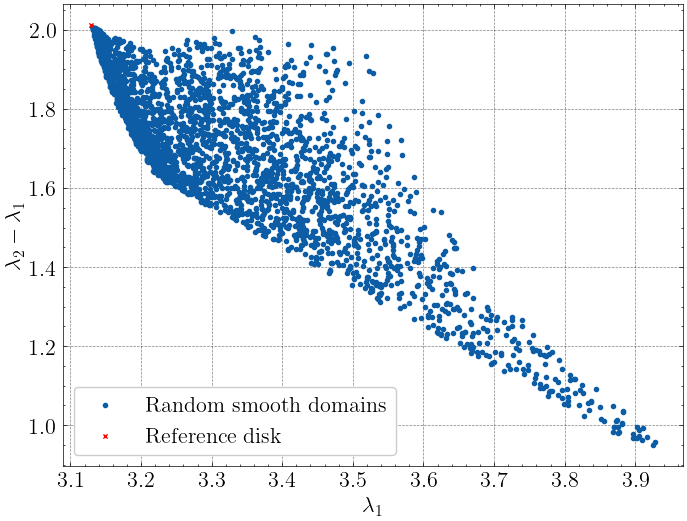
\includegraphics[width=\textwidth]{Images/Dirac/smooth/smooth_domains_scatter_gap.png}
    %     \caption{Spectral gap \(\lambda_2-\lambda_1\).}
    %     \label{dirac_smooth_domains_scatter_gap}
    % \end{minipage}
    % \hfill
    \begin{minipage}[c]{0.45\textwidth}
        \centering
        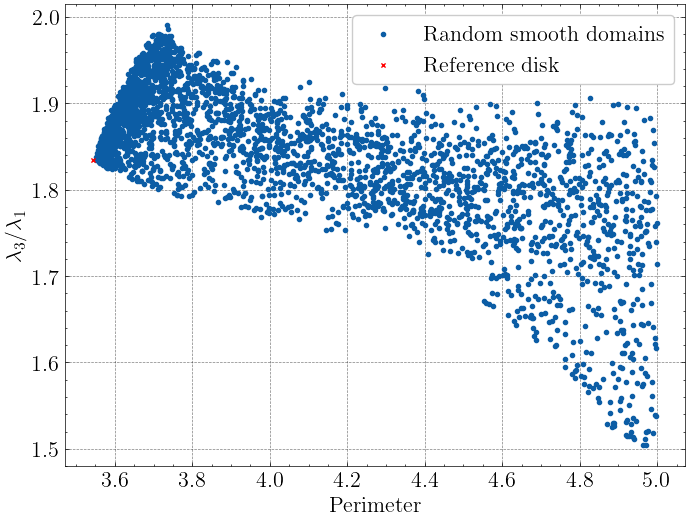
\includegraphics[width=\textwidth]{Images/Dirac/smooth/smooth_domains_scatter_benguria_third.png}
        \caption{Ratio between the third and first eigenvalues \(\frac{\lambda_3}{\lambda_1}\).}
        \label{dirac_smooth_domains_scatter_benguria_third}
    \end{minipage}
\end{figure}

Next, we investigate the domain with the smallest third eigenvalue, and we look for the minimizer of the functional
\begin{equation*}%\label{dirac_min_third_func}
    \mathcal{F}(\Omega) = \lambda_3(\Omega).
\end{equation*}

In general, one can address minimization problems in Banach spaces using the notion of \textit{Fréchet}-derivative. In shape optimization problems, for the eigenvalues of an elliptic operator, one can use the variational formula for its eigenvalues. For example, the formula proved in Theorem \ref{spec_lap_pre} can be used to derive some results for the Laplacian Dirichlet problem. In fact, consider \(\Omega_t = \varphi(t)(\Omega)\) a small perturbation of \(\Omega\) in the parameter \(t\), where \(\varphi(t)\) is some diffeomorphism for small values of \(t\), 
\[
    \varphi(t) = I + t V
\]
for some fix vector field \(V\) and \(\Omega_0 = \Omega\). Let  \(\lambda_k(t)\) be an eigenvalue of the Laplace operator with Dirichlet boundary conditions on the domain \(\Omega_t\) and \(u^{(k)}_t\) its associated eigenfunction in \(H^1_0(\Omega_t)\). If \(\lambda_k\) has multiplicity one (if it is simple) and \(\Omega\) is of class \(C^2\) or convex, then
\[
    \lambda'_k(0) =- \int_{\partial\Omega} \left(\frac{\partial u^{(k)}_0}{\partial n}\right)^2 V\cdot n d \sigma.
\]
For more details, we point the reader to \cite{henrot2006extremum} and \cite{kato2013perturbation}.
As of the moment of writing, the author is not aware of any closed form for the derivative of the eigenvalues of the Dirac operator. In that case, two different strategies were considered to solve the unconstrained minimization problem
\begin{equation}\label{dirac_unconstrained_min_lambda_3}
    \min_{\substack{\Omega \subset \mathbb{R}^2 \\ \abs{\Omega}=1}} \mathcal{F}(\Omega).
\end{equation}

Starting from a given domain \(\Omega\), \(\mathcal{F}\) can be minimized using the \ac{BFGS} algorithm, a quasi-Newton method that uses the local curvature of \(\mathcal{F}\) to find the descent direction given by an approximation of the Hessian matrix. Unfortunately, the \ac{BFGS} method also needs the derivative at the point, which can only be numerically found using finite-difference methods. The second method is the multidimensional Nelder-Mead direct search method. Just like the bracketing algorithm used to find the singularities on the graph of the smallest singular value, the Nelder-Mead method does not use any information on the derivative and relies on evaluations of the loss function \(\mathcal{F}\) to bracket the local minima: in this case, a heuristic strategy with a multidimensional simplex is used to approximate it.

To apply both the \ac{BFGS} and the Nelder-Mead algorithms, one starts by approximating the domain \(\Omega_0\) with the lowest third eigenvalue by a polar parameterization. This is achieved by considering a sample of \(N\) boundary points from the domain, considering its polar coordinates, and finding the coefficients of the trigonometric interpolation. More precisely, let \(M\) be the order of the trigonometric interpolation. Assume that the radial part of each boundary point of \(\Omega_0\) can be parametrized by \(r(\theta)\), where \(\theta \in (0, 2\pi)\). In that case, one uses the approximation
\[
    r(\theta_i) \approx a_0 + \sum_{m=1}^{M}a_m \cos(m \theta_i) + \sum_{m=1}^{M}b_m \sin(m \theta_i),
\]
where \(\theta_i\) is the polar part of the sample point \(i\) with \(i=1,\dots,N\). Then, the system
\[
    \begin{bmatrix}
        1 & \cos(1 x_1) & \cos(2 x_1) & \dots & \cos(M x_1) & \sin(1 x_1) & \dots & \sin(M x_1)\\
        \vdots & \vdots & \vdots & \vdots & \vdots & \vdots & \vdots & \vdots\\
        1 & \cos(1 x_N) & \cos(2 x_N) & \dots & \cos(M x_N) & \sin(1 x_N) & \dots & \sin(M x_N)
    \end{bmatrix}_{N\times(2M+1)}
    \begin{bmatrix}
        a_0\\
        \vdots\\
        b_M
    \end{bmatrix}
    =
    \begin{bmatrix}
        r(\theta_1)\\
        \vdots\\
        r(\theta_N)\\
    \end{bmatrix}
\]
can be solved by least squares when considering the over-determined system with \(N > 2M+1\). Notice that the problem \eqref{dirac_unconstrained_min_lambda_3} is now discretized into a finite-dimensional problem since every domain is now a vector of coefficients in \(\mathbb{R}^{2M+1}\). Of course, one must still consider the domain generated by the found coefficients with unitary area.

Figure \ref{dirac_nelder_mead_domain} presents an (almost) optimal domain \(\Omega^\star\) shape which minimizes the third eigenvalue of the Dirac operator with infinite-mass boundary conditions. This plot was obtained through the Nelder-Mead algorithm. The third eigenvalue of this domain is approximately \(\lambda_3 \approx 5.63787728\) and its perimeter \(L\) is \(L \approx 5.2650031\). In Figure \ref{dirac_val_third} we validate our findings by plotting the (continuous) family of one-parameter transformations (known as a Minkowski sum) from the unit disk to \(\Omega^\star\), given by
\[
   \Omega_t = (1-t)\mathbb{D} + t \Omega^\star, \; 0 \leq t \leq 1.
\]
\begin{figure}[!htb]
    \centering
    \begin{minipage}{.5\textwidth}
        \centering
        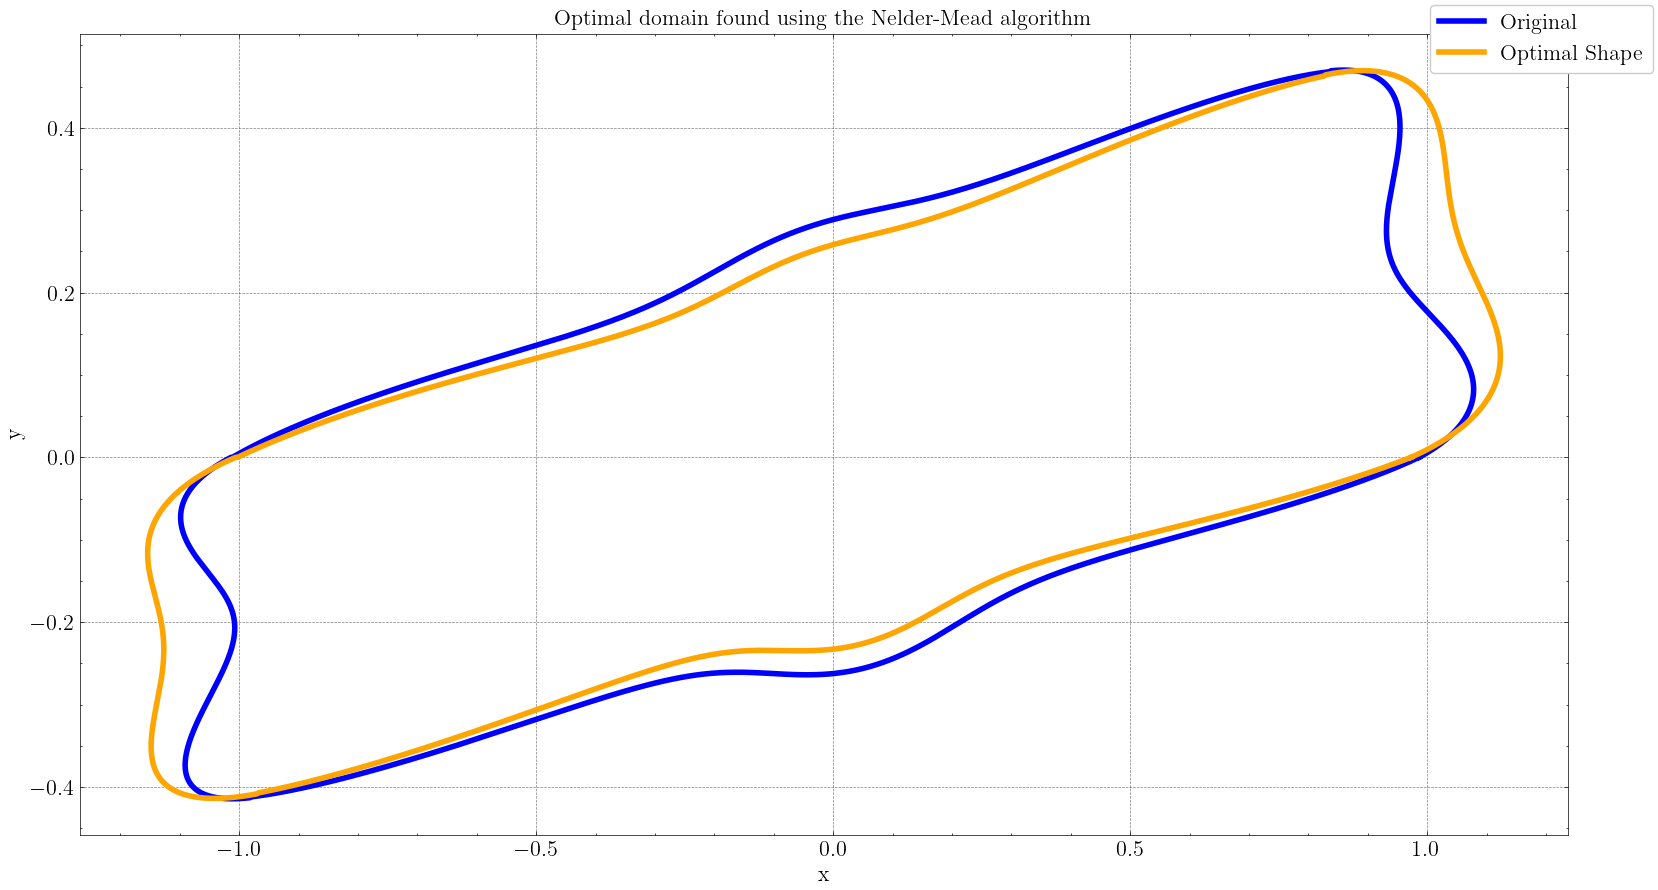
\includegraphics[width=1\linewidth]{Images/Dirac/smooth/nelder_mead_optimal.png}
        \captionsetup{width=0.8\linewidth} % Adjust the width of the caption
        \captionof{figure}{Optimal domain \(\Omega^\star\) (on orange) against the original domain in the first iteration of the Nelder-Mead algorithm.}
        \label{dirac_nelder_mead_domain}
    \end{minipage}%
    \hfill
    %\hspace{0.5cm} % Add some horizontal space between the figures
    \begin{minipage}{.5\textwidth}
        \centering
        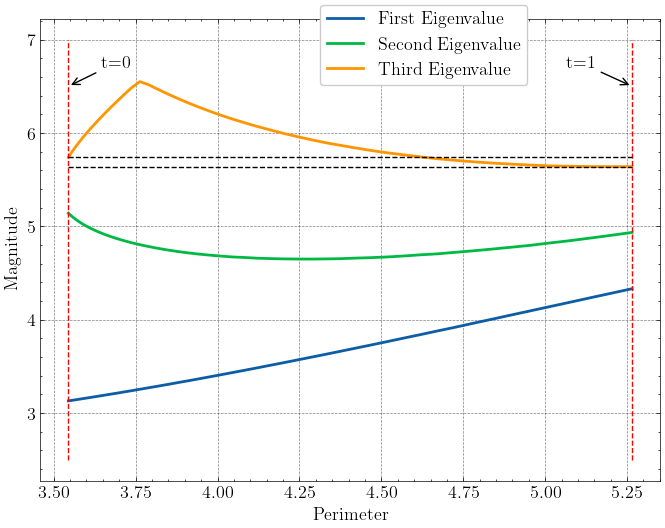
\includegraphics[width=0.9\linewidth]{Images/Dirac/smooth/dirac_val_third.png}
        \captionsetup{width=0.8\linewidth} % Adjust the width of the caption
        \captionof{figure}{Plot of the first three eigenvalues of the Minkowski sum \(\Omega_t\) for each increasing value of \(t\).}
        \label{dirac_val_third}
    \end{minipage}
\end{figure}

As said above, the \ac{BFGS} method was also used. However, no meaningful results were found using this method, since any descent direction produced not  

\begin{remark}
    One can not fail to point out a valid criticism of this method: since we only parametrized the radial part of the domain's boundary, given the periodicity of the trigonometric interpolation one always end up with star-like shapes. Particularly, in our case, the order of the trigonometric interpolation was low, with \(M=4\). However, by increasing the order of interpolation the dimension of the optimization space would increase, and, in this case, we are already working on \(\mathbb{R}^9\), and is very hard for a direct search method like Nelder-Mead to find a local minimum in such a ``high'' dimensional space. The option to only work with the radial part, instead of both cartesian components, was also a way to reduce the dimensionality of the problem. 
\end{remark}

Finally, the normalized eigenfunction associated with the optimal third eigenvalue of domain \(\Omega^\star\) is shown in Figure \ref{dirac_optimal_plots_eigenfunctions}.

\begin{figure}[!htb]
    \centering
    \begin{minipage}[b]{0.45\textwidth}
        \centering
        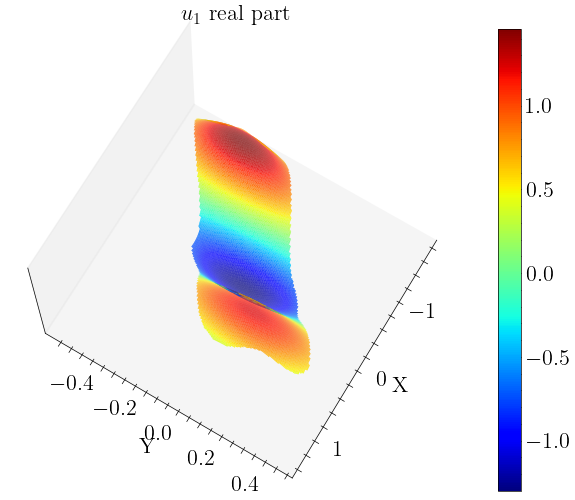
\includegraphics[width=0.8\textwidth]{Images/Dirac/smooth/optimal_lambda3_m_1_u1_re.png}
%\caption{Network 1}
    \end{minipage}
    \hfill
    \begin{minipage}[b]{0.45\textwidth}
        \centering
        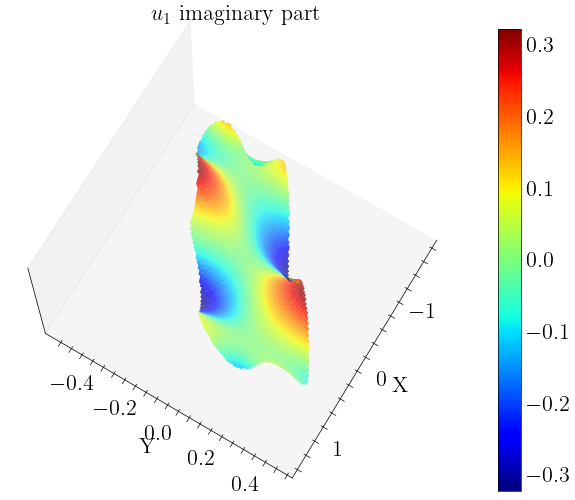
\includegraphics[width=0.8\textwidth]{Images/Dirac/smooth/optimal_lambda3_m_1_u1_im.png}
%\caption{Network 2}
    \end{minipage}

    \vspace{0.5cm}

    \begin{minipage}[b]{0.45\textwidth}
        \centering
        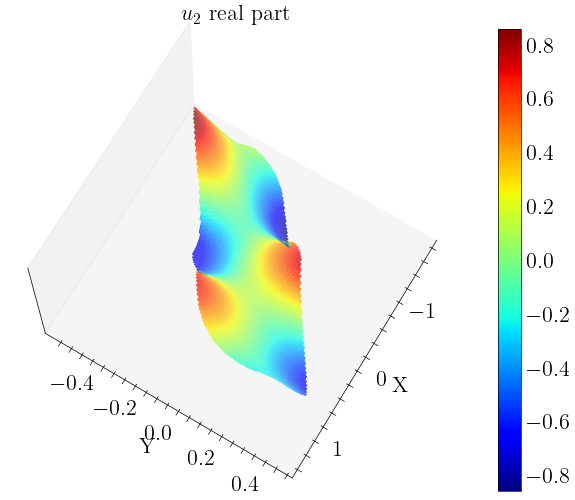
\includegraphics[width=0.8\textwidth]{Images/Dirac/smooth/optimal_lambda3_m_1_u2_re.png}
%\caption{Network 3}
    \end{minipage}
    \hfill
    \begin{minipage}[b]{0.45\textwidth}
        \centering
        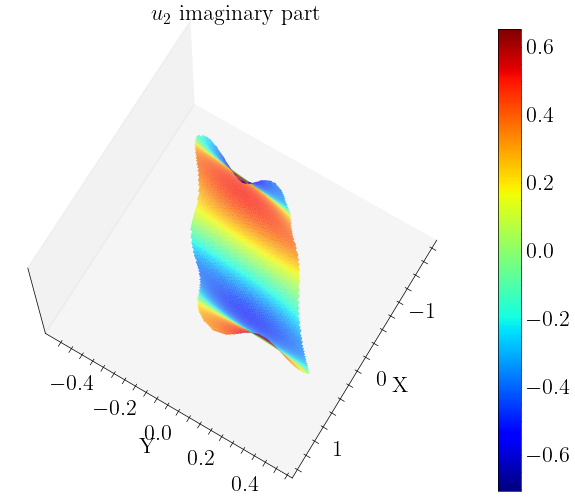
\includegraphics[width=0.8\textwidth]{Images/Dirac/smooth/optimal_lambda3_m_1_u2_im.png}
%\caption{Network 4}
    \end{minipage}
    \caption{Plots of the real and imaginary parts of \(u_1\) and \(u_2\) of the third eigenfunction \(\mathbf{u}=\begin{bmatrix} u_1\\ u_2 \end{bmatrix}\) associated with the optimal domain \(\Omega^\star\).}
    \label{dirac_optimal_plots_eigenfunctions}
\end{figure}

% \begin{figure}[!htb]
%     \centering
%     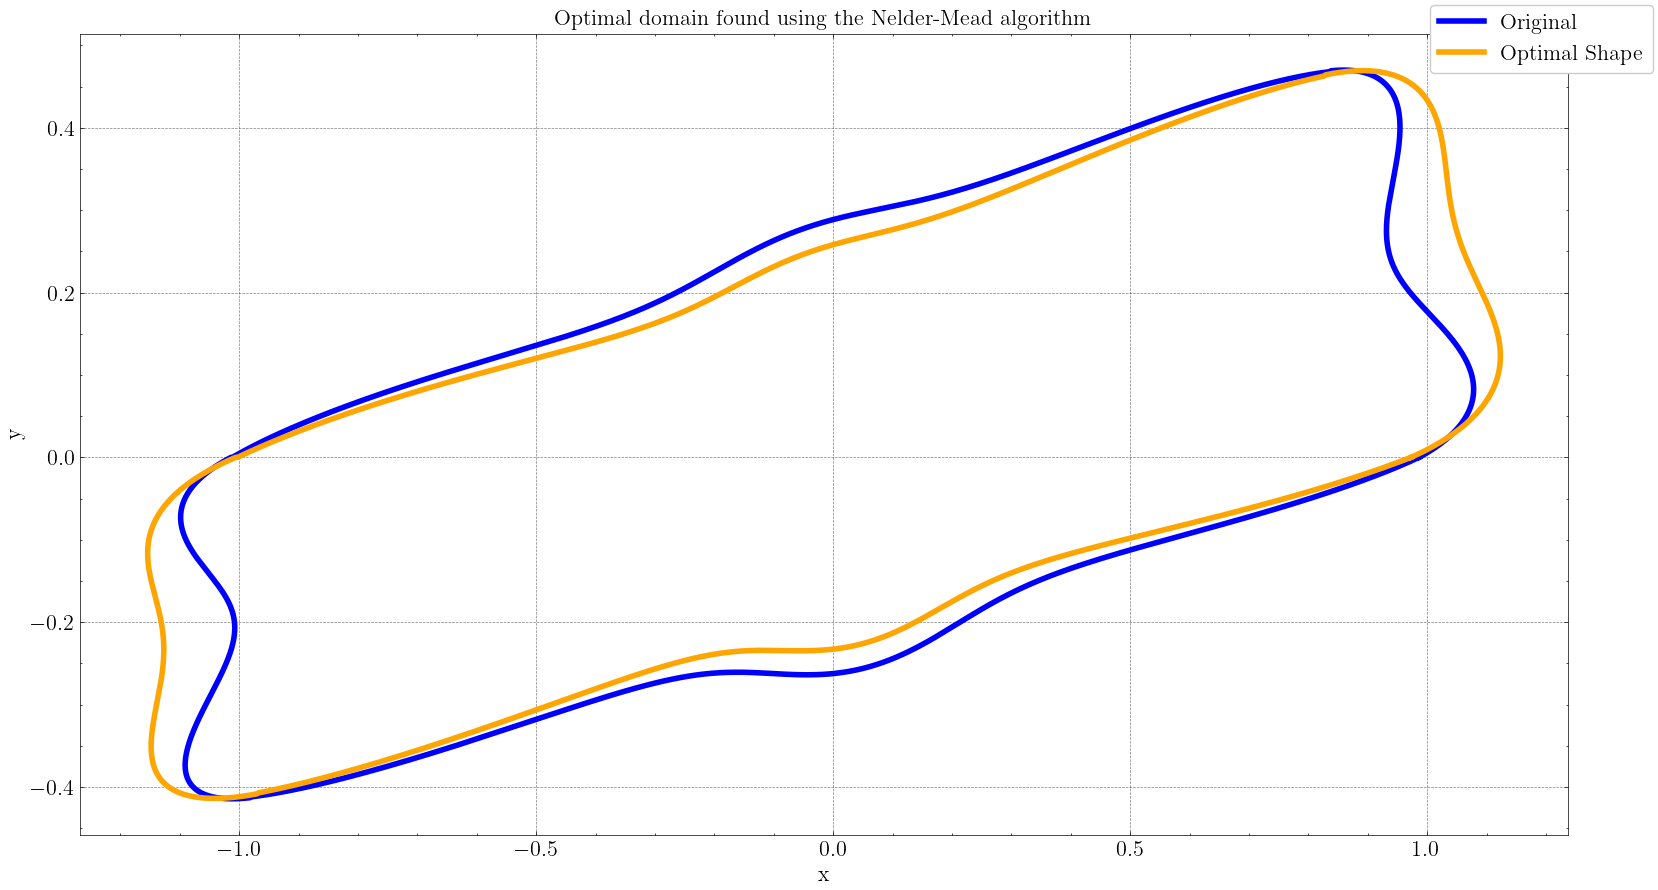
\includegraphics[width=0.75\linewidth]{Images/Dirac/smooth/nelder_mead_optimal.png}
%     \captionof{figure}{Some smooth domain generated by B-splines.}
%     \label{dirac_nelder_mead_domain}
% \end{figure}

% \begin{figure}[!htb]
%     \centering
%     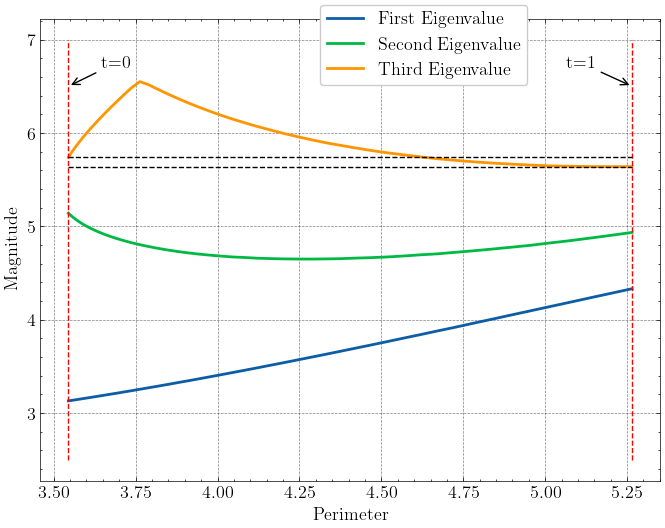
\includegraphics[width=0.75\linewidth]{Images/Dirac/smooth/dirac_val_third.png}
%     \captionof{figure}{Some smooth domain generated by B-splines.}
%     \label{dirac_val_third}
% \end{figure}

\section{Transmission problem simulations}\label{numerical_transmission_simulations}

For the Transmission problem, we now consider the set of equations studied previously in the subchapter \ref{domain_decomp_problem}, given by

\begin{align}\label{transmission_num}
    \begin{cases}
    - \nabla k_i \nabla u_i = f_i, & \text{in }\Omega_i\\
    u_1 - u_2 = 0, & \text{on }\gamma\\
    k_1 \frac{\partial u_1}{\partial n_1} + k_2 \frac{\partial u_2}{\partial n_2} = 0, & \text{on }\gamma\\
    u_i = 0, & \text{on }\Gamma_i.
    \end{cases}
\end{align}

Like before, the domain \(\Omega \subset \mathbb{R}^2\) is divided into two non-overlapping regions \(\Omega_1\) and \(\Omega_2\) such that \(\overline{\Omega} = \overline{\Omega_1} \cup \overline{\Omega_2}\). Their common boundary is denoted by \(\gamma = \partial\Omega_1 \cap \partial\Omega_2\) and the boundary of each domain (minus the common boundary) is also denoted by \(\Gamma_i = \partial\Omega_1\setminus{\gamma}\). In what follows, the source functions \(f_i\) of each domain are constant\footnote{In this work we only considered \(f_i=1\). In any case, we are still working with a general discontinuous source function (if \(k_1 \neq k_2\)). Working with different \textit{continuous} source functions should make no difference in the result. We will also present how to deal with general and continuous source functions.}, and we took \(f_i = 1\). Recall that \(k_1 \geq k_2 > 0\) are constants and \(n_i\) is the (normalized) outward normal to each domain subdomain \(\Omega_i, i=1, 2\), where we shall write \(n=n_1=-n_2\) when we are restricted to the interface.

The procedure presented here is based on \cite{alves2005new} and \cite{alves2021domain}. Given that \(f_i = 1\) for each \(i=1, 2\), a solution of \eqref{transmission_num} can be found by taking the following steps:
\begin{enumerate}
    \item Find a solution for the non-homogeneous problem
    \[
        \begin{cases}
            -\Delta u_1^{NH} = \frac{1}{k_1}\\
            -\Delta u_2^{NH} = \frac{1}{k_2}.
        \end{cases}
    \]
    This can easily be done, and we have
    \[
        \begin{cases}
            u_1^{NH} = -\frac{x_1^2 + x_2^2}{4k_1}\\
            u_2^{NH} = -\frac{x_1^2 + x_2^2}{4k_2};
        \end{cases}
    \]
    \item Then we solve the homogeneous problem
    \begin{align}\label{transmission_num_homo}
        \begin{split}
        - \Delta u_i^H &= 0, \; \text{in }\Omega_i\\
        u_1^H - u_2^H &= u_2^{NH}- u_1^{NH}, \; \text{on }\gamma\\
        k_1 \frac{\partial u_1}{\partial n_1} - k_2 \frac{\partial u_2}{\partial n_1} &= k_2 \frac{\partial u_2^{NH}}{\partial n_1}  - k_1 \frac{\partial u_1^{NH}}{\partial n_1}, \; \text{on }\gamma\\
        u_i &= - u_i^{NH}, \; \text{on }\Gamma_i;
        \end{split}
    \end{align}
    \item Finally, the solution of \eqref{transmission_num} is \(u_i = u_i^H + u_i^{NH}\).
\end{enumerate}
For general source functions, the steps above can also be used: however, it may not be possible to find a closed solution in the first step. In this case, \textbf{1.} must be solved numerically. A popular choice is to use \acp{RBF} (see \cite{golberg1996improved} for example), like the thin plate spline
\[
    \varphi(r) = r^2 \log r,     
\]
and find the coefficients \(\alpha_j\) in \(f_i(x_k) = \tilde{f}_i(x_k) = \sum_{j=1}^{n} \alpha_j \varphi_j(x_k)\) using least square methods, where \(x_k\) are collocation points. Finally, one can analytically solve the equation \(-\Delta \Psi_j = \varphi_j\) to recover the non-homogeneous solutions \(u_1^{NH}\) and \(u_2^{NH}\). In \cite{alves2005new} and \cite{alves2021domain} a different approach was suggested using the fundamental solutions of the Helmholtz equation instead of the classical \acp{RBF}; that method is known today as \textit{Kansa-MFS method}.

In what follows, the numerical results illustrate the accuracy of the method in simply connected 2D domains. Let \(N_i\) denote the number of source points for each domain \(i\), such that \(N=N_1+N_2\). We denote the approximate solution by
\[
    \tilde{u} = \begin{cases}
        \tilde{u}_1, & \text{in } \Omega_1\\
        \tilde{u}_2, & \text{in } \Omega_2,
    \end{cases}
\]
where
\begin{align*}
    &\tilde{u}_1(x) = \sum_{j=1}^{N_1} \alpha^{(1)}_j \Phi\left(x-y_j^{(1)}\right)\\
    &\tilde{u}_2(x) = \sum_{j=1}^{N_2} \alpha^{(2)}_j \Phi\left(x-y_j^{(1)}\right).
\end{align*}
Let \(M_i\) be the number of boundary collocation points \(x^{(i)}_{m}\) for each \(\Omega_i\) and \(M=M_1+M_2\). We also consider \(Q\) interface points \(z_q \in \gamma\) with \(q=1,\dots,Q\). Then, a full block system is written as
\begin{equation}\label{MFS_transmission_classical_matrices_system}
    \renewcommand{\arraystretch}{1.75} % Increase spacing between rows of the matrices
    \begin{bmatrix}
        \left[\Phi\left(x^{(1)}_{m}-y_j^{(1)}\right)\right] & [0] \\
        [0] & \left[\Phi\left(x^{(2)}_{m}-y_j^{(2)}\right)\right] \\
        \left[\Phi\left(z_q-y_j^{(1)}\right)\right] & \left[-\Phi\left(z_q-y_j^{(2)}\right)\right] \\
        \left[k_1\partial_n \Phi\left(z_q-y_j^{(1)}\right)\right] & \left[-k_2 \partial_n \Phi\left(z_q-y_j^{(2)}\right)\right]
    \end{bmatrix}
    \begin{bmatrix}
        \left[\alpha^{(1)}_j\right]\\
        \left[\alpha^{(2)}_j\right]
    \end{bmatrix}=
    \begin{bmatrix}
        \left[-u_1^{NH}(x^{(1)}_{m})\right]\\
        \left[-u_2^{NH}(x^{(2)}_{m})\right]\\
        \left[u_2^{NH}(z_q)-u_1^{NH}(z_q)\right]\\
        \left[k_2 \partial_n u_2^{NH}(z_q)- k_1 \partial_n u_1^{NH}(z_q)\right]\\
    \end{bmatrix}
\end{equation}

Most of the examples below do not have an analytical solution: only in the subchapter \ref{transmission_val_subsection}, when we test the results against a known solution, we can find the absolute error. In the other cases, we are only interested in the relative error, i.e, the boundary error (against which we can compare since \(u_i=0\) in \(\Gamma_i\)) and the interface error by checking the transmission conditions on \(\gamma\):
\begin{itemize}
    \item \(\norm*{\tilde{u}_i - 0}_{L^2(\Gamma_i)}\), \(i=1, 2\): boundary collocation error;
    \item \(\norm*{\tilde{u}_1 - \tilde{u}_2}_{L^2(\gamma)}\), \(i=1, 2\): continuity error (\(C^0\)) of \(\tilde{u}\) across \(\gamma\);
    \item \(\norm*{k_1 \partial_n\tilde{u}_1 - k_2 \partial_n\tilde{u}_2}_{L^2(\gamma)}\), \(i=1, 2\): continuity error \(C^1\) of \(\partial_n\tilde{u}\) across \(\gamma\).
\end{itemize}
From a numerical point of view, let \(\mathcal{I}\) be the sample of test points. The \(L^2\) norm is discretized into the Root Mean Squared Error (\ac{RMSE}) which is equivalent to the \(l^2\) norm and is given by
\[
    \norm*{u-\tilde{u}}= \sqrt{\frac{1}{\#\mathcal{I}} \sum_{z \in \mathcal{I}} \abs{u(z)-\tilde{u}(z)}^2}.
\]
For every result below the number of sample test points is 5 times larger than the sample used to find the coefficients of the \ac{MFS}, and we fix \(k_2=1\) since the ratio \(\frac{k_1}{k_2}\) is responsible for the behavior of the solutions near the interface. 

\subsection{Numerical validation of the method}\label{transmission_val_subsection}

First, we start by testing the numerical algorithm for the unit disk \(\mathbb{D}\), with \(k_1=k_2=1\). From Theorem \ref{equivalence_transmission}, we know that the system of differential equations \eqref{transmission_num} is equivalent to the Poisson equation
\begin{align}\label{transmission_disk}
    \begin{split}
        -\Delta u = 1, & \text{ in } \mathbb{D}\\
        u = 0, & \text{ on } \partial\mathbb{D},
    \end{split}
\end{align}
and is easy to see that the exact solution of Equation \eqref{transmission_disk} is given in polar coordinates by \(u(r, \theta) = \frac{1-r^2}{4}\). 

\begin{figure}[!htb]
    \centering
    \begin{minipage}{.5\textwidth}
      \centering
      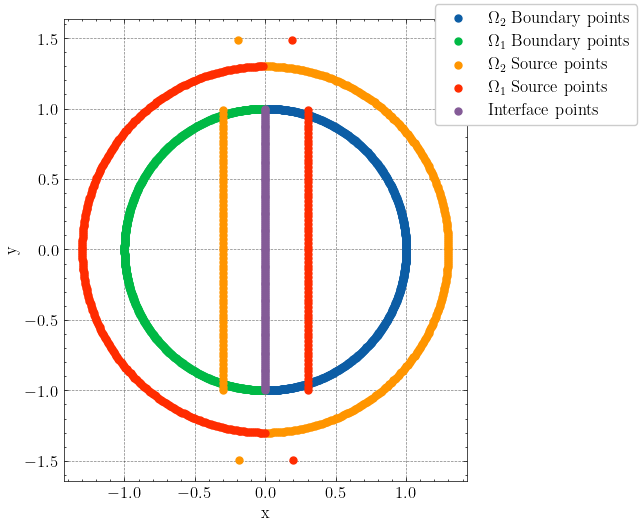
\includegraphics[width=1\linewidth]{Images/Transmission/Circle_val_col_points_600_150.png}
      \captionsetup{width=0.9\linewidth} % Adjust the width of the caption
      \captionof{figure}{Configuration of the boundary, source, and interface points. Each domain has 600 boundary points, 377 source points and the common interface has 100 points.}
      \label{transmission_disk_col}
    \end{minipage}%
    %\hspace{0.5cm} % Add some horizontal space between the figures
    \begin{minipage}{.5\textwidth}
      \centering
      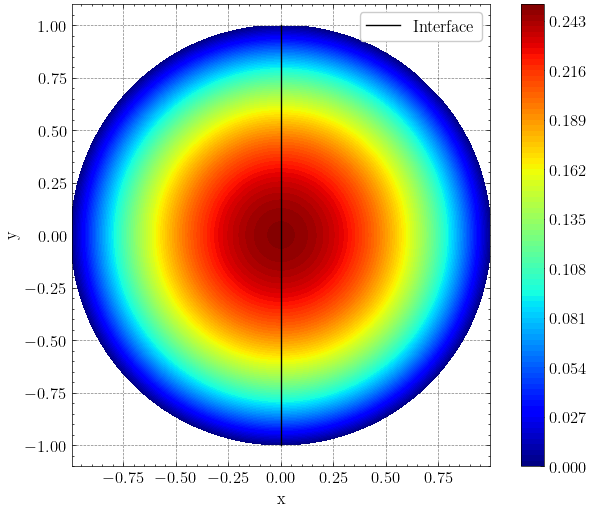
\includegraphics[width=1\linewidth]{Images/Transmission/Circle_val_contour_600_150.png}
      \captionsetup{width=0.9\linewidth} % Adjust the width of the caption
      \captionof{figure}{Numerical approximation of the \ac{BVP} \eqref{transmission_disk} under the conditions presented in Figure \ref{transmission_disk_col}}
      \label{transmission_disk_plot}
    \end{minipage}
\end{figure}

The absolute error between the approximate solution and the exact solution can then be calculated for each domain point. The sample points to compute the absolute error were generated in a uniform grid and were also used to plot Figure \ref{transmission_disk_plot}. The method described at the end of the subchapter \ref{density_proofs_section} was used to place the source points, where \(\eta=0.3\).

\begin{table}[htbp]
    \centering
    \begin{tabular}{cccccc}
        \toprule
        \multirow{2}{*}{\textbf{Boundary/Interface Points}} & \multicolumn{2}{c}{\textbf{Boundary Error}} & \multicolumn{2}{c}{\textbf{Absolute Error}} \\
        \cmidrule(lr){2-3} \cmidrule(lr){4-5}
        & \textbf{Domain 1} & \textbf{Domain 2} & \textbf{Domain 1} & \textbf{Domain 2} \\
        \midrule
        600/150 & $9.759\times10^{-12}$ & $9.541\times10^{-12}$ & $1.465\times10^{-11}$ & $1.439\times10^{-11}$ \\
        500/100 & $3.667\times10^{-11}$ & $3.945\times10^{-11}$ & $9.382\times10^{-11}$ & $9.310\times10^{-11}$ \\
        412/100 & $3.721\times10^{-11}$ & $5.036\times10^{-11}$ & $9.652\times10^{-11}$ & $9.584\times10^{-11}$ \\
        \bottomrule
    \end{tabular}
    \caption{Numerical errors for the boundary and the whole Domains \(\Omega_1\) and \(\Omega_2\)}
    \label{tab:transmission_results_1}
\end{table}


\begin{table}[htbp]
    \centering
    \begin{tabular}{cccc}
      \toprule
      \textbf{Boundary/Interface Points} & \textbf{Interface \(C^0\) Error} & \textbf{Interface \(C^1\) Error} & \textbf{Condition number} \\
      \midrule
      600/150 & $6.945\times10^{-11}$ & $1.841\times10^{-11}$ & $2.528\times 10^{19}$\\
      500/100 & $3.910\times10^{-10}$ & $1.100\times10^{-10}$ & $2.382\times 10^{18}$\\
      412/100 & $4.035\times10^{-10}$ & $1.342\times10^{-10}$ & $7.597\times 10^{17}$\\
      \bottomrule
    \end{tabular}
    \caption{Numerical error on the interface \(\gamma\). The condition number of the matrix is also presented.}
    \label{tab:transmission_results_2}
\end{table}

The numerical results presented in Tables \ref{tab:transmission_results_1} and \ref{tab:transmission_results_2} are not yet optimal. When considering a larger value of \(\eta\), the results increase by more than two orders of magnitude, but this also leads to a significant increase in the already very high condition number (see Table \ref{tab:transmission_results_2}), as expected. Despite this, the results show great promise, which was anticipated due to the domain's analyticity.

As mentioned previously, the Method of Fundamental Solutions (\ac{MFS}) yields better results in highly regular domains, even when considering curved geometries. However, increasing the number of boundary and interface collocation points improves the accuracy of the solution. It is important to note that a larger number of points also escalates the condition number, making the problem more challenging to solve accurately.

The inclusion of the "corner" source points, as depicted in Figure \ref{transmission_disk_col}, also significantly impacts the method's accuracy. These source points, strategically added to capture the behavior near the interface corner, can be inside one of the domains as the solution will be split into two parts.

\subsection{Results for the rectangle}

In this subchapter a rectangular domain \([-1, -0.5] \times [1, 0.5]\) with a vertical interface along the line \(x=0\) is considered. We are now interested to study the problem for \(k_1 \neq k_2\) where \(k_2=1\) is fixed. The results below were conducted with 600 boundary points and 404 source points for each domain. The number of interface points is 150 and \(\eta=0.08\).

\begin{figure}[!htb]
    \centering
    \begin{minipage}{.5\textwidth}
      \centering
      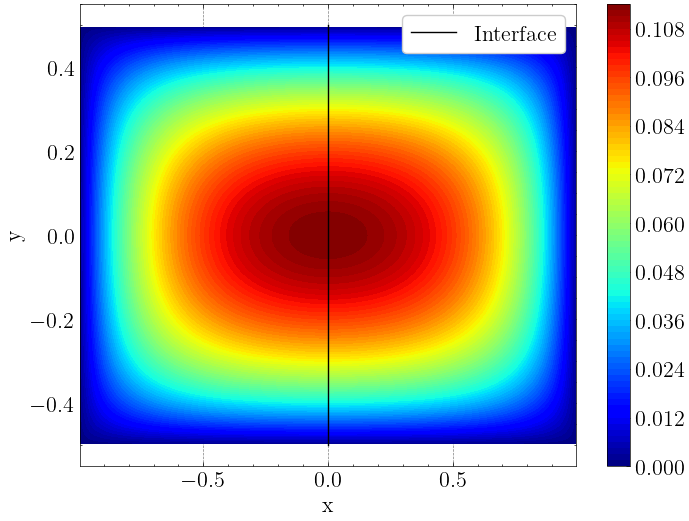
\includegraphics[width=\linewidth]{Images/Transmission/Rectangle_contour_600_150_k1_1.png}
      \caption{Numerical simulation with  \(k_1=1\).}
      \label{transmission_rectangle_plot_k1_1}
    \end{minipage}%
    \begin{minipage}{.5\textwidth}
      \centering
      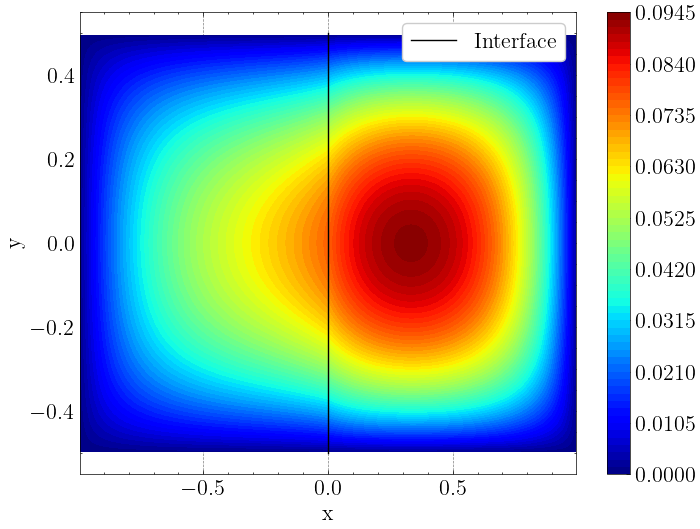
\includegraphics[width=\linewidth]{Images/Transmission/Rectangle_contour_600_150_k1_2.png}
      \caption{Numerical simulation with \(k_1=2\).}
      \label{transmission_rectangle_plot_k1_2}
    \end{minipage}
    
    \vspace{0.5cm} % Add some vertical space between the rows of figures
    
    \begin{minipage}{.6\textwidth}
      \centering
      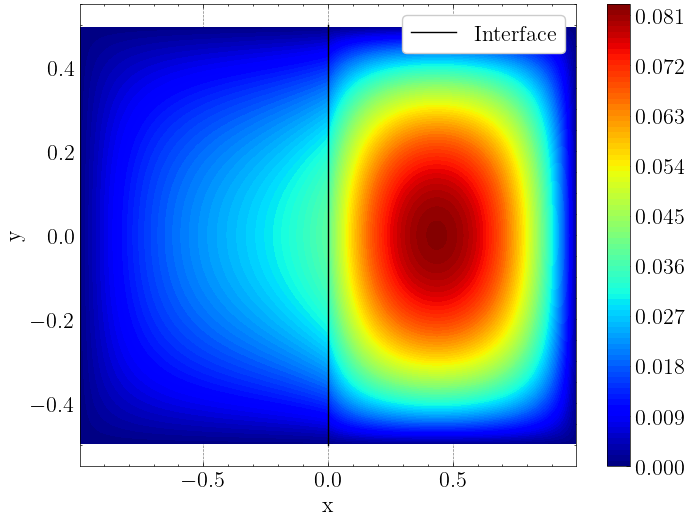
\includegraphics[width=0.9\linewidth]{Images/Transmission/Rectangle_contour_600_150_k1_5.png}
      \caption{Numerical simulation with  \(k_1=5\).}
      \label{transmission_rectangle_plot_k1_5}
    \end{minipage}
    
    \caption*{Numerical approximations of the \ac{BVP} for a rectangular domain with different \(k_1\) values.}
    \label{transmission_rectangle_plots}
\end{figure}

\begin{table}[htbp]
    \centering
    \begin{tabular}{cccccc}
      \toprule
      \multirow{2}{*}{\textbf{\(k_1\) value}} & \multicolumn{2}{c}{\textbf{Boundary Error}} & \multicolumn{2}{c}{\textbf{Interface Errors}} & \multirow{2}{*}{\textbf{Condition number}} \\
      \cmidrule(lr){2-3} \cmidrule(lr){4-5}
      & \textbf{Domain 1} & \textbf{Domain 2} & \textbf{\(C^0\)} & \textbf{\(C^1\)} & \\
      \midrule
      1 & $7.775\times10^{-8}$ & $7.779\times10^{-8}$ & $4.732\times10^{-9}$ & $7.589\times10^{-9}$ & $2.331\times 10^{13}$\\
      2 & $4.398\times10^{-8}$ & $8.614\times10^{-8}$ & $2.499\times10^{-6}$ & $7.868\times10^{-8}$ & $3.623\times 10^{13}$\\
      3 & $2.181\times10^{-8}$ & $1.036\times10^{-7}$ & $3.838\times10^{-6}$ & $1.551\times10^{-7}$ & $8.182\times 10^{13}$\\
      \bottomrule
    \end{tabular}
    \caption{Numerical relative error on the boundary and in the interface \(\gamma\)}
    \label{tab:transmission_results_rectangle}
\end{table}

In Figures \ref{transmission_rectangle_plot_k1_1}, \ref{transmission_rectangle_plot_k1_2}, and \ref{transmission_rectangle_plot_k1_5}, we present the numerical approximation for different \(k_1\) values. Observe that increasing \(k_1\) breaks the symmetry of the solution, which shifts from \(\Omega_1\) (the domain on the left) to \(\Omega_2\) (the domain on the right). Table \ref{tab:transmission_results_rectangle} summarizes the results for different \(k_1\) values. While the results are slightly worse than the previous ones due to the worse domain regularity, they still preserve high accuracy. It is worth noting that for different values of \(k_1\) and \(k_2\), the accuracy of the method decreases. This is also to be expected, as we are dealing with a discontinuous source function, which decreases the regularity of the solution.

Notice that the condition number for the rectangle is smaller than the one presented in Table \ref{tab:transmission_results_2} for the unit disk. This is a consequence of a smaller value of \(\eta\), which in this case appears to be optimal since increasing its value decreases the overall accuracy.

\subsection{Results for an L-shape domain with enrichment}

In the previous subchapter, a domain with corners was analyzed. However, it still preserved some regularity, and the \ac{MFS} with classical basis functions was able to capture its corner's behavior, as explained in Remark \ref{particular_solutions}. In what follows, we are going to study the case of an L-shape, a non-convex domain with singular corners. Two different interfaces will be considered: first, the usual interface along the line \(x=0\); then, along its symmetry axis with the line \(y=\frac{1}{2}x\).

Consider the L-shape given in Figure \ref{transmission_L_shape_config}. The left and right subdomains are denoted by \(\Omega_1\) and \(\Omega_2\), respectively. The number of interface points is 300, and the number of source points for each domain is 428. The number of boundary collocation points for \(\Omega_1\) and \(\Omega_2\) is 710 and 639, respectively.

\begin{figure}[!htb]
    \centering
    \begin{minipage}{.5\textwidth}
        \centering
        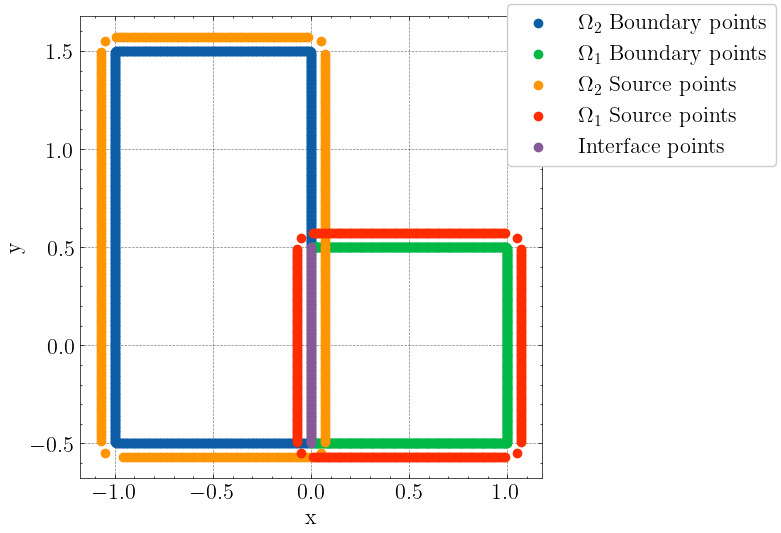
\includegraphics[width=0.8\linewidth]{Images/Transmission/L_shape_2_rectangles_col_points.png}
        \captionsetup{width=0.9\linewidth} % Adjust the width of the caption
        \caption{L-shape domain with a vertical interface. Configuration of the boundary, source, and interface points.}
        \label{transmission_L_shape_config}
    \end{minipage}%
    %\hspace{0.2cm} % Add some horizontal space between the figures
    \begin{minipage}{.5\textwidth}
        \centering
        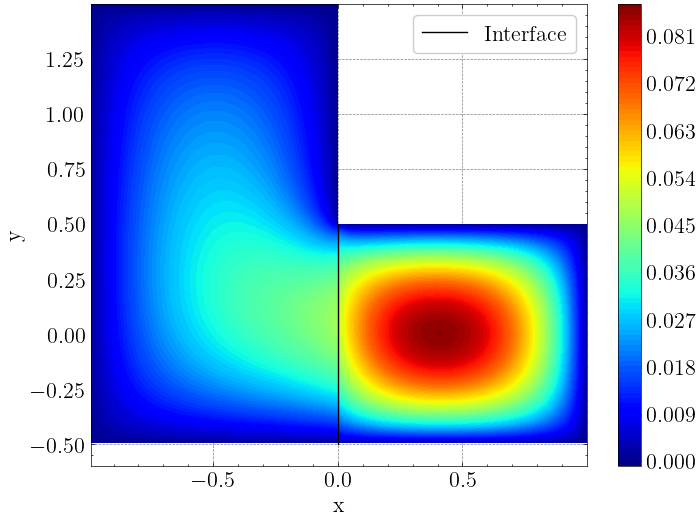
\includegraphics[width=\linewidth]{Images/Transmission/L_shape_2_rectangles_k1_5.png}
        \captionsetup{width=0.9\linewidth} % Adjust the width of the caption
        \caption{Numerical approximation of the \ac{BVP} for an L-shape domain with interface along \(x=0\) and \(k_1=5\).}
        \label{transmission_L_shape_k1_5}
    \end{minipage}
\end{figure}

In Table \ref{tab:transmission_results_L_shape_rectangles}, the results without resorting to enrichment are presented. It is evident that the method yields poorer results due to the lower regularity of the domain. Particularly, the interface error (mainly the \(C^0\) error) is significantly higher compared to previous cases, even when considering more collocation points on the interface. It appears that the domain itself poses more challenges than the discontinuous source function when considering different values for \(k_1\) and \(k_2\). In Figure \ref{transmission_L_shape_k1_5}, it is even possible to see that there already exists some small jump near the edges of the interface.

\begin{table}[!htbp]
    \centering
    \begin{tabular}{cccccc}
      \toprule
      \multirow{2}{*}{\textbf{\(k_1\) value}} & \multicolumn{2}{c}{\textbf{Boundary Error}} & \multicolumn{2}{c}{\textbf{Interface Errors}} & \multirow{2}{*}{\textbf{Condition number}} \\
      \cmidrule(lr){2-3} \cmidrule(lr){4-5}
      & \textbf{Domain 1} & \textbf{Domain 2} & \textbf{\(C^0\)} & \textbf{\(C^1\)} & \\
      \midrule
      1 & $7.853\times10^{-5}$ & $1.155\times10^{-4}$ & $2.916\times10^{-3}$ & $2.155\times10^{-5}$ & $5.587\times 10^{12}$ \\
      2 & $8.152\times10^{-5}$ & $1.350\times10^{-4}$ & $3.835\times10^{-3}$ & $1.149\times10^{-5}$ & $8.161\times 10^{12}$ \\
      5 & $7.079\times10^{-5}$ & $1.378\times10^{-4}$ & $4.085\times10^{-3}$ & $5.411\times10^{-5}$ & $1.776\times 10^{13}$ \\
      \bottomrule
    \end{tabular}
    \caption{Numerical relative error on the boundary and in the interface \(\gamma\)}
    \label{tab:transmission_results_L_shape_rectangles}
\end{table}


One of the major problems for the method is the behavior of the solution near the degenerate corner with \(\pi\) radians in \(\Omega_1\), where some singularity may exist due to the different boundary conditions imposed there. Notice that for \(\Omega_2\) there exists no problem since the interface edges make a right angle with the adjacent edges. Therefore, we consider some particular solutions which describe the solution in the domain \(\Omega_1\). In this case, we are going to use Dirichlet-Neummann particular solutions, like the ones presented in \ref{m_particular_solutions}, centered in the singular corner. Let
\begin{equation}\label{pat_sol_L_shape_rect}
    v_{p_1}(r, \theta) = \alpha_{p_1} r^{\alpha_{p_1}} \sin(\alpha_{p_1}(\theta - \theta_1))
\end{equation}
where
\[
    \alpha_{p_1} = \frac{(p+\frac{1}{2})\pi}{\Theta},
\]
\(\theta_1 = \frac{\pi}{2}\) is the angle shift, \(\Theta = \pi\) is the total angle amplitude,  and the coordinates \(r\) and \(\theta\) are given in polar coordinates by
\[
    r(x,y) = \sqrt{x^2+y^2} \quad \theta(x,y)=\begin{cases}
        \arctan(\frac{y}{x}),& \text{if} \arctan(\frac{y}{x})>0\\
        \arctan(\frac{y}{x})+2\pi,& \text{if} \arctan(\frac{y}{x})\leq0.
    \end{cases}
\]
By differentiating Equation \eqref{pat_sol_L_shape_rect} in cartesian coordinates and substituting polar coordinates again we find that
\begin{equation*}
    \nabla v_{p_1}(r, \theta) = \left(-\frac{(2 \pi  {p_1}+\pi )^2 r^{\frac{2 \pi  {p_1}+\pi }{2 \Theta }} \sin \left(\theta +\frac{\pi  \left(p_1+\frac{1}{2}\right) (s-\theta )}{\Theta }\right)}{4 \Theta ^2 r},\frac{(2 \pi  p_1+\pi )^2 r^{\frac{2 \pi  p_1+\pi }{2 \Theta }} \cos \left(\theta +\frac{\pi  \left(p_1+\frac{1}{2}\right) (s-\theta )}{\Theta }\right)}{4 \Theta ^2 r}\right).
\end{equation*}
Finally, considering the truncated expansion
\begin{equation}\label{num_particular_L_shape_rect_equation}
    \phi(r,\theta)=\sum_{p_1=0}^{P_1} \beta_{p_1} v_{p_1}(r, \theta),
\end{equation}
and expanding the matrix in \eqref{MFS_transmission_classical_matrices_system}, one can write
\begin{equation}\label{transmission_mat_L_rect_exp}
    \renewcommand{\arraystretch}{1.75} % Increase spacing between rows of the matrices
    \begin{bmatrix}
        \left[\Phi\left(x^{(1)}_{m}-y_j^{(1)}\right)\right] & [0] & \left[\phi(r\left(x_m\right),\theta\left(x_m\right))\right]\\
        [0] & \left[\Phi\left(x^{(2)}_{m}-y_j^{(2)}\right)\right] & \left[0\right]\\
        \left[\Phi\left(z_q-y_j^{(1)}\right)\right] & \left[-\Phi\left(z_q-y_j^{(2)}\right)\right] & \left[\phi(r\left(z_k\right),\theta\left(z_q\right))\right]\\
        \left[k_1\partial_n \Phi\left(z_q-y_j^{(1)}\right)\right] & \left[-k_2 \partial_n \Phi\left(z_q-y_j^{(2)}\right)\right] & \left[k_1 \partial_n\phi(r\left(z_q\right),\theta\left(z_q\right))\right]
    \end{bmatrix}
\end{equation}

Table \ref{tab:transmission_results_L_shape_rectangles_particular} presents the results after applying the enrichment technique for the previous \(k_1\) values. In the expansion \eqref{num_particular_L_shape_rect_equation}, different values for \(P_1\) were considered. For example, for the first section of the Table, we set \(P_1=1\). After some simulations, it became clear that increasing \(P_1\) would not give better results. Furthermore, since the form of Equation \eqref{num_particular_L_shape_rect_equation} is also valid for the exterior problem, negative values of \(p_1\) were considered. Interestingly, when adding solutions for the exterior problem, better results were achieved. Not only did the error decrease for the boundary \(\Gamma_i\) of each domain, but better results were also achieved on the interface.

\begin{table}[!htbp]
    \centering
    \begin{longtable}{ccccccc}
        \toprule
        \multicolumn{1}{c}{\textbf{\(p_1\) values}} & \multicolumn{1}{c}{\textbf{\(k_1\) value}} & \multicolumn{2}{c}{\textbf{Boundary Error}} & \multicolumn{2}{c}{\textbf{Interface Errors}} & \multicolumn{1}{c}{\textbf{Condition number}} \\
        \cmidrule(lr){2-2} \cmidrule(lr){3-4} \cmidrule(lr){5-6} \cmidrule(lr){7-7}
        & & \textbf{Domain 1} & \textbf{Domain 2} & \textbf{\(C^0\)} & \textbf{\(C^1\)} & \\
        \midrule
        \endfirsthead % Header for the first page
        \multicolumn{7}{l}{{\footnotesize\emph{Continued from previous page}}} \\
        \toprule
        \multicolumn{1}{c}{\textbf{\(p\) value}} & \multicolumn{1}{c}{\textbf{\(k_1\) value}} & \multicolumn{2}{c}{\textbf{Boundary Error}} & \multicolumn{2}{c}{\textbf{Interface Errors}} & \multicolumn{1}{c}{\textbf{Condition number}} \\
        \cmidrule(lr){2-2} \cmidrule(lr){3-4} \cmidrule(lr){5-6} \cmidrule(lr){7-7}
        & & \textbf{Domain 1} & \textbf{Domain 2} & \textbf{\(C^0\)} & \textbf{\(C^1\)} & \\
        \midrule
        \endhead % Header for subsequent pages
        \midrule[\heavyrulewidth] % Horizontal line
        \multicolumn{7}{r}{{\footnotesize\emph{Continued on next page}}} \\
        \endfoot % Footer for subsequent pages
        \bottomrule
        \endlastfoot % Footer for the last page
        
        % Data for p = [0, 1]
        0, 1 & 1 & $2.965\times10^{-5}$ & $7.907\times10^{-5}$ & $2.94\times10^{-3}$ & $2.624\times10^{-5}$ & $5.584\times10^{12}$ \\
        & 2 & $2.203\times10^{-5}$ & $6.657\times10^{-5}$ & $1.86\times10^{-3}$ & $2.068\times10^{-5}$ & $8.156\times10^{12}$ \\
        & 5 & $2.203\times10^{-5}$ & $6.657\times10^{-5}$ & $1.86\times10^{-3}$ & $2.068\times10^{-5}$ & $8.156\times10^{12}$ \\
        \midrule[\heavyrulewidth] % Horizontal line
        
        % Data for p = [-1, 0, 1]
        -1, 0, 1 & 1 & $8.627\times10^{-6}$ & $4.132\times10^{-5}$ & $7.68\times10^{-4}$ & $6.876\times10^{-6}$ & $5.585\times10^{12}$ \\
        & 2 & $7.333\times10^{-6}$ & $2.791\times10^{-5}$ & $6.01\times10^{-4}$ & $2.555\times10^{-5}$ & $8.157\times10^{12}$ \\
        & 5 & $4.271\times10^{-6}$ & $1.118\times10^{-5}$ & $2.69\times10^{-4}$ & $4.166\times10^{-5}$ & $1.775\times10^{13}$ \\
        \midrule[\heavyrulewidth] % Horizontal line

        % Data for p = [-2, -1, 0, 1]
        -2, -1, 0, 1 & 1 & $3.898\times10^{-6}$ & $5.975\times10^{-6}$ & $1.44\times10^{-3}$ & $2.505\times10^{-6}$ & $4.156\times10^{14}$ \\
        & 2 & $2.584\times10^{-6}$ & $2.514\times10^{-6}$ & $9.69\times10^{-4}$ & $1.048\times10^{-5}$ & $4.156\times10^{14}$ \\
        & 5 & $1.119\times10^{-6}$ & $6.838\times10^{-7}$ & $4.89\times10^{-4}$ & $1.106\times10^{-5}$ & $4.156\times10^{14}$ \\
        \midrule[\heavyrulewidth] % Horizontal line
    \end{longtable}
    \caption{Numerical relative error on the boundary and in the interface \(\gamma\) after considering particular (angular) solutions}
    \label{tab:transmission_results_L_shape_rectangles_particular}
\end{table}

To finish this subchapter, and as stated in the beginning, we present a more complicated L-shape domain where the interface is drawn along its axis of symmetry. In this case, notice that there are two singular corners, both with \(\frac{3}{4}\pi\) radians\footnote{The other two corners have an angle of \(\frac{\pi}{4}\) radians which cause no problem for the classical \ac{MFS} basis functions.}. In Figure \ref{transmission_L_shape_col_axis_config} the configuration is presented, where the left domain is \(\Omega_1\) and the right domain \(\Omega_2\). The number of interface points and source points for each domain is still 300 and 428, respectively. We also chose 628 boundary collocation points for both domains. Table \ref{tab:transmission_results_L_shape_axis} summarizes the results without considering particular solutions.

\begin{figure}[!htb]
    \centering
    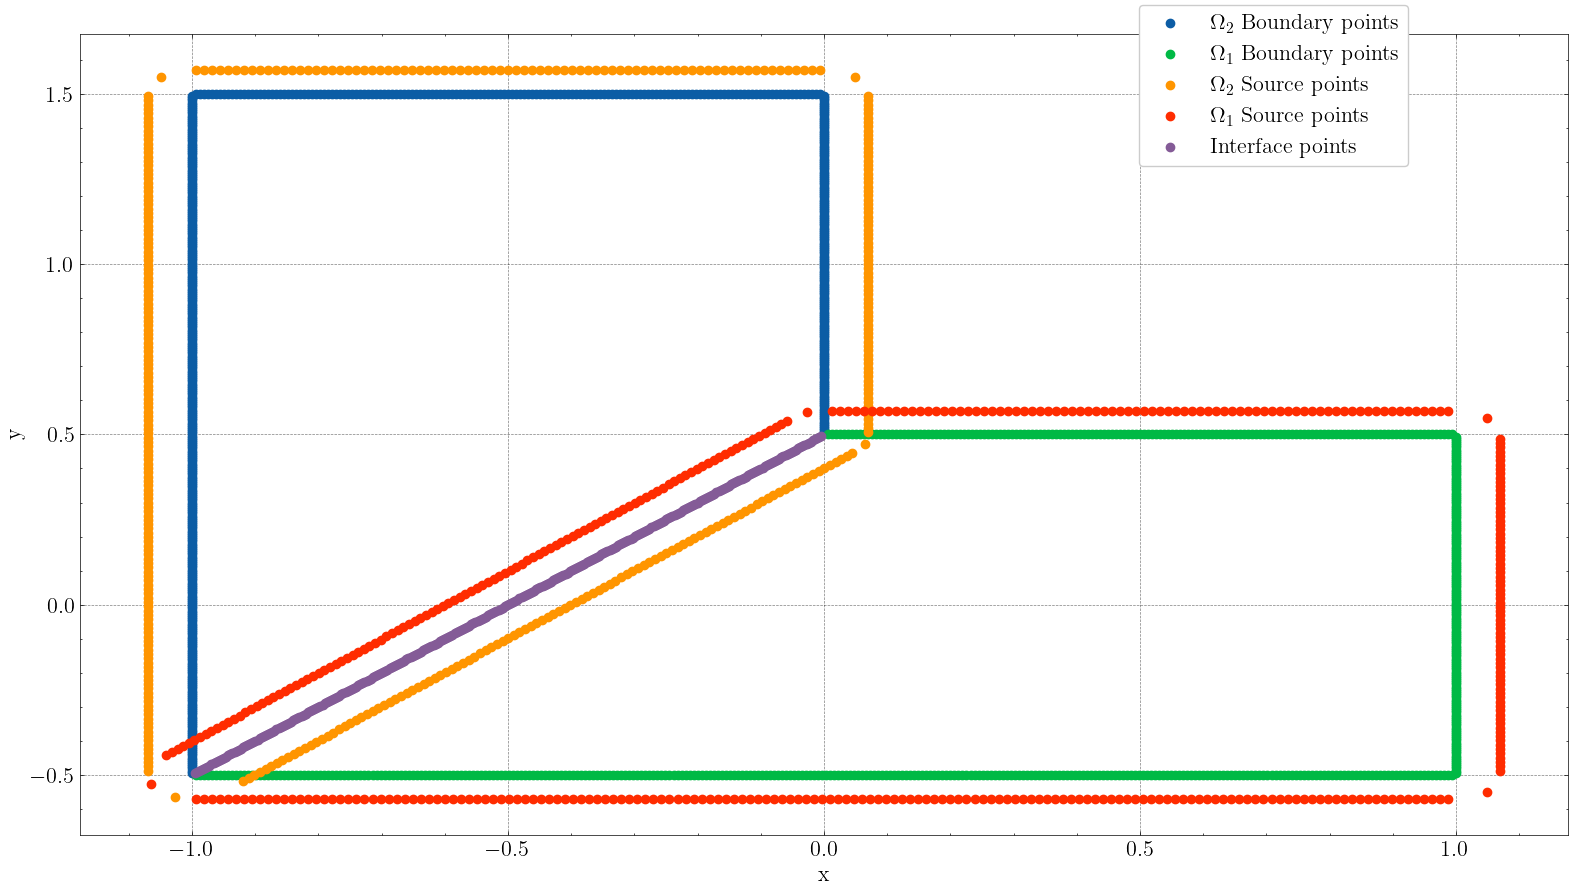
\includegraphics[height=0.4\linewidth,width=0.53\linewidth]{Images/Transmission/L_shape_2_axis_col_points.png}
    %\captionsetup{width=0.9\linewidth} % Adjust the width of the caption
    \caption{L-shape domain with the interface on the symmetry axis. Configuration of the boundary, source, and interface points.}
    \label{transmission_L_shape_col_axis_config}
\end{figure}

\begin{table}[!htbp]
    \centering
    \begin{tabular}{cccccc}
      \toprule
      \multirow{2}{*}{\textbf{\(k_1\) value}} & \multicolumn{2}{c}{\textbf{Boundary Error}} & \multicolumn{2}{c}{\textbf{Interface Errors}} & \multirow{2}{*}{\textbf{Condition number}} \\
      \cmidrule(lr){2-3} \cmidrule(lr){4-5}
      & \textbf{Domain 1} & \textbf{Domain 2} & \textbf{\(C^0\)} & \textbf{\(C^1\)} & \\
      \midrule
      1 & $1.812\times10^{-4}$ & $2.060\times10^{-4}$ & $7.305\times10^{-3}$ & $8.018\times10^{-5}$ & $1.050\times 10^{10}$ \\
      2 & $1.398\times10^{-4}$ & $9.729\times10^{-5}$ & $5.986\times10^{-4}$ & $5.505\times10^{-5}$ & $1.646\times 10^{10}$ \\
      5 & $7.096\times10^{-5}$ & $3.030\times10^{-5}$ & $1.528\times10^{-3}$ & $4.348\times10^{-5}$ & $3.730\times 10^{10}$ \\
      \bottomrule
    \end{tabular}
    \caption{Numerical relative error on the boundary and in the interface \(\gamma\)}
    \label{tab:transmission_results_L_shape_axis}
\end{table}

Since particular solutions will be added to the singular corners in \(\Omega_2\), one should now consider Neummann-Dirichlet particular solutions centered in the singular corner. These particular solutions have the form
\[
    w_{p_2}(r,\theta) = \alpha_{p_2} r^{\alpha_{p_2}}\cos(\alpha_{p_2}(\theta-\theta_2)),
\]
where the \(\alpha_{p_2}\) coefficients are the same as before, \(\Theta = \frac{3}{4}\pi\) and \(\theta_2=\frac{5}{4}\pi\) is the angle shift. Notice that \(\Theta\) is the same in both domains. The (polar) gradient of \(w\) is now
\begin{equation*}
    \nabla w(r,\theta)_{p_2} = \left(\frac{(2 \pi  {p_2}+\pi )^2 r^{\frac{2 \pi  {p_2}+\pi }{2 \Theta }} \cos \left(\theta +\frac{\pi  \left({p_2}+\frac{1}{2}\right) (s-\theta )}{\Theta }\right)}{4 \Theta ^2 r},\frac{(2 \pi  {p_2}+\pi )^2 r^{\frac{2 \pi  {p_2}+\pi }{2 \Theta }} \sin \left(\theta +\frac{\pi  \left({p_2}+\frac{1}{2}\right) (s-\theta )}{\Theta }\right)}{4 \Theta ^2 r}\right).
\end{equation*}

Considering the expansion \eqref{num_particular_L_shape_rect_equation} for the \(w_{p_2}\) particular solutions, one can add more blocks to the matrix \eqref{transmission_mat_L_rect_exp}. Table \ref{tab:transmission_results_L_shape_axis_particular} shows the results when particular solutions are added to both domains. Once again, negative values of \(p_2\) were considered. Without intending to show too much data (because we would have to account for every combination of \(p_1\) and \(p_2\) values), we fix \(p_2=0, 1\). The reason for this choice is that we noticed better results are achieved when increasing the number of particular solutions in the domain where the diffusion coefficient is increasing. In this case, we are only varying the coefficient \(k_1\), and therefore, we can fix the \(p_2\) values.


\begin{table}[htbp]
    \centering
    \begin{longtable}{ccccccc}
        \toprule
        \multicolumn{1}{c}{\textbf{\(p_1\) values}} & \multicolumn{1}{c}{\textbf{\(k_1\) value}} & \multicolumn{2}{c}{\textbf{Boundary Error}} & \multicolumn{2}{c}{\textbf{Interface Errors}} & \multicolumn{1}{c}{\textbf{Condition number}} \\
        \cmidrule(lr){2-2} \cmidrule(lr){3-4} \cmidrule(lr){5-6} \cmidrule(lr){7-7}
        & & \textbf{Domain 1} & \textbf{Domain 2} & \textbf{\(C^0\)} & \textbf{\(C^1\)} & \\
        \midrule
        \endfirsthead % Header for the first page
        \multicolumn{7}{l}{{\footnotesize\emph{Continued from previous page}}} \\
        \toprule
        \multicolumn{1}{c}{\textbf{\(p\) value}} & \multicolumn{1}{c}{\textbf{\(k_1\) value}} & \multicolumn{2}{c}{\textbf{Boundary Error}} & \multicolumn{2}{c}{\textbf{Interface Errors}} & \multicolumn{1}{c}{\textbf{Condition number}} \\
        \cmidrule(lr){2-2} \cmidrule(lr){3-4} \cmidrule(lr){5-6} \cmidrule(lr){7-7}
        & & \textbf{Domain 1} & \textbf{Domain 2} & \textbf{\(C^0\)} & \textbf{\(C^1\)} & \\
        \midrule
        \endhead % Header for subsequent pages
        \midrule[\heavyrulewidth] % Horizontal line
        \multicolumn{7}{r}{{\footnotesize\emph{Continued on next page}}} \\
        \endfoot % Footer for subsequent pages
        \bottomrule
        \endlastfoot % Footer for the last page
        
        % Data for p = [0, 1]
        0, 1 & 1 & $3.107\times10^{-7}$ & $2.100\times10^{-7}$ & $1.158\times10^{-5}$ & $1.019\times10^{-7}$ & $1.054\times10^{10}$ \\
        & 2 & $1.061\times10^{-7}$ & $6.892\times10^{-7}$ & $6.366\times10^{-5}$ & $7.065\times10^{-8}$ & $1.648\times10^{10}$ \\
        & 5 & $1.207\times10^{-7}$ & $1.141\times10^{-6}$ & $9.544\times10^{-5}$ & $9.487\times10^{-8}$ & $3.732\times10^{10}$ \\
        \midrule[\heavyrulewidth] % Horizontal line
        
        % Data for p = [-1, 0, 1]
        -1, 0, 1 & 1 & $3.319\times10^{-7}$ & $2.026\times10^{-7}$ & $1.813\times10^{-5}$ & $1.048\times10^{-7}$ & $1.054\times10^{10}$ \\
        & 2 & $1.676\times10^{-7}$ & $3.166\times10^{-7}$ & $8.375\times10^{-6}$ & $7.951\times10^{-8}$ & $1.647\times10^{10}$ \\
        & 5 & $9.871\times10^{-8}$ & $4.807\times10^{-7}$ & $1.549\times10^{-6}$ & $5.285\times10^{-8}$ & $3.732\times10^{10}$ \\
        \midrule[\heavyrulewidth] % Horizontal line

        % Data for p = [-2, -1, 0, 1]
        -2, -1, 0, 1 & 1 & $3.070\times10^{-7}$ & $2.415\times10^{-7}$ & $1.610\times10^{-5}$ & $9.893\times10^{-8}$ & $5.659\times10^{12}$ \\
        & 2 & $1.762\times10^{-7}$ & $2.670\times10^{-7}$ & $8.385\times10^{-6}$ & $8.480\times10^{-8}$ & $5.656\times10^{12}$ \\
        & 5 & $9.761\times10^{-8}$ & $3.201\times10^{-7}$ & $1.993\times10^{-6}$ & $6.049\times10^{-8}$ & $5.655\times10^{12}$ \\
        \midrule[\heavyrulewidth] % Horizontal line
    \end{longtable}
    \caption{Numerical relative error on the boundary and in the interface \(\gamma\) after considering particular (angular) solutions}
    \label{tab:transmission_results_L_shape_axis_particular}
\end{table}

% \begin{longtable}{ccccccc}
%         \caption{Numerical relative error on the boundary and in the interface \(\gamma\) after considering particular (angular) solutions}
%         \label{tab:transmission_results_L_shape_axis_particular}
%         \toprule
%         \multicolumn{1}{c}{\textbf{\(p_1\) values}} & \multicolumn{1}{c}{\textbf{\(k_1\) value}} & \multicolumn{2}{c}{\textbf{Boundary Error}} & \multicolumn{2}{c}{\textbf{Interface Errors}} & \multicolumn{1}{c}{\textbf{Condition number}} \\
%         \cmidrule(lr){2-2} \cmidrule(lr){3-4} \cmidrule(lr){5-6} \cmidrule(lr){7-7}
%         & & \textbf{Domain 1} & \textbf{Domain 2} & \textbf{\(C^0\)} & \textbf{\(C^1\)} & \\
%         \midrule
%         \endfirsthead % Header for the first page
%         \multicolumn{7}{l}{{\footnotesize\emph{Continued from previous page}}} \\
%         \toprule
%         \multicolumn{1}{c}{\textbf{\(p\) value}} & \multicolumn{1}{c}{\textbf{\(k_1\) value}} & \multicolumn{2}{c}{\textbf{Boundary Error}} & \multicolumn{2}{c}{\textbf{Interface Errors}} & \multicolumn{1}{c}{\textbf{Condition number}} \\
%         \cmidrule(lr){2-2} \cmidrule(lr){3-4} \cmidrule(lr){5-6} \cmidrule(lr){7-7}
%         & & \textbf{Domain 1} & \textbf{Domain 2} & \textbf{\(C^0\)} & \textbf{\(C^1\)} & \\
%         \midrule
%         \endhead % Header for subsequent pages
%         \midrule[\heavyrulewidth] % Horizontal line
%         \multicolumn{7}{r}{{\footnotesize\emph{Continued on next page}}} \\
%         \endfoot % Footer for subsequent pages
%         \bottomrule
%         \endlastfoot % Footer for the last page
        
%         % Data for p = [0, 1]
%         0, 1 & 1 & $3.107\times10^{-7}$ & $2.100\times10^{-7}$ & $1.158\times10^{-5}$ & $1.019\times10^{-7}$ & $1.054\times10^{10}$ \\
%         & 2 & $1.061\times10^{-7}$ & $6.892\times10^{-7}$ & $6.366\times10^{-5}$ & $7.065\times10^{-8}$ & $1.648\times10^{10}$ \\
%         & 5 & $1.207\times10^{-7}$ & $1.141\times10^{-6}$ & $9.544\times10^{-5}$ & $9.487\times10^{-8}$ & $3.732\times10^{10}$ \\
%         \midrule[\heavyrulewidth] % Horizontal line
        
%         % Data for p = [-1, 0, 1]
%         -1, 0, 1 & 1 & $3.319\times10^{-7}$ & $2.026\times10^{-7}$ & $1.813\times10^{-5}$ & $1.048\times10^{-7}$ & $1.054\times10^{10}$ \\
%         & 2 & $1.676\times10^{-7}$ & $3.166\times10^{-7}$ & $8.375\times10^{-6}$ & $7.951\times10^{-8}$ & $1.647\times10^{10}$ \\
%         & 5 & $9.871\times10^{-8}$ & $4.807\times10^{-7}$ & $1.549\times10^{-6}$ & $5.285\times10^{-8}$ & $3.732\times10^{10}$ \\
%         \midrule[\heavyrulewidth] % Horizontal line

%         % Data for p = [-2, -1, 0, 1]
%         -2, -1, 0, 1 & 1 & $3.070\times10^{-7}$ & $2.415\times10^{-7}$ & $1.610\times10^{-5}$ & $9.893\times10^{-8}$ & $5.659\times10^{12}$ \\
%         & 2 & $1.762\times10^{-7}$ & $2.670\times10^{-7}$ & $8.385\times10^{-6}$ & $8.480\times10^{-8}$ & $5.656\times10^{12}$ \\
%         & 5 & $9.761\times10^{-8}$ & $3.201\times10^{-7}$ & $1.993\times10^{-6}$ & $6.049\times10^{-8}$ & $5.655\times10^{12}$ \\
%         \midrule[\heavyrulewidth] % Horizontal line
% \end{longtable}



Again, we found the same surprising results as before, where considering negative values for \(p_1\) achieves better approximations, particularly when \(k_1 \neq k_2 = 1\). An interesting observation was made when considering negative values for \(p_2\): in that case, if \(p_1\) is also negative, the solution in both domains would explode. Intuitively, one can treat the problem numerically as an exterior problem in only one domain. On the other hand, one may consider \(p_1 = p_2 = 0, \dots, P\), where \(P=P_1=P_2\), for \(P > 1\) (\(P\) may be as large as 8, for example, with 16 particular solutions being added in total) and the results can be as good as the ones presented in Table \ref{tab:transmission_results_L_shape_axis_particular} for \(p_1=-2, -1, 0, 1\), but only if \(k_1=k_2=1\); otherwise, the approximation on the interface gets worse than what we found. 

\begin{figure}[!htb]
    \centering
    \begin{minipage}{.5\textwidth}
      \centering
      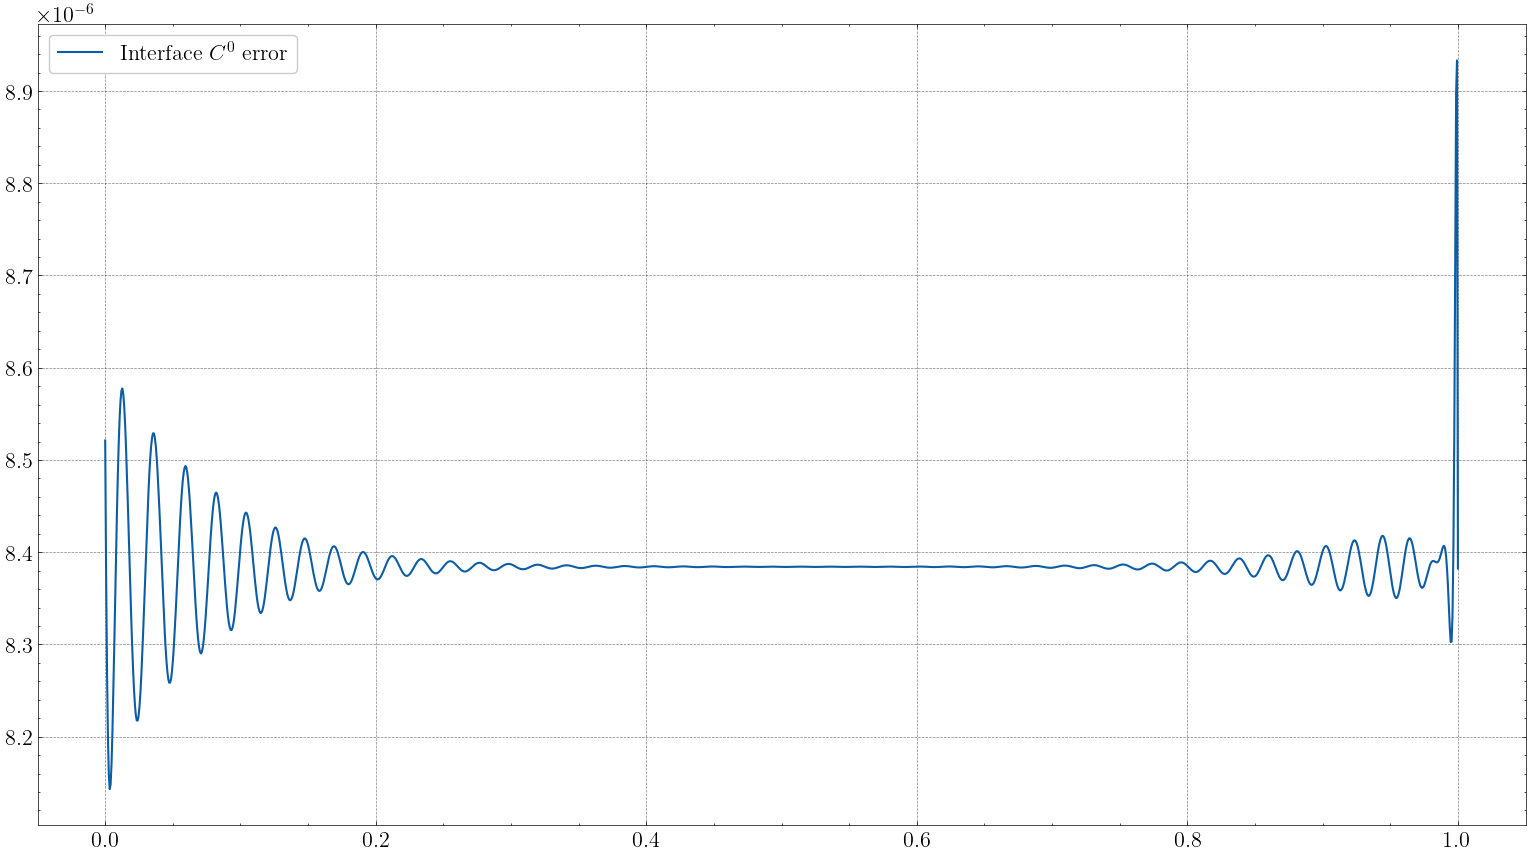
\includegraphics[width=1\linewidth]{Images/Transmission/L_shape_2_axis_c0_error_k1_2_enr.png}
      \caption{Interface \(C^0\) error}
      \label{transmission_L_axis_error_c0_k1_2}
    \end{minipage}%
    \begin{minipage}{.5\textwidth}
      \centering
      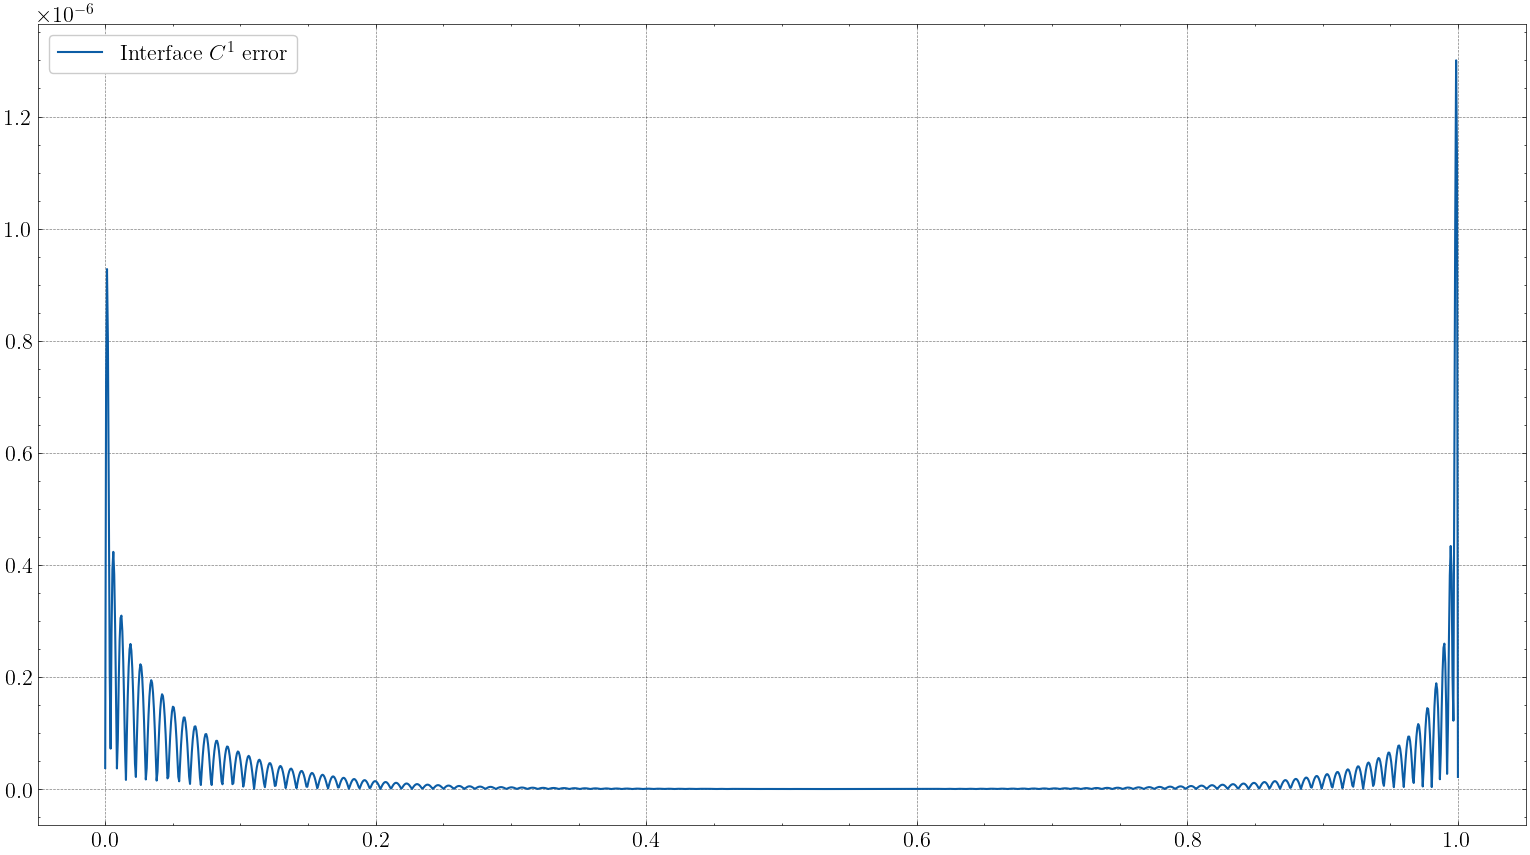
\includegraphics[width=1\linewidth]{Images/Transmission/L_shape_2_axis_c1_error_k1_2_enr.png}
      \caption{Interface \(C^0\) error}
      \label{transmission_L_axis_error_c1_k1_2}
    \end{minipage}
    
    \vspace{0.5cm} % Add some vertical space between the rows of figures
    
    \begin{minipage}{.6\textwidth}
      \centering
      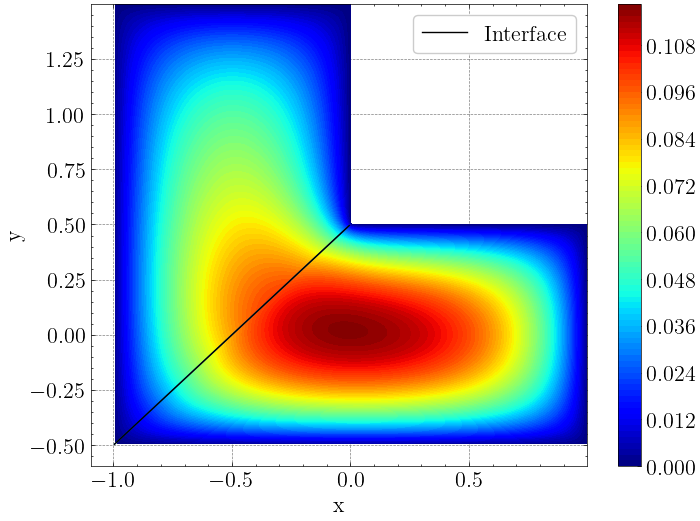
\includegraphics[width=\linewidth]{Images/Transmission/L_shape_2_axis_sol_k1_2_enr.png}
      %\caption{Numerical approximation}
      \label{transmission_L_axis_plot_k1_2}
    \end{minipage}
    
    \caption*{Absolute value of the interface errors and numerical approximation for \(k_1=2\), \(p_1=-2, -1, 0, 1\) and \(p_2 = 0, 1\).}
    \label{}
\end{figure}

Figures \ref{transmission_L_axis_error_c0_k1_2} and \ref{transmission_L_axis_error_c1_k1_2} show the absolute value of the errors for each interface point, with \(k_1=2\) and the \(p\) values for the particular solutions are \(p_1=-2, -1, 0, 1\) and \(p_2 = 0, 1\). As expected, both errors peak near the edges of the interface with special evidence when near the singular corner.
% If Printing on DOUBLE SIDED pages, the second page should be white.
% Otherwise, comment the following command:
%\cleardoublepage
%
%Chapter 5
% #############################################################################
% This is Chapter 5
% !TEX root = ../main.tex
% #############################################################################
% Change the Name of the Chapter i the following line
\fancychapter{The Poisson Equation with Variable Coefficients}
% \cleardoublepage
% The following line allows to ref this chapter
\label{chap:evaluation}

Lorem ipsum dolor sit amet, consectetuer adipiscing elit. Morbi commodo, ipsum sed pharetra gravida, orci magna rhoncus neque, id pulvinar odio lorem non turpis. Nullam sit amet enim. Suspendisse id velit vitae ligula volutpat condimentum. Aliquam erat volutpat. Sed quis velit. Nulla facilisi. Nulla libero. Vivamus pharetra posuere sapien. Nam consectetuer. Sed aliquam, nunc eget euismod ullamcorper, lectus nunc ullamcorper orci, fermentum bibendum enim nibh eget ipsum. Donec porttitor ligula eu dolor. Maecenas vitae nulla consequat libero cursus venenatis. Nam magna enim, accumsan eu, blandit sed, blandit a, eros. 
% #############################################################################
\section{Maecenas vitae nulla consequat} 
Aliquam aliquet, est a ullamcorper condimentum, tellus nulla fringilla elit, a iaculis nulla turpis sed wisi. Fusce volutpat. Etiam sodales ante id nunc. Proin ornare dignissim lacus. Nunc porttitor nunc a sem. Sed sollicitudin velit eu magna. Aliquam erat volutpat. Vivamus ornare est non wisi. Proin vel quam. Vivamus egestas. Nunc tempor diam vehicula mauris. Nullam sapien eros \Cref{fig:test_env}, facilisis vel, eleifend non, auctor dapibus, pede.

\begin{figure}[h]
\centering
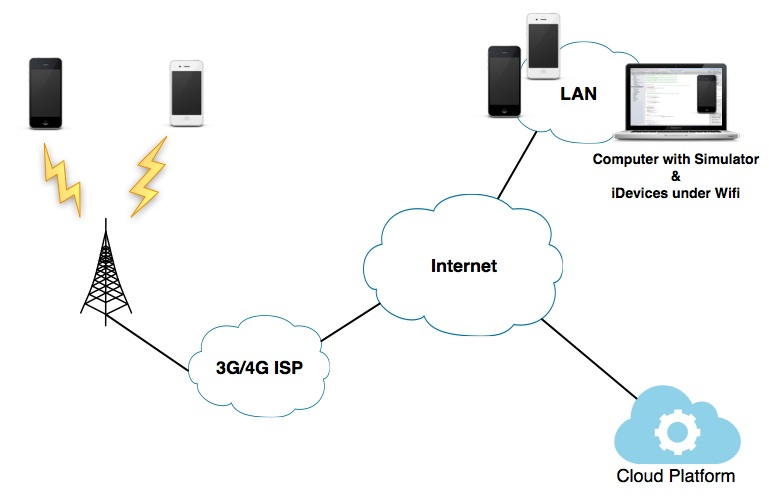
\includegraphics[width=0.8\textwidth]{./Images/test_env}
\caption{Test Environment}
\label{fig:test_env}
\end{figure}

Aliquam aliquet, est a ullamcorper condimentum, tellus nulla fringilla elit, a iaculis nulla turpis sed wisi. Fusce volutpat. Etiam sodales ante id nunc. Proin ornare dignissim lacus. Nunc porttitor nunc a sem. Sed sollicitudin velit eu magna. Aliquam erat volutpat. Vivamus egestas. Nunc tempor diam vehicula mauris. Nullam sapien eros, facilisis vel, eleifend non, auctor dapibus, pede \Cref{tab:network_profiles} used in the tests. The Network Link Conditioner allows to force/simulate fluctuations in fixed network segments.

\begin{table}[htb]
\centering
\normalsize
    \caption{Network Link Conditioner Profiles}
    \label{tab:network_profiles}
{\footnotesize
    \begin{tabular}{ | c | c | c | c | }
    \hline 
    \textbf{Network Profile}	& \textbf{Bandwidth} & \textbf{Packets Droped} & \textbf{Delay}\\ \hline \hline
    Wifi  & 40 mbps  &  0\%  &   1 ms \\ \hline
    3G  & 780 kbps  &  0\%  &   100 ms \\ \hline 
    Edge  & 240 kbps  &  0\%  &   400 ms \\ \hline
    \end{tabular}
    }
\end{table}

Aliquam aliquet, est a ullamcorper condimentum, tellus nulla fringilla elit, a iaculis nulla turpis sed wisi. Fusce volutpat. Etiam sodales ante id nunc. Proin ornare dignissim lacus. Nunc porttitor nunc a sem. Sed sollicitudin velit eu magna. Aliquam erat volutpat. Vivamus ornare est non wisi. Proin vel quam. Vivamus egestas. Nunc tempor diam vehicula mauris. Nullam sapien eros, facilisis vel, eleifend non, auctor dapibus, pede.
% #############################################################################
\section{Proin ornare dignissim lacus}
Pellentesque habitant morbi tristique senectus et netus et malesuada fames ac turpis egestas. Vestibulum tortor quam, feugiat vitae, ultricies eget, tempor sit amet, ante. Donec eu libero sit amet quam egestas semper. Aenean ultricies mi vitae est. Mauris placerat eleifend leo. Quisque sit amet est et sapien ullamcorper pharetra. Vestibulum erat wisi, condimentum sed, commodo vitae, ornare sit amet, wisi. Aenean fermentum, elit eget tincidunt condimentum, eros ipsum rutrum orci, sagittis tempus lacus enim ac dui. Donec non enim in turpis pulvinar facilisis. Ut felis.

Et ``optimistic'' nulla dui purus, eleifend vel, consequat non, dictum porta, nulla. Duis ante mi, laoreet ut, commodo eleifend, cursus nec, lorem. Aenean eu est. Etiam imperdiet turpis. Praesent nec augue. Curabitur ligula quam, rutrum id, tempor sed, consequat ac, dui $G_j$, nec ligula et lorem consequat ullamcorper $p$ ut mauris eu mi mollis luctus $j$, porttitor ut, \Cref{unchoke_gain}, uctus posuere justo:

\begin{description}
  \item[$N_j$] Is the number of times peer $j$ has been optimistically unchoked.
  \item[$n_j$] Among the $N_j$ unchokes, the number of times that peer $j$ responded with unchoke or supplied segments to peer $p$.
  \item[$C_{r[j]}$] The cooperation ratio of peer $j$. If peer $j$ never supplied peer $p$, the information of $C_{r[j]}$ may not be available.
  \item[$C_{r (max)}$] The maximum cooperation ratio of peer $p$’s neighbors, i.e., $C_{r (max)} = max(C_r)$.
\end{description}

\begin{equation}
\label{unchoke_gain}
 G_j =
  \begin{dcases}
    \frac{n_j C_{r[j]}}{N_j} &\quad \text{if } n_j > 0\\
    \frac{C_{r (max)}}{N_j + 1} &\quad \text{if } n_j = 0
  \end{dcases}
\end{equation}

Cursus $C_{r (max)}$ conubia nostra, per inceptos hymenaeos $j$ gadipiscing mollis massa $N_j = 0$, unc ut dui eget nulla venenatis aliquet $G_j = C_{r (max)}$.

Vestibulum accumsan eros nec magna. Vestibulum vitae dui. Vestibulum nec ligula et lorem consequat ullamcorper. Class aptent taciti sociosqu ad litora torquent per conubia nostra, per inceptos hymenaeos. Phasellus eget nisl ut elit porta ullamcorper. Maecenas tincidunt velit quis orci. Sed in dui. Nullam ut mauris eu mi mollis luctus. Class aptent taciti sociosqu ad litora torquent per conubia nostra, per inceptos hymenaeos. Sed cursus cursus velit. Sed a massa. 

Both \Cref{fig:tx_layer_4,fig:tx_layer_5} Phasellus eget nisl ut elit porta ``perfect'' tincidunt. Class aptent taciti sociosqu ad litora torquent per conubia nostra.

\begin{figure}[h]
%\centering
       \subfigure[Adaptation System Test 4]{\label{fig:tx_layer_4}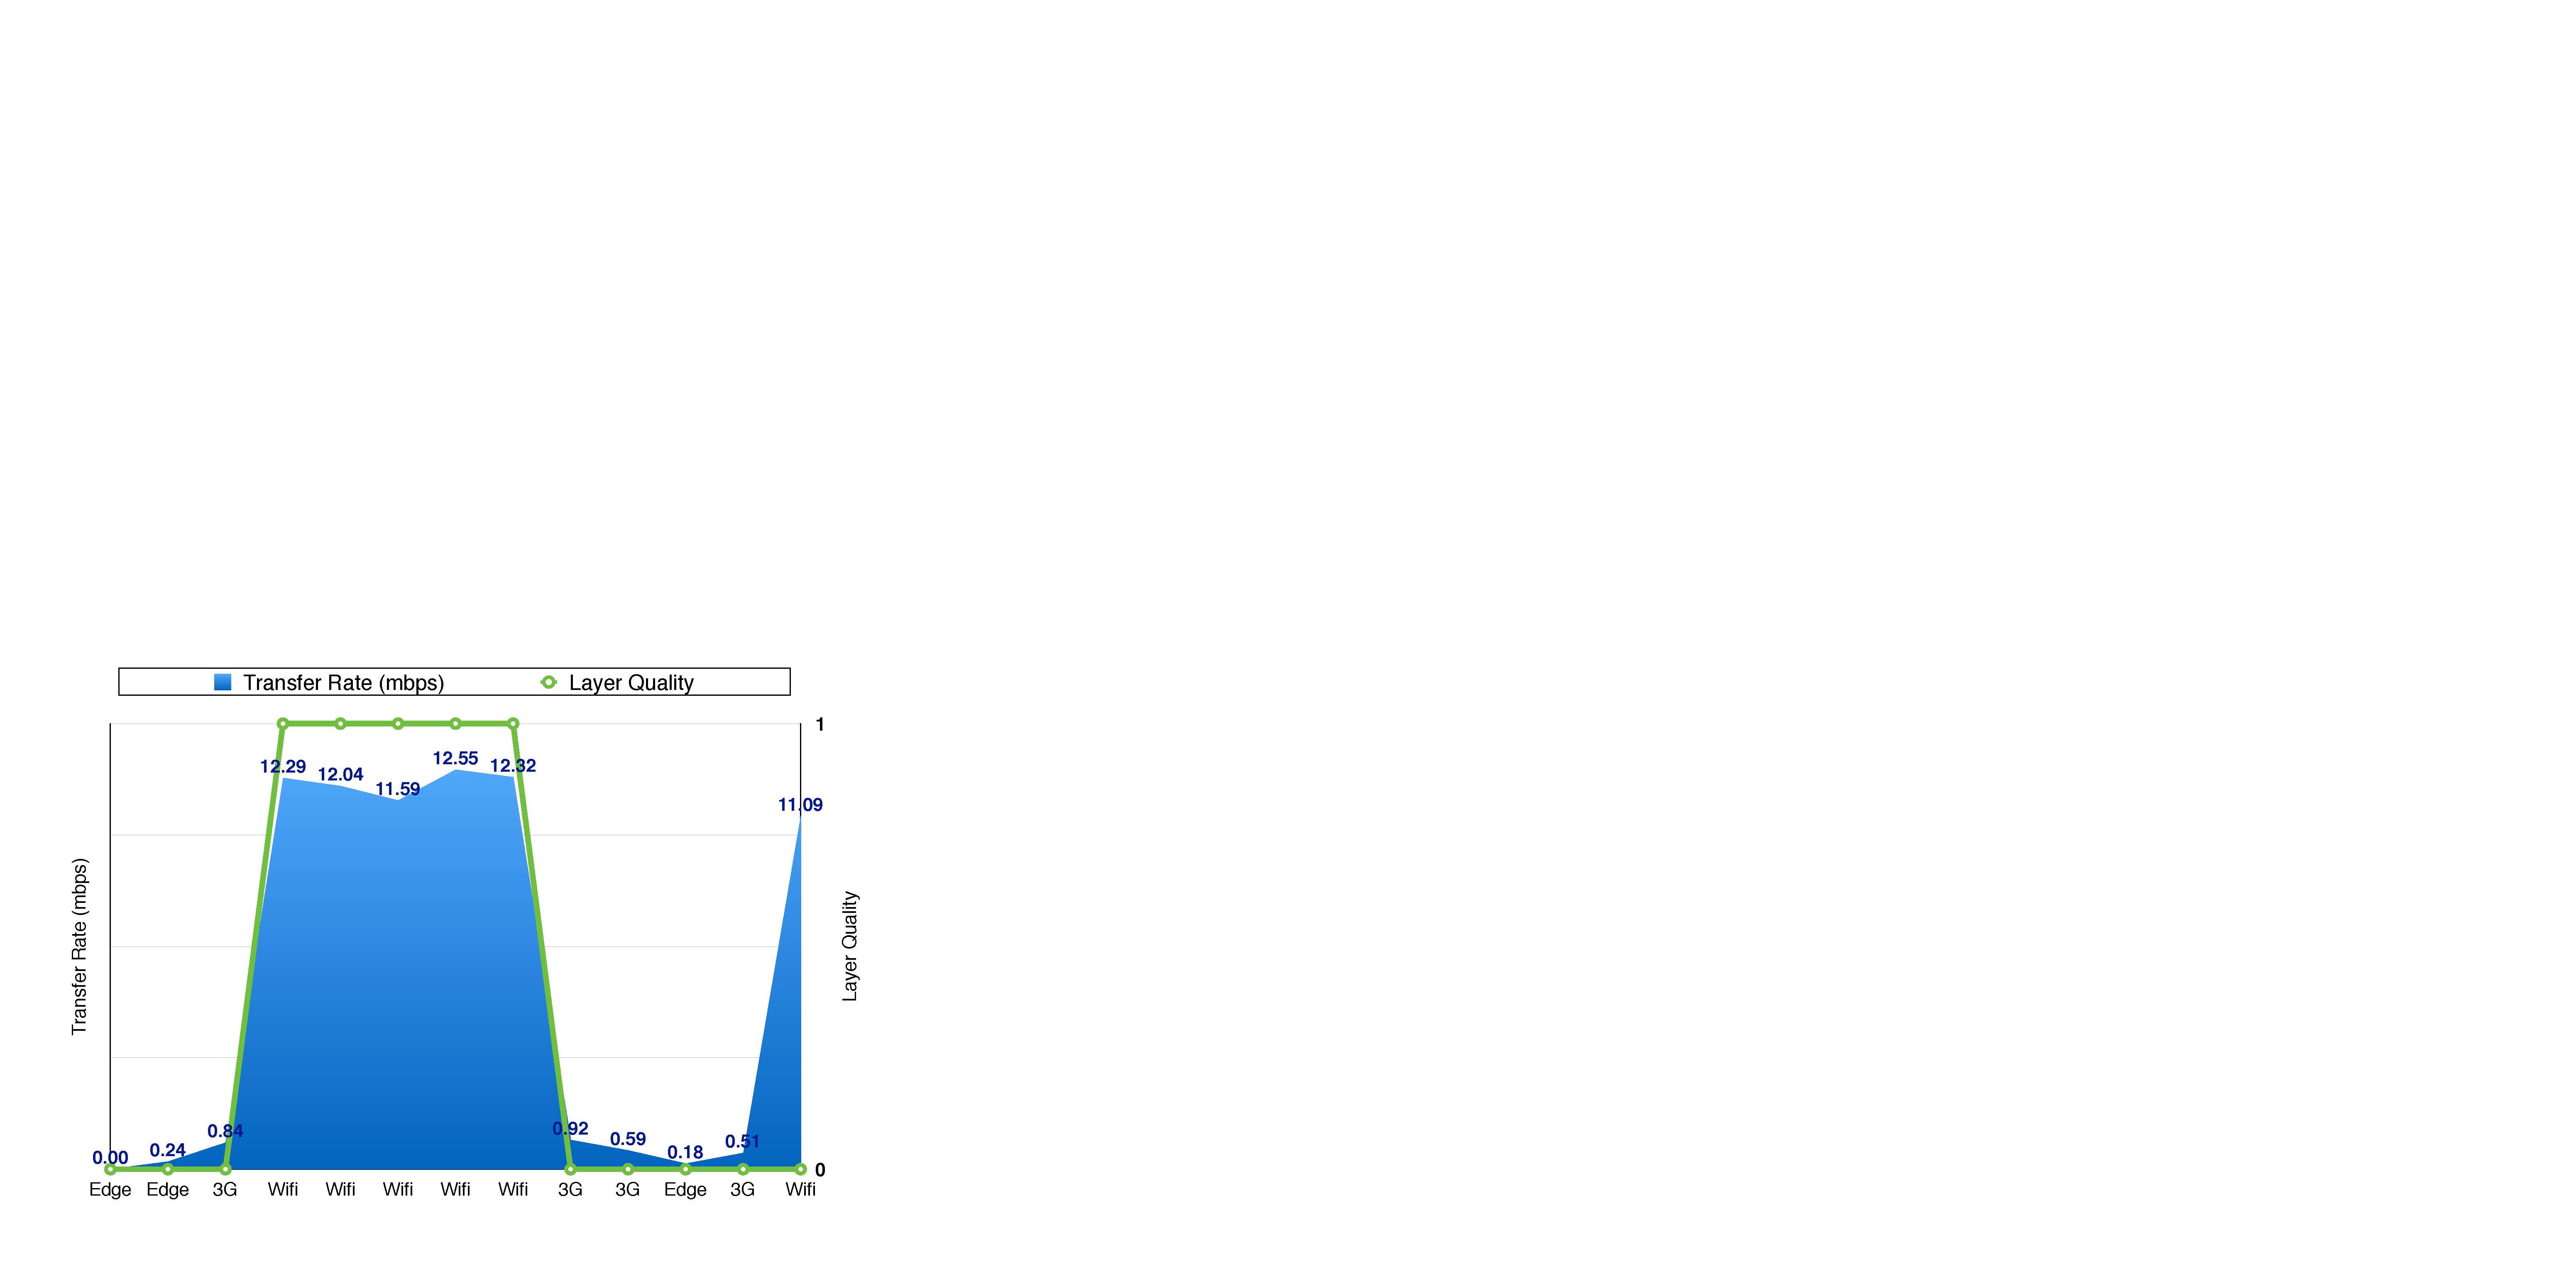
\includegraphics[width=0.5\textwidth]{./Images/tx_layer_4}}  
   %    \centering 
       \subfigure[Adaptation System Test 5]{\label{fig:tx_layer_5}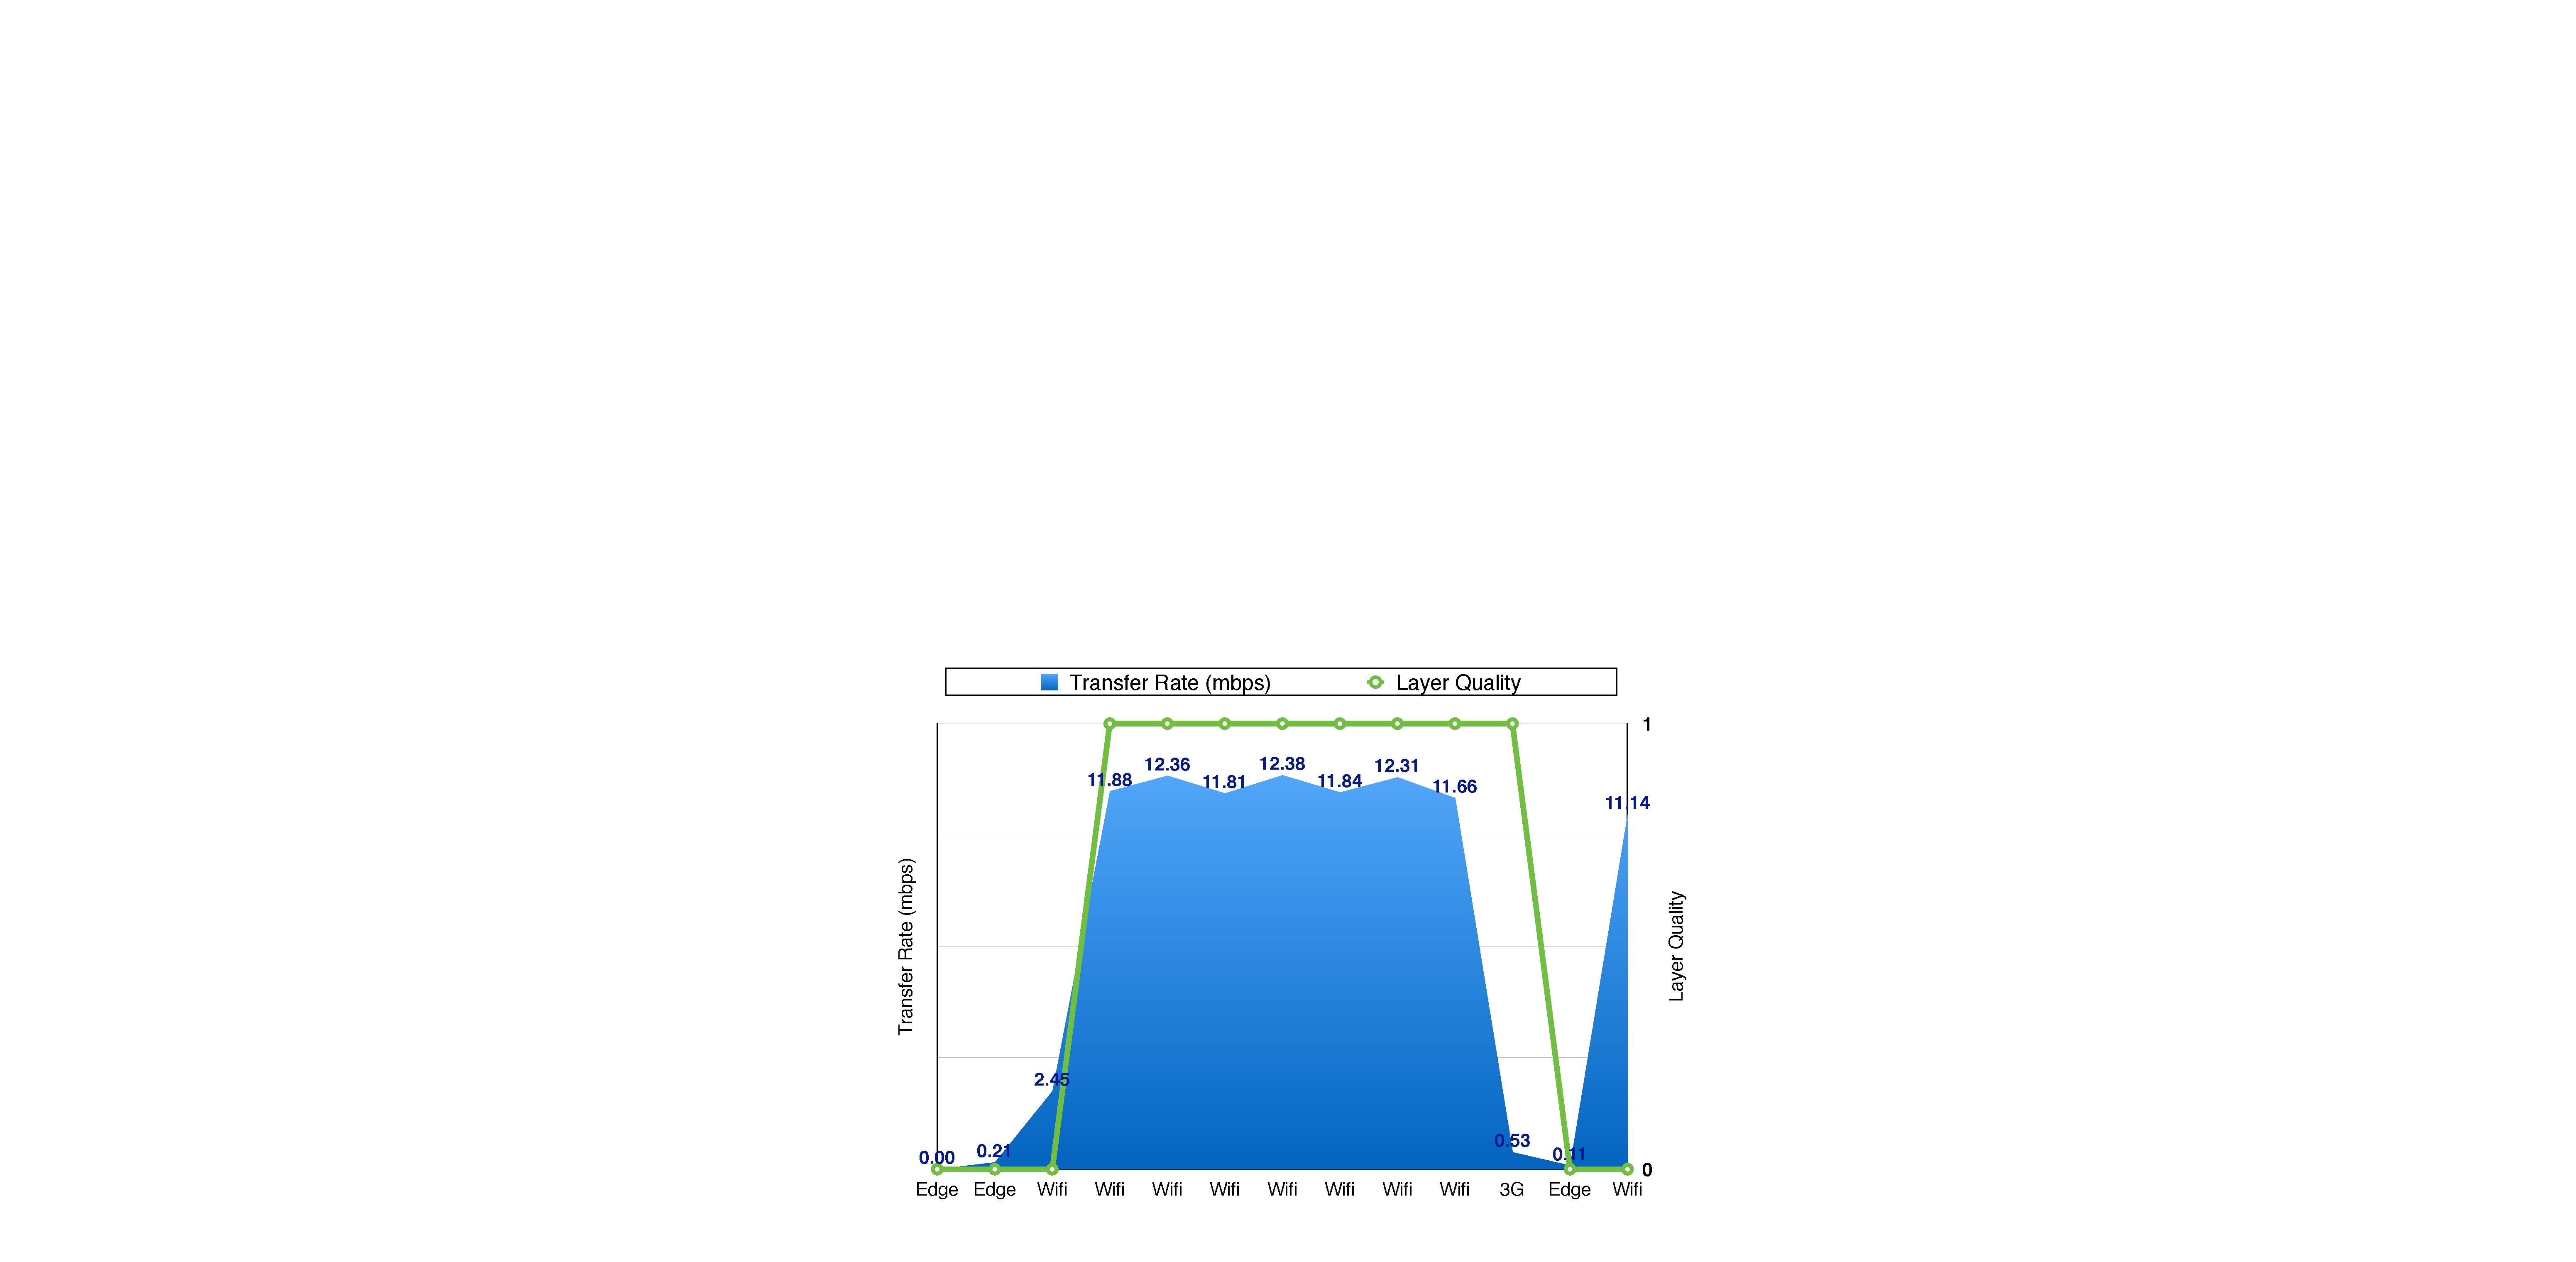
\includegraphics[width=0.5\textwidth]{./Images/tx_layer_5}}   
        \caption{Adaptation System Behavior Test}
        \label{fig:fig:adapt_behave_2}
\end{figure}

Cras sed ante. Phasellus in massa. Curabitur dolor eros, gravida et, hendrerit ac, cursus non, massa. Aliquam lorem. In hac habitasse platea dictumst. Cras eu mauris. Quisque lacus. Donec ipsum. Nullam vitae sem at nunc pharetra ultricies. Vivamus elit eros, ullamcorper a, adipiscing sit amet, porttitor ut, nibh. Maecenas adipiscing mollis massa. Nunc ut dui eget nulla venenatis aliquet. Sed luctus posuere justo. Cras vehicula varius turpis. Vivamus eros metus, tristique sit amet, molestie dignissim, malesuada et, urna.

% If Printing on DOUBLE SIDED pages, the second page should be white.
% Otherwise, comment the following command:
%\cleardoublepage
%
%Chapter 6
% #############################################################################
% This is Chapter 6
% !TEX root = ../main.tex
% #############################################################################
% Change the Name of the Chapter i the following line
\fancychapter{Conclusion}
% \cleardoublepage
% The following line allows to ref this chapter
\label{chap:conclusion}

 Pellentesque vel dui sed orci faucibus iaculis. Suspendisse dictum magna id purus tincidunt rutrum. Nulla congue. Vivamus sit amet lorem posuere dui vulputate ornare. Phasellus mattis sollicitudin ligula. Duis dignissim felis et urna. Integer adipiscing congue metus\todo[color=green!40, author=Rui Cruz, fancyline]{You should always start a Chapter with an introductory text}{}.
% #############################################################################
\section{Conclusions}
Lorem ipsum dolor sit amet, consectetuer adipiscing elit. Morbi commodo, ipsum sed pharetra gravida, orci magna rhoncus neque, id pulvinar odio lorem non turpis. Nullam sit amet enim. Suspendisse id velit vitae ligula volutpat condimentum. Aliquam erat volutpat. Sed quis velit. Nulla facilisi. Nulla libero. Vivamus pharetra posuere sapien. Nam consectetuer. Sed aliquam, nunc eget euismod ullamcorper, lectus nunc ullamcorper orci, fermentum bibendum enim nibh eget ipsum. Donec porttitor ligula eu dolor. Maecenas vitae nulla consequat libero cursus venenatis. Nam magna enim, accumsan eu, blandit sed, blandit a, eros.

Quisque facilisis erat a dui. Nam malesuada ornare dolor. Cras gravida, diam sit amet rhoncus ornare, erat elit consectetuer erat, id egestas pede nibh eget odio. Proin tincidunt, velit vel porta elementum, magna diam molestie sapien, non aliquet massa pede eu diam. Aliquam iaculis. Fusce et ipsum et nulla tristique facilisis. Donec eget sem sit amet ligula viverra gravida. Etiam vehicula urna vel turpis. Suspendisse sagittis ante a urna. Morbi a est quis orci consequat rutrum. Nullam egestas feugiat felis. Integer adipiscing semper ligula. Nunc molestie, nisl sit amet cursus convallis, sapien lectus pretium metus, vitae pretium enim wisi id lectus. Donec vestibulum. Etiam vel nibh. Nulla facilisi. Mauris pharetra. Donec augue. Fusce ultrices, neque id dignissim ultrices, tellus mauris dictum elit, vel lacinia enim metus eu nunc.

Proin at eros non eros adipiscing mollis. Donec semper turpis sed diam. Sed consequat ligula nec tortor. Integer eget sem. Ut vitae enim eu est vehicula gravida. Morbi ipsum ipsum, porta nec, tempor id, auctor vitae, purus. Pellentesque neque. Nulla luctus erat vitae libero. Integer nec enim. Phasellus aliquam enim et tortor. Quisque aliquet, quam elementum condimentum feugiat, tellus odio consectetuer wisi, vel nonummy sem neque in elit. Curabitur eleifend wisi iaculis ipsum. Pellentesque habitant morbi tristique senectus et netus et malesuada fames ac turpis egestas. In non velit non ligula laoreet ultrices. Praesent ultricies facilisis nisl. Vivamus luctus elit sit amet mi. Phasellus pellentesque, erat eget elementum volutpat, dolor nisl porta neque, vitae sodales ipsum nibh in ligula. Maecenas mattis pulvinar diam. Curabitur sed leo.

Nulla facilisi. In vel sem. Morbi id urna in diam dignissim feugiat. Proin molestie tortor eu velit. Aliquam erat volutpat. Nullam ultrices, diam tempus vulputate egestas, eros pede varius leo, sed imperdiet lectus est ornare odio. Lorem ipsum dolor sit amet, consectetuer adipiscing elit. Proin consectetuer velit in dui. Phasellus wisi purus, interdum vitae, rutrum accumsan, viverra in, velit. Sed enim risus, congue non, tristique in, commodo eu, metus. Aenean tortor mi, imperdiet id, gravida eu, posuere eu, felis. Mauris sollicitudin, turpis in hendrerit sodales, lectus ipsum pellentesque ligula, sit amet scelerisque urna nibh ut arcu. Aliquam in lacus. Vestibulum ante ipsum primis in faucibus orci luctus et ultrices posuere cubilia Curae; Nulla placerat aliquam wisi. Mauris viverra odio. Quisque fermentum pulvinar odio. Proin posuere est vitae ligula. Etiam euismod. Cras a eros.

Nunc auctor bibendum eros. Maecenas porta accumsan mauris. Etiam enim enim, elementum sed, bibendum quis, rhoncus non, metus. Fusce neque dolor, adipiscing sed, consectetuer et, lacinia sit amet, quam.
% #############################################################################
\section{System Limitations and Future Work}
Aliquam aliquet, est a ullamcorper condimentum, tellus nulla fringilla elit, a iaculis nulla turpis sed wisi. Fusce volutpat. Etiam sodales ante id nunc. Proin ornare dignissim lacus. Nunc porttitor nunc a sem. Sed sollicitudin velit eu magna. Aliquam erat volutpat. Vivamus ornare est non wisi. Proin vel quam. Vivamus egestas. Nunc tempor diam vehicula mauris. Nullam sapien eros, facilisis vel, eleifend non, auctor dapibus, pede.
% If Printing on DOUBLE SIDED pages, the second page should be white.
% Otherwise, comment the following command:
%\cleardoublepage
%
% -----------------------------------------------------------------------------
% BIBLIOGRAPHY
% Add the Bibliography to the PDF table of contents (not the document table of contents)
%\pdfbookmark[0]{Bibliography}{bib}
\addcontentsline{toc}{chapter}{Bibliography}
% The bibliography style sheet
% Chose your preferences on the format of the entries and the Labels:
% IEEEtran: Used in general (recommended for IST Thesis)
%           Entries are labelled and sorted by appearance in the document
%           Labels are Numeric inside square brackets
\bibliographystyle{IEEEtran}
%
% Apalike:  Entries formatted alphabetically, last name first, with identation
%           Labels with Autor's Name and Year inside square brackets
%\bibliographystyle{apalike}
%
% Alpha:    Entries formatted with Autor's Name and Year, hanging identation
%           Labels with Autor's abbr. Names and Year inside square brackets
%\bibliographystyle{alpha}
%
% Acm:     Entries formatted with Autor's Name (small Caps), hanging identation
%          Labels are Numeric inside square brackets
%\bibliographystyle{acm}
% The following command resets the 'emphasis' style for bibliography entries
\normalem
% Name of your BiBTeX file
\bibliography{Thesis-MSc-Bibliography} % Put here your own filename
%
% The following command modifies the 'emphasis' style for bibliography entries
\ULforem
% If Printing on DOUBLE SIDED pages, the second page should be white.
% Otherwise, comment the following command:
%\cleardoublepage
%
% -----------------------------------------------------------------------------
% Glossary
%\newglossaryentry{Hahn-Banach Theorem}{
    name={Hahn-Banach Theorem},
    description={A fundamental result in functional analysis}
}
\printglossary[] \mtcaddchapter

% If Printing on DOUBLE SIDED pages, the second page should be white.
%\clearpage
% Otherwise, comment the following command:
%\cleardoublepage
% -----------------------------------------------------------------------------
% HERE GO THE APPENDIXES IF REQUIRED
% If not required just comment the blocks
\appendix
%% First Appendix
%\pdfbookmark[1]{Appendix A}{appendix}
% #############################################################################
% This is Appendix A
% !TEX root = ../main.tex
% #############################################################################
\chapter{Spectral Decomposition of the Laplace operator}\label{div_theo}

% In this appendix, some concepts in Hilbert spaces are presented and applied to the Laplace operator. While they could also be presented in the first Chapter, the results presented here are classical and are not used in the theoretical justification of the \ac{MFS}.

% \section{Some concepts on Hilbert spaces}
% % For more details c.f \cite{rudin1991functional}, \cite{brezis2011functional}, \cite{arendt2010partielle}.
% In this section, we introduce some complementary results in Hilbert spaces. Once again, for more details, see \cite{rudin1991functional}, \cite{brezis2011functional}, or \cite{arendt2010partielle}. Consider the field \(\mathbb{F}\) (\(\mathbb{R}\) or \(\mathbb{C}\)). We say that a vector space \(H\) is an \textit{inner product space} (or a Pre-Hilbert space) if there exists a map \((\cdot,\cdot)\) (called an \textit{inner product}) over \(\mathbb{F}\) such that
% \begin{enumerate}
%     \item \((x, y) = \overline{(y, x)}\) (The bar denotes complex conjugation if \(\mathbb{F} = \mathbb{C}\));
%     \item \((x+y,z) = (x,z)+(y+z)\);
%     \item \((\alpha x, y)=\alpha(x, y)\), \(\alpha \in \mathbb{F}\);
%     \item \((x, x) \geq 0, \; \forall x \in H\);
%     \item \((x, x) = 0 \iff x=0\).
% \end{enumerate}
% Given \(x, y \in H\), we say that \(x\) and \(y\) are orthogonal (denoted by \(x \perp y\)) if \((x, y) = 0\). Accordingly, given \(E, F \subset H\), if \(x\perp y\) for every \(x \in E, y \in F\) then we say that \(E\) and \(F\) are orthogonal, \(E \perp F\). We also denote by \(E^\perp\) the set of all \(y \in H\) that are orthogonal to every \(x \in E\), i.e., \(E^\perp = \{y \in H: (x, y)=0, \; \forall x \in E\}\) which we call the orthogonal complement of \(E\). We recall that every inner product space is also a normed space, where the inner product induces the norm
% \[
% \norm*{x} = \sqrt{(x, x)}   
% \]
% satisfying the Cauchy-Schwarz inequality
% \[
% \abs{(x, y)} \leq \norm*{x}\norm*{y}, \; x, y \in H.
% \]
% Finally, if the normed space is complete for the induced norm, then we say that it is a Hilbert space. In what follows, \(H\) will always denote a Hilbert space.
% \begin{example}
%     A very classical Hilbert space, which is going to be used throughout all of this work, is the space of square-integrable real-valued functions in an open and bounded subset \(\Omega\) of \(\mathbb{R}^d\), which is denoted by \(L^2(\Omega)\) with the inner product given by
%     \[
%     (f, g)_{L^2(\Omega)} = \int_\Omega f(x)g(x) dx.
%     \]
%     If considering complex-valued functions, the inner product is given by
%     \[
%         (f, g)_{L^2(\Omega)} = \int_\Omega f(x)\overline{g}(x) dx,
%     \]
%     where a bar over an expression represents the complex conjugate of the scalar (function).
% \end{example}
% While working within the framework of Hilbert spaces, proving the density of a subspace \(M \subset H\) is more intuitive and can be derived straightforwardly. It may be of interest to the reader to compare the following results with Definition \eqref{banach_ortho_def} and Lemma \ref{banach_ortho_lemma}.
% \begin{theorem}\label{hilb_decomp}
%     Consider a closed subspace \(M \subset H\). Then,
%     \[
%     H = M \oplus M^\perp.
%     \]
%     In other words, every \(u \in H\) admits a unique decomposition \(u = v + w\), where \(v \in M\) and \(w \in M^\perp\).
% \end{theorem}
% \begin{corollary}\label{hilb_dense}
%     Consider a subspace \(M \subset H\). Then \(M\) is dense in \(H\) if and only if \(M^\perp = \{0\}\).
% \end{corollary}
% \begin{proof}
%     Let \(T = \overline{M}\). We want to prove that \(T = H\). Using Theorem \ref{hilb_decomp}, it suffices to check that \(T^\perp = \{0\}\). Since the inner product is continuous, then \(T^\perp = M^\perp = \{0\}\).
    
%     On the other hand, since by definition \(T\) is closed, by Theorem \ref*{hilb_decomp} we have that \(H = T \oplus T^\perp = T \oplus \{0\} = T\) as we wished.
% \end{proof}
% A surprising property in Hilbert spaces is the fact that every linear and continuous function \(T: H \rightarrow \mathbb{F}\) can be \textit{represented} by some unique element in \(H\). In what follows we assume that \(\mathbb{F} = \mathbb{R}\).
% \begin{theorem}[Riesz Representation Theorem]\label{riesz}
%     Let \(T: H \rightarrow \mathbb{R}\) be a linear and continuous functional. Then, there exists a unique \(u \in H\) such that
%     \[
%         T v = (u, v), \; \forall v \in H.
%     \]
%     Moreover, let \(H^\star\) be the dual space of \(H\), that is, the space of all linear and continuous functions from \(H\) to \(\mathbb{R}\). Then the map \(H^\star \mapsto H\) is an isometric isomorphism (which we denote by \(\approxeq\)) where
%     \[
%         \norm*{u}_H = \norm*{T}_{H^\star}.
%     \]
% \end{theorem} 
% \begin{remark}
%     Notice how the inner product in Hilbert spaces has replaced the duality pairing defined for Banach spaces. In fact, in a certain sense, Riesz Representation Theorem \ref{riesz} allows us to make a stronger statement regarding the dual spaces of Hilbert spaces and work in a more natural framework without ever resorting to the Hahn-Banach Theorem \ref{hb_ana_form}. For example, it is interesting to observe that the definition of orthogonality and orthogonal subspaces in Hilbert spaces (via the inner product) and Banach spaces (via the duality pairing) are essentially the same, with the distinction being an isomorphism between the Hilbert space and its dual. However, in certain cases, working with the definition of orthogonality in Banach spaces can be more useful as it allows for better generalization, such as when proving the density of a closed subspace.
% \end{remark}
% A more general and useful result in our work is the Lax-Milgram Theorem.
% \begin{definition}
%     We say that a bilinear form \(a: H \times H \rightarrow \mathbb{R}\) is continuous and coercive if
%     \begin{itemize}
%         \item \(\abs{a(u,v)} \leq C \norm*{u}\norm*{v}, \; \forall u, v \in H\)
%         \item \(a(u,u) \geq \alpha \norm*{u}^2, \; \forall u \in H\)
%     \end{itemize}
%     respectively.
% \end{definition}
% \begin{theorem}[Lax-Milgram Theorem]\label{lax-milgram}
%     Let \(a(u,v)\) be a bilinear, continuous, and coercive bilinear form on \(H\). If \(T\) is a linear and continuous functional in \(H\), then there exists a unique \(u \in H\) such that
%     \[
%         a(u, v) = T(v), \; \forall v \in H.
%     \]
% \end{theorem}
% In this section, the well-known \textit{Spectral Theorem} is presented. With this in mind, we will now present key results and concepts (without proof) that will provide the necessary foundation for stating the theorems.
% \begin{definition}
%     A sequence \((e_n)_{n \in \mathbb{N}} \in H\) is a Hilbert basis of \(H\) if
%     \begin{enumerate}
%         \item \((e_n, e_m) = \begin{cases}
%             1, & n=m\\
%             0, & n \neq m
%         \end{cases}\);
%         \item \(\overline{\Span\{(e_n)_{n \in \mathbb{N}}\}} = H\).
%     \end{enumerate}
% \end{definition}
% In a sense, a Hilbert basis resembles a basis in a finite-dimensional vector space.
% \begin{proposition}\label{hilb_basis}
%     Let $(e_n)_{n \in \mathbb{N}}$ be a Hilbert basis of $H$. Then, for every $u \in H$, we can write
%     \[
%         u = \sum_{k \in \mathbb{N}} (u, e_k)e_k \quad \text{and} \quad \|u\|^2 = \sum_{k \in \mathbb{N}} |(u, e_k)|.
%     \]
%     The last equality is known as \textit{Parseval's identity}.
% \end{proposition}
% The proposition above is particularly interesting because it allows us to express every element of \(H\) in terms of a countable basis. The following result guarantees the existence of a Hilbert basis if certain conditions are met.
% \begin{definition}
%     We say that \(H\) is a separable Hilbert space if there exists a countable subset \(M \subset H\) such that \(\overline{M} = H\).
% \end{definition}
% \begin{theorem}
%     Every separable Hilbert space admits an orthonormal Hilbert basis.
% \end{theorem}

% We now present some properties that our operators must satisfy in order to state the Spectral Theorem.
% \begin{definition}
%     Consider a linear operator \(T: H_1 \rightarrow H_2\), where \(H_1\) and \(H_2\) are Hilbert spaces.
%     \begin{enumerate}
%         \item Assume that \(H = H_1=H_2\) and \(T \in \mathcal{L}(H)\). We say that \(T^\star\) is the \textbf{adjoint} of \(T\) if
%         \[
%         (y, T x) = (T^\star y, x), \; \forall x, y \in H;
%         \]
%         If \(T=T^\star\), i.e., if \(T\) and \(T^\star\) domains (and their image) coincide we say that \(T\) is \textbf{self-adjoint}.\footnote{The existence and uniqueness of \(T^\star\) may not be obvious, but if follows from Riesz Representation Theorem \ref{riesz}. In any case, notice the similarities between this definition and the one given in Definition \eqref{banach_op_def}. In fact, in Banach spaces, the existence of the adjoint also comes from the Hahn-Banach Theorem \ref{hb_ana_form}!}
%         \item As above, let \(T \in \mathcal{L}(H)\). We say that \(\lambda\) is an \textbf{eigenvalue} of \(T\) if \(N(T - \lambda I) \neq \{0\}\). In that case, we say that \(\lambda \in \sigma(T)\) where \(\sigma(T)\) is called the \textbf{spectrum} of \(T\)\footnote{Remarkably, in the infinite-dimensional case, the set of eigenvalues \(EV(T)\) may not coincide with the spectrum \(\sigma(T)\). \(T - \lambda I\) may fail to be invertible even if \(T - \lambda I\) is injective.}. We also say that \(u\) is an \textbf{eigenvector} associated with the eigenvalue \(\lambda\) if \(u \in N(T-\lambda I)\setminus \{0\}\).
%     \end{enumerate}
% \end{definition}
% We can derive some important properties regarding the spectrum of a compact operator and the spectrum of self-adjoint operators.
% \begin{proposition}
%     Let \(H\) be a Hilbert space and consider a compact operator \(T \in \mathcal{L}(H)\). Then,
%     \begin{itemize}
%         \item \(0 \in \sigma(T)\);
%         \item one of the following holds:
%         \begin{itemize}
%             \item \(\sigma(T) = \{0\}\);
%             \item \(\sigma(T)\setminus\{0\}\) is a finite set;
%             \item \(\sigma(T)\setminus\{0\}\) is a sequence converging to \(0\).
%         \end{itemize} 
%     \end{itemize}
% \end{proposition}
% \begin{proposition}
%     Let \(H\) be a Hilbert space and consider a self-adjoint operator \(T\in \mathcal{L}(H)\). In these conditions, \(\sigma(T)\) is real and eigenvectors corresponding to distinct eigenvalues are orthogonal.
% \end{proposition}
% It is now possible to state one of the main results of this section.
% \begin{theorem}[Spectral Theorem for compact and self-adjoint operators]\label{spectral_theorem}
%     Let \(H\) be a separable Hilbert space of infinite dimension and let \(T \in \mathcal{L}(H)\) be a compact self-adjoint operator. Then, \(H\) admits a Hilbert basis \((e_n)_{n \in \mathbb{N}}\) such that
%     \[
%         T e_n = \lambda_n e_n
%     \]
%     for \(\lambda_n \in \mathbb{R}\), \(\lambda_n \rightarrow 0\) as \(n \rightarrow \infty\), where \(\lambda_n\) can be assumed to be a decreasing sequence.
% \end{theorem}

%\section{Spectral Decomposition of the Laplace operator}\label{div_theo}

In this appendix, we make a brief study regarding the Laplace operator in a bounded domain \(\Omega \subset \mathbb{R}^d\) with Lipschitz boundary. The main results presented here are mostly consequences of the Spectral Theorem \ref{spectral_theorem}. Firstly, recall the Divergence Theorem, e.g. \cite{evans2015measure}.

\begin{theorem}[Divergence Theorem]\label{appendix_div_theor}
    Let \(\Omega \subset \mathbb{R}^d\) defined as above. Then,
    \[
      \int_\Omega \Div \phi dx = \int_{\partial\Omega} \phi \cdot \mathbf{n} d\sigma,
    \]
    where \(\mathbf{n}\) denotes the exterior unitary normal and the \((d-1)\)-surface element is given by
    \[
        d\sigma = \sqrt{1+ \abs{\nabla \varphi_i}^2} d \mathbf{y}'
    \]
    where \(\varphi\) is the local parametrization given in Definition \ref{ck_lipschitz_domains_def}\footnote{Although \(\varphi\)} is only a Lipschitz function, by Rademacher Theorem (see Chapter 1 in \cite{salsa2016partial}) \(\varphi\) is differentiable almost everywhere.
\end{theorem}

A main consequence of the Divergence Theorem are the well-known \textit{Green's Formulas}.
\begin{corollary}[Green's Formulas]
    In this same conditions of the Theorem \ref{appendix_div_theor}, let \(u, v \in H^2(\Omega)\). Then,
    \begin{enumerate}
        \item \(\int_\Omega \Delta u dx = \int_{\partial \Omega} \frac{\partial u}{\partial n} d\sigma\);
        \item \(\int_\Omega \Delta u v dx = -\int_\Omega \nabla u \cdot \nabla v dx + \int_{\partial \Omega} \frac{\partial u}{\partial n}v d\sigma\);
        \item \(\int_\Omega \Delta u v - u \Delta v dx= \int_{\partial \Omega} \frac{\partial u}{\partial n}v - \frac{\partial v}{\partial n}u d\sigma\).
    \end{enumerate}
\end{corollary}

The study of the spectrum of the Laplace operator is of major importance in this work. We will only state and prove a classical result which can also be found in numerous textbooks, see \cite{brezis2011functional}, \cite{arendt2010partielle}, \cite{courant2008methods} or \cite{borthwick2020spectral}. While we assume null Dirichlet boundary conditions, we notice that the Neumann case is analogous.

\begin{definition}\label{eig_def}
    Consider the Helmholtz equation with null Dirichlet boundary conditions
    \begin{equation}\label{eig_helm_eq}
        \begin{cases}
            -\Delta u(x) = \lambda u(x), & x \in \Omega, \\
            u(x) = 0, & x \in \partial \Omega.
        \end{cases}
    \end{equation}
    One says that \(\lambda \in \mathbb{C}\) is an eigenvalue of the equation \eqref{eig_helm_eq} if there exists an eigenfunction \(u \neq 0\) belonging to the function spaces \(C^2(\Omega) \cap C(\overline{\Omega})\).
\end{definition}

\begin{theorem}\label{spec_lap_pre}
    There exists a Hilbert basis \((u_n)_{n \in \mathbb{N}}\) of \(L^2(\Omega)\) consisting of eigenfunctions \(u_n\) of \(-\Delta\), i.e., for each \(n \in \mathbb{N}\) there exists a pair eigenvalue/eigenfunction \((\lambda_n, u_n)\) such that
    \[
        -\Delta u_n = \lambda_n u_n
    \]
    where the sequence of eigenvalues can be ordered in increasing order and \(\lambda_n \rightarrow \infty, \; n \rightarrow \infty\). Furthermore, define \(E_n = \Span\{u_1, \dots, u_n\}\) and the Rayleigh Quotient
    \[
        R(u) = \frac{\norm*{\nabla u}^2_{L^2(\Omega)}}{\norm*{u}^2_{L^2(\Omega)}}.
    \]
    Then,
    \begin{equation}\label{append_variational_form_laplacian}
    \lambda_n = \min_{\substack{u \in E^\perp_{n-1} \\ u \neq 0}} R(u) = \max_{\substack{u \in E_n \\ u \neq 0}} R(u).
    \end{equation}
\end{theorem}
\begin{proof}
    For each \(f \in L^2(\Omega)\), consider the problem
    \[
        \begin{cases}
            -\Delta u(x) = f, & \text{ in } \Omega\\
            u = 0, & \text{ on } \partial \Omega
        \end{cases} 
    \]
    with the associated variational form
    \[
        \int_\Omega \nabla u \cdot \nabla v = \int_\Omega f v, \; \forall v \in H^1_0(\Omega).
    \]
    Using Lax-Milgram Theorem \ref{lax-milgram}, it is straightforward to prove that the variational form above admits a unique weak solution \(u \in H^1_0(\Omega)\) and the operator
    \begin{align*}
        T: L^2(\Omega) &\rightarrow L^2(\Omega)\\
        f &\mapsto u
    \end{align*}
    is well-defined. To prove that \(T\) is a compact operator, using Poincaré and Cauchy-Schwarz inequalities one notices that
    \[
        \alpha\norm*{u}_{H^1(\Omega)}^2 \leq \int_\Omega \abs{\nabla u}^2 = \int_\Omega f u \leq \norm*{f}_{L^2(\Omega)}\norm*{u}_{L^2(\Omega)} \leq \norm*{f}_{L^2(\Omega)}\norm*{u}_{H^1(\Omega)} \implies \norm*{u}_{H^1(\Omega)} \leq C \norm*{f}_{L^2(\Omega)}
    \]
    where \(\alpha, C > 0\). The above result can be written as
    \[
        \norm*{Tf}_{H^1(\Omega)} \leq C \norm*{f}_{L^2(\Omega)}, \; \forall f \in L^2(\Omega)
    \]
    and by Theorem \ref{rellich}, \(T\) is a compact operator. To check that \(T\) is self-adjoint it suffices to consider the weak variational form of the null Dirichlet boundary problems
    \[
        -\Delta u = f \qquad -\Delta v = g
    \]
    for \(f,g \in L^2(\Omega)\) and apply Green's formulas. It is also easy to see that \((Tf, f)_{L^2(\Omega)} \geq 0, \forall f \in L^2(\Omega)\) since 
    \[
        \int_\Omega (Tf) f = \int_\Omega u f = \norm{\nabla u}_{L^2(\Omega)}^2 \geq 0.
    \]
    Applying the Spectral Theorem \ref{spectral_theorem} to \(T\), there exists a Hilbert basis \((u_n)_{n \in \mathbb{N}}\) such that
    \[
        T u_n = \mu_n u_n
    \]
    for \(\mu_n \in \mathbb{R}\), \(\mu_n \rightarrow 0\) as \(n \rightarrow \infty\). In particular, taking \(f = \lambda_n u_n\), where \(\lambda_n = \frac{1}{\mu_n}\), one can write
    \[
        -\Delta u_n = \lambda_n u_n,
    \]
    or in the integral form
    \[
        \int_\Omega \abs*{\nabla u}^2 = \lambda_n \int_\Omega u^2,
    \]
    with \(\lambda_1 \leq \lambda_2 \leq \dots \rightarrow \infty\). To check the variational form of the eigenvalues \(\lambda_n\), let \(u \in E_{n-1}^\perp\). Then,
    \begin{align*}
        \norm*{\nabla u}_{L^2(\Omega)}^2 = (\nabla u, \nabla u)_{L^2(\Omega)}^2 &= \Big(\sum_{m\geq n} (u, u_m)_{L^2(\Omega)} \nabla u_m, \nabla u \Big)_{L^2(\Omega)}\\
        &=\sum_{m\geq n} (u, u_m)_{L^2(\Omega)} (\nabla u_m, \nabla u)_{L^2(\Omega)}\\
        &=\sum_{m\geq n} \lambda_m (u, u_m)_{L^2(\Omega)} (u_m, u)_{L^2(\Omega)}\\
        & \geq \lambda_n \sum_{m\geq n} \abs{(u, u_m)_{L^2(\Omega)}}^2\\
        &= \lambda_n \norm*{u}_{L^2(\Omega)}^2
    \end{align*}
    where we used the bilinearity of the inner product, the fact that the sequence \(\lambda_n\) is non-decreasing, and Parseval's identity. It is easy to check that the equality is only attained if and only if \(u\) is in the eigenspace of \(\lambda_k\). This proves that
    \[
        \lambda_n = \min_{\substack{u \in E^\perp_{n-1} \\ u \neq 0}} R(u). 
    \]
    The other case is analogous.
\end{proof}
\begin{remark}
    Observe that \eqref{spec_lap_pre} only guarantees that the eigenfunctions \(u_n\) belong to \(H^1_0(\Omega)\). In order to achieve the regularity stated in Definition \eqref{eig_def}, some conditions on \(\Omega\) should be imposed: for example, if \(\Omega\) is an open set of class \(C^2\). If \(\Omega\) is smooth, then \(u_n \in C^\infty(\overline{\Omega})\).
\end{remark}

\begin{corollary}[Homogeneity]\label{lap_homo}
    Let \(\alpha > 0\). Consider the set
    \[
        \alpha \Omega = \{\alpha x \in \mathbb{R}^d: x \in \Omega\},
    \]
    i.e., \(\alpha \Omega\) is a dilation of \(\Omega\) by a factor of scale \(\alpha\).  
    Then, for all \(n \in \mathbb{N}\),
    \[
        \alpha^2 \lambda_n(\alpha \Omega) = \lambda_n(\Omega),
    \]
    where \(\lambda_n(\alpha \Omega)\) is the \(n\)-th eigenvalue of \eqref{eig_helm_eq} on the domain \(\alpha \Omega\) (and analogously for \(\lambda_n(\Omega)\)).
\end{corollary}

\begin{proof}
    The proof is an easy consequence of the variational description above. Let \(\varphi(x) = \alpha x\) and \(\alpha \Omega = \varphi(\Omega)\). Then,
    \begin{equation*}
        \lambda_n(\alpha \Omega) = \min_{\substack{u \in E^\perp_{n-1} \\ u \neq 0}}  \frac{\int_{\varphi(\Omega)} \abs{\nabla u(x)}^2 dx}{\int_{\varphi(\Omega)} \abs{u(x)}^2 dx} = \min_{\substack{u \in E^\perp_{n-1} \\ u \neq 0}} \frac{\int_{\Omega} \abs{\nabla u(\alpha x)}^2 dx}{\int_{\Omega} \abs{u(\alpha x)}^2 dx},
    \end{equation*}
    via a change of variables. Let \(v(x) = u(\alpha x)\). Then,
    \[
        \nabla v(x) = \alpha \nabla u (\alpha x)
    \]
    and
    \begin{equation*}
        \alpha^2\lambda_n(\alpha \Omega) = \min_{\substack{u \in E^\perp_{n-1} \\ u \neq 0}} \frac{\int_{\Omega} \abs{\alpha\nabla u(\alpha x)}^2 dx}{\int_{\Omega} \abs{u(\alpha x)}^2 dx} = \min_{\substack{v \in E^\perp_{n-1} \\ u \neq 0}} \frac{\int_{\Omega} \abs{\nabla v(x)}^2 dx}{\int_{\Omega} \abs{v(x)}^2 dx} = \lambda_n(\Omega).
    \end{equation*}
    
\end{proof}




%% If Printing on DOUBLE SIDED pages, the second page should be white.
%% Otherwise, comment the following command:
%\cleardoublepage
%% Second Appendix
%\pdfbookmark[1]{Appendix B}{appendix}
% #############################################################################
% This is Appendix B
% !TEX root = ../main.tex
% #############################################################################
\chapter{A Large Table}
\label{chapter:appendixB}

Aliquam et nisl vel ligula consectetuer suscipit. Morbi euismod enim eget neque. Donec sagittis massa. Vestibulum quis augue sit amet ipsum laoreet pretium. Nulla facilisi. Duis tincidunt, felis et luctus placerat, ipsum libero vestibulum sem, vitae elementum wisi ipsum a metus. Nulla a enim sed dui hendrerit lobortis. Donec lacinia vulputate magna. Vivamus suscipit lectus at quam. In lectus est, viverra a, ultricies ut, pulvinar vitae, tellus. Donec et lectus et sem rutrum sodales. Morbi cursus. Aliquam a odio. Sed tortor velit, convallis eget, porta interdum, convallis sed, tortor. Phasellus ac libero a lorem auctor mattis. Lorem ipsum dolor sit amet, consectetuer adipiscing elit.

Nunc auctor bibendum eros. Maecenas porta accumsan mauris. Etiam enim enim, elementum sed, bibendum quis, rhoncus non, metus. Fusce neque dolor, adipiscing sed, consectetuer et, lacinia sit amet, quam. Suspendisse wisi quam, consectetuer in, blandit sed, suscipit eu, eros. Etiam ligula enim, tempor ut, blandit nec, mollis eu, lectus. Nam cursus. Vivamus iaculis. Aenean risus purus, pharetra in, blandit quis, gravida a, turpis. Donec nisl. Aenean eget mi. Fusce mattis est id diam. Phasellus faucibus interdum sapien. Duis quis nunc. Sed enim.
Nunc auctor bibendum eros. Maecenas porta accumsan mauris. Etiam enim enim, elementum sed, bibendum quis, rhoncus non, metus. Fusce neque dolor, adipiscing sed, consectetuer et, lacinia sit amet, quam.

% Table Example
\newcommand{\greyrow}{\rowcolor[rgb]{0.9,0.9,0.9}}
\newcommand{\whiterow}{\rowcolor[rgb]{1,1,1}}
\newcommand{\greycell}[1]{\multicolumn{1}{{>{\columncolor[rgb]{0.9,0.9,0.9}}c}}{#1}}
\newcommand{\lightgreycell}[1]{\multicolumn{1}{{>{\columncolor[rgb]{0.9,0.9,0.9}}c}}{#1}}
\newcommand{\mediumgreycell}[1]{\multicolumn{1}{{>{\columncolor[rgb]{0.8,0.8,0.8}}c}}{#1}}
\newcommand{\darkgreycell}[1]{\multicolumn{1}{{>{\columncolor[rgb]{0.7,0.7,0.7}}c}}{#1}}
\newcommand{\whitecell}[1]{\multicolumn{1}{{>{\columncolor[rgb]{1,1,1}}c}}{#1}}

\newcommand{\cellformatG}[1]{\multicolumn{1}{{>{\columncolor[rgb]{.9,.9,.9}}c}}{#1}}
\newcommand{\cellformatW}[1]{\multicolumn{1}{{>{\columncolor[rgb]{1,1,1}}c}}{#1}}
\newcommand{\cellformatlG}[1]{\multicolumn{1}{{|>{\columncolor[rgb]{.9,.9,.9}}c}}{#1}}
\newcommand{\cellformatlW}[1]{\multicolumn{1}{{|>{\columncolor[rgb]{1,1,1}}c}}{#1}}
\newcommand{\cellformatrG}[1]{\multicolumn{1}{{>{\columncolor[rgb]{.9,.9,.9}}c|}}{#1}}
\newcommand{\cellformatrW}[1]{\multicolumn{1}{{>{\columncolor[rgb]{1,1,1}}c|}}{#1}}
\newcommand{\cellformatlrG}[1]{\multicolumn{1}{{|>{\columncolor[rgb]{.9,.9,.9}}c|}}{#1}}
\newcommand{\cellformatlrW}[1]{\multicolumn{1}{{|>{\columncolor[rgb]{1,1,1}}c|}}{#1}}

\begin{table}[t]
\centering
\caption{Example table}
\label{table:table1}
\begin{tabular}{c c c c c c}
\hline
\cellformatrG{}&\cellformatlG{}&\cellformatrG{}&\cellformatlG{}&\cellformatrG{}&\cellformatlG{}\\
\cellformatrG{}&
\cellformatlG{\multirow{-2}{*}{\centering\bf \#Layers}} & 
\cellformatrG{\multirow{-2}{*}{\centering\bf \#Nets}} & 
\cellformatlG{\multirow{-2}{*}{\centering \#Nodes\Mark1}} & 
\cellformatrG{\multirow{-2}{1.8cm}{\centering Critical path}}&
\cellformatlG{\multirow{-2}{2cm}{\centering\bf Latency ($T_{iter}$)}}\\
\cellformatrG{\multirow{-3}{2.2cm}{\centering Benchmark: ANN}} &
\cellformatlG{\footnotesize $(1)$} & 
\cellformatrG{\footnotesize$(2)$} & 
\cellformatlG{\footnotesize$(3)=8\cdot(1)\cdot(2)$} & 
\cellformatrG{\footnotesize$(4)=4\cdot(1)$} & 
\cellformatlG{\footnotesize$(5)$}\\
\hline
\cellformatrW{A1} & \cellformatlW{\bf 3--1501} & \cellformatrW{       1   } & \cellformatlW{\bf 24--12008}  & \cellformatrW{\bf 12--6004} & \cellformatlW{    4}\\
\cellformatrW{A2} & \cellformatlW{    501    } & \cellformatrW{       1   } & \cellformatlW{     4008    }  & \cellformatrW{  2004      } & \cellformatlW{\bf 2--2000 }\\
\cellformatrW{A3} & \cellformatlW{     10    } & \cellformatrW{\bf 2--1024} & \cellformatlW{\bf 160--81920} & \cellformatrW{    40      } & \cellformatlW{   60\Mark2 }\\
\cellformatrW{A4} & \cellformatlW{     10    } & \cellformatrW{      50   } & \cellformatlW{     4000    }  & \cellformatrW{    40      } & \cellformatlW{\bf 80--1200}\\
\hline
\multicolumn{6}{c}{\vspace*{-0.3cm}}\\
%%%%%%%%%%%%% SECOND PART OF THE TABLE %%%%%%%%%%%%%%%%%%%%%%%%
\hline
\cellformatrG{}&\cellformatlG{}&\cellformatrG{}&\cellformatlG{}&\cellformatrG{}&\cellformatlG{}\\
\cellformatrG{}&
\cellformatlG{\multirow{-2}{1.6cm}{\centering\bf FFT size\Mark3}} & 
\cellformatrG{\multirow{-2}{*}{\centering\it\#Inputs}} & 
\cellformatlG{\multirow{-2}{*}{\centering\it \#Nodes\Mark1}} & 
\cellformatrG{\multirow{-2}{1.8cm}{\centering\it Critical path}}&
\cellformatlG{\multirow{-2}{2cm}{\centering\bf Latency ($T_{iter}$)}}\\
\cellformatrG{\multirow{-3}{2.2cm}{\centering Benchmark: FFT}}& 
\cellformatlG{\footnotesize$(1)$} & 
\cellformatrG{\footnotesize$(2)=2^{(1)}$} & 
\cellformatlG{\footnotesize$(3)=10\cdot(1)\cdot (2)$} & 
\cellformatrG{\footnotesize$(4)=4\cdot (1)$} & 
\cellformatlG{\footnotesize$(5)$}\\
\hline
\cellformatrW{F1} & \cellformatlW{\bf 1--10} & \cellformatrW{2--1024} & \cellformatlW{\bf 20--102400} &  \cellformatrW{4--40} & \cellformatlW{6--60\Mark2}\\
\cellformatrW{F2} & \cellformatlW{\bf 5} & \cellformatrW{32} & \cellformatlW{1600} & \cellformatrW{20} & \cellformatlW{\bf 40 -- 1500}\\
\hline
\multicolumn{6}{c}{\vspace*{-0.3cm}}\\
% THIRD AND LAST TABLE!!!
\hline
\cellformatrG{}&\cellformatlG{}&\cellformatrG{}&\cellformatlG{}&\cellformatrG{}&\cellformatlG{}\\
\cellformatrG{}&
\cellformatlG{\multirow{-2}{*}{\centering\bf\#Types}} & 
\cellformatrG{\multirow{-2}{*}{\centering\bf \#Nodes}} & 
\cellformatlG{\multirow{-2}{*}{\centering\it \#Networks}} & 
\cellformatrG{\multirow{-2}{1.8cm}{\centering\it Critical path}}&
\cellformatlG{\multirow{-2}{2cm}{\centering\bf Latency ($T_{iter}$)}}\\
\cellformatrG{\multirow{-3}{2.2cm}{\centering Benchmark: Random networks}}& 
\cellformatlG{\footnotesize$(1)$} & 
\cellformatrG{\footnotesize$(2)$} & 
\cellformatlG{\footnotesize$(3)$} &
\cellformatrG{\footnotesize$(4)$} & 
\cellformatlG{\footnotesize$(5)$}\\
\hline
\cellformatrW{R1} & \cellformatlW{3} & \cellformatrW{10--2000} & \cellformatlW{500} &  \cellformatrW{\it variable} & \cellformatlW{\footnotesize$(4)$}\\
\cellformatrW{R2} & \cellformatlW{3} & \cellformatrW{  50    } & \cellformatlW{500} &  \cellformatrW{\it variable} & \cellformatlW{\footnotesize$(4)\times [1;\cdots;20]$}\\
\hline
\multicolumn{6}{c}{\vspace*{-0.3cm}}\\
\multicolumn{6}{l}{\it\Mark1 Excluding constant nodes.}\\
\multicolumn{6}{l}{\it\Mark2 Value kept proportional to the critical path: $(5)=(4)*1.5$.}\\
\multicolumn{6}{l}{\it\Mark3 A size of $x$ corresponds to a $2^x$ point FFT.}\\
\multicolumn{6}{l}{\it Values in bold indicate the parameter being varied.}
\end{tabular}
\end{table}

\textcolor{violet}{As \Cref{table:table1} shows, the data can be inserted from a file, in the case of a somehow complex structure. Notice the Table footnotes.}	

Lorem ipsum dolor sit amet, consectetuer adipiscing elit. Morbi commodo, ipsum sed pharetra gravida, orci magna rhoncus neque, id pulvinar odio lorem non turpis. Nullam sit amet enim. Suspendisse id velit vitae ligula volutpat condimentum. Aliquam erat volutpat. Sed quis velit. Nulla facilisi. Nulla libero. Vivamus pharetra posuere sapien. Nam consectetuer. Sed aliquam, nunc eget euismod ullamcorper, lectus nunc ullamcorper orci, fermentum bibendum enim nibh eget ipsum. Donec porttitor ligula eu dolor. Maecenas vitae nulla consequat libero cursus venenatis. Nam magna enim, accumsan eu, blandit sed, blandit a, eros. 

\textcolor{violet}{And now an example (\Cref{tab:lon_table}) of a table that extends to more than one page. Notice the repetition of the Caption (with indication that is continued) and of the Header, as well as the continuation text at the bottom.}

\begin{center}
\begin{longtable}{|l|l|l|}
\caption[Example of a very long table spreading in several pages]{Example of a very long table spreading in several pages} \label{tab:lon_table} \\

\hline \multicolumn{1}{|c|}{\textbf{Time (s)}} & \multicolumn{1}{c|}{\textbf{Triple chosen}} & \multicolumn{1}{c|}{\textbf{Other feasible triples}} \\ \hline 
\endfirsthead

\multicolumn{3}{c}%
{{\bfseries \tablename\ \thetable{} -- continued from previous page}} \\
\hline \multicolumn{1}{|c|}{\textbf{Time (s)}} &
\multicolumn{1}{c|}{\textbf{Triple chosen}} &
\multicolumn{1}{c|}{\textbf{Other feasible triples}} \\ \hline 
\endhead

\hline \multicolumn{3}{|r|}{{Continued on next page}} \\ \hline
\endfoot

\hline \hline
\endlastfoot
0 & (1, 11, 13725) & (1, 12, 10980), (1, 13, 8235), (2, 2, 0), (3, 1, 0) \\
2745 & (1, 12, 10980) & (1, 13, 8235), (2, 2, 0), (2, 3, 0), (3, 1, 0) \\
5490 & (1, 12, 13725) & (2, 2, 2745), (2, 3, 0), (3, 1, 0) \\
8235 & (1, 12, 16470) & (1, 13, 13725), (2, 2, 2745), (2, 3, 0), (3, 1, 0) \\
10980 & (1, 12, 16470) & (1, 13, 13725), (2, 2, 2745), (2, 3, 0), (3, 1, 0) \\
13725 & (1, 12, 16470) & (1, 13, 13725), (2, 2, 2745), (2, 3, 0), (3, 1, 0) \\
16470 & (1, 13, 16470) & (2, 2, 2745), (2, 3, 0), (3, 1, 0) \\
19215 & (1, 12, 16470) & (1, 13, 13725), (2, 2, 2745), (2, 3, 0), (3, 1, 0) \\
21960 & (1, 12, 16470) & (1, 13, 13725), (2, 2, 2745), (2, 3, 0), (3, 1, 0) \\
24705 & (1, 12, 16470) & (1, 13, 13725), (2, 2, 2745), (2, 3, 0), (3, 1, 0) \\
27450 & (1, 12, 16470) & (1, 13, 13725), (2, 2, 2745), (2, 3, 0), (3, 1, 0) \\
30195 & (2, 2, 2745) & (2, 3, 0), (3, 1, 0) \\
32940 & (1, 13, 16470) & (2, 2, 2745), (2, 3, 0), (3, 1, 0) \\
35685 & (1, 13, 13725) & (2, 2, 2745), (2, 3, 0), (3, 1, 0) \\
38430 & (1, 13, 10980) & (2, 2, 2745), (2, 3, 0), (3, 1, 0) \\
41175 & (1, 12, 13725) & (1, 13, 10980), (2, 2, 2745), (2, 3, 0), (3, 1, 0) \\
43920 & (1, 13, 10980) & (2, 2, 2745), (2, 3, 0), (3, 1, 0) \\
46665 & (2, 2, 2745) & (2, 3, 0), (3, 1, 0) \\
49410 & (2, 2, 2745) & (2, 3, 0), (3, 1, 0) \\
52155 & (1, 12, 16470) & (1, 13, 13725), (2, 2, 2745), (2, 3, 0), (3, 1, 0) \\
54900 & (1, 13, 13725) & (2, 2, 2745), (2, 3, 0), (3, 1, 0) \\
57645 & (1, 13, 13725) & (2, 2, 2745), (2, 3, 0), (3, 1, 0) \\
60390 & (1, 12, 13725) & (2, 2, 2745), (2, 3, 0), (3, 1, 0) \\
63135 & (1, 13, 16470) & (2, 2, 2745), (2, 3, 0), (3, 1, 0) \\
65880 & (1, 13, 16470) & (2, 2, 2745), (2, 3, 0), (3, 1, 0) \\
68625 & (2, 2, 2745) & (2, 3, 0), (3, 1, 0) \\
71370 & (1, 13, 13725) & (2, 2, 2745), (2, 3, 0), (3, 1, 0) \\
74115 & (1, 12, 13725) & (2, 2, 2745), (2, 3, 0), (3, 1, 0) \\
76860 & (1, 13, 13725) & (2, 2, 2745), (2, 3, 0), (3, 1, 0) \\
79605 & (1, 13, 13725) & (2, 2, 2745), (2, 3, 0), (3, 1, 0) \\
82350 & (1, 12, 13725) & (2, 2, 2745), (2, 3, 0), (3, 1, 0) \\
85095 & (1, 12, 13725) & (1, 13, 10980), (2, 2, 2745), (2, 3, 0), (3, 1, 0) \\
87840 & (1, 13, 16470) & (2, 2, 2745), (2, 3, 0), (3, 1, 0) \\
90585 & (1, 13, 16470) & (2, 2, 2745), (2, 3, 0), (3, 1, 0) \\
93330 & (1, 13, 13725) & (2, 2, 2745), (2, 3, 0), (3, 1, 0) \\
96075 & (1, 13, 16470) & (2, 2, 2745), (2, 3, 0), (3, 1, 0) \\
98820 & (1, 13, 16470) & (2, 2, 2745), (2, 3, 0), (3, 1, 0) \\
101565 & (1, 13, 13725) & (2, 2, 2745), (2, 3, 0), (3, 1, 0) \\
104310 & (1, 13, 16470) & (2, 2, 2745), (2, 3, 0), (3, 1, 0) \\
107055 & (1, 13, 13725) & (2, 2, 2745), (2, 3, 0), (3, 1, 0) \\
109800 & (1, 13, 13725) & (2, 2, 2745), (2, 3, 0), (3, 1, 0) \\
112545 & (1, 12, 16470) & (1, 13, 13725), (2, 2, 2745), (2, 3, 0), (3, 1, 0) \\
115290 & (1, 13, 16470) & (2, 2, 2745), (2, 3, 0), (3, 1, 0) \\
118035 & (1, 13, 13725) & (2, 2, 2745), (2, 3, 0), (3, 1, 0) \\
120780 & (1, 13, 16470) & (2, 2, 2745), (2, 3, 0), (3, 1, 0) \\
123525 & (1, 13, 13725) & (2, 2, 2745), (2, 3, 0), (3, 1, 0) \\
126270 & (1, 12, 16470) & (1, 13, 13725), (2, 2, 2745), (2, 3, 0), (3, 1, 0) \\
129015 & (2, 2, 2745) & (2, 3, 0), (3, 1, 0) \\
131760 & (2, 2, 2745) & (2, 3, 0), (3, 1, 0) \\
134505 & (1, 13, 16470) & (2, 2, 2745), (2, 3, 0), (3, 1, 0) \\
137250 & (1, 13, 13725) & (2, 2, 2745), (2, 3, 0), (3, 1, 0) \\
139995 & (2, 2, 2745) & (2, 3, 0), (3, 1, 0) \\
142740 & (2, 2, 2745) & (2, 3, 0), (3, 1, 0) \\
145485 & (1, 12, 16470) & (1, 13, 13725), (2, 2, 2745), (2, 3, 0), (3, 1, 0) \\
148230 & (2, 2, 2745) & (2, 3, 0), (3, 1, 0) \\
150975 & (1, 13, 16470) & (2, 2, 2745), (2, 3, 0), (3, 1, 0) \\
153720 & (1, 12, 13725) & (2, 2, 2745), (2, 3, 0), (3, 1, 0) \\
156465 & (1, 13, 13725) & (2, 2, 2745), (2, 3, 0), (3, 1, 0) \\
159210 & (1, 13, 13725) & (2, 2, 2745), (2, 3, 0), (3, 1, 0) \\
161955 & (1, 13, 16470) & (2, 2, 2745), (2, 3, 0), (3, 1, 0) \\
164700 & (1, 13, 13725) & (2, 2, 2745), (2, 3, 0), (3, 1, 0) \\
\end{longtable}
\end{center}

An example of a large Table that autofits the size to the page margins is illustrated in \Cref{tab:very-widetab}. Please notice the text size that is shrunken in order fot the table to adjust to the page:

\begin{table}[htbp]
\caption{Sample Table.}\label{tab:very-widetab}
\resizebox{\columnwidth}{!}{\begin{tabular}{|l|l|l|l|l|l|}
\hline
URL &  First Time Visit & Last Time Visit & URL Counts & Value & Reference\\
\hline
https://web.facebook.com/ & 1521241972 & 1522351859 & 177 & 56640 & [facebook-2021]\\
http://localhost/phpmyadmin/ & 1518413861 & 1522075694 & 24 & 39312 & database-management\\
https://mail.google.com/mail/u/ & 1516596003 & 1522352010 & 36 & 33264 & Google-Gmail-2021\\
https://github.com/shawon100& 1517215489 & 1522352266 & 37 & 27528 & Code-Repository\\
https://www.youtube.com/ & 1517229227 & 1521978502 & 24 & 14792 & Youtube-video-2021\\
\hline
\end{tabular}}
\end{table}
%% If Printing on DOUBLE SIDED pages, the second page should be white.
%% Otherwise, comment the following command:
%\cleardoublepage

% -----------------------------------------------------------------------------
% And this is THE END of the IST Thesis Document
\end{document}
